%Document vide aux normes de l'École nationale des Chartes
%Dernières modifications E. Rouquette (12/2023)

%%%%%%%%%%%%%%%%%%%%%% PRÉAMBULE
%%%%%%%%%%%%%% partie obligatoire du préambule
\documentclass[openany, a4paper, 12pt, twoside]{book}
\usepackage{fontspec}
\usepackage{xunicode}
\usepackage[french]{babel}%on peut préciser d'autres langues.
% \usepackage[T1]{fontenc}
\usepackage{inputenc}

%%%%%%%%%%%%%%%%%%%%%%%%%%%%%%%%% PACKAGES UTILISÉS

\usepackage{csquotes} % les guillemets français
\usepackage[
    left = \flqq{},% 
    right = \frqq{},% 
    leftsub = \flq{},% 
    rightsub = \frq{} %
]{dirtytalk}

\usepackage{lettrine} %faire une lettrine (pas obligatoire)
\usepackage[style=enc,sorting=nyt,maxbibnames=10]{biblatex}%charger le style de l'EnC (téléchargeable ici https://ctan.org/pkg/biblatex-enc)
% \addbibresource{biblio/memoire-biblio.bib} 

% \addbibresource{biblio/time-travel.bib}
% \defbibheading{multilevel}{%
%     \subsection*{Voyages dans le temps}}
    
% \addbibresource{biblio/histoire-quartier.bib}
% \defbibheading{multilevel}{%
%     \subsection{Histoire du quartier Richelieu}}

% \addbibresource{biblio/dataviz.bib}
% \defbibheading{multilevel}{%
%     \subsection{Visualisation des données géographiques}}

% \addbibresource{biblio/techno-web.bib}
% \defbibheading{multilevel}{%
%     \subsection{Les technologies du Web}}

% \addbibresource{biblio/geohistoire-art-numerique.bib}
% \defbibheading{multilevel}{%
%     \subsection*{Géhistoire de l'art numérique}}

\addbibresource{biblio/time-travel.bib}
\addbibresource{biblio/histoire-quartier.bib}
\addbibresource{biblio/dataviz.bib}
\addbibresource{biblio/techno-web.bib}
\addbibresource{biblio/geohistoire-art-numerique.bib}

\DeclareSourcemap{%
 \maps[datatype=bibtex]{%
 	\map[overwrite]{%
 		\perdatasource{biblio/time-travel.bib}
 		\step[fieldset=keywords, fieldvalue={,timetravel}, append]
 	}
	\map[overwrite]{%
		\perdatasource{biblio/histoire-quartier.bib}
		\step[fieldset=keywords, fieldvalue={,histoirequartier}, append]
	}
 	\map[overwrite]{%
 		\perdatasource{biblio/dataviz.bib}
 		\step[fieldset=keywords, fieldvalue={,dataviz}, append]
 	}
 	\map[overwrite]{%
 		\perdatasource{biblio/techno-web.bib}
 		\step[fieldset=keywords, fieldvalue={,technoweb}, append]
 	}
	\map[overwrite]{%
		\perdatasource{biblio/geohistoire-art-numerique.bib}
		\step[fieldset=keywords, fieldvalue={,geohistoireartnumerique}, append]
	}
  }
}

%le fichier bibliograhique. Exemple de chemin à partir du dossier où se trouve le document maître:Exemple ./dossierA/fichier.bib
%\defbibheading{}{\subsection*{}} Si l'on veut changer le titre de la/les bibliographie(s)

%%%Faire un ou plusieurs index
% \usepackage{imakeidx} %pour faire un ou plusieurs index
% \makeindex %commande pour générer l'index

%RAJOUTEZ ICI VOS PACKAGES
\usepackage{caption}%ncr pour subcaption
\usepackage{subcaption}%pour insérer deux images à une seule légende
\usepackage{graphicx} 
\usepackage{wrapfig}
\usepackage[dvipsnames]{xcolor}
\usepackage{booktabs}
\usepackage{listings}%pour insérer du code
\usepackage{pmboxdraw}
% \addeditor{MH} %Auteure
% %%JURY%%
% \addeditor{MC} %Maxime
% \addeditor{PK} %Paul
% %%RELECTEURS%%
% \addeditor{VP} %Victor
% pour ajouter une note: \note[editor]{The note}
% \annote[editor]{Text to annotate}{The note}
% \add[editor]{Text to add}
% \remove[editor]{Text to remove}
% \change[editor]{Text to remove}{Text to add}
\usepackage{amsmath}
%New colors defined below pour insérer code
\definecolor{codegreen}{rgb}{0,0.6,0}
\definecolor{codegray}{rgb}{0.5,0.5,0.5}
\definecolor{codepurple}{rgb}{0.58,0,0.82}
\definecolor{backcolour}{rgb}{0.95,0.95,0.92}

%Code listing style named "mystyle"
\lstdefinestyle{mystyle}{
  backgroundcolor=\color{backcolour},   commentstyle=\color{codegreen},
  keywordstyle=\color{magenta},
  numberstyle=\tiny\color{codegray},
  stringstyle=\color{codepurple},
  basicstyle=\ttfamily\footnotesize,
  breakatwhitespace=false,         
  breaklines=true,                 
  captionpos=b,                    
  keepspaces=true,                 
  numbers=left,                    
  numbersep=5pt,                  
  showspaces=false,                
  showstringspaces=false,
  showtabs=false,                  
  tabsize=2
}

%"mystyle" code listing set
\lstset{style=mystyle}

%%%%%%%%%%%%%%%%%%%%%%%%%%%%%%%%% CONFIGURATION DE MISE EN PAGE
%%%%%% Les compteurs (sections, subsections, etc)

\renewcommand{\thesection}{\thechapter.\arabic{section}}% Numérotation des sections en chiffres arabes
\renewcommand{\thesubsection}{\thesection.\arabic{subsection}}% Numérotation des sous-sections avec section.sous-section
\renewcommand{\thesubsubsection}{\thesubsection.\arabic{subsubsection}}% Numérotation des sous-sous-sections avec section.sous-section.sous-sous-section

%%%%%  Configurer le document selon les normes de l'école

\usepackage[margin=2.5cm]{geometry} %marges
\usepackage{setspace} % espacement qui permet ensuite de définir un interligne
\onehalfspacing % interligne de 1.5
\setlength\parindent{1cm} % indentation des paragraphes à 1 cm

%%%%% Mise en forme des headers (haut de page)

\usepackage{fancyhdr} %package utilisé pour modifier les headers
\pagestyle{fancy} %utiliser ses propres choix de mise en page et non ceux par défaut du package

\setlength\headheight{16pt}%la hauteur des headers
\renewcommand{\sectionmark}[1]{\markright{\small\textit{\thesection~\  #1}}}%Faire apparaître dans les headers les sections en  petit et en italiques
\renewcommand{\sectionmark}[1]{}%Commenter la lign précédetne et mettre celle-ci pour ne pas avoir le titre des sections dans le header
\renewcommand{\chaptermark}[1]{\markboth{\small\chaptername~\thechapter~--\ \textit{#1}}{}}%idem pour les chapitres
%\renewcommand{\chaptermark}[1]{}%Commenter la ligne précédente et mettre celle-ci pour ne pas avoir le titre des chapitres  dans le header



%indiquer des règles d'hyphénation pour des mots précis si besoin
%\begin{hyphenrules}{french}
%	\hyphenation{}
%\end{hyphenrules}


%%%%%%% Package hyperref
% A mettre après les autres appels de packages car redéfinit certaines commandes).

%\usepackage[colorlinks=false, breaklinks=true, pdfusetitle, pdfsubject ={Mémoire HN}, pdfkeywords={les mots-clés}]{hyperref} %
% \usepackage[numbered]{bookmark}%va avec hyperref; marche mieux pour les signets. l'option numbered: les signets dans le pdf sont numérotés

% Compléter pdfsubjet et pdfkeywords
%Explication des options de hyperref (modifiables)
% hyperindex=false
% colorlinks=false: pour que le cadre des liens n'apparaisse pas à l'impression
% breaklinks permet d'avoir des liens allant sur pusieurs lignes
%pdfusetitle: utiliser \author et \title pour produire le nom et le titre du pdf


%avec overleaf, utiliser :
\usepackage{hyperref}
\hypersetup{
	pdfauthor = {Prénom Nom},
	pdftitle = {titre},
	pdfsubject = {sujet},
	pdfkeywords = {premier mot-clé} {deuxième mot-clé} {troisième mot-clé} {etc}
	}
%%%%%%%%%%%%%%%%%%%% Package glossaries

%Exception: il faut le charger APRÈS hyperref
\usepackage[automake, acronym, toc]{glossaries}
\makeglossaries
%avec TexStudio: F9 pour compiler le glossaire (s'il y a aussi un index)

%mettre les entrées du glossaire ici ou les mettre dans un fichier à part que l'on appelle ici par 
% \loadglsentries{glossaire.tex} finalement suppr

%Liste des acronymes
\newacronym{2d}{2D}{Deux dimensions}
\newacronym{3d}{3D}{Trois dimensions}
\newacronym{aaf}{AAF}{Association des archivistes français}
\newacronym{an}{AN}{Archives nationales}
\newacronym{anr}{ANR}{Agence nationale de la recherche}
\newacronym{api}{API}{\textit{Application Programming Interface}}
\newacronym{ark}{ARK}{\textit{Archival Resources Key}}
\newacronym{bdf}{BdF}{Banque de France}
\newacronym{bddr}{BDDR}{Base de données relationnelle}
\newacronym{bnf}{BnF}{Bibliothèque nationale de France}
\newacronym{cao}{CAO}{Conception assistée par ordinateur}
\newacronym{care}{CARE}{Consortium Archives et Réseaux de la Recherche en SHS}
\newacronym{cer}{CER}{Chargé d’études et de recherche}
\newacronym{chnm}{CHNM}{Center for History and New Media}
\newacronym{cidoc}{CIDOC-CRM}{CIDOC \textit{Conceptual Reference Model}}
\newacronym{cms}{CMS}{\textit{Content Management System}}
\newacronym{cnrsmc}{CNRSMC}{Centre national de la recherche scientifique — Maison de la recherche}
\newacronym{crud}{CRUD}{\textit{Create, Read, Update, Delete}}
\newacronym{csv}{CSV}{\textit{Comma-separated values}}
\newacronym{cstptm}{CstPTM}{Consortium Huma-Num Projets Time Machine}
\newacronym{css}{CSS}{\textit{Cascading Style Sheets}}
\newacronym{def}{DEF}{Définitions}
\newacronym{delete}{DELETE}{Commande pour supprimer une ressource dans les API RESTful}
\newacronym{der}{DER}{Département des études et de la recherche}
\newacronym{dfk}{DFK}{Centre Allemand d’histoire de l’art}
\newacronym{dh}{DH}{\textit{Digital humanities}}
\newacronym{dom}{DOM}{\textit{Document Object Model}}
\newacronym{dua}{DUA}{Durée d'utilité administrative}
\newacronym{ehess}{EHESS}{École des hautes études en sciences sociales}
\newacronym{enc}{ENC}{École nationale des chartes}
\newacronym{epfl}{EPFL}{École polytechnique fédérale de Lausanne}
\newacronym{epsg3857}{EPSG3857}{Système de coordonnées projecté pour les cartes en ligne}
\newacronym{esri}{ESRI}{\textit{Environmental Systems Research Institute}}
\newacronym{fair}{FAIR}{\textit{Findable, Accessible, Interoperable, Reusable}}
\newacronym{fk}{FK}{\textit{Foreign Key}}
\newacronym{from}{FROM}{Commande SQL pour spécifier la source de données}
\newacronym{fsp}{FSP}{Fondation des sciences du patrimoine}
\newacronym{galligeo}{GALLIGEO}{Plateforme de visualisation cartographique Galligeo}
\newacronym{geojson}{GeoJSON}{\textit{Geographic JavaScript Object Notation}}
\newacronym{geotif}{GeoTIFF}{\textit{Geographic TIFF}}
\newacronym{get}{GET}{Commande HTTP pour obtenir une ressource}
\newacronym{gitlab}{GITLAB}{Plateforme pour la gestion de dépôts Git}
\newacronym{gl}{GL}{Groupes de travail sur la géolocalisation}
\newacronym{glam}{GLAM}{\textit{Galleries, Libraries, Archives, Museums}}
\newacronym{gnu}{GNU}{\textit{GNU's Not Unix}}
\newacronym{gpl}{GPL}{\textit{General Public License}}
\newacronym{gps}{GPS}{Système de positionnement global}
\newacronym{hal}{HAL}{Hyper Articles en Ligne}
\newacronym{html}{HTML}{\textit{HyperText Markup Language}}
\newacronym{http}{HTTP}{\textit{Hypertext Transfer Protocol}}
\newacronym{https}{HTTPS}{\textit{Hypertext Transfer Protocol Secure}}
\newacronym{iiif}{IIIF}{\textit{International Image Interoperability Framework}}
\newacronym{ign}{IGN}{Institut national de l'information géographique et forestière}
\newacronym{ina}{INA}{Institut national de l'audiovisuel}
\newacronym{inha}{INHA}{Institut national d'histoire de l'art}
\newacronym{inria}{INRIA}{Institut national de recherche en sciences et technologies du numérique}
\newacronym{jpg}{JPG}{\textit{Joint Photographic Group}}
\newacronym{json}{JSON}{\textit{JavaScript Object Notation}}
\newacronym{jsonld}{JSON-LD}{\textit{JavaScript Object Notation for Linked Data}}
\newacronym{mvp}{MVP}{\textit{Minimum Viable Product}}
\newacronym{naan}{NAAN}{\textit{Name Assigning Authority Number}}
\newacronym{oaipmh}{OAIPMH}{\textit{Open Archives Initiative Protocol for Metadata Harvesting}}
\newacronym{ocr}{OCR}{Reconnaissance optique de caractères}
\newacronym{omci}{OMCI}{Office de la mobilité et de la coopération internationale}
\newacronym{orm}{ORM}{\textit{Object-Relational Mapping}}
\newacronym{pense}{PENSE}{Plateforme d'Éditions Numériques de Sources Enrichies}
\newacronym{php}{PHP}{\textit{PHP: Hypertext Preprocessor}}
\newacronym{pk}{PK}{\textit{Primary Key}}
\newacronym{pnso}{PNSO}{Plan national science ouverte}
\newacronym{png}{PNG}{\textit{Portable Network Graphics}}
\newacronym{post}{POST}{Commande HTTP pour envoyer des données à un serveur}
\newacronym{postgis}{PostGIS}{\textit{Spatial PostgreSQL}}
\newacronym{put}{PUT}{Commande HTTP pour remplacer ou modifier une ressource}
\newacronym{qgis}{QGIS}{\textit{Quantum Geographic Information System}}
\newacronym{rdf}{RDF}{\textit{Resource Description Framework}}
\newacronym{sgbd}{SGBD}{Système de gestion de base de données}
\newacronym{sgbdr}{SGBDR}{Système de gestion de base de données relationnelle}
\newacronym{sh}{SH}{\textit{Spatial humanities}}
\newacronym{shs}{SHS}{Sciences humaines et sociales}
\newacronym{sig}{SIG}{Système d'information géographique}
\newacronym{sigh}{SIGH}{Système d'information géographique historique}
\newacronym{snr}{SNR}{Service numérique de la recherche}
\newacronym{sparql}{SPARQL}{\textit{SPARQL Protocol and RDF Query Language}}
\newacronym{sfc}{SFC}{\textit{Single-File Components}}
\newacronym{sql}{SQL}{\textit{Structured Query Language}}
\newacronym{svg}{SVG}{\textit{Scalable Vector Graphics}}
\newacronym{tiff}{TIFF}{\textit{Tagged Image File Format}}
\newacronym{tgir}{TGIR}{Très grande infrastructure de recherche}
\newacronym{tnah}{TNAH}{Technologies numériques appliquées à l'histoire}
\newacronym{ui}{UI}{Interface utilisateur}
\newacronym{upr}{UPR}{Unité propre de recherche}
\newacronym{uri}{URI}{\textit{Uniform Resource Identifier}}
\newacronym{url}{URL}{\textit{Uniform Resource Locator}}
\newacronym{uuid}{UUID}{\textit{Universal Unique Identifier}}
\newacronym{ux}{UX}{Expérience utilisateur}
\newacronym{w3c}{W3C}{\textit{World Wide Web Consortium}}
\newacronym{wgs84}{WGS84}{Système géodésique mondial 1984}
\newacronym{wmts}{WMTS}{\textit{Web Map Tile Service}}
%Liste des commandes pour utiliser acronymes
% \acrlong{} Acronyme expliqué
% \acrfull{} Si double acronyme
% \acrshort{} Juste acronyme en lettre capitales

%%%%%%%%%%%%%%%%%% DÉFINITION DES COMMANDES ET ENVIRONNMENTS
\newcommand{\mhd}{Marina Hervieu, 2024}
%%%%%%%%%%%%%% INFORMATIONS POUR LA PAGE DE TITRE
\author{Marina Hervieu - M2 TNAH}
\title{La cartographie Web, un \textit{nouveau} retour vers le futur?}

%%%%%%%%%%%%%%%%%%%%%% DOCUMENT
\begin{document}
\hypersetup{pdfborder=0 0 0}
	\begin{titlepage}
		\begin{center}
			
			\bigskip
			
			\begin{large}				
				ÉCOLE NATIONALE DES CHARTES\\
				UNIVERSITÉ PARIS, SCIENCES \& LETTRES
			\end{large}
			\begin{center}\rule{2cm}{0.02cm}\end{center}
			
			\bigskip
			\bigskip
			\bigskip
			\begin{Large}
				\textbf{Marina Hervieu}\\
			\end{Large}
		%selon le cas
			\begin{normalsize} \textit{licenciée ès histoire}\\
				\textit{diplômée de master de recherche en histoire de l'art}
			\end{normalsize}
			
			\bigskip
			\bigskip
			\bigskip
			
			\begin{Huge}
				\textbf{La cartographie Web : \\un \textit{nouveau} retour vers le futur ?}\\
			\end{Huge}
			\bigskip
			\bigskip
			\begin{large}
				\textbf{Cas d'étude : contexte, réalisation et perspectives \\ de la plateforme cartographique du projet \\ \begin{Large}\textit{Richelieu.Histoire du quartier}\end{Large}}\\
			\end{large}
			
			\bigskip
			\bigskip
			\bigskip
			\vfill
			
			\begin{large}
				Mémoire 
				pour le diplôme de master \\
				\enquote{Technologies numériques appliquées à l'histoire} \\
				\bigskip
				2024
			\end{large}
			
		\end{center}
	\end{titlepage}
 
%%%%%%%%%%%%%%%%%%%%%%%%%%%%%%%%%%%%%%%%%%%%%%%%%%%%%%%%%
%%%%%%%%%%%%%%%%%%%% PREAMBULE %%%%%%%%%%%%%%%%%%%%%%%%%%
%%%%%%%%%%%%%%%%%%%%%%%%%%%%%%%%%%%%%%%%%%%%%%%%%%%%%%%%%
\thispagestyle{empty}	
\cleardoublepage
	
\frontmatter
%%%%%%%%%%%%%%%%%%%% RESUME %%%%%%%%%%%%%%%%%%%%%%%%%%
\chapter{Résumé}
%%%%%%%%%%%%%%%%%%%% FR

\medskip
\paragraph{En français}
\medskip
Ce mémoire intitulé \textit{La cartographie Web : un nouveau retour vers le futur ? Cas d'études : contexte, réalisation et perspectives de la plateforme cartographique du projet Richelieu} étudie la création d'une plateforme numérique visant à explorer le passé d'un quartier à Paris. Ce quartier, situé entre le Palais-Royal, l'Opéra Garnier et la place des Victoires, est analysé à travers son évolution architecturale, culturelle, sociale et économique du XVIIIe au XXe siècle (1750-1950). Le projet, initié en 2018 par des institutions patrimoniales telles que l'INHA et la BnF, ambitionne de rendre accessible des sources historiques, iconographiques et cartographiques, sous forme d'une carte interactive exposée sur une interface Web et à destination du grand public et des chercheurs.

Ce travail interdisciplinaire associe histoire de l'art et de l'architecture, géographie, géomatique et informatique pour créer une carte qui permet de visualiser les données géohistoriques du quartier récoltées par l'équipe de recherche. Le mémoire analyse le contexte de production du projet, les technologies disponibles, les défis techniques et les méthodes de développement utilisées pour réaliser cette plateforme. Bien que la cartographie ne soit pas une innovation récente, ce projet met en lumière la manière dont la cartographie Web peut offrir une nouvelle façon de revisiter le passé à travers une visualisation dynamique des données.

Le mémoire s'articule autour de trois axes principaux : le contexte historique et numérique du projet, la réalisation technique de la carte, ainsi que les perspectives d'intégration et de durabilité de la plateforme. Il se conclut en mettant en avant l'importance de la science ouverte et des principes FAIR pour assurer la pérennité et l'accessibilité des données numériques, tout en démontrant comment le projet Richelieu contribue à redéfinir l'histoire de l'art à travers l'utilisation des outils numériques. 
\newpage

%%%%%%%%%%%%%%%%%%%% EN
\paragraph{In english}
\medskip
This master’s thesis, entitled \enquote{Web cartography : a \textit{new} return to the future ? Case study : context, production and perspectives of the cartographic platform of the project Richelieu.Histoire du quartier} examines the creation of a digital platform designed to facilitate exploration of the historical development of the Richelieu district in Paris.

This district, located between the Palais-Royal, the Opéra Garnier and the Place des Victoires, will be examined in terms of its architectural, cultural, social and economic evolution from the 18th to the 20th century (1750-1950). The project, which was launched in 2018 by heritage institutions such as INHA and BnF, aims at making historical, iconographic and cartographic sources accessible in the form of an interactive map displayed on a web interface and aimed to a broad audience. This interdisciplinary project combines art and architectural history, geography, geomatics and computer science to create a map that displays the geohistorical data of the district collected by the research team. The master’s thesis provides an analysis of the context in which the project was produced, the technologies available, the technical challenges and the development methods used to create the platform. While cartography is not a recent innovation, this project demonstrates how web mapping can offer a new way of revisiting the past through dynamic data visualisation. 

The dissertation is structured around three main themes : the historical and digital context of the project, the technical production of the map and the prospects for integration and sustainability of the platform. It concludes by emphasising on the significance of open science and the FAIR principles in guaranteeing the sustainability and accessibility of digital data, while illustrating how the Richelieu project is contributing to a redefinition of art history through the use of digital tools. \\

%%%%%%%%%%%%%%%%%%%% MOT-CLES & CITATION %%%%%%%%%%%%%%%%
\textbf{Mots-clés:} projet Richelieu.Histoire du quartier~; Paris~; histoire de l'art et de l'architecture~; INHA~; SNR~; rue Vivienne~; place de la Bourse~; Palais Royal~; corpus de sources iconographiques et cartographiques~; informatique appliquée~; géohistoire de l'art numérique~; cartographie Web~; carte~; données géohistoriques~; lieu~; représentation~; datavisualisation~; base de données relationnelles~; PostgreSQL~; SQL~; SQLAlchemy~; application Flask~; Python~; API REST~; développement Web (HTML, CSS, JS)~; Vue.js~; Leaflet~; géoréférencement historique~; système de projection~; granularité~; densité~; IIIF~; FAIR~; science ouverte.

\medskip

\textbf{Informations bibliographiques:} Marina, Hervieu, \textit{La cartographie Web : un nouveau retour vers le futur ? Cas d'études : contexte, réalisation et perspectives de la plateforme cartographique du projet Richelieu.Histoire du quartier}, mémoire de master \enquote{Technologies numériques appliquées à l'histoire}, dir. [Maxime Challon], École nationale des chartes, 2024.
	
\newpage{\pagestyle{empty}\cleardoublepage}

%%%%%%%%%%%%%%%%%%%% REMERCIEMENTS %%%%%%%%%%%%%%%%%%%%%%
\chapter*{Remerciements}
	
\lettrine{M}es remerciements vont tout d'abord à Maxime Challon pour avoir accepté de diriger ce mémoire de fin d'études. Ses conseils éclairés et ses remarques constructives ont été d'une précieuse aide tout au long de la rédaction du mémoire. 

Je souhaite également remercier Paul Kervegan et Charlotte Duvette, qui m'ont accueillie avec bienveillance au sein du projet Richelieu. Leur disponibilité, leur patience et leur soutien ont rendu cette expérience aussi enrichissante que stimulante. Un remerciement particulier à mon maître de stage, Paul Kervegan, pour ses explications méthodiques, sa capacité à rendre accessible les concepts complexes liés à l’application du projet et à la cartographie Web, ainsi que pour ses relectures et ses précieux conseils bibliographiques.

Je n’oublie pas de remercier l’équipe et le chef, Federico Nurra, du Service numérique de la recherche de l’Institut national d’histoire de l’art, dont la sympathie et l’accueil chaleureux ont fait de cet environnement de travail un lieu agréable et propice à mon épanouissement professionnel. Leur expertise m’a permis d’acquérir des compétences précieuses.

Mes remerciements vont également à Chloé Pochon, devenue marraine, co-bénévole à l’Ademec, puis collègue pendant six mois. Ton soutien et tes encouragements m'ont beaucoup inspirée tout au long de l’année. 

Je tiens à exprimer ma gratitude à Emmanuelle Bermès, responsable du master, pour la confiance qu’elle a placée en moi lors de l'entretien d’admission. Son soutien a été déterminant dans cette nouvelle orientation professionnelle, et je lui en suis profondément reconnaissante.

Merci à tous les étudiants et étudiantes de la promotion 2023 du master TNAH pour leur amitié. Notre groupe a été une source d’inspiration et a rendu cette année de master particulièrement enrichissante et mémorable.

Enfin, j’adresse mes plus sincères remerciements à mon entourage pour leur soutien infaillible tout au long de l’année, leur curiosité pour ce nouveau domaine qui me passionne et leurs relectures minutieuses. Un merci tout particulier à Mathilde, Lily, Cécile, Louise et aux Clara pour leurs relectures attentives. Je remercie également ma famille, qui m’a apporté le courage nécessaire pour reprendre une année d’études. Et surtout, je remercie Victor pour son soutien constant, sans qui ce travail n’aurait pas eu la même saveur.

\newpage{\pagestyle{empty}\cleardoublepage}

%%%%%%%%%%%%%%%%%%%%%%%%%%%%%%%%%%%%%%%%%%%%%%%%%%%%%%%%%
%%%%%%%%%%%%%%%%%%%% BIBLIOGRAPHIE %%%%%%%%%%%%%%%%%%%%%%
%%%%%%%%%%%%%%%%%%%%%%%%%%%%%%%%%%%%%%%%%%%%%%%%%%%%%%%%%
\pagestyle{empty}
\chapter*{Bibliographie}
\addcontentsline{toc}{chapter}{Bibliographie}
\printbibliography[keyword={timetravel}, title={Voyages dans le temps}]
\printbibliography[keyword={histoirequartier}, title={Histoire du quartier Richelieu}]
\printbibliography[keyword={dataviz}, title={Visualisation de données géospatiales}]
\printbibliography[keyword={technoweb}, title={Technologies du Web}]
\printbibliography[keyword={geohistoireartnumerique}, title={Géohistoire de l'art numérique}]

%%%%%%%%%%%%%%%%%%%%%%%%%%%%%%%%%%%%%%%%%%%%%%%%%%%%%%%%%%
%%%%%%%%%%%%%%%%%%%% CORPS DU MEMOIRE %%%%%%%%%%%%%%%%%%%%
%%%%%%%%%%%%%%%%%%%%%%%%%%%%%%%%%%%%%%%%%%%%%%%%%%%%%%%%%%

%%%%%%%%%%%%%% INTRO %%%%%%%%%%%%%%%%%%%%%%%%%%%%%%%%%%%%%
%%%%%%%%%%%%%%%%%%%%%%%%%%%%%%%%%%%%%%%%%%%%%%%%%%%%%%%%%%
\chapter*{Introduction}
\pagestyle{empty}
\input{introduction}
\newpage{\pagestyle{empty}\cleardoublepage}
\mainmatter
\pagestyle{fancy}
%%%%%%%%%%%%%% PART 1 %%%%%%%%%%%%%%%%%%%%%%%%%%%%%%%%%%%
%%%%%%%%%%%%%%%%%%%%%%%%%%%%%%%%%%%%%%%%%%%%%%%%%%%%%%%%%
\part[Présentation du projet Richelieu : contextes historique et numérique]{Présentation du projet Richelieu :\\ contextes historique et numérique}

Cette première partie du mémoire a pour principal objectif de présenter les contextes historique et numérique du projet de recherche. Pourquoi le projet s'intitule \say{Richelieu.Histoire du quartier}? Quel est l'objet d'études du projet ? Dans quels champs disciplinaire s'inscrit-il? Quels sont les acteurs et collaborateurs du projet ? Quels sont les corpus documentaires ? Quels sont les objectifs numériques du projet ? Comment les corpus sont-ils numériquement traités ?  Quelles sont les technologies structurant les données du projet de recherche ? Cette présentation contextuelle du projet met en avant sa spécificité : le lieu comme entité principale d'études. Cette interrogation permet notamment de mettre en perspective le premier chapitre au deuxième afin d'ouvrir sur l'objet de la deuxième partie du mémoire, la cartographie Web, qui au cœur de notre sujet de mémoire. 

%%%%%%%%%%%%%% CHAPT 1 %%%%%%%%%%%%%%%%%%%%%%%%%%%%%%%%%%
\chapter{Contexte historique : un projet exhaustif aux ambitions collectives}
\chaptermark{Contexte historique}
% PARTIE 1 - PRESENTATION %%%%%%%%%%%
% CHAPITRE 1 %%%%%%%%%%%%%%%%%%%%%%%%
%%%%%%%%%%%%%%%%%%%%%%%%%%%%%%%%%%%%%
Ce chapitre premier, introductif, présente le contexte historique du projet de recherche: son objet d'étude, ses acteurs, ses corpus de recherche et ses objectifs. Le cadre historique dans lequel le projet s'inscrit est également exposé sous le prisme de la gestion de projet. 

%%%%%%%%%%%%%%%%%%%%%%%%%%%%%%%%%%%%%
% SECTION %%%%%%%%%%%%%%%%%%%%%%%%%%%
\section{Définition historique du projet Richelieu}
\enquote{Le quartier Richelieu existe-t-il?}\footcite{DUVETTEquartier2024} Administrativement, le quartier Richelieu n'exis\-te pas. Il n'est pas et n'a jamais été une subdivision du 2\ieme~  arrondissement de la ville de Paris. Historiquement, le quartier Richelieu, tel qu'il a été défini par les historiennes du projet, ne correspond pas aux censives d'Ancien Régime, ni aux sections révolutionnaires parisiennes\footcite{VOVELLEsections1988} et encore moins à la restructuration des quartiers précédents le Second Empire. Donc il ne correspond ni aux normes administratives contemporaines ni aux quadrillages urbains anciens. 

\begin{figure}
    \centering
    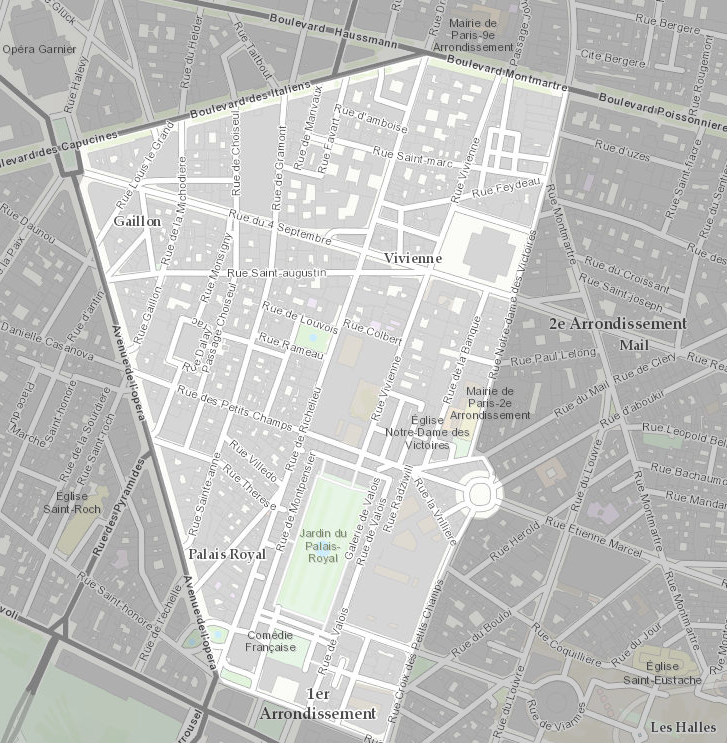
\includegraphics[width=0.5\linewidth]{images/Emprise_quartier_Richelieu.png}
    \caption{Emprise du quartier Richelieu, \mhd.}
    \label{fig:emprise_quartier}
\end{figure}

Au contraire, \enquote{Richelieu}, à comprendre comme un nom d'usage, se situe dans les quartiers Vivienne et Gaillon pour le 2\ieme~  arrondissement et dans le quartier du Palais Royal pour le 1er arrondissement. Ses axes principaux sont les rues des Petits-Champs, Richelieu, Vivienne. Il est ainsi délimité par des ensembles architecturaux tels que le Palais-Royal, l'Opéra Garnier, les grands Boulevards, la place de la Bourse et la place des Victoires (voir la figure \ref{fig:emprise_quartier})\footcite{INHACarnet2023}.

\begin{figure}
    \centering
    \includegraphics[width=0.5\linewidth]{images/BnF_quartier_Richelieu.jpeg}
    \caption{Affiche \textit{Paris, quartier Richelieu. Principales maisons de l'industrie, principales maisons du commerce} ... [placard d'annonces publicitaires pour différents commerces], 1862, Bibliothèque nationale de France, département Estampes et photographie, ENT DP-267-ROUL.}
    \label{fig:richelieu_pub}
\end{figure}


Pourquoi alors utiliser une dénomination qui \textit{a priori} n'existe pas ? En premier lieu, quelques usages ont été retrouvés dans les sources historiques: le nom est utilisé sur certaines affiches publicitaires des années 1860 (voir la figure \ref{fig:richelieu_pub}), sans doute en référence à la rue de Richelieu qui traverse le quartier. Mais quelques occurrences ne suffisent pas à donner un titre à tout un quartier. 

Surtout, ce titre renvoie aux institutions porteuses du projet Richelieu loties dans le \enquote{Quadrilatère Richelieu} ou \enquote{site Richelieu}\footcite{BNFquadrilatere2024}. Berceau historique de la \acrlong{bnf}, le site est un millefeuille architectural situé au cœur de Paris. Il est bordé à l'ouest par la rue Richelieu, au nord par la petite rue Colbert, à l'est par la rue Vivienne et au sud par la rue des Petits-Champs. Le site Richelieu a évolué au fil des siècles en passant du XVII\ieme~ siècle au XX\ieme~ siècle d'une résidence privée du cardinal Mazarin à un édifice devenu public abritant d'abord la bibliothèque royale, puis la \acrshort{bnf}\footcite{BNFLhistoire2023}. En réponse à l'évolution des besoins, la rénovation du site Richelieu, menée sur 12 ans, a entièrement réorganisé l'espace pour le consacrer à l'histoire des arts et du patrimoine. En plus des départements spécialisés de la \acrlong{bnf}, le site accueille désormais la bibliothèque de l'\acrlong{inha} et celle de l'\acrlong{enc}. Enfin, le titre du projet est le reflet d'une nouvelle clé de lecture du quartier proposée par les chercheurs, qui est au cœur de l'objet d'étude du projet de recherche. 

\section{L'objet d'étude : un enjeu historiographique}

Tout d'abord, la notion de \enquote{quartier} est historiquement remise en question. Que signifie \enquote{faire quartier}? Comme pour de nombreuses frontières nationales, les délimitations administratives des quartiers ne représentent pas les relations du voisinage, car les frontières d'un quartier \enquote{fluctuent d'un individu à l'autre}.\footnote{\enquote{Le quartier}, \textit{Le peuple de Paris au XIX\ieme~  siècle}, Miriam SIMON (dir.), Paris, Paris Musées, 2011, p.182.}\footcite{JAKOBOWICZpeuple2011} 
Quels sont alors les éléments historiques qui confèrent au quartier Richelieu son identité en tant que quartier ?  Contrairement à d'autres quartiers parisiens ou limitrophes, cet espace géographique est souvent négligé dans l'historiographie, bien qu'il se distingue par son histoire urbaine, ses activités économiques, culturelles\footcite{GRESILLONVille2008} et sociales\footcite{DIMEOgeographie2008, INHAJournee2023, INHAJournee2023a}, ainsi que par son architecture et ses usages. Sur une période de deux siècles, de 1750 à 1950, ce quartier, situé en plein cœur de Paris, a été au centre des évolutions modernes. Les institutions présentes et les aménagements urbains y ont joué un rôle majeur, notamment le \enquote{Quadrilatère Richelieu}, la Banque de France, le Palais Brongniart, le Palais Royal, le Conseil d'État, ainsi que d'autres organismes comme l'Agence France Presse. Les îlots du quartier se transforment petit à petit et non dans leur globalité, à l'instar des grands travaux de rénovation motivés par le baron Haussmann. Bien que les transformations urbaines du quartier soient ponctuelles et étalées dans le temps et l'espace\footcite{CARBONNIERderoulement2015}, il conserve une identité, une valeur culturelle et matérielle ancrée dans ses activités distinctes.

Le passage suivant, tiré d'un guide de Paris\footnote{Charles JOLIET \enquote{Les petites caves, les petites cuisines}, dans, \textit{Paris-Guide}, par les principaux écrivains et artistes de la France ; introduction par Victor Hugo, Paris, librairie internationale, 1867, p. 1558-1559. in \footcite{DUVETTEquartier2024}} de la seconde moitié du XIX\ieme~  siècle, permet d'en prendre le pouls : 

\begin{displayquote}\enquote{Cette rue est la rue Vivienne, la plus brillante et la plus animée. C'est Paris avec sa fièvre et ses mirages. Le centre topographique est la place du Châtelet, mais le vrai centre est ici. Chaque seconde, marquée par l'horloge de la Bourse, compte les pulsations du cœur de l'Europe. À cette extrémité, le Palais-Royal [...], à l'autre, le boulevard. De ce centre, en décrivant une circonférence restreinte, on englobe dix théâtres [...]. Ce monument bâti en briques et en pierres de taille déployant sa double façade, c'est la Bibliothèque qui renferme dans ses catalogues l'héritage de toutes les littératures [...]. Chaque boutique qui sollicite ton regard est une exposition spéciale et choisie. Voici une machine à vapeur, des objets d'art, l'antiquité et la mode ; là une boutique de libraire, le musée de la gastronomie, un magasin de fleurs, des tableaux, des gravures, des bronzes, les photographies des célébrités des lettres, des sciences, des arts, de la chaire, du barreau, de la politique, de la cour, de la ville et du théâtre ; dans ce kiosque, cent journaux ; devant toi la poste et le télégraphe : ici, des hôtels, des cercles, des cafés, des passages. En deux heures avec l'or que nous n'avons pas, on peut y organiser sa vie}.
\end{displayquote}

Bien que cet extrait romancé ne capture qu'un instantané de la rue Vivienne, il décrit une artère centrale, un passage clé du quartier, au cœur d'un réseau plus vaste. La rue Vivienne relie le Palais Royal et les théâtres, mène au Palais Brongniart, à la place des Victoires ou encore à l'Opéra Garnier et invite à flâner\footcite{WALTERParis1989} parmi les boutiques des galeries Vivienne et Colbert. L'ambiance qui s'en dégage à travers les siècles contribue au symbolisme du quartier, où cohabitent des images mythiques et parfois contradictoires, façonnant ainsi une représentation mentale de Paris au XIX\ieme~  siècle\footcite{CHOAYPour2009} jusqu'à nos jours\footcite{SAWYERCartographie2011}. En ce sens, l'étude du quartier Richelieu devient un exemple de la manière dont habitants et passants perçoivent et construisent leur espace\footcite{LEFEBVREproduction1974}. Ces représentations constituent une clé essentielle pour analyser la dynamique des quartiers parisiens\footcite{DUVETTECulture2024}. C'est à partir d'une approche interdisciplinaire, mêlant histoire, géographie, urbanisme, architecture, histoire de l'art, topographie, économie et sociologie, qu'émerge la définition du \enquote{quartier Richelieu}.

Plus largement, ce projet vise à comprendre l'émergence de l'archétype de la capitale moderne, tel qu'il s'est imposé depuis le début du XIX\ieme~  siècle en Europe\footcite{CHARLEStemps2009, CHARLECapitales2023}, en prenant le cœur névralgique de Paris comme point de référence.

\section{Les acteurs et collaborateurs : un engouement institutionnel}
\enquote{C'est sous l'impulsion de plusieurs institutions publiques, regroupées dans un périmètre géographique}\footcite{DUVETTEquartier2024} présenté précédemment que né le projet \enquote{Richelieu. Histoire du quartier}. 

\subsection{Les partenaires institutionnels...}
Conjointement la \acrshort{bnf}, l' \acrshort{inha}, l'\acrshort{enc}, le Centre André Chastel de Sorbonne Université, le \acrlong{dfk} (DFK)\footnote{Depuis 2021 l'\acrlong{epfl} (EPFL) a également rejoint le rang des partenaires.} proposent de se réunir autour d'un projet collectif dédié à \enquote{ une investigation collective de l'histoire du quartier dans lequel elles sont implantées}\footcite{PROJETFondation2021}. L'intérêt de mettre en synergie ces institutions réside d'une part dans la richesse de leurs ressources documentaires et d'autre part dans leur expertise en matière d'histoire de l'art et du numérique. Le consortium culturel ainsi créé, le projet obtient le soutien financier de la \acrlong{fsp}(FSP), à deux reprises en \href{https://www.sciences-patrimoine.org/projet/rich-data/}{2021 sous le titre \enquote{RICH.DATA}} et en \href{https://www.sciences-patrimoine.org/projet/richdata2/}{2023 pour \enquote{RICH.DATA II}}\footnote{Cliquer sur le nom des projets pour accéder aux pages web correspondantes.}, et de la \acrlong{bdf} (BdF) permettant la constitution d'une équipe de recherche et d'ingénierie. 

\subsection{... et les équipes de recherche et d'ingénierie ...}
La dimension numérique du projet de recherche en histoire de l'art et de l'architecture implique des acteurs d'horizons divers. 

 
\subsubsection{Les chercheurs} 

Tout d'abord, des chercheurs, en l'occurrence deux chercheuses: Isabella di Lenardo, historienne de l'art de formation et spécialiste des humanités numériques pour les reconstitutions urbaines italiennes\footnote{Isabella di Lenardo est aujourd'hui coordinatrice du projet Time Machine Unit au Collège des humanités numériques de l'\acrshort{epfl}, dont le site est accessible \href{https://www.epfl.ch/schools/cdh/time-machine-unit/team/}{ici}.}, a mené la première phase du projet de 2018 à 2020. Elle a également lancé le premier volet numérique intitulé RICH.DATA du projet Richelieu. Puis, Charlotte Duvette, historienne de la ville et de l'architecture, s'intéressant aux transformations, représentations et publications sur Paris entre le XVIII\ieme~ et le XIX\ieme~  siècle\footnote{Charlotte Duvette est aujourd'hui Maîtresse de conférences associée à l'École d'architecture de Rennes, depuis où elle assure également la finalisation du projet.}, lui succède de 2021 à 2024 - pour la seconde et peut-être dernière phase du projet. Chacune, considérée comme cheffe du projet Richelieu, a respectivement contribué à chaque phase du projet. Isabella di Lenardo, principalement affiliée au Département de la bibliothèque de l' \acrshort{inha}, a constitué le premier corpus textuel. En tant que membre du \acrlong{der} (DER) de l' \acrshort{inha}, Charlotte Duvette a construit les corpus iconographique et cartographique. Les corpus seront présentés en détail par la suite. Chacune des chercheuses est accompagnée de doctorantes chargées d'études et de recherche (\acrshort{cer}) de l' \acrshort{inha} et de stagiaires masterants. Ensemble, ils s'occupent de définir les axes de recherche pour constituer les corpus, de publier et communiquer sur les questions de recherche du projet. Par exemple, Justine Gain (\acrshort{cer}) a participé à la formation d'un nouveau corpus autour du Palais-Royal de 2022 à 2023. Entre 2023 et 2024, Louise Thiroux (\acrshort{cer}) a complété ce corpus en associant chaque iconographie à un lieu, en définissant et en classant les thèmes et entités nommées, ainsi qu'en rédigeant plusieurs articles scientifiques. Pour les stagiaires les plus récents, Teoman Akgönül (\acrshort{cer}) s'est vu confier la mission de collecter, classifier et annoter les images documentant l'activité liée aux rue adjacentes de la Banque de France. Son corpus de recherche est principalement constitué des éphémères produits par les restaurants du quartier. Tous, ils ont construit l'objet d'étude du projet Richelieu qui est alors structuré par les ingénieurs.

 
\subsubsection{Les ingénieurs}
 
Les ingénieurs constituent la deuxième face indissociable du projet. Comme pour les cheffes du projet Richelieu, deux ingénieurs se sont succédés. Loïc Jeanson, ingénieur de formation, est arrivé en 2021 en tant que post-doctorant pour le premier volet numérique, RICH.DATA. Il a principalement participé à la création du \acrlong{sig}  (SIG) du quartier Richelieu. Puis, Paul Kervegan lui a succédé dès 2022, et ce jusqu'à la fin de la phase actuelle du projet, \enquote{RICH.DATA II}\footcite{PROJETFondation2023}. Formé à l'École du Louvre et diplômé du Master \acrshort{tnah} de la promotion 2022, il est à même de connaître les enjeux des technologies numériques appliquées à l'histoire de l'art. Il a encodé, modélisé et traité les données du projet dont il a aussi développé l'exposition sur la plateforme Richelieu. En tant qu'ingénieur principal du projet, il a aussi été accompagné de stagiaires : Collin Prudhomme, issu du Master Humanités numériques de l'\acrshort{enc} en 2023, qui s'est chargé du développement du modèle \acrshort{3d} affilié au corpus iconographique et, moi-même qui a participé au développement de l'outil cartographique. 

\subsection{...forment le comité de pilotage du projet.}
S'ajoute un comité de pilotage qui assure la coordination de l'ensemble des travaux de recherche et d'ingénierie. Il est principalement composé de représentants des institutions partenaires\footnote{Celui-ci est notamment composé de France Nerlich et Juliette Trey ( \acrshort{inha}), Frédéric Kaplan (Directeur du Collège des humanités à l'\acrshort{epfl}), Isabella di Leonardo (\acrshort{epfl}), Gennaro Toscano (Conseiller pour la recherche et la valorisation et coordinateur scientfique des collections du musée), Olivier Jacquot (Responsable de la coordination de la recherche à la \acrshort{bnf}), Philippe Chevallier (Adjoint au responsable de la coordination de la recherche, \acrshort{bnf}), Elsa Marguin-Hamon (Directrice de la recherche à l'ENC), Peter Geimer (Directeur du \acrshort{dfk}), Jean-Baptiste Minnaert (Professeur d'histoire de l'architecture, Centre André Chastel).} et des équipes de chercheurs et d'ingénieurs. Jusqu'au départ de la Directrice du \acrshort{der} à l' \acrshort{inha}, France Nerlich était à la tête du comité puis, Juliette Trey, Directrice par interim, s'est occupée du suivi administratif, financier et scientifique. Les responsables scientifiques, de collections ou de recherche se réunissent tous les 3 mois environ. Les avancées du projet leur sont présentées et des décisions sont prises quant aux calendriers de rendus, aux communications scientifiques (articles, conférences, journée d'études), au design graphique et interactif du projet final. À intervalle plus régulier, et voyant la date butoire du projet approcher, se réunissent également les membres de l'\acrshort{inha} du projet, soit Juliette Trey, Federico Nurra, Charlotte Duvette, Paul Kervegan et les stagiaires pour la partie recherche, ingénierie et design graphique le cas échéant. 

\subsection{D'autres collaborations}
Dans ce large périmètre institutionnel, le projet mène également d'autres collaborations. L'équipe du projet a recours au réseau professionnel interne à l'\acrshort{inha}. Par exemple, la veille technologique du projet est assurée par le chef du \acrshort{snr}, Federico Nurra, archéologue de formation, dont son expertise sur les systèmes d'informations géographiques et la cartographie Web est mise à profit. En outre, il s'occupe aussi de fédérer les équipes numériques des différents établissements pour RICH.DATA II. Tandis que Jean-Christophe Carius, ingénieur du projet \acrlong{pense}\footnote{\href{https://pense.inha.fr/}{\acrshort{pense}} est la Plateforme d'Éditions Numériques de Sources Enrichies de l' \acrshort{inha} (Cliquer sur le nom du projet pour accéder au site Web). Elle est développée comme un atelier de fabrication numérique autour de la question de la publication en ligne de sources en histoire de l'art de toute nature (images, manuscrits, correspondances, archives…). Il s'est notamment concentré sur le projet des Papier Antoine-Louis Barye, Les décors Karbowsky.}, et Chloé Pochon, ingénieure chargée de la curation des données, apportent leur expertise en développement informatique et en création de la plateforme cartographique.
L'équipe collabore également avec le laboratoire InVisu\footnote{InVisu est un laboratoire de recherche en Histoire de l'art qui met à profit es outils du numérique pour accompagner les renouveaux méthodologiques en histoire de l'art comme dans les sciences sociales en général, prêtant une attention particulière à la matérialité et à l'inscription dans la société des objets visuels, décoratifs, usuels et architecturaux. Le site Web est disponible \href{https://invisu.cnrs.fr/}{ici}.} affilié à l' \acrshort{inha} dont Manuel Charpy en est le directeur. Le projet a ainsi bénéficié des compétences en design graphique de Lou Ong, stagiaire graphiste, qui a proposé plusieurs pistes de design pour la page initiale et la navigation entre les pages et corpus du site web. 

L'\acrshort{inha} a développé des collaborations externes dont profite le projet Richelieu de par son intégration au SNR. Par exemple, le Consortium Huma-Num\footnote{Les Consortiums de Huma-Num\href{https://www.huma-num.fr/les-consortiums-hn/}{, dont le site est disponible ici}, l'infrastructure de recherche dédiée aux lettres, sciences humaines et sociales dont l'histoire et l'histoire de l'art et les humanités numériques, permet de réunir des personnels scientifiques d'unités et équipes de recherches aux métiers variés (chercheur, ingénieur, archiviste, documentaliste) autour de thématiques et d'objets communs.} Projets Time Machine qui réunit plus de 27 partenaires nationaux et internationaux\footcite{CSTPTMDemande2022}. Grâce à ce partenariat, les données et les résultats peuvent être diffusés auprès d'une large communauté scientifique. De plus, le projet Richelieu participe à l'élaboration des procédures et standards numériques partagés autour d'une thématique commune, en l'occurrence les données géohistoriques spatialisées du projet Richelieu et la valorisation spatiale des collections iconographiques en histoire de l'art - nous y reviendrons plus en détail.

Pour finir, le projet a collaboré avec l'UMR 395 \acrshort{cnrsmc} MAP\footnote{L'\href{https://www.map.cnrs.fr/fr/le-laboratoire/historique/ancienne-umr-3495/}{Site de l'UMR MAP}}, sous la direction de Livio de Luca, jusqu'à ce que celle-ci ferme pour devenir laboratoire MAP UPR\footnote{\href{https://www.map.cnrs.fr/}{Site du MAP UPR}}.

Ainsi, le projet Richelieu évolue dans un écosystème riche, profitant des collaborations internes et externes à l' \acrshort{inha}, tant au niveau national qu'international. 

\section{Les corpus documentaires : des sources historiques}
L'approche documentaire se veut exhaustive pour remonter dans le temps et explorer le quartier de 1750 à 1950. Cela implique de rassembler un volume substantiel de données historiques. Quelles sont donc les sources qui témoignent de l'histoire du quartier ? Où et comment ces sources ont-elles été collectées ? Quelles méthodes ont été employées et pour quelles raisons ? À quelle typologie ces sources appartiennent-elles et quelle est leur nature ? Jusqu'à quel degré de précision vont-elles ? Se limitent-elles à une vue d'ensemble de la ville ou s'intéressent-elles à des détails aussi spécifiques qu'un bouton de porte ? Ces questions sont au cœur de cette section, consacrée aux corpus documentaires réunis pour reconstituer le quartier Richelieu.

Il convient d'informer le lecteur que les corpus textuel, cartographique et iconographique étaient initialement considérés comme d'importance égale et constituaient les principaux ensembles de données du projet Richelieu. Après analyse des résultats de l'exploration documentaire, il a été décidé que le corpus textuel est secondaire car les données ne sont pas assez exploitables. Puis, le relevé lasergrammetique, occupe également une place secondaire car il se concentre sur un petit fragment du quartier. C'est pourquoi les corpus secondaires seront succintement abordés. 


\subsection{Les principaux corpus : les sources primaires}
Au départ, les partenaires du projet avaient pour ambition de se concentrer sur leurs propres collections patrimoniales pour reconstituer l'histoire du quartier. Par exemple, la \acrshort{bnf} conserve des fonds d'architectes tels que ceux de Louis Visconti ou Henri Labrouste, ainsi que des recueils, revues d'architecture, affiches et séries topographiques du quartier, également conservées à l' \acrshort{inha}. Cependant, ces institutions ne détiennent pas l'exclusivité de ces sources. De nombreuses autres collections patrimoniales, qu'elles soient parisiennes, privées ou étrangères, disposent également de documents historiques sur le quartier Richelieu. Reconstituer l'histoire d'un quartier exige en effet de croiser et de confronter diverses sources. Les chercheurs impliqués dans le projet ont ainsi mené des recherches spécifiques, mettant en lumière des documents jusque-là inaccessibles (parfois non inventoriés) ou inexplorés. Un état des lieux des sources disponibles a été en partie dressé lors de cycles de séminaires à l' \acrshort{inha}. Le premier, intitulé \enquote{Richelieu. Histoire du quartier : état des lieux }, s'est tenu de 2018 à 2019 et a présenté les sources issues des institutions; le deuxième cycle intitulé \enquote{Documenter l'histoire urbaine, architecturale, sociale et culturelle du quartier Richelieu (1750-1950)} a réorienté les recherches sur le corpus iconographique de 2021 à 2022; le troisième cycle  de séminaires de 2022 à 2024 a quant à lui ouvert les échanges aux enjeux du numérique en sciences humaines et sociales : \enquote{Étudier la ville : un dialogue entre pratiques numériques et histoire de l'art}. A l'issue de ces échanges et recherches, une contrainte a orienté la sélection des sources : seuls les documents déjà numérisés ont été retenus pour constituer le corpus du projet. 

\subsubsection{Le corpus cartographique}
Dès le début du projet, les cartes anciennes, les plans cadastraux et les atlas ont été recensés comme des sources essentielles pour visualiser l'évolution du quartier au fil du temps. Ces documents permettent de comparer, par exemple, les changements parcellaire et viaire. Les fonds sélectionnés proviennent du Département des cartes et plans de la \acrshort{bnf}, des Archives nationales, des Archives de Paris, ainsi que des collections de Paris Musées. Parmi les sources spécifiques, on trouve l'Atlas Vasserot, un cadastre par îlots réalisé par Philibert Vasserot entre 1810 et 1836, conservé aux Archives nationales\footnote{Des versions numérisées sont consultables sur le site ici, de CP/F/31/73 à 96} ; le plan parcellaire municipal de Paris de 1900, conservé aux Archives de Paris \footnote{Des versions numérisées sont consultables sur le site \href{https://archives.paris.fr/f/planspacellaires/tableau/?&crit1=14&v_14_1=02}{ici}, de PP/11870/A à F, de PP/11880/A à C, de PP11914/A à C}; les plans cadastraux dits napoléoniens, comprenant 26 000 feuilles couvrant les 12 arrondissements de Paris de 1809 à 1854\footnote{Des versions numérisées sont consultables sur le site \href{https://www.siv.archives-nationales.culture.gouv.fr/siv/rechercheconsultation/consultation/ir/consultationIR.action?irId=FRAN_IR_059652}{ici}, de CP/F/31/3 à 14} conservés aux Archives nationales (voire le plan \ref{fig:plan_carto_RR65} ci-contre); et le plan Billaud  qui préfigure les galeries Vivienne et Colbert autour de 1827, conservés au Musée Carnavalet (voir le plan \ref{fig:plan_carto_galeries} ci-contre). Enfin, il y a aussi des plans dits contemporains, en cours de sélection. Parmi ces ensembles, seules les sections de plans ou feuilles couvrant la zone du quartier Richelieu, telle que définie par le projet, sont sélectionnées et intégrées au corpus cartographique. Au total, presque 500 découpes de plans sont sélectionnées, dont une majeure partie ont pour source le parcellaire de 1900 en raison de leur échelle très réduite (voir le tableau \ref{tab:total_carto}). 

\begin{figure}[!]
    \centering
    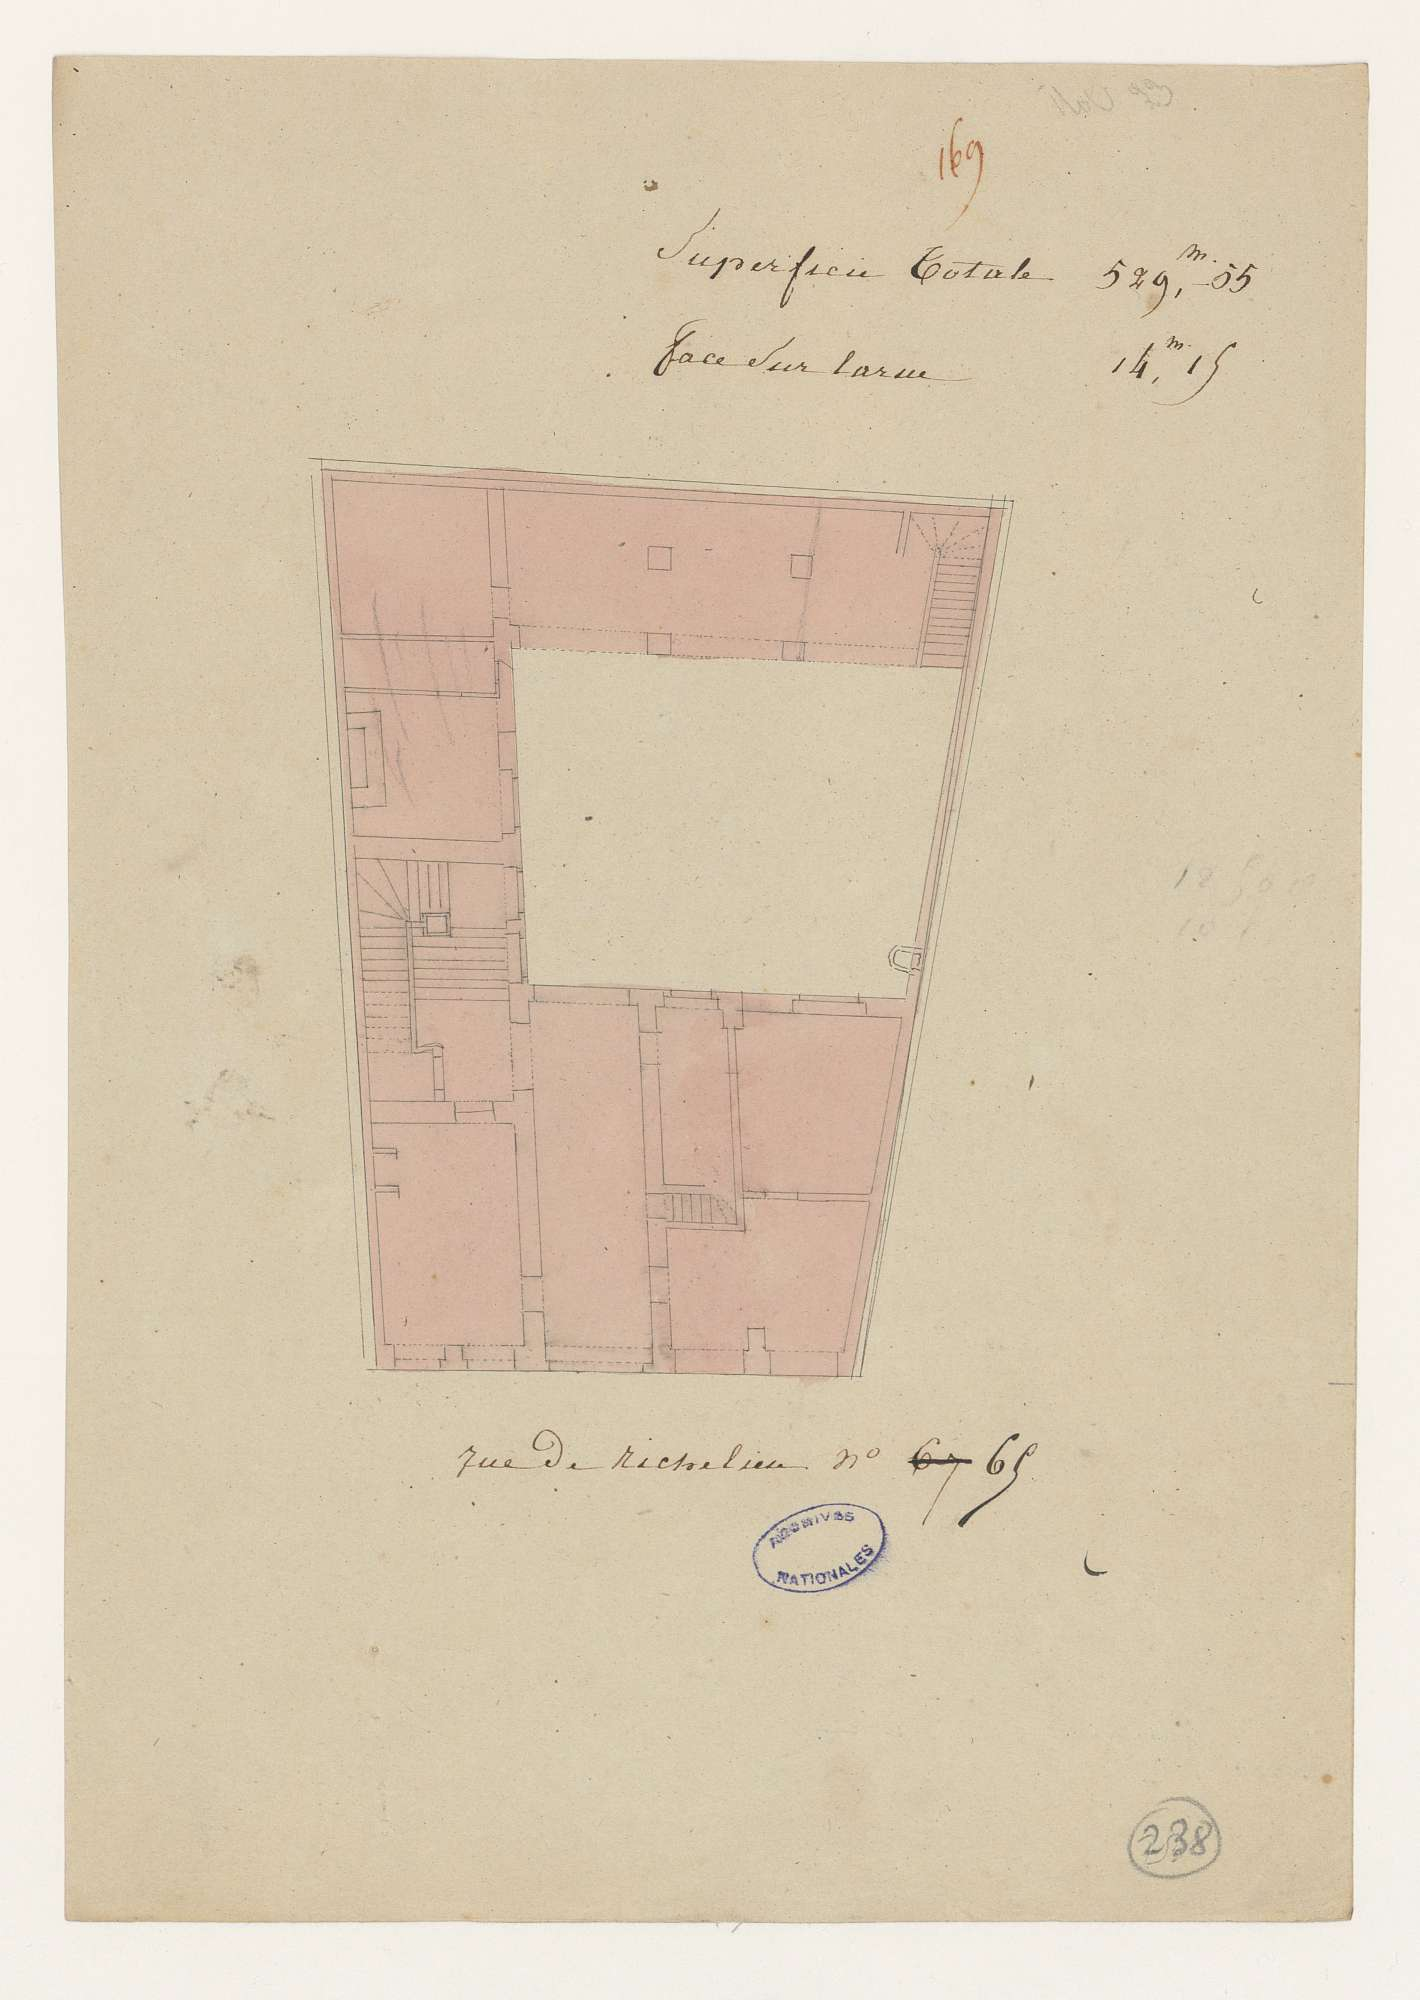
\includegraphics[width=0.5\linewidth]{images/AN_65_Richelieu.jpg}
    \caption{Plans cadastraux dit à la feuille de Paris 1809-1854, 65 rue de Richelieu, AN, \href{https://www.siv.archives-nationales.culture.gouv.fr/siv/media/FRAN_IR_058572/d_2851/FRAN_0198_3023_L}{CP/F/31/9 n°238}.}
    \label{fig:plan_carto_RR65}
\end{figure}

\begin{figure}[!]
    \centering
    \includegraphics[width=0.5\linewidth]{images/ParisMusees_Billaud.jpg}
    \caption{Plan de la Galerie et de la Rotonde Colbert, Billaud, Musée Carnavalet.}
    %\href{{https://www.parismuseescollections.paris.fr/fr/musee-carnavalet/oeuvres/plan-des-galeries-et-rotonde-colbert-conduisant-de-la-rue-vivienne-a-la-0#infos-principales}{num inv}.}
    \label{fig:plan_carto_galeries}
\end{figure}


\begin{table}[!]
\centering
\label{tab:total_carto}
    \begin{tabular}{|l|c|}
    \toprule
    \textbf{Source cartographique} & \textbf{Nombre} \\ 
    \midrule
    Contemporain & 26 \\
    Billaud & 22 \\
    Feuille & 97 \\ 
    Vasserot & 116 \\
    Parcellaire 1900 & 234 \\
    \midrule
    \textbf{Total} & \textbf{495} \\
    \bottomrule
\end{tabular} 
\caption{Calcul du nombre de documents par source cartographique.}
\end{table}

Des fonds de cartes\footcite{ESRIDefinition2024} de Paris de différentes époques viennent compléter le corpus : le plan Verniquet de 1791\footnote{Une version numérisée du plan Verniquet est disponible sur Gallica, le site \href{https://gallica.bnf.fr/view3if/ga/ark:/12148/btv1b55013275x}{ici}.}, le plan Dubrueil de 1856\footnote{Une version numérisée du plan Dubreuil est consultable sur Gallica, le lien \href{https://gallica.bnf.fr/view3if/ga/ark:/12148/btv1b53085562p}{ici}.}, et un plan municipal de 1910-1920 en cours de sélection. Ils sont tous numérisés et disponibles soit à la \acrshort{bnf} soit dans les bibliothèques spécialisées de Paris pour le plan Andriveau-Goujon de 1867\footcite{ANDRIVEAU-GOUJONPlan1867}.

Ces documents sont les sources primaires largement référencées et numérisées. Nous verrons par la suite quelle est la distinction que le traitement informatique effectue sur les sources cartographiques entre les plans et les fonds de carte, en raison des référentiels géohistoriques.
 
\subsubsection{Le corpus iconographique}

Le corpus iconographique s'est constitué au cours de la seconde phase du projet. L'équipe de chercheurs a effectué un repérage systématique des corpus iconographiques numérisés et conservés dans diverses institutions parisiennes et internationales. Ces documents, très variés, proviennent principalement de la \acrshort{bnf}, de l' \acrshort{inha}, de Paris Musées (dont le Petit Palais, le Musée Carnavalet, le Musée de la Vie Romantique, le Palais Galliera, la maison de Balzac, la maison de Victor Hugo, le Musée Bourdelle et le musée de la Libération Leclerc Moulin), ainsi que des Archives nationales, des Archives de la Ville de Paris, des bibliothèques spécialisées de Paris, et du British Museum. Les représentations graphiques, telles que les photographies, cartes postales, estampes, gravures (voir la figure \ref{fig:palais_royal1789}), dessins, croquis d'architectes et même peintures (voir la figure \ref{fig:clair_lune}), offrent un aperçu visuel de différentes époques, capturant l'architecture, l'aménagement des rues (voir la photographie \ref{fig:urinoir}), les événements, les passants, et parfois des scènes de la vie quotidienne. En plus de cela, des documents comme des coupures de presse, des affiches publicitaires, ainsi que des éléments plus inattendus tels que des jetons de commerce, des menus de restaurant, et des cartes de visite ont été sélectionnés. Au total, plus d'une centaine de typologies différentes forment un corpus iconographique hétérogène, rassemblant un total de plus de 5000 documents (voir le tableau \ref{tab:iconographie_institution}).

\begin{figure}[ht!]
    \centering
    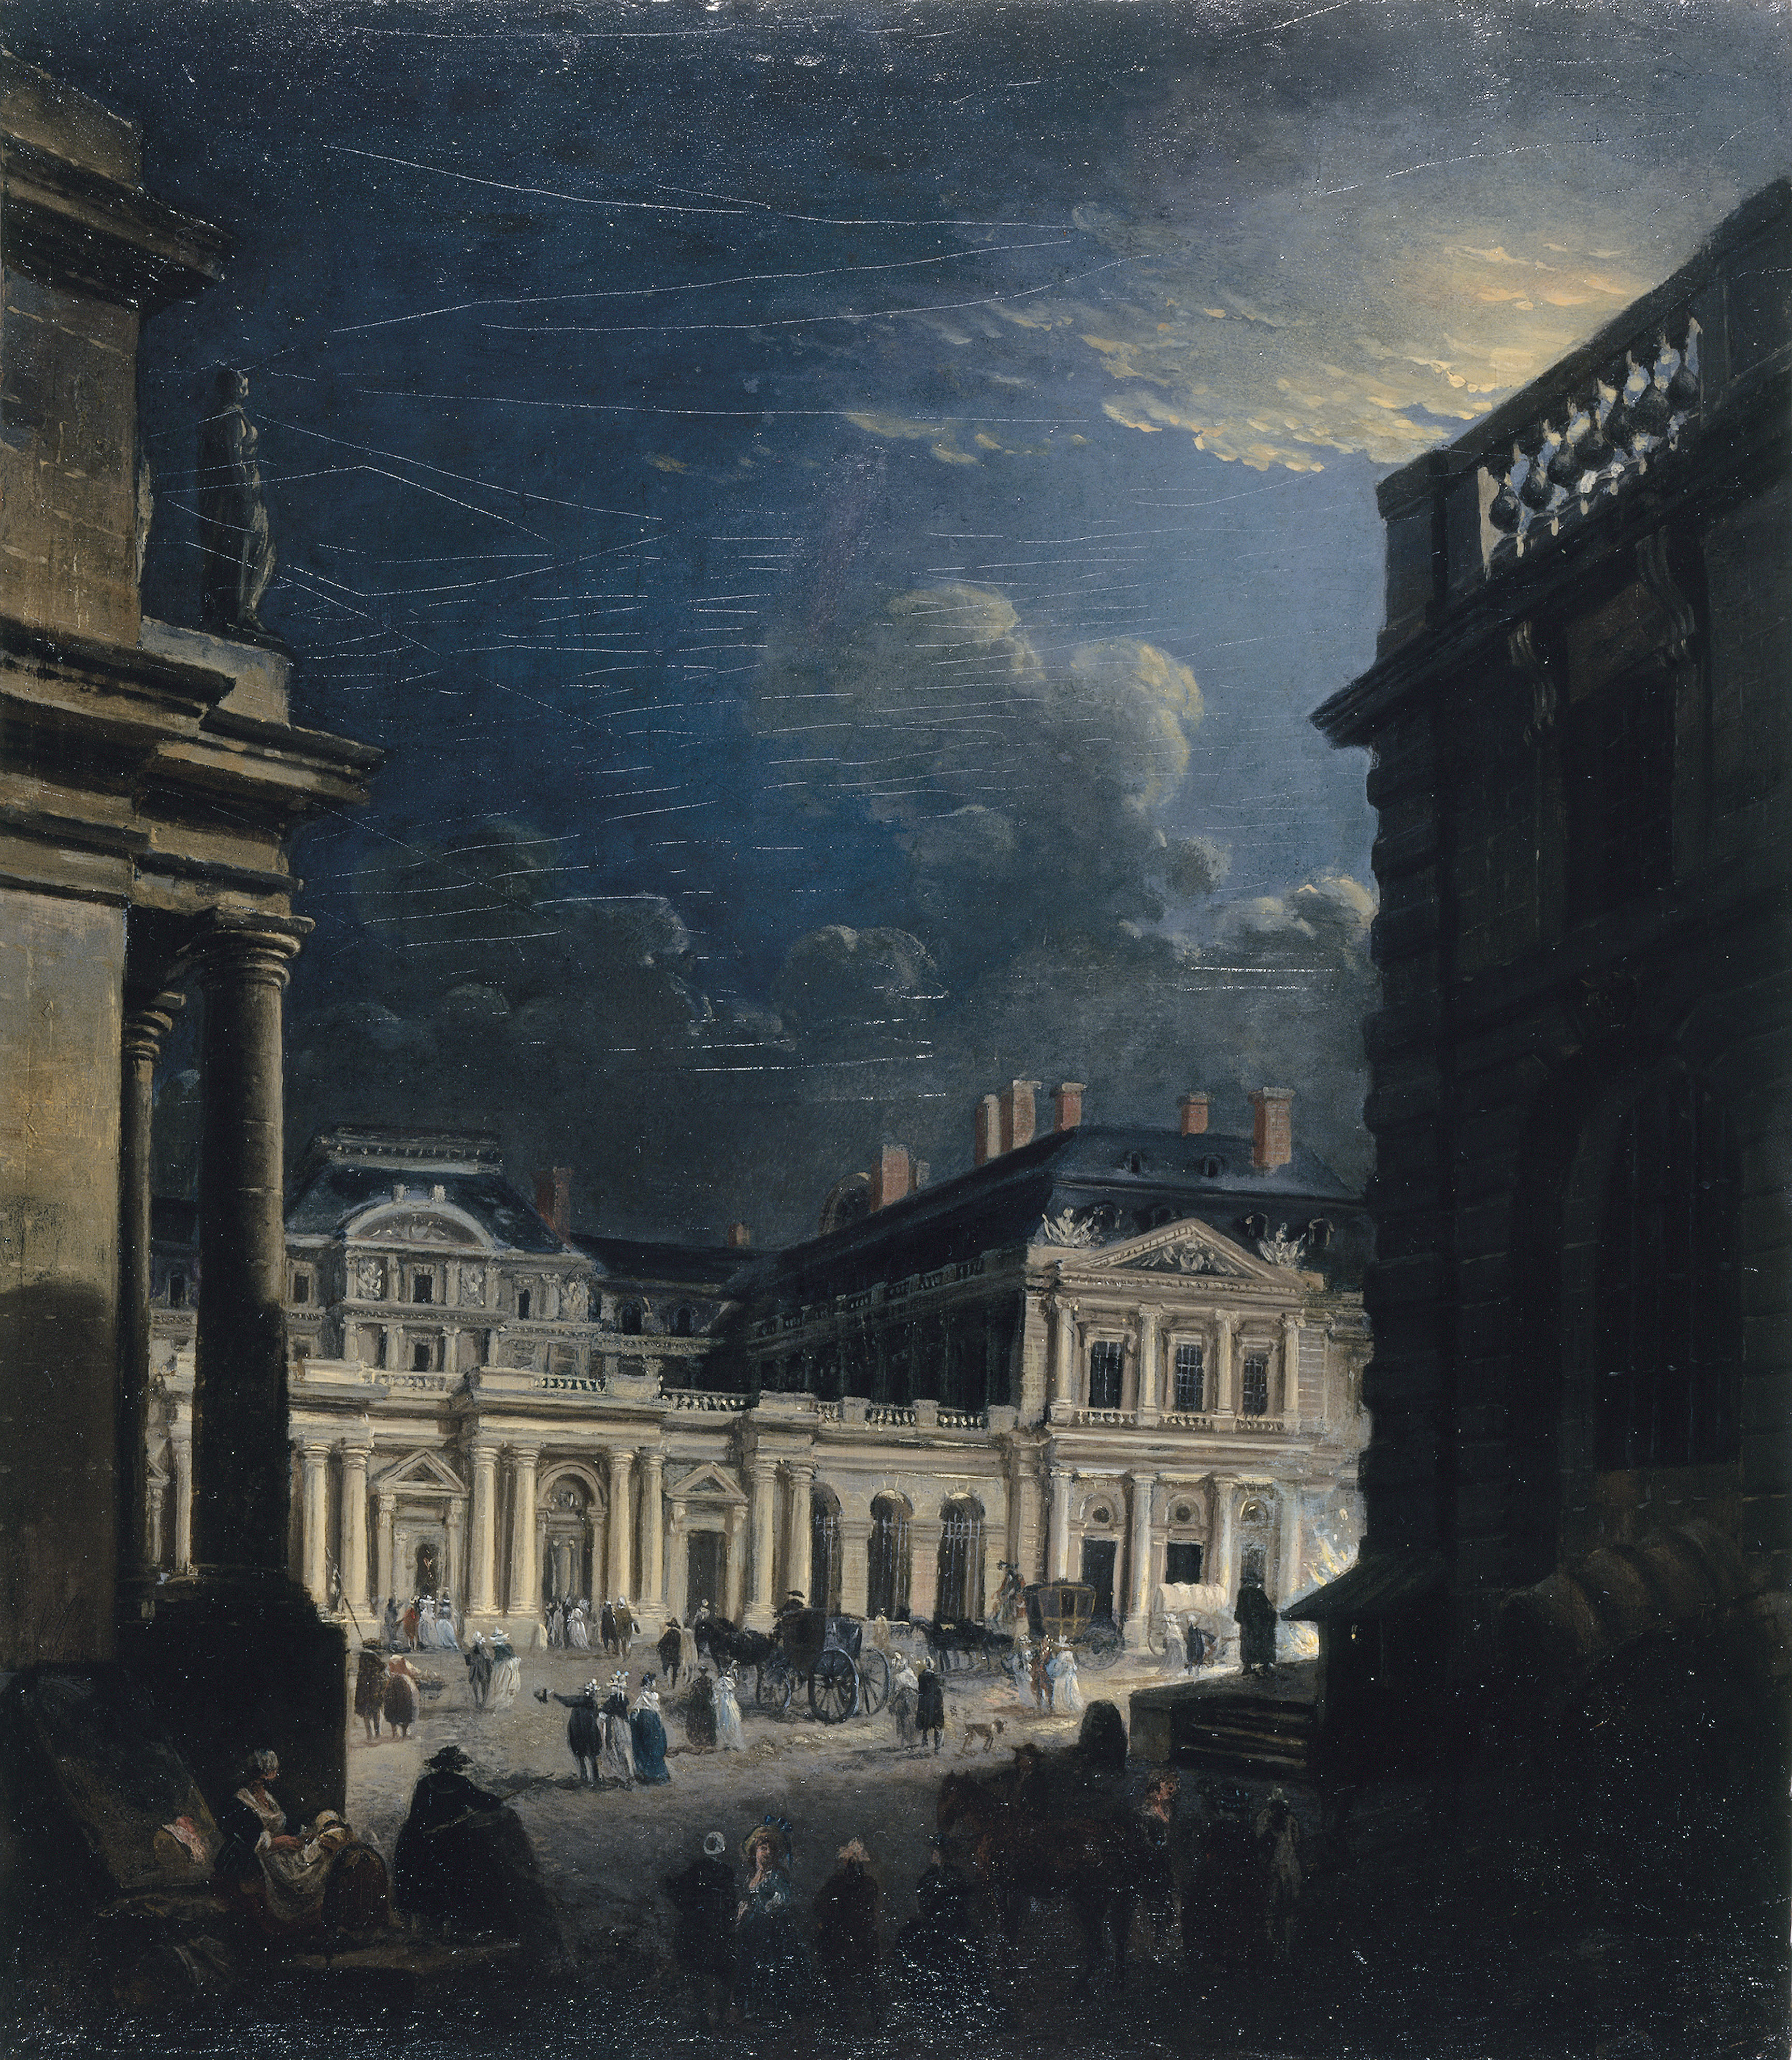
\includegraphics[width=0.5\linewidth]{images/palais_royal_clairdelune.jpg}
    \caption{Pierre-Antoine Demachy (1723 - 1807), \textit{La Place du Palais Royal, au clair de lune}, vers 1765, Huile sur toile, 39,5 x 34 cm, Musée Carnavalet, P93.}
    \label{fig:clair_lune}

%https://www.parismuseescollections.paris.fr/fr/musee-carnavalet/oeuvres/la-place-du-palais-royal-au-clair-de-lune#infos-secondaires-detail 
\end{figure}
\begin{figure}[ht!]
    \centering
    \includegraphics[width=0.7\linewidth]{images/vue_palais_royal1789.jpg}
    \caption{Première vue du jardin du Palais Royal, prise de la Rotonde, Paris, Aubert, 1789, Musée Carnavalet,  }
    \label{fig:palais_royal1789}
\end{figure}

\begin{figure}[ht!]
    \centering
    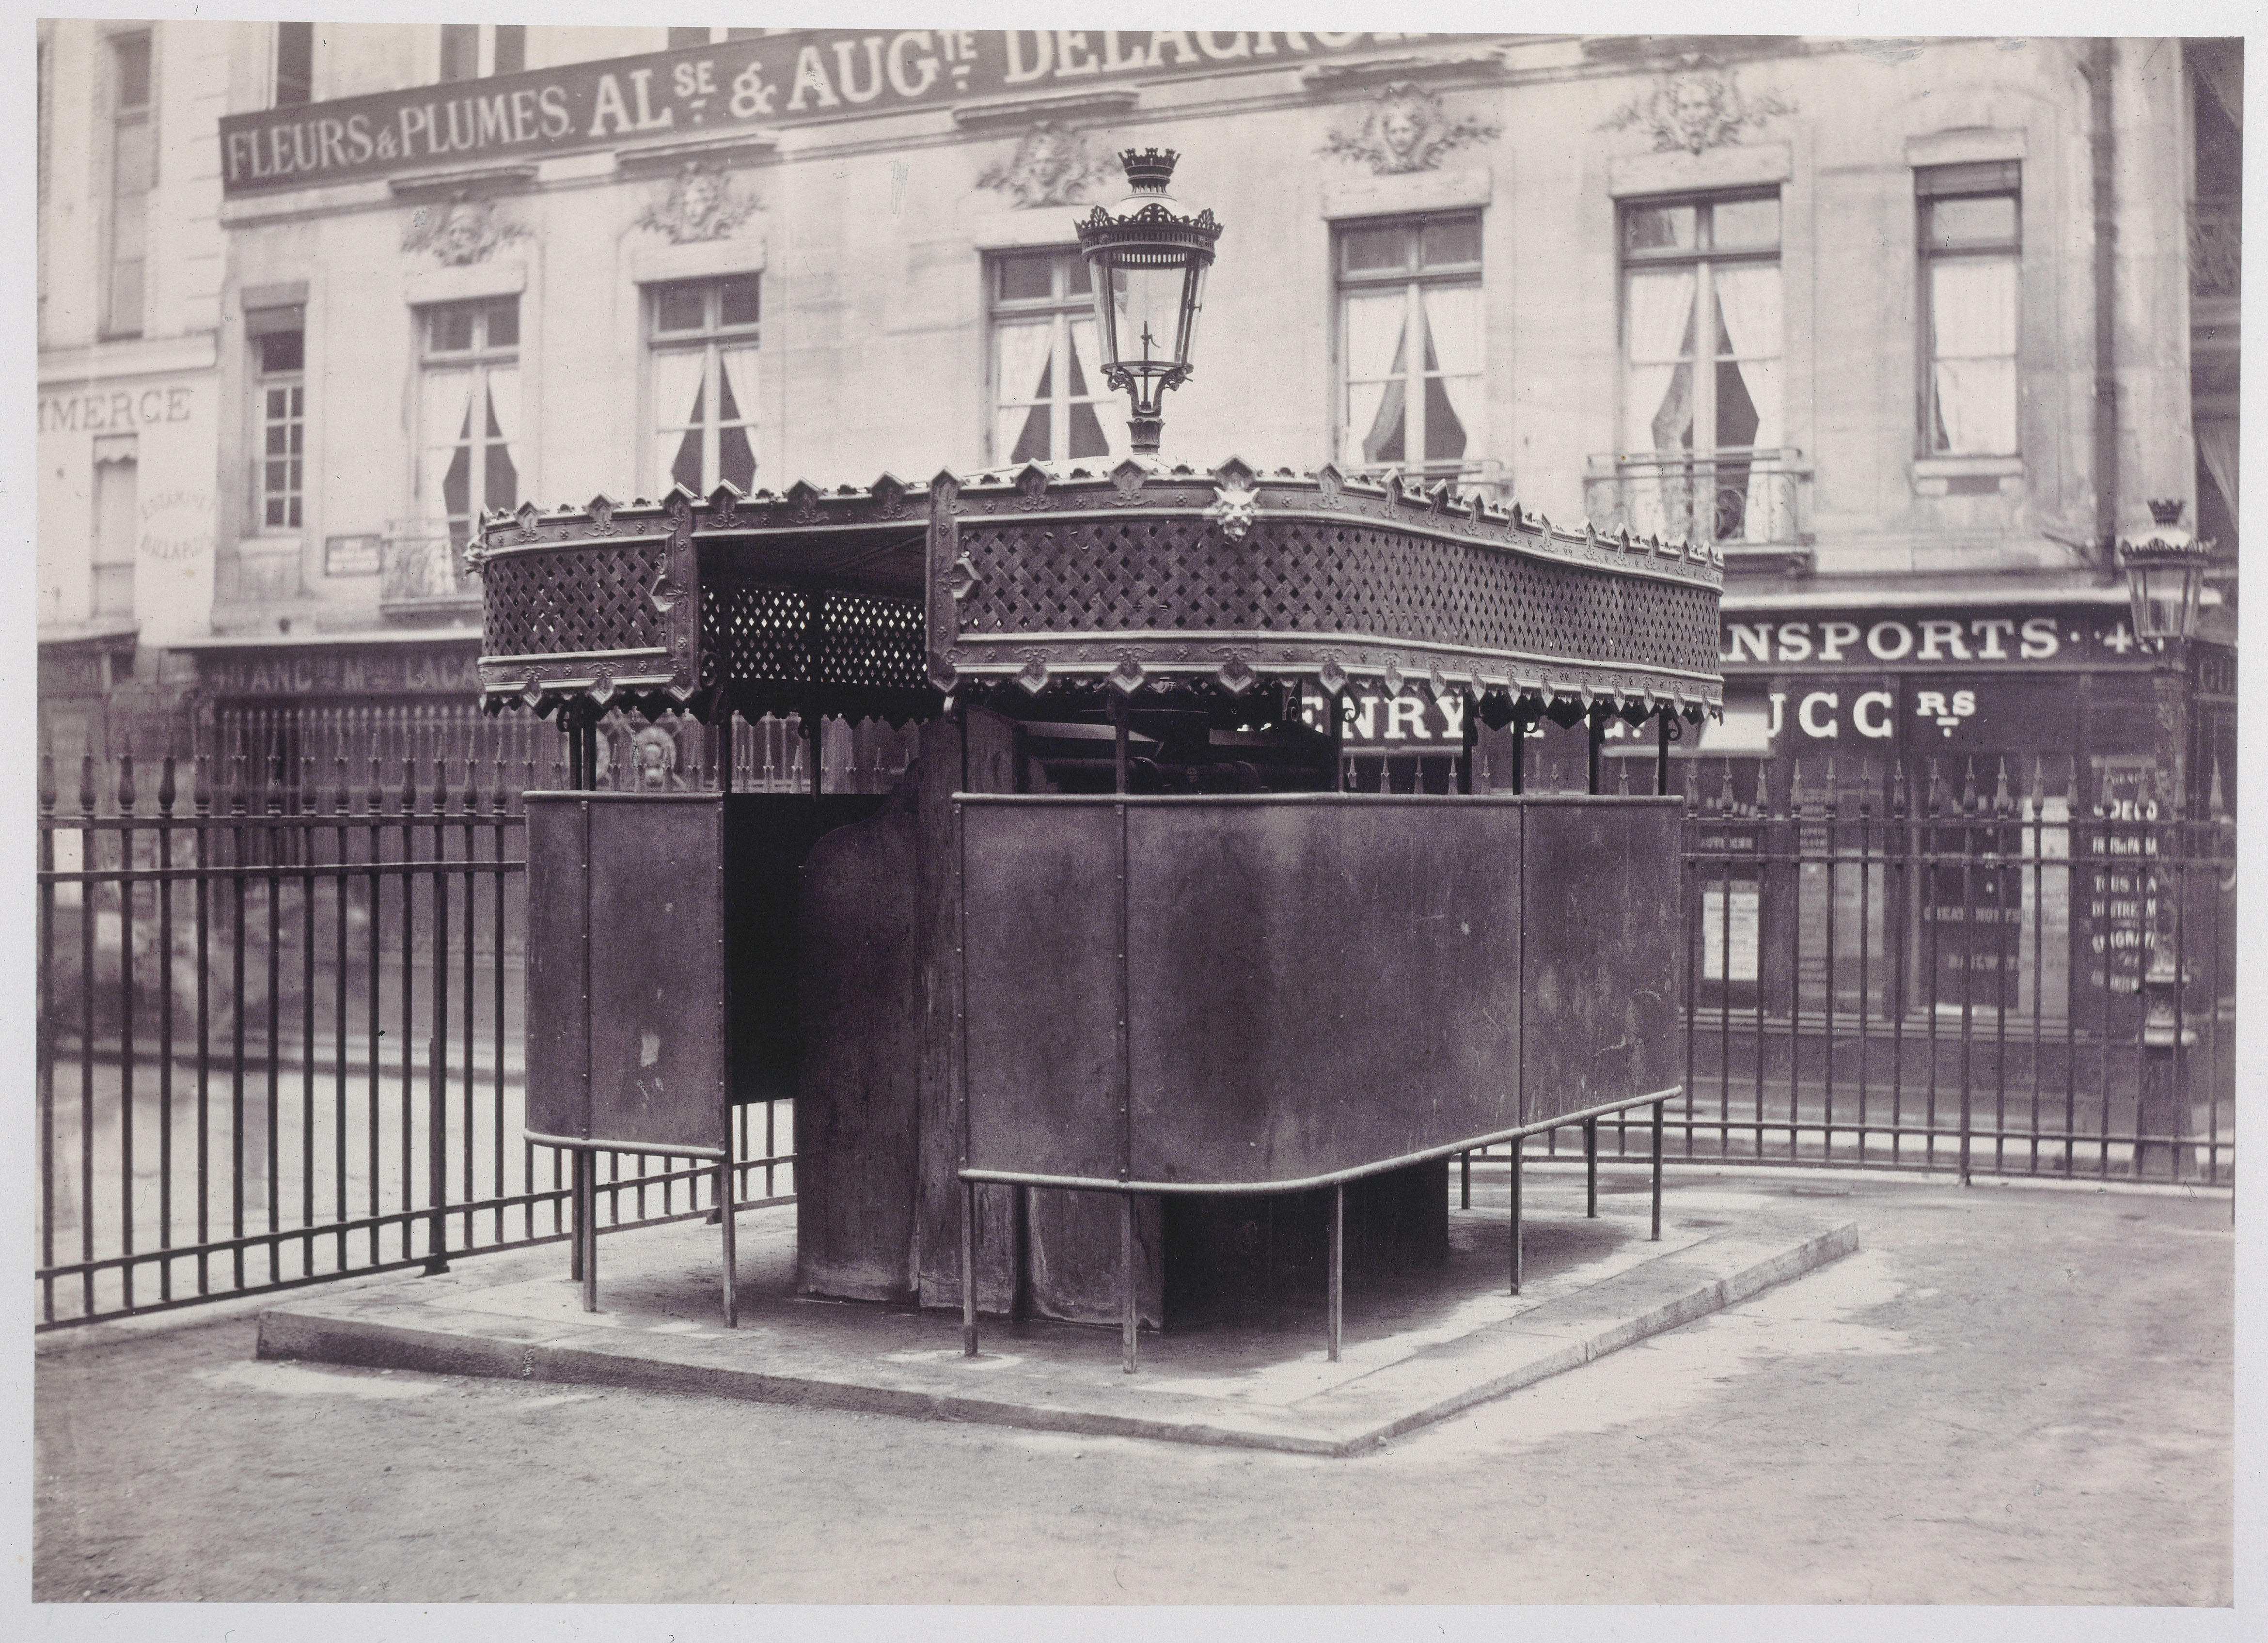
\includegraphics[width=0.7\linewidth]{images/urinoir_marville.jpg}
    \caption{Urinoir enveloppé à six stalles, jardin de la Bourse, place de la Bourse, Paris, Marville, photographie, seconde moitié du XIX\ieme~ siècle, Musée Carnavalet, PH4147.}
    \label{fig:urinoir}
\end{figure}

% \begin{figure}[ht!]
%     \centering
%     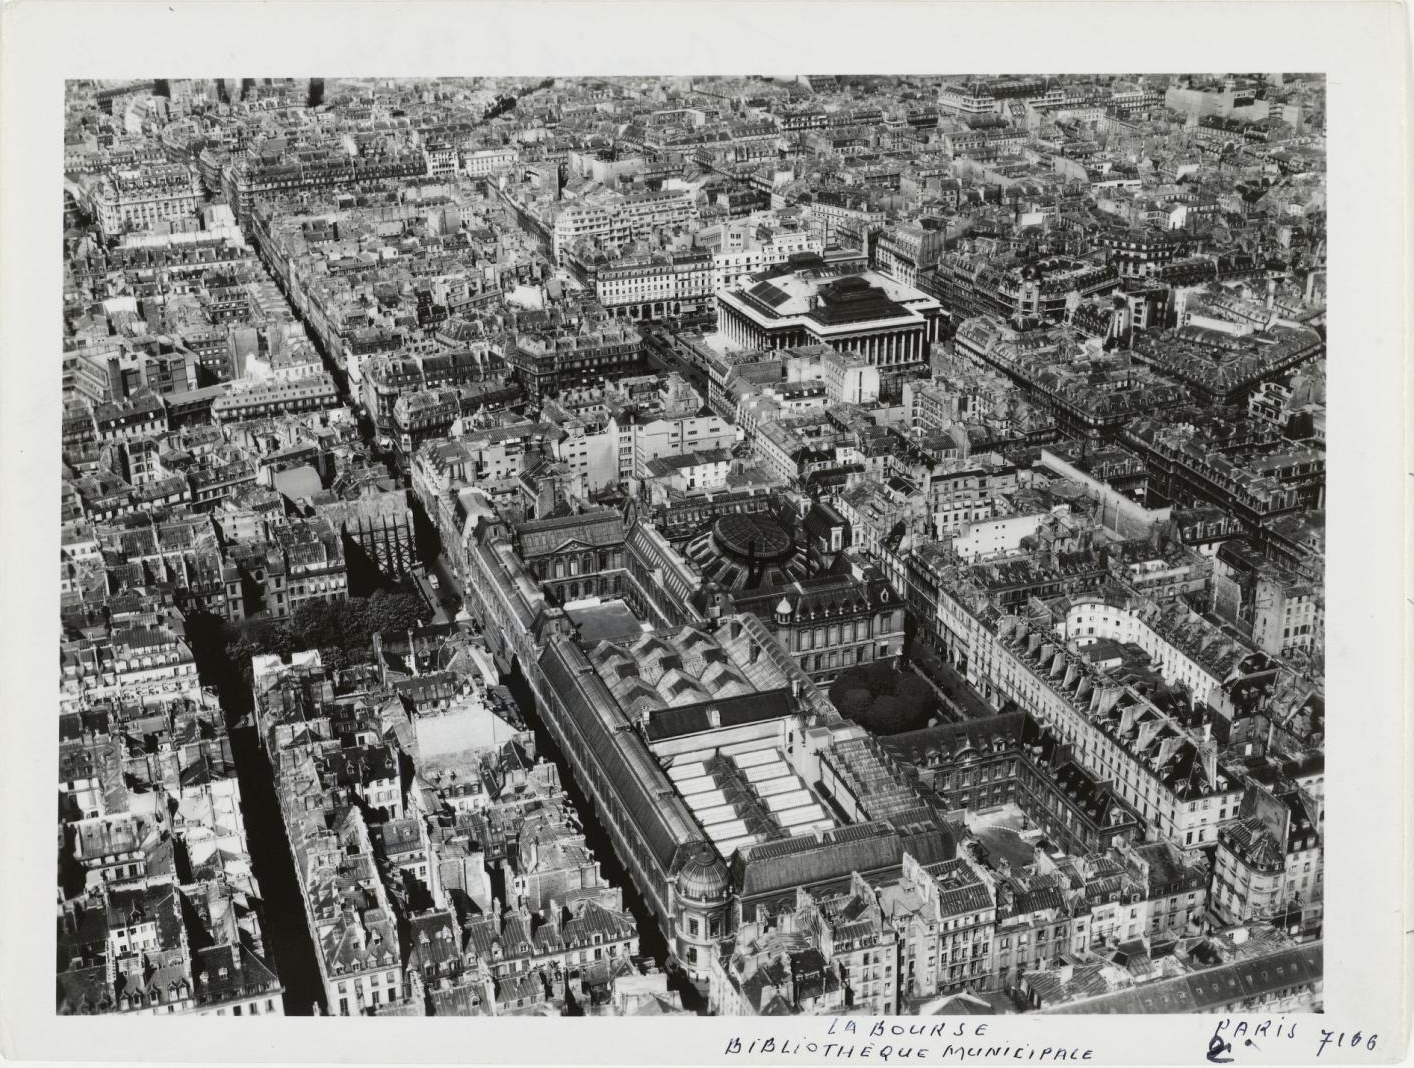
\includegraphics[width=1\linewidth]{images/vue_aerienne.png}
%     \caption{\href{https://www.parismuseescollections.paris.fr/fr/musee-carnavalet/oeuvres/vue-aerienne-de-paris-la-bourse-des-valeurs-palais-brongniart-et-la}{Vue aérienne de Paris} : la Bourse, le palais Brongniart et la Bibliothèque nationale, rue de Richelieu, Paris, Roger, photographie, 1952, Musée Carnavalet, PH344-7166.}
%     \label{fig:vue_aerienne}
% \end{figure}

\begin{table}[ht!]
\centering
\begin{tabular}{|l|c|c|}
\toprule
\textbf{Lieux de conservation} & \textbf{Nombre} & \textbf{Nombre} \\
\midrule
Musée Carnavalet & & 1333 \\
Bibliothèque nationale de France & 1312 & \\
Bibliothèques spécialisées de la Ville de Paris & 928 & \\
Bibliothèque historique de la Ville de Paris & 827 & \\
British Museum & 295 & \\
Institut national d'histoire de l'art & 162 & \\
Bibliothèque Forney & 73 & \\
Archives de Paris & 46 & \\
Palais Galliera & & 37 \\
Maison de Balzac & & 31 \\
Musée Albert Kahn & 30 & \\
Maison Victor Hugo & & 27 \\
Bibliothèque de l'Hôtel de Ville & 16 & \\
Bibliothèque Marguerite Durand & 5 & \\
Petit Palais. Musée des Beaux-Arts de la Ville de Paris & & 4 \\
Bibliothèque municipale et patrimoniale Villon & 4 & \\
Bibliothèque des littératures policières & 4 & \\
Musée de la Libération Leclerc Moulin & & 4 \\
Médiathèque Marguerite Duras & 2 & \\
Bibliothèque du tourisme et des voyages - Germaine Tillion & 2 & \\
Médiathèque musicale de Paris & 1 & \\
Musée de la Vie Romantique & & 1 \\
Musée Bourdelle & & 1 \\
\midrule
SOUS-TOTAL Paris Musées & & 1438 \\
\textbf{TOTAL} &  \textbf{5145} & \\
\bottomrule
\end{tabular}
\caption{Répartition du corpus iconographique par lieu de conservation}
\label{tab:iconographie_institution}
\end{table}

\newpage

Force est de constater que la numérisation partielle des collections par certaines institutions limite l'exhaustivité matérielle et historique d'un projet de recherche. Bien que la numérisation ait permis un accès inédit à une vaste quantité de documents, elle ne couvre qu'une portion des archives disponibles, laissant de côté des ressources certainement essentielles pour une constitution complète de l'histoire du quartier. Toutefois, cela est suffisant pour apporter un échantillon représentatif du quartier. Cette situation souligne non seulement les contraintes documentaires avec lesquelles le projet Richelieu s'est développé, mais elle constitue aussi un appel à élargir les chantiers de numérisation au sein des institutions patrimoniales, notamment pour le développement des bibliothèques numériques.\footnote{A titre d'exemple, l'ENC a pour ambition de numériser l'ensemble de ses archives et documents afin de créer une bibliothèque numérique. Le chantier, en fonction des financements, devrait être lancé à l'automne 2024.} 

\subsection{Les corpus secondaires}
\subsubsection{Le corpus textuel}
Ce corpus est principalement constitué de bottins, almanachs du commerce et anciens répertoires d'adresses. Ce type de publications proposant des listes d'adresses de commerçants, fabricants, industriels, etc. centrées sur un espace urbain donné est un genre en pleine expansion au XIX\ieme~  siècle. Ces ouvrages collectionnent et intègrent une masse d'informations qui ne cesse d'augmenter et de se diversifier tout au long de la période. Ils constituent aussi et surtout de véritables objets spatiaux et sociaux qui témoignent de l'évolution de la société. Les ensembles de références spatiales indirectes qu'ils contiennent (les adresses et localisations en tout genre) accompagnent et décrivent le développement des villes – notamment celle de Paris – , et l'augmentation de leur population. Ils exposent de manière fine les concentrations et les évolutions du commerce, de l'artisanat et de l'industrie, tout en témoignant de la société dans son ensemble. L'exploitation de ces informations de localisation en grand nombre constitue une source privilégiée pour étudier sur le long terme l'évolution des dynamiques sociales en contexte urbain, qui plus est à différentes échelles et niveaux d'observation et d'analyse. \footnote{L'étude est les méthodologies numériques d'analyse ont fait l'objet d'une journée d'études à la \acrshort{bnf} : \footcite{BNFJournee2022}}

Pour le projet Richelieu, le parti pris était de définir les métiers exercés dans le quartier. Les sources sont principalement issues de la \acrshort{bnf}. Au total, 56 annuaires datant de 1839 à 1922 ont été océrisé (\acrshort{ocr}) pour un volume considérable de données : 4 millions d'adresses dans tout Paris sont extraites des 27 000 pages. Nous verrons par la suite le devenir de ce corpus au sein du projet Richelieu dont le traitement et l'alignement des données en dépend. 

\subsubsection{Le modèle \acrshort{3d} historique}  
En complément des autres corpus, le projet a travaillé sur la constitution d'un modèle \acrshort{3d} historique. S'inspirant de projets analogues\footcite{GOUET-BRUNETIndexation2023a}, un relevé lasergrammétrique a été entrepris avec Plemo \acrshort{3d}. A partir de-là, et en inspiration au procédé photogrammétrique, le travail a consisté à replacer les vues représentatives d'un objet physique afin de montrer l'évolution architecturale à travers le temps. Ce travail s'est concentré sur la place de la Bourse au XIX\ieme~ siècle qui est aménagée sous le Premier Empire pour accueillir le Palais Brongniart à l'emplacement de l'ancien couvent des Filles-Saint-Thomas. Elle marque une étape décisive dans l'urbanisation du quartier : elle conditionne le prolongement de la rue Vivienne et devient un des épicentres économiques de la vie parisienne. Le travail s'appuie sur la collecte de 700 documents iconographiques (gravures, dessins, photos, plans) documentant l'évolution de la place entre 1810 et 1950. Un \acrlong{sig} (SIG) est utilisé pour spatialiser ces données dont les dimensions ne sont pas que la latitude et la longitude, sinon l'altitude et l'orientation de la prise de vue également. L'intégration de ce travail, à comprendre comme un modèle \acrshort{3d} enrichi de données historiques, au projet final est en cours d'interrogation. 

\subsubsection{Pour aller plus loin}
Reconstituer un quartier dans toutes ses dimensions est une entreprise ambitieuse. Pour ce faire, diverses sources peuvent enrichir l'analyse du quartier.

Les archives textuelles et administratives, telles que les permis de construire, les plans d'urbanisme, les recensements, les registres de propriété et les rapports municipaux constituent des sources d'informations pour l'étude du quartier. Les documents commerciaux et publicitaires, comme les annuaires et les guides, renseignent sur les activités économiques des commerces et entreprises, ainsi que sur l'évolution des habitudes de consommation. De plus, les registres de l'état civil et paroissiaux fournissent des données sur l'histoire démographique et permettent d'examiner les dynamiques familiales, sociales et sociologiques. Les articles de presse et les journaux constituent également une source précieuse : ils relatent des événements historiques et faits divers, présentent des annonces, des critiques et des témoignages sur l'histoire du quartier. La littérature, quant à elle, offre des perspectives subjectives mais souvent riches sur la vie quotidienne à travers des descriptions littéraires, des récits de voyageurs et des mémoires. Enfin, bien que sortant du cadre traditionnel de l'analyse documentaire, les éléments tels que le son, l'image animée, le film, ainsi que les sensations comme l'odeur et le goût de la ville moderne, peuvent également offrir des perceptions originales du quartier. Quelques unes de ces diverses pistes de réflexion ont animé les séminaires du projet et fournissent ainsi une multitude de perspectives sur le quartier à travers le temps.

\subsubsection{Conclusion}
En conclusion, l'exploration documentaire entreprise dans le cadre du projet Richelieu témoigne d'une ambition d'exhaustivité pour reconstituer l'histoire du quartier sur une période de deux siècles. La fouille des sources historiques, tant cartographiques qu'iconographiques, a permis de rassembler un ensemble de documents de natures différentes et essentiels pour visualiser l'évolution du quartier Richelieu. Cependant, la sélection des sources a été orientée par la contrainte de numérisation, limitant ainsi l'accès aux archives disponibles. Cette réalité met en lumière les défis liés à la recherche historique dans un contexte de numérisation partielle des collections. Finalement, la diversité des sources mobilisées, qu'elles soient cartographiques, iconographiques ou textuelles, enrichit considérablement la compréhension de l'histoire complexe et multifacette du quartier, offrant ainsi une approche multidimensionnelle et profondément ancrée dans le temps.


%%%%%%%%%%%%%%%%%%%%%%%%%%%%%%%%%%%%%
% SECTION %%%%%%%%%%%%%%%%%%%%%%%%%%%
\section{Définition des objectifs techniques}
Quels sont les objectifs du projet ? Que signifie pour les acteurs \enquote{investiger sur l'histoire de son quartier}? Comment cette investigation se concrétise-t-elle ?  Quelle forme prend-elle ? Quel est le développement informatique attendu ? Le but de cette sous-partie ici est de confronter les attentes initiales, telles que décrites dans les documents officiels, aux réalisations effectivement privilégiées afin de comprendre le moment dans lequel s'intègre le stage. Ce passage est réalisé à partir d'une étude comparative des appels à financements de projets de recherche auprès de la Fondation des sciences du Patrimoine qui distribuent de nombreux fonds\footnote{Pour plus d'informations, consulter la page : https://www.sciences-patrimoine.org/recherche/appel-a-projets/ }. 

Depuis le lancement du projet en 2018 jusqu'à sa finalisation prévue en 2024, l'objectif est demeuré constant : explorer les diverses dimensions de l'histoire du quartier (urbanistique, architecturale, économique, administrative, sociologique, culturelle) et concevoir un modèle innovant d'exploration des données patrimoniales à travers quatre axes principaux : le temps, l'espace, le réseau social, et l'iconographie. Comment se représenter cette innovation ? Les ingénieurs ont-ils accompagné les chercheurs pour cette définition ? Bien que cet objectif soit ambitieux, il reste clair. Un \enquote{système d'information innovant}\footcite{PROJETFondation2021} est souvent évoqué pour atteindre ce but, mais les détails techniques manquent dans l'appel à projet de 2021. Des concepts sont énumérés tels qu'un modèle conceptuel d'informations multidimensionnelles, l'ontologie \acrshort{cidoc}, le modèle de données d'annotation Web, le VIR, les représentations \acrshort{3d}, les informations cartographiques \acrshort{2d}, ainsi que l'intégration avec le Web de données et des autorités externes (Wikidata, Getty) sont mentionnés. De plus, l'exploration des données au format \acrshort{rdf} du Web sémantique à travers une plateforme utilisant \acrshort{sparql}, et l'implémentation d'Aïoli pour la plateforme \acrshort{3d}, sont également citées. 
Lors de l'appel à projet de 2023, le périmètre du projet a été redéfini et les ambitions sémantiques ont été remises en cause. Les objectifs sont le développement d'un outil d'exploration des données via une application Web servant d'\enquote{exposition finale des corpus du projet Richelieu}\footcite{PROJETFondation2023}. Une carte est d'ores et déjà attendue. Un catalogue iconographique l'est également. Le développement de cette application nécessite une chaîne robuste pour le traitement des données, qui sera présentée dans le chapitre suivant.

\subsubsection{Conclusion du chapitre}
Ce premier chapitre introductif a permis de poser le cadre du projet de recherche en présentant son contexte historique, son objet d'étude, ses acteurs, ses objectifs, ainsi que les corpus de recherche mobilisés. En inscrivant le projet Richelieu dans une démarche interdisciplinaire, il s'agit non seulement de comprendre l'émergence de l'archétype de la capitale moderne, et surtout de proposer une nouvelle clé de lecture du quartier Richelieu, en s'appuyant sur des collaborations nationales et internationales enrichissant l'écosystème de l' \acrshort{inha}. L'ambition du projet réside dans sa volonté de reconstituer l'histoire du quartier Richelieu sur une période de deux siècles, en utilisant une exploration documentaire et archivistique exhaustive. En dépit de ces contraintes, la diversité des sources mobilisées enrichit considérablement la compréhension du quartier Richelieu, offrant une perspective multidimensionnelle sur son histoire complexe. Le projet Richelieu, à travers le développement d'un outil d'exploration des données, se positionne comme une initiative pionnière pour approfondir notre connaissance de l'urbanisation parisienne et des dynamiques qui ont façonné ce quartier emblématique.
%%%%%%%%%%%%%% CHAPT 2 %%%%%%%%%%%%%%%%%%%%%%%%%%%%%%%%%%
\chapter{Contexte numérique : les états successifs de la donnée}
\chaptermark{Contexte numérique}
% PARTIE 1 - PRESENTATION %%%%%%%%%%%
% CHAPITRE 2 %%%%%%%%%%%%%%%%%%%%%%%%
%%%%%%%%%%%%%%%%%%%%%%%%%%%%%%%%%%%%%
Ce deuxième chapitre explore le cadre numérique dans lequel s'est développé le projet Richelieu, en se concentrant particulièrement sur le volet RICH.DATA II. Il détaille les différentes étapes de traitement des données, depuis leur saisie par les équipes du projet jusqu'à leur mise en ligne sur une application Web destinée au public. En général, le traitement des données consiste en une série de processus visant à extraire de l'information et du savoir à partir de données brutes, avec pour objectif de les rendre intelligibles par l'ordinateur plutôt que directement lisibles par l'humain. Nous examinerons ainsi les spécificités de la chaîne de traitement des données du projet Richelieu.

%%%%%%%%%%%%%%%%%%%%%%%%%%%%%%%%%%%%%
% SECTION %%%%%%%%%%%%%%%%%%%%%%%%%%%
\section{Saisir la donnée : un enjeu pour l'interaction \\chercheur-ingénieur}
Dans le projet Richelieu, la saisie des données est réalisée à la fois par les chercheurs et les ingénieurs, en fonction des corpus. L'objectif est de construire un système d'information multidimensionnel comprenant les axes principaux du projet, pour rappel, l'iconographique, l'espace, le temps et le réseau. Cette partie abordera en détails les traitements effectués sur les principaux corpus, iconographie et cartographie, tandis que les corpus secondaires ne seront pas abordés.

\subsection{Annotation, description et structuration du corpus iconographique}
Une image est souvent accompagnée d'une légende précisant son titre, son auteur, et parfois sa date de création, la technique utilisée, ses dimensions, et son propriétaire. Au musée, cette légende prend la forme d'un cartel où le numéro d'inventaire peut être ajouté. Dans une notice bibliographique, qu'elle soit imprimée ou publiée en ligne, cette légende inclut également le lieu ou site Web de publication, l'éditeur ou le laboratoire de recherche associé, ainsi que la pagination. Ces références bibliographiques suivent diverses normes et styles, parmi lesquels les formats Harvard et Chicago sont les plus connus. Que ce soit sous forme de légende, de cartel, de notice ou de référence bibliographique, cette information décrit l'image, constituant ainsi la première couche enrichie d'informations. En somme, c'est une donnée sur la donnée et c'est ce qu'on nomme une métadonnée. Dans notre cas, il s'agit de métadonnées descriptives et structurelles, mais il en existe une grande variété (administratives, contextuelles, techniques, statiques, évolutives, externes aux contenu, etc.). Le volume des métadonnées est proportionnel à l'ampleur du corpus réuni, et il est donc particulièrement conséquent pour le projet Richelieu car les dimensions d'études sont plurielles. Il est donc pertinent de se demander : quelles sont les métadonnées du projet ? Soit, comment le corpus iconographique devient une donnée computationnelle et comment est-elle structurée dans ce système d'information ?

\subsubsection{Méthodologie appliquée}
Les données sont saisies \enquote{manuellement}, sans extraction automatique des métadonnées. Les chercheurs remplissent minutieusement les fichiers au format xls, un format propriétaire de Microsoft Excel, en complétant case par case, ligne par ligne et colonne par colonne. Ces tableurs, hébergés en ligne sur le serveur de l'\acrshort{inha}, permettent une complétion simultanée par plusieurs chercheurs. Initialement, chaque zone géographique du quartier — Vivienne, Bourse, \acrlong{bdf}, Richelieu — disposait de son propre tableur. Dans chacun des tableurs, on retrouve un onglet, ou feuille, par institution, un onglet consacré aux lieux et un onglet documentant l'évolution des différentes adresses par lieu car les numéros de rue peuvent changer avec les modifications parcellaires. Les colonnes des tableurs sont composé de plusieurs champs intitulés comme suit :  \enquote{Institution}, \enquote{\textcolor{blue}{Identifiant interne}}, \enquote{Manifest IIIF}, \enquote{IIIF Folio}, \enquote{\acrshort{url}}, \enquote{Titre}, \enquote{Auteur 1}, \enquote{Auteur 2}, \enquote{Editeur}, \enquote{Date Institution}, \enquote{\textcolor{red}{{Date corrigée}}}, \enquote{Technique}, \enquote{N° d'inventaire}, \enquote{Corpus}, \enquote{\textcolor{red}{Description iconographique}},\enquote{Marques, inscriptions, poinçons}, \enquote{\textcolor{red}{Commentaire historique}}, \enquote{\textcolor{blue}{Thème(s)}}, \enquote{\textcolor{blue}{Entité nommée}}, {\enquote{\textcolor{blue}{Id localisation}}}, \enquote{\textcolor{red}{Note interne}}, \enquote{Document produit imprimé ou vendu dans le quartier}, \enquote{Représente la ville ou les marchandises}\footnote{La casse est respectée dans la transcription des intitulés de colonnes.} -- totalisant 24 niveaux d’information distincts pour chaque document iconographique. Ce qui représente 96 000 métadonnées descriptives rien que pour le corpus iconographique, pour rappel, constitué de 4000 documents. 

Les métadonnées ayant fait l'objet de recherches supplémentaires par les équipes sont indiquées en \textcolor{red}{rouge}. Il s'agit d'annotations et de descriptions absentes des données brutes. En \textcolor{blue}{bleu}, sont mises en évidence les métadonnées structurelles, qui organisent l'objet documentaire selon la logique du système d'information du projet Richelieu. Par exemple, \enquote{Id localisation} relie chaque iconographie à une adresse ou à des repères spatiaux, permettant ainsi de géolocaliser les éléments représentés, que ce soit des immeubles, des points de vue, ou des lieux d'événements. Par exemple, RV2 désigne le 2, rue Vivienne, RVA15 le 15, rue de Valois, GC26 le 26, de la galerie Colbert, et RR65 le 65, rue Richelieu. Les adresses évoluent toutefois au fil du temps : par exemple, l'actuel 2, rue Vivienne était répertorié comme 2 et 4, rue Vivienne selon l’Atlas Vasserot (1810-1836), puis comme 2 et 2bis, rue Vivienne dans les atlas de 1860 à 1900. L'une des tâches principales des chercheurs est de reconstituer cette évolution. Par ailleurs, la métadonnée \enquote{Date corrigée} permet d'élargir la perspective temporelle du projet, tandis que \enquote{Thème(s)} et \enquote{Entité nommée} multiplient les accès à l'information.

% Le numéro d'inventaire dont nous avons cité en introduction de ce chapitre est plus exactement à considérer comme une métadonnée structurelle : il classifie l'œuvre selon un ordre ou une hiérarchie. Par exemple, le numéro d'inventaire \href{https://www.navigart.fr/picassoparis/artwork/pablo-picasso-autoportrait-160000000000541?page=1&filters=query%3AMP4}{MP4} signifie qu'il s'agit de la quatrième œuvre inventoriée lors de la succession Picasso pour la constitution du Musée national Picasso-Paris (MnPP). Tandis que le numéro d'inventaire \href{https://www.navigart.fr/picassoparis/artwork/pablo-picasso-portrait-d-olga-160000000001246?page=3&filters=tree_domain_all%3ADessin,,year%3A1921__1933}{MP1990-70} est la 70eme œuvre inventoriée en 1990 lors de la dation de Jacqueline Picasso pour le MnPP. Le projet Richelieu a également inventorier chaque document de son corpus : un identifiant unique lui est décerné. 

\subsubsection{Méthodologie recommandée}
Cependant, il est recommandé de contraindre la saisie des données par des règles, notamment pour assurer leur qualité. Laisser libre l'écriture avec majuscules, minuscules, espaces, signes de ponctuation, abréviations ou fautes de frappe augmente le risque d'erreur au lieu de le réduire. Comment garantir l'homogénéité et la qualité pour un volume important des données sans un cadre rigoureux ? L'outil utilisé dans le projet, Excel, propose un système de validation des données qui permet de définir divers critères, comme l'utilisation de masques de saisie pour restreindre les entrées. Il existe de nombreuses bonnes pratiques pour la saisie et la validation des données brutes, mais leur application dépend encore du contexte.

\subsubsection{Difficultés contextuelles}
En effet, ces contraintes deviennent difficiles à appliquer lorsque l'ingénieur intervient après qu'un premier travail de fouille, d'annotation, et de description des données ait été réalisé par les chercheurs, autrement dit par les équipes se succédant. De plus, le corpus se construit simultanément à sa description et à sa saisie. Le dépouillement d'un fonds, puis d'un autre, révèle des métadonnées descriptives intéressantes qui peuvent être absentes dans les collections déjà décrites. Une institution peut indiquer les multiples auteurs d'une œuvre alors qu'une institution se limitera à l'auteur principal. Ainsi, les métadonnées peuvent être enrichies par une collection, mais aussi entraîner un appauvrissement des informations pour une autre.

\subsubsection{Le rôle des standards et normes (ontologies, index, thésaurus)}
Pour surmonter certaines difficultés rencontrées lors de la saisie, on pourrait se demander : est-il possible d'extraire automatiquement les métadonnées à partir des bibliothèques numérisées ? Peut-on appliquer des normes et standards numériques dans le cadre du projet Richelieu pour faciliter la saisie ? L'extraction automatique n'est pas toujours à privilégier en raison de la diversité des structures de données utilisées par les bibliothèques et catalogues du musées numérisés. Ce constat s'explique par le fait que les institutions ne structurent pas leurs données de manière uniforme, même lorsqu'il existe des standards et des normes. Les ontologies, thésaurus, et index jouent un rôle structurant en fournissant des cadres normalisés pour harmoniser les données. Ces outils facilitent la recherche, l'interopérabilité, et l'exploitation des informations. Par exemple, il est recommandé aux institutions patrimoniales relevant des Musées de France de suivre les règles de l'export Joconde\footcite{MINISTEREDELACULTUREJoconde2024}. Pourtant, l'application de ces normes n'est pas obligatoire, et certaines institutions les adaptent tandis que d'autres ne les utilisent pas du tout tels que certains musées réunis sous l'établissement Paris Musées. En conséquence, les métadonnées descriptives varient considérablement d'une institution à l'autre, rendant l'harmonisation et l'extraction automatique plus difficile et questionnant la pérennité des données non standardisées. Enfin, malgré sa nature fastidieuse, la saisie manuelle reste une étape nécessaire voire indispensable pour garantir un contrôle qualité. Adopter des normes et standards dépend donc de la compatibilité avec les systèmes existants et des ressources (humaines et techniques) disponibles. Surtout, l'extraction est utile quand le corpus est bien identifié à l'inverse de celui du projet Richelieu qui l'a constitué au fur-et-à-mesure de la recherche. De plus, dans certains projets, notamment ceux ayant un objet central spécifique et un délai restreint, comme c'est le cas du projet Richelieu, il semble plus efficace de créer une grammaire de structuration des données sur-mesure plutôt que de tenter d'appliquer des standards externes. 


\subsubsection{Les formats d'entrée}
La saisie du corpus iconographique n'adhère pas à une norme standardisée de description des métadonnées. Toutefois, cette étape permet à l'ingénieur de produire un document au format conventionnel pour le traitement, tel que le \acrshort{csv}. Faisons remarquer que le corpus iconographique ne se compose pas de fichiers d'images tels que \acrshort{png}, \acrshort{jpg}, \acrshort{tiff} ou \acrshort{svg}. Au lieu de cela, il s'agit principalement d'\acrshort{url} (\textit{Uniform Resource Locator}), qui sont considérées comme des métadonnées à part entière. Ces \acrshort{url}, suivant le protocole \acrshort{iiif} (\textit{International Image Interoperability Framework}), offrent des avantages spécifiques, de volume et d'intéropérabilité des données sur le Web, que nous aborderons plus tard (voir le chapitre \ref{section:intero}). 

%%%%%%%%%%%%%%%%%%%%%%%%%%%%%%%%%%%%%
\subsection{Géoréférencement historique du corpus cartographique}
La numérisation des données cartographiques s'effectue par l'ingénieur en étroite collaboration avec l'équipe de chercheurs pour saisir et traiter ces informations. 

Pour rappel, une carte est une représentation à échelle réduite de la surface terrestre, et dans le cas du quartier Richelieu, cette réduction est particulièrement importante. Les cartes sont souvent accompagnées d'un graticule, une grille de lignes représentant un système de coordonnées géographiques. Pour se localiser sur une carte, on utilise un système de coordonnées composé d'un ensemble de repères constitués de points et lignes imaginaires : les pôles Nord et Sud, l'Équateur et ses parallèles alors croisés perpendiculairement par les méridiens. Une position géographique est le point d'intersection de deux de ces lignes, correspondant respectivement à la latitude (x) et à la longitude (y). L'une est déterminée par rapport à un méridien et l'autre par rapport à un parallèle. Parfois, une troisième dimension, l'altitude (z), est également considérée, elle est calculée vis-à-vis du niveau moyen de la mer. Aujourd'hui, la géolocalisation ou géopositionnement est  rapidement calculé par divers systèmes de navigation comme le \acrshort{gps} (états-unien), Glonass (russe), Galileo (européen), et Beidou (chinois). Dans le contexte de la numérisation de cartes et plans, les outils que manipule l'équipe, tel que \acrshort{qgis}, se base sur le \acrshort{gps} pour intégrer les données géographiques dans un plan en \acrshort{2d} qui applique une projection géodésique\footcite{GEOCONFLUENCESProjection2022} en Lambert 93. C'est sur cette base informatisée que le géoréférencement historique peut être effectué.


\subsubsection{\textit{Ti esti} le géoréférencement ... historique ?}
Le géoréférencement\footcite{GEOCONFLUENCESGeoreferencement2024} est un principe fondamental de la cartographie assistée par ordinateur (\acrshort{cao}). Il consiste à déterminer la position dans l'espace d'un objet en utilisant les données d'un système de coordonnées. L'objet n'a pas de coordonnées connues et le système de coordonnées permet de lui en donner. En l'occurrence, un plan historique de la ville de Paris est dépourvu de coordonnées informatiques. Si on le place sur une carte contemporaine numérisée, il se peut que tel mur de tel édifice patrimonial ne coïncide pas avec le même mur sur la carte contemporaine. Pour assurer une cohérence, on créé des points de contrôle, aussi appelées géoréférences, qui sont l'équivalent des éléments géographiques représentés sur les plans. Cette technique permet d'ajuster la carte à une projection choisie ou de changer d'échelle, ce qui est une opération courante dans le \acrlong{sig} (SIG)\footcite{BERNIERconcepts2014} dans lequel l'objet, la carte est un fichier raster (une image composée de pixels) et les coordonnées sont des objets vectoriels (des points, lignes, polylignes, polygones représentant les objets physiques). 

Mais qu'est-ce qu'une géoréférence historique, également appelée référentiel historique ? Aujourd'hui, la dimension géographique est de plus en plus intégrée dans les recherches en histoire, archéologie, et histoire de l'art, via la cartographie des territoires étudiés\footcite{ZOHARGeographic2022, TIMARWeb2024}. Le partage entre les communautés de chercheurs des éléments structurants l’espace géographique à différentes époques de temps, permet de gagner un temps précieux et est devenu une pratique courante. Ces éléments communs sont ce que l'on appelle un \enquote{référentiel géohistorique}. C’est l’un des objectifs majeurs du \acrshort{cstptm} que de constituer ces références géographiques et historiques afin d'en faciliter l’accès et l’usage. C’est en ce sens qu’un travail important a été engagé par le \acrshort{cstptm} sur le plan 1900 de Paris qu'exploite le projet Richelieu.

\subsubsection{Outils et méthodes}\label{par:méthodes}
Dans le cadre du projet Richelieu, l'équipe utilise principalement la méthode de géoréférencement par points de contrôle, une technique manuelle qui demande une grande précision. Cette méthode est appliquée aussi bien dans \acrshort{qgis} que dans l'outil \acrshort{galligeo}. 

\acrshort{qgis}, un logiciel libre de \acrshort{sig}, permet de créer des cartes géographiques et de gérer des données spatiales basées sur un modèle d'information géographique constitué de couches provenant de sources diverses. \acrshort{qgis} prend en charge les formats standardisés pour l'information géographique, y compris les fichiers raster\footnote{Un raster est une grille appelée matrice composée de cellules organisées en ligne et en colonne. Chaque celllule est un pixel unique. Chaque pixel a des valeurs, de couleurs par exemple. L'association de l'ensemble des pixels crée une image. Plus communément, si on zoom sur cette image et qu'elle est pixelisée car la netteté se dégrade, c'est alors un raster.} et vectoriels\footnote{Un fichier vectoriel n'est pas composé de pixels mais contient des attributs (les informations descriptives qui lui sont associées) et une géométrie (sa forme créée de point, ligne et polygone)}. En résumé, un fichier raster est une image composée de pixels, tandis qu'un fichier vectoriel représente des objets physiques par des points, lignes, et polygones alors calculables par l'ordinateur. C'est pourquoi les données raster, bien que plus complexes à analyser, sont souvent utilisées comme fonds de cartes, sur lesquelles des données vectorielles sont superposées. C'est une image que l'on vient enrichir d'informations. Cependant, bien que \acrshort{qgis} dispose d'un module intégré pour le géoréférencement, appliquer cette technique à des plans historiques peut s'avérer complexe en raison de l'absence de graticules nécessaires pour un géoréférencement absolu, rendant le géoréférencement historique relatif.

Le projet Richelieu enrichit les fonds de cartes historiques en intégrant des informations sur l'évolution du tissu urbain, informatisées sous forme de polygones représentant l'emprise au sol des bâtiments. Chaque polygone est associé à des coordonnées géographiques (x et y) et une clé d'identification, et le travail finalisé est sauvegardé au format \textit{shapefile}. Les fichiers raster utilisés initialement sont généralement au format \acrshort{geotif}, robuste et polyvalent. Pour créer ces fichiers, l'équipe utilise la plateforme \acrshort{galligeo}, développée par Eric Mermet du Pôle géomatique\footcite{ALPAGEGlossaire2024} de l’\acrshort{ehess} (membre fondateur du \acrshort{cstptm}). \acrshort{galligeo} applique des méthodes similaires de géoréférencement par points de contrôle pour des cartes anciennes disponibles sur Gallica, la bibliothèque numérique de la \acrshort{bnf}. Cet outil en ligne récupère l’\acrshort{url} de la carte-image sur Gallica, puis l'utilisateur identifie des points homologues sur l'image et sur des cartes contemporaines déjà géoréférencées. Ce processus se déroule en flux de données, sans téléchargement, permettant aux utilisateurs de constituer une collection de cartes géoréférencées accessibles en ligne via un \acrshort{sig}. Ce flux de données, déjà utilisé dans le projet \acrshort{anr} ALEGORIA\footcite{ENSG-GEOMATIQUEIGNProjet2022} pour des fonds iconographiques, est particulièrement innovant dans le contexte des cartes historiques.

Une autre méthode utilisée pour le géoréférencement est la méthode dite \enquote{régressive}. Celle-ci repose sur un plan vectoriel actuel des îlots, du réseau des voies et des adresses. Le processus commence par l'identification des éléments qui n'ont pas changé depuis une date précise, comme 1900. Ensuite, des corrections mineures sont apportées aux objets ayant subi de légères modifications, et ceux qui ont disparu ou ont été profondément transformés sont reconstitués. Cette approche réduit considérablement le travail de saisie, permettant de gagner un temps précieux, et facilite la superposition des cartes anciennes successives jusqu'à aujourd'hui, en identifiant les changements par rapport aux éléments constants. Grâce à cette méthode, divers procédés ont été développés pour gérer les \enquote{créations, disparitions et transformations}, permettant ainsi aux acteurs du \acrshort{cstptm} de reconstituer environ 5 000 îlots de 1900 à partir des quelque 7 500 îlots actuels, 3 900 voies de 1900 à partir des 6 000 actuelles, 17 000 tronçons de voies de 1900 à partir des 36 000 actuels, et enfin 118 700 points d’adresse de 1900 à partir des 150 000 actuels sur tout Paris. 

L'alignement des cartes anciennes avec la topographie actuelle nécessite l'utilisation de divers outils et méthodes développés par un large réseau, mettant en lumière l'importance de l'interdisciplinarité. La collaboration étroite entre chercheurs et ingénieurs exige une adaptation mutuelle, alliant les contraintes de l’ingénierie numérique et documentaire aux exigences scientifiques de l’histoire du tissu urbain, pour atteindre un objectif commun : la spatialisation des données historiques.

% \subsection{Le corpus textuel par extraction}
% La donnée du corpus textuel est extraite par océrisation. Ces documents écrits possèdent la même structure : 3 colonnes, dont chacune est censé recenser la même information. Chacune des colonne représente un segment à océriser, soit une image unique par colonne. L'outil de segementation des images utilisé est dhSegment \note[MC]{Mettre un lien vers cet outil, ou le décrire rapidement}. Sur un modèle de 90 pages segmentées à la main, 27 000 pages ont ainsi pu être segmentées. Concernant l'OCR, l'outil de Google Cloud Vision a été privilégié car il semblerait que les chiffres soient plus facilement lisibles \note[MC]{Dans l'idéal, il faudrait le justifier avec certitude (mais cela est sûrement compliqué dans ton cas si tu n'as pas participé aux études sur GCV): un lien vers une étude, vers une annexe, ou bien un tableau des comparaisons qui ont amené à ce choix.}. Puis, un premier alignement de ces deux jeux de données a été effectué. Mais, sur les 4 millions de lignes, seules un très faible pourcentage de ce traitement obtient un bon score de lisibilité. La troisième colonne n'enregistre pas les données de façon uniforme. C'est pourquoi seules 1000 lignes constituent le corpus textuel du projet Richelieu une fois traité. 

% %%%%%%%%%%%%%%%%%%%%%%%%%%%%%%%%%%%%%
% \subsection{Les corpus secondaires}
% \subsubsection{Le corpus photogrammétrique}
% Une spatialisation des points de vue depuis lesquels la Place de la Bourse est représentée dans notre corpus iconographie => cf multidimensionnalité du projet de F. Clavaud. Un exemple d'ontologie descriptives : RICO et les données géographiques. 
% \note[MH]{Intégrer screen des différentes prises de point de vue des photos}

\subsubsection{Conclusion}
La saisie de la donnée est un processus particulièrement long pour les équipes du projet Richelieu qui a su faire appel à divers outils et méthodes reflétant les ambitions d'exhaustivité du système d'information géolocalisé. Mais elle ne constitue que la première étape de la chaîne de traitement, la modélisation de la donnée étant la suivante.

%%%%%%%%%%%%%%%%%%%%%%%%%%%%%%%%%%%%%
% SECTION %%%%%%%%%%%%%%%%%%%%%%%%%%%
\section{Modéliser la donnée : le lieu comme objet central}
La modélisation des données est une étape essentielle pour l'intégration en base de données. Ce processus consiste à créer une représentation d'un domaine de connaissances, ou d'un objet réel, sous la forme d'une structure de données dont les relations sont clairement définies pour ensuite être étudiées, manipulées et comprises\footcite{FLANDERSShape2018}. Il s'agit de formaliser la logique du système pour identifier les éléments constitutifs, ainsi que leurs similitudes et différences. Cette étape permet également de structurer les enjeux de recherche du projet et d'y répondre par une modélisation qui envisage les corpus sous un angle commun et précis\footcite{SOUTOUModelisation2017}. Présenter et maîtriser les subtilités du modèle de données est une étape nécessaire pour préparer leur exposition sur une application. Dans le cadre du projet Richelieu, la question clé est : comment relier les différents corpus qui le composent ? Quelles sont leurs relations, leurs points communs et leurs différences ? Les exigences spatiales des données documentaires ont fortement influencé la réflexion et la définition du modèle de données du projet. Il est important de noter que plusieurs niveaux de modélisations informatiques existent : conceptuel, logique et physique - parmi lesquelles nous aborderons la modélisation conceptuelle qui présente les entités, les types et les relations définies, et, la modélisation physique pour son implémentation en SQl. 

\subsection{Le modèle conceptuel : le lieu comme entité centrale.}

Le modèle conceptuel de données consiste à représenter visuellement et de façon simplifiée la structure des données d'un système d'information. Pour ce faire, et, dans le cadre du projet Richelieu, on se demande comment modéliser la notion d'espace entre les différents corpus ? Pour y parvenir, le projet a dû surmonter plusieurs contraintes logiques, explorant diverses modélisations avant de converger vers la notion de lieu\footcite{KERVEGANmarque2023}. Par exemple, l'adresse a été envisagée comme entité centrale, mais cela ne permettait pas de représenter l'évolution du tissu urbain, comme dans le cas du 2, rue Vivienne, évoqué précédemment. Une autre approche consistait à utiliser les coordonnées géographiques (x, y) comme point de référence, une méthode couramment appliquée dans des projets similaires. Cependant, ce modèle présentait des problèmes logiques liés à l'échelle réduite du quartier : où placer précisément le point sur un édifice — sur la façade, à l'arrière, dans la cour, etc. ? De plus, cette solution ne répondait pas aux enjeux scientifiques du projet, qui se concentrent sur la réalité bâtie.

Ainsi, la modélisation par le lieu s'est révélée être une approche plus appropriée compte tenu de la masse de données à traiter :
\begin{displayquote}{\enquote{La chaîne de traitement mise au point pour le projet est définie autour d'un objet central : le lieu. Cette entité, définie dans le temps et dans l’espace, et représentée par des ressources iconographiques et cartographiques. Elle est également un espace de vie, habité et pratiqué. Le lieu est donc capable de croiser les composantes spatiales, architecturales, socio-économiques, historiques et culturelles du quartier. C’est un objet qui permet de faire dialoguer les différents corpus et d’étudier la spatialité du quartier ; c’est donc autour de lui que la chaîne de traitement a été développée.}}\footcite{PROJETFondation2023} 
\end{displayquote}

Le lieu, en tant qu'entité centrale, permet de décloisonner les corpus spécialisés et devient le socle commun pour un ensemble d'informations, jouant un rôle clé dans les opérations de géoréférencement. 

\begin{figure}
    \centering
    \includegraphics[width=1\linewidth]{images/modèle_conceptuel2.png}
    \caption{Modèle conceptuel du projet Richelieu, Paul Kervegan, 2023.}
    \label{fig:enter-label}
\end{figure}

\subsection{Le modèle physique de la base de données relationnelle.}\label{sous-section:modele-bddr}
La modélisation physique est une étape capitale qui précède l'implémentation des données dans un système de gestion de base de données. Pour le projet Richelieu, cela se traduit par l'utilisation d'une base de données relationnelle (\acrshort{bddr}), où les données sont structurées en tables (similaires à des tableurs), composées de champs (équivalents aux intitulés de colonnes). Ces tables sont interconnectées par des relations, toujours établies via des clés primaires et étrangères. Une clé étrangère dans une \acrshort{bddr} est un champ qui établit un lien entre deux tables en faisant référence à la clé primaire d'une autre table. Elle garantit l'intégrité référentielle car elle s'assure que la valeur existe dans la table correspondante. Une \acrshort{bddr} permet de réaliser des requêtes complexes pour manipuler et interroger les données de manière efficace. Le modèle physique du projet Richelieu est d'une complexité relative, comme en témoigne la représentation graphique \ref{fig:modele-physique-bdd}.
\begin{figure}
    \centering
    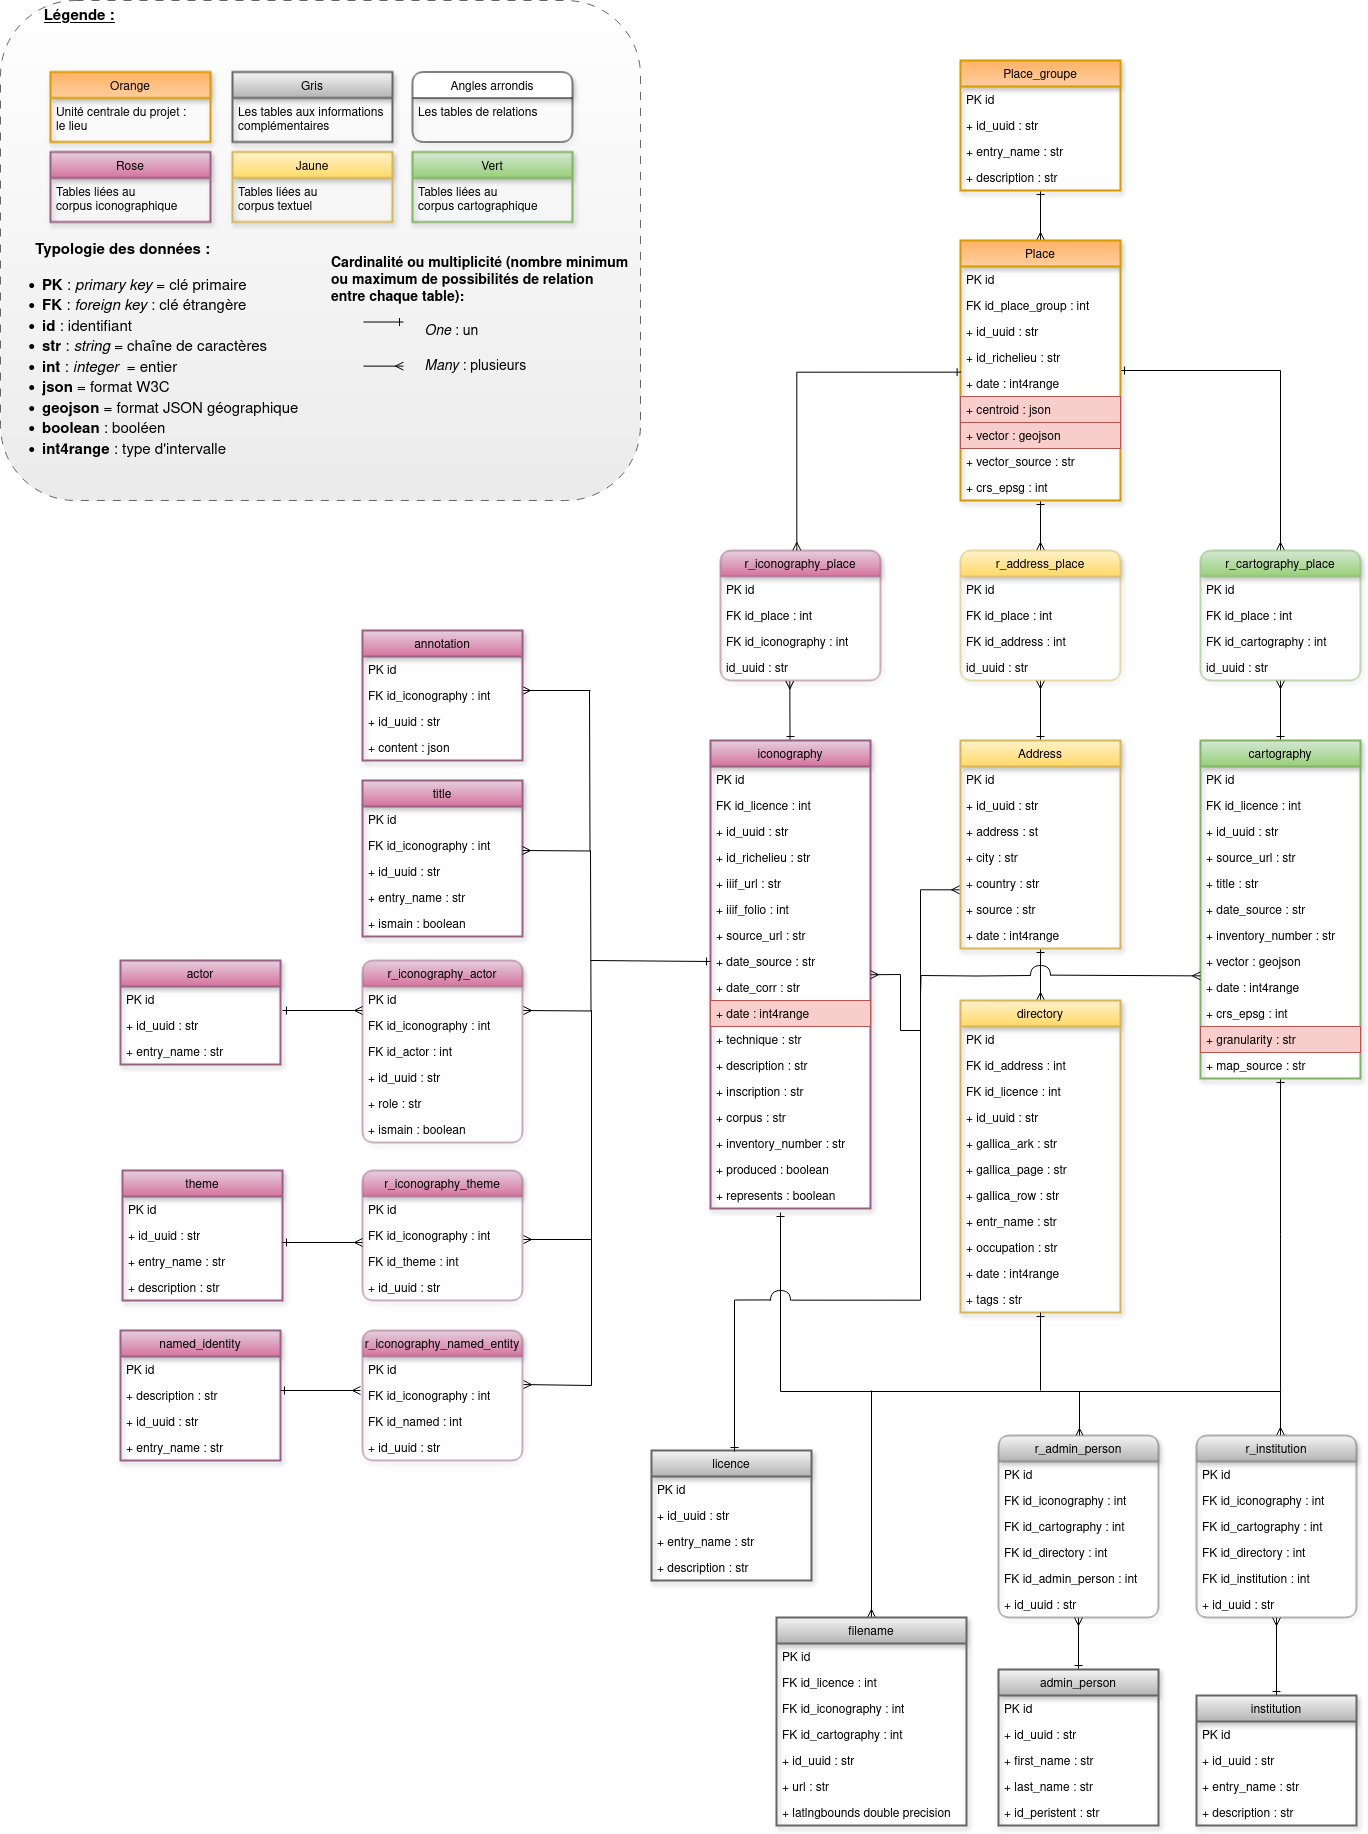
\includegraphics[width=1\linewidth]{images/modele-physique-bddr.drawio.png}
    \caption{Modèle physique des données du projet Richelieu, \mhd.}
    \label{fig:modele-physique-bdd}
\end{figure}

Examinons la structure du modèle dans ses grandes lignes. Ce modèle est organisé en plusieurs entités principales, chacune représentant une table dans la base de données. Au total, le modèle comprend 23 tables, regroupées par catégories fonctionnelles et différenciées par des couleurs spécifiques (par exemple, les tables en rose pour le corpus iconographique et celles en gris pour les informations administratives et descriptives reliées à l'ensemble des corpus). Chaque table possède une clé primaire (\acrshort{pk} : \textit{Primary Key}) qui permet d’identifier de manière unique chaque enregistrement. De nombreuses tables comportent également des clés étrangères (\acrshort{fk} : \textit{Foreign Key}) pour établir les relations entre elles, renforçant ainsi l'intégrité référentielle du modèle. Ainsi il y a 8 tables de relations, mais certaines relations se font en dehors de ces tables. Elles sont soit de type \enquote{un à plusieurs} soit \enquote{plusieurs à un}, comme l'indiquent les lignes connectant les tables. Elles sont essentielles pour maintenir la cohérence des données et permettre des jointures efficaces lors des requêtes. Par exemple, un lieu peut être associé à plusieurs documents iconographiques, cartographiques ou textuels, tandis qu'une licence spécifique peut s’appliquer à plusieurs sources documentaires.

Chaque table est constituée de divers champs, tels que des chaînes de caractères, des entiers ou des booléens, permettant de stocker une gamme variée d'informations comme des identifiants, des descriptions textuelles, des dates et des attributs spécifiques à la donnée spatiale. En plus des clés, le modèle comprend ainsi 85 attributs (les champs) qui structurent la diversité des informations. La définition des types de données est une étape importante pour assurer qu'elles respectent une qualité, une cohérence et une certaine forme d'intégrité. Le modèle présente également des associations complexes entre les tables, telles que celles entre \enquote{iconography} et \enquote{cartography}, soulignant l'interconnexion des données, comme le prévoyait le modèle conceptuel. On observe que la modélisation est pyramidale, avec toutes les informations convergeant via la table \enquote{place}, le lieu. En résumé, le modèle contient environ 30 000 lignes de données, sans compter les tables de relations, et plus de 104 000 données en incluant ces dernières. Le volume de données peut paraître moins conséquent que d'autres projets de recherche analogues, mais répartir ce volume à l'échelle du quartier est assez conséquent. On peut espérer que le modèle répond aux exigences pour la gestion d'un corpus de données riche, varié, complexe et multidimensionnel.

Nous avons mis en évidence en rouge certains enregistrements qui soulignent les particularités du modèle. Dans la table \enquote{cartography}, le champ \enquote{granularity} indique le niveau de détail ou de précision des données cartographiques. La granularité est classée en cinq catégories : \enquote{ensemble}, \enquote{aile}, \enquote{galerie}, \enquote{parcelle} et \enquote{point}, chacune correspondant à une échelle de représentation du quartier. Par exemple, le Palais Royal est étudié comme un ensemble architectural, mais ses différentes ailes (Beaujolais, Montpensier, Valois) et galeries (galerie de Bois devenue galerie d'Orléans) sont également détaillées. Cette granularité reflète la diversité de la réalité bâtie du quartier Richelieu.
Nous notons que la date est souvent enregistrée, mais avec plusieurs typologies attribuées. Dans la table \enquote{iconography}, un travail approfondi de datation des sources iconographiques a été réalisé par l'équipe de recherche. De nombreuses incohérences temporelles ont été constatées dans les notices des documents, conduisant à une correction manuelle et à la création d'une typologie spécifique. Lorsqu'une date précise est inconnue ou erronée, un intervalle de dates est utilisé plutôt qu'une date unique. Ce type de données permet de stocker des plages de dates dans une seule colonne de manière compacte, bien que le type \enquote{daterange} existe et aurait pu être une alternative.
Enfin, examinons les données de la table \enquote{place}, où les champs \enquote{centroid} et \enquote{vector} utilisent des structures de données incluant des informations géographiques, telles qu'un polygone qui a pour valeur des coordonnées géographiques (x,y). Le format \acrshort{geojson}, basé sur un système de \enquote{clé~:~valeur}, est particulièrement adapté pour stocker ces données complexes qui sont difficiles à représenter dans des colonnes traditionnelles\footcite{Definition2024}. Ce format est donc très utile pour les applications nécessitant des informations géospatiales, comme c'est le cas pour le projet Richelieu.

Ainsi, la granularité, les dates, les vecteurs et la richesse des données iconographiques correspondent aux dimensions que le projet souhaite modéliser : l'espace, le temps et l'iconographie. Cependant, la dimension du réseau semble être implicite dans le modèle, à moins qu'elle ne soit représentée par le nombre d'interconnexions présentes. Une analyse plus approfondie du contenu de la base de données permettra de clarifier cette question, ce qui sera exploré dans la prochaine partie.

En conclusion, il est évident que la modélisation constitue une étape fondamentale. Sans elle, la modularisation du lieu et l'identification de certains avantages n'auraient pas été possibles. Elle permet de décomposer la complexité en fragments plus simples, de diviser l'objet principal en objets secondaires pour une gestion autonome, tout en préservant les connexions nécessaires entre ces objets grâce au modèle de données relationnel.

%%%%%%%%%%%%%%%%%%%%%%%%%%%%%%%%%%%%%
% SECTION %%%%%%%%%%%%%%%%%%%%%%%%%%%
\section{Encoder pour stocker la donnée}
Définir la modélisation d'une base de données et les types à respecter ne suffit pas à la créer, il faut encore l'encoder afin de préparer son stockage dans un système de gestion de base de données. Cette étape est le cœur du traitement de la donnée, le \enquote{\textit{data cleaning}} (nettoyage des données) et le \enquote{\textit{data formatting}} (formatage des données) peuvent alors être effectué.

\subsection{\textit{Data Cleaning}}
Le nettoyage des données cherche à réduire le pourcentage d'erreurs suite à la saisie, réduire le \enquote{bruit} environnant les données. Cette étape a ainsi pour but d'assurer la qualité des données afin que celles-ci respectent les contraintes et règles définies, assurant aussi leur harmonisation. Cette étape est d'autant plus essentielle lorsque les données sont saisies manuellement. 

Dans le projet Richelieu, le nettoyage des données est une tâche considérable. Il faut d'abord s'assurer de nettoyer les tableurs en supprimant les en-têtes des colonnes et les colonnes vides à la fin des fichiers. Le nettoyage automatique, bien que précis, rencontre des difficultés pour corriger les fautes de frappe, gérer les valeurs manquantes, les doublons, et respecter la casse. Cela souligne l'importance de définir des règles strictes dès la saisie des données.

Cependant, l'équipe ingénieur-chercheur a trouvé des solutions pour surmonter certains problèmes de saisie : l'utilisation du \textit{pipe} ( | ) comme séparateur d'informations pour le traitement des entités nommées et des thèmes a permis de ne pas multiplier les colonnes à traiter, et d'éviter d'utiliser la virgule dont un traitement aurait été compliqué, au vue de son utilisation importante dans les autres cases du tableur. Le nettoyage principal se concentre sur la concaténation des fichiers pour qu'ils deviennent d'abord des jeux de données séparés puis formant un seul \textit{dataset}, tout en veillant à ce que les jointures entre les corpus soient possibles. Ensuite, des scripts Python sont développés pour associer les lignes aux fichiers image et vérifier qu'il n'y a pas de manque - auquel cas ils sont répertoriés dans un fichier annexe à destination des chercheurs qui doivent alors le compléter. Ce fichier est ensuite de nouveau traité pour être intégré au \textit{dataset} général. La conversion des fichiers (shapefiles en DataFrame ou \acrshort{geojson}, \acrshort{geotif} en \acrshort{png}) et l'harmonisation des coordonnées géographiques en EPSG:3857 / WGS84, le système de coordonnées cartésien utilisé par la bibliothèque JavaScript pour le développement de la carte, sont également effectuées. Nettoyer autant que possible garantit des données valides et facilite leur gestion par le système de base de données.

\subsection{\textit{Data Formatting}}
Après le nettoyage, vient l'étape du formatage des données, qui vise à rendre ces dernières compréhensibles pour l'ordinateur. Cela implique de standardiser les formats en adaptant les données aux exigences spécifiques de la base de données, et de s'assurer que les types de données sont corrects (par exemple, qu'un décimal n'est pas stocké comme un entier). Un travail particulier a été réalisé sur la normalisation des dates en utilisant le type \enquote{int4range}. La structuration du \textit{dataset} consiste ensuite à organiser les informations pour qu'elles correspondent à la structure des tables du modèle physique. Les quatre tables principales (iconographie, cartographie, textes, et lieux) sont traitées distinctement grâce à la librairie Pandas du langage de programmation Python.

Un aspect à relever de cette étape est la génération d'un système d'identification double pour chaque enregistrement de la donnée. D'une part, des clés primaires et étrangères sont créées pour chaque enregistrement. Même s'il ne s'agit pas d'identifiant à proprement parlé, les clés permettent toutefois d'identifier les données et sont essentielles pour le fonctionnement interne de la base de données, pour assurer la connexion entre les différentes tables. Les clés sont invisibles par le public. D'autre part, un \textit{Universal Unique Identifier} (\acrshort{uuid}) est généré pour chaque entrée. Ce code unique à 128 bits, composé de 36 caractères organisés en 5 groupes séparés par des tirets (8-4-4-4-12), garantit l'unicité de chaque enregistrement, même s'il est créé dans des environnements différents, à savoir dans plusieurs \textit{dataset}. Ce format est globalement unique, indépendant et sécurisé. Enfin, un autre système d'identification des documents est intégré au projet : \acrshort{ark}. L'\textit{Archival Resources Key} est un système persistant qui fournit des \acrshort{url} stables pour les ressources numériques, couramment utilisé dans les bibliothèques, archives et musées (dont la \acrshort{bnf} et d'où sont issus de nombreux documents du projet). Un identifiant \acrshort{ark} se compose d'une étiquette « \acrshort{ark}:/ », suivie d'un \acrshort{naan} (numéro d'autorité nommante) attribué par l'ARK Alliance, d'un nom d'identifiant alphanumérique associé à la ressource, et de qualificatifs. Ces qualificatifs incluent ceux de granularité, indiquant la position hiérarchique de la ressource, et de service, spécifiant la version ou le format de la ressource. Pour fonctionner, un identifiant \acrshort{ark} doit être associé à un résolveur utilisant un protocole d'accès (http:// ou https://) et le nom du serveur Web de l'autorité d'adressage (comme Gallica de la \acrshort{bnf}). Dans le cas de l'INHA, les \acrshort{uuid} ont tous le même préfixe \texttt{qr1} afin que le résolveur \acrshort{ark} de l'INHA puisse faire des redirections vers le site Richelieu. C'est un projet en cours de développement par le \acrshort{snr}. Ce système flexible s'adapte aux évolutions technologiques et aux modifications des ressources, assurant une accessibilité  pérenne\footcite{POCHONsysteme2021}. Enfin, rappelons que les identifiants \acrshort{ark} sont générés automatiquement, plus exactement ils sont moissonnés grâce à l'\acrshort{api} Gallica Rercherche, lors de cette étape de formatage des données. 

\begin{figure}
    \centering
    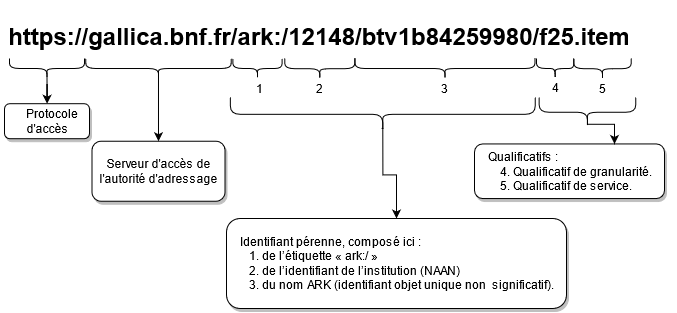
\includegraphics[width=1\linewidth]{images/schema-ark.png}
    \caption{Permalien disposant d'un identifiant \acrshort{ark},  Chloé Pochon, 2021.}
    \label{fig:ark}
\end{figure}

Vu le volume de données, l'étape de formatage semble considérable. En réalité, le travail effectué se concentre principalement sur le volume d'informations historiques car le volume des identifiants est créé automatiquement. Les identifiants sont plus que nécessaires car ils servent à retrouver et à distinguer les éléments de façon unique et sans ambiguïté. 

\subsection{Des données pour le Web}\label{sous-section:web}
Bien que le projet n'affiche pas la volonté de s'intégrer aux enjeux du Web sémantique, qui vise à rendre les données Web plus compréhensibles pour les machines à l'aide de standards et technologies pour décrire les relations entre les données, il intègre divers formats interopérables spécifiques au Web.

\textbf{\acrshort{iiif}} (\textit{International Image Interoperability Framework}) est un protocole d'échange destiné à standardiser la gestion des images numériques, allant de leur hébergement à leur visualisation\footcite{ROBINEAUComprendre2016}. \acrshort{iiif} facilite l'accès et la manipulation des images en utilisant un cadre commun d'interopérabilité, ce qui réduit les coûts de stockage et favorise une approche écologique des données. Les images, qu'elles soient de documents physiques alors numérisés ou des fichiers nativement numériques, sont accessibles directement depuis leur serveur d'origine, sans nécessiter de ré-hébergement ou de stockage local, même lorsqu'il s'agit de fichiers en très haute définition. Grâce aux \acrshort{api} \acrshort{iiif}, les institutions patrimoniales peuvent partager leurs images de manière standardisée\footcite{INHAbibliotheques2019} car \acrshort{iiif} définit des \acrshort{url} normées pour accéder à un fichier image. Les utilisateurs peuvent les manipuler via des requêtes \acrshort{url} (http(s) ://{domaine}/{identifiant}/{zone}/{taille}/{rotation}/{qualité}.{format})\footcite{FAUREstandard2022}, permettant des ajustements comme le cadrage, la rotation et le redimensionnement, tout en préservant les fichiers originaux sur le serveur d'origine. L'ensemble des documents numérisés et sélectionnés pour le projet Richelieu sont dotés d'\acrshort{url} \acrshort{iiif}. Ils seront donc accessibles en \acrshort{iiif} directement depuis l'application. Du point de vue de l'application, cela signifie que les images ne sont pas accessibles via un dossier d'images stockées sur un serveur \acrshort{inha}. Elles sont servies via un catalogue d'\acrshort{url}s aggrégeant des ressources stockées dans plusieurs bibliothèques numériques (\textit{\acrshort{iiif} Stores})\footcite{INHAbibliotheques2019}.

Le \textbf{\acrshort{json}} (\textit{JavaScript Object Notation}) est l'autre format léger utilisé en grande partie sur le projet. Facilement compréhensible pour un œil humain novice, il est utilisé pour structurer et échanger des données entre serveurs et clients, en particulier dans les applications Web. Sa structure simple repose sur des paires clé-valeur où les clés sont des chaînes de caractères et les valeurs peuvent être des chaînes, des nombres, des tableaux, des objets ou des booléens. Le \acrshort{geojson} est une norme de description de données spatiales au format \acrshort{json}. Il utilise les mêmes paires \enquote{clé~:~valeur} mais introduit des types géographiques tels que Point, Polygon, et MultiPolygon (pour ceux qui concernent le projet) pour encadrer les informations géographiques, avec des coordonnées exprimées en latitude et longitude selon le système WGS84, assurant une compatibilité étendue avec divers systèmes de cartographie. \acrshort{json} et \acrshort{geojson}, grâce à leur compatibilité avec de nombreux langages de programmation et leur adoption généralisée dans les \acrshort{api}, sont essentiels pour l’interopérabilité et l’échange efficace de données sur le Web.

Pour conclure, des formats de données interopérables pour le Web sont utilisés, conçus pour être compatibles et fonctionnels sur diverses plateformes, systèmes et applications sans nécessiter de conversion ou d’adaptation particulière. Ces formats simplifient l'échange, l'intégration et l'exploitation des données entre différents systèmes, ce qui est essentiel dans un environnement Web où les données proviennent de sources variées et sont utilisées par diverses applications. Ces types de données évitent ainsi le problème de l'isolement (\enquote{effet silos}) souvent associé aux bases de données traditionnelles. Cependant, un point important convient d'être relevé : le projet Richelieu ne s'intègre pas complètement au Web des données (\textit{Linked data}) dans la mesure où seule une petite proportion de ses données respectent les normes et standards du \acrshort{w3c}. 

\subsection{Choix sur le \acrshort{sgbdr} : PostgreSQL et le modèle client-serveur}
A présent, les données sont prêtes pour être stockées dans une base et être gérées par un système de gestion.
\subsubsection{Définition et critères de choix d'un \acrshort{sgbdr}}
Un système de gestion de base de données relationnelles (\acrshort{sgbdr}) est un logiciel conçu pour créer, gérer et manipuler des bases de données structurées en tables interconnectées par des relations\footcite{HAINAUTBases2022}. Un \acrshort{sgbdr} n’est pas une base de données en soit, mais un outil pour la gérer. Cet outil n'est pas constamment accompagné d'une interface graphique. Il existe aussi des systèmes de gestion de bases de données (\acrshort{sgbd}) qui ne sont pas relationnels. Le \acrshort{sgbdr} garantit l’intégrité et la cohérence des données tout en permettant des opérations flexibles et complexes de requêtage. Pour ce faire, il existe des langages de requête standards tel que le \acrshort{sql} (\textit{Structured Query Language}). Le \acrshort{sql} est un langage informatique qui permet de communiquer avec les bases de données. Il est ainsi utilisé pour effectuer des opérations \acrshort{crud} (\textit{Create, Read, Update, Delete}), soit l'ajout, la lecture, la mise à jour, la suppression. Il permet ainsi la récupération de données via des requêtes \textit{SELECT}. Le choix d'un \acrshort{sgbdr} dépend des besoins spécifiques du projet, comme le type de données, le volume à gérer, la sécurité requise et les performances attendues\footcite{HAINAUTBases2022}. Dans le projet Richelieu, PostgreSQL a été retenu pour sa compatibilité avec divers types de données, dont les données géospatiales grâce à l'extension \acrshort{postgis}, sa performance avec de grands volumes de données, et sa conformité aux standards \acrshort{sql}. Open source et gratuit, il est compatible avec plusieurs systèmes d'exploitation (Mac, Windows, Linux) et bénéficie du soutien d'une communauté active, ce qui en fait une solution robuste et évolutive pour le projet. 

\subsubsection{Le modèle client-serveur : un peu de vocabulaire}
PostgreSQL est un système de gestion de base de données relationnelle qui utilise une architecture client-serveur. Cela signifie que la base de données est hébergée sur un serveur, accessible depuis plusieurs applications clientes via le protocole \acrshort{http}. Même dans une installation locale, la base de données est gérée sur un serveur, et les programmes qui y accèdent sont considérés comme des clients.

Parmi les outils clients, psql est une interface en ligne de commande installée par défaut avec PostgreSQL, permettant de se connecter à une base de données pour effectuer des tâches administratives (comme la gestion des comptes utilisateurs et des bases de données) et d'exécuter des requêtes \acrshort{sql} (afin de voir le contenu de la base). Mais il est aussi possible d'utiliser un autre outil client pour interagir avec la base telles que les interfaces graphiques. pgAdmin est l'interface graphique choisie par le projet, ce logiciel client est donc séparé et offre une interaction visuelle avec PostgreSQL. L'administration et la gestion des bases de données sont facilités par un ensemble de plugins telles que des visualisations de données analysant le contenu de la base. Enfin, postgres désigne à la fois la partie serveur de PostgreSQL, qui gère les fichiers de la base de données et les connexions clients, et le compte administrateur (une donnée administrative) par défaut créé lors de l'installation de PostgreSQL. 

Ces distinctions sont importantes à retenir : \acrshort{sql} est un langage, tandis que psql est un outil client au même titre que pgAdmin, dont le premier est utilisé par les seconds ; ainsi le modèle client-serveur désigne un mode de communication entre deux programmes : entre celui qui envoie les requêtes (le client) et celui qui y répond (le serveur). 

Cette communication sur le réseau Internet est effectuée via des protocoles standards comme \acrshort{http} et \acrshort{https}. Les requêtes et les réponses sont encapsulées dans ce protocole. Cela permet notamment l'échange d'information entre deux systèmes distants. 

\subsection{Le stockage physique à l'\acrshort{inha}}
L'\acrshort{inha} dispose de ses propres serveurs pour l'hébergement de données et de solutions logicielles. Ainsi, la base de données et l'application du projet Richelieu sont centralisées sur un serveur interne à l'institution, ce qui permet aux équipes d'accéder en continu à leurs données, même en l'absence de connexion Internet. Cette centralisation facilite les mises à jour et les opérations de maintenance, tout en assurant une sécurité accrue, l'institut conservant un contrôle total sur ses données sans recourir à des services \textit{Cloud} externes. L'infrastructure informatique de l'\acrshort{inha} est répartie sur deux bâtiments, la galerie Colbert et le quadrilatère Richelieu, séparés par la rue Vivienne. Cette répartition, bien que redondante en apparence, renforce la résilience du système et permet une distribution efficace des ressources et des services essentiels, réduisant ainsi les risques de panne. En cas de développement futur du projet, cette configuration facilite la scalabilité du modèle de données, permettant l'ajout de serveurs supplémentaires pour gérer un volume accru de données. Cette situation d'hébergement devra être prise en compte si le projet est repris par une autre institution, car cela impliquerait également une migration des données sur un autre serveur. 

\subsubsection{Conclusion}
Cette section a permis de mettre en lumière le processus minutieux qui a permis de passer du code brut au stockage des données tout en respectant les exigeances de l'INHA. Ce processus, bien que long et itératif, a affiné les méthodes de traitement des données et permet à l'ingénieur de crééer sa propre boîte à outils pour des traitements à venir. Constituée de plusieurs scripts, cette boîte à outils s'est avérée indispensable pour nettoyer, organiser et structurer les données de manière cohérente. Finalement, ce travail a été guidé par un objectif clair : rendre accessible et exposer les données sur une plateforme Web. 

%%%%%%%%%%%%%%%%%%%%%%%%%%%%%%%%%%%%%
% SECTION %%%%%%%%%%%%%%%%%%%%%%%%%%%
\section{Une application Web pour exposer la donnée}\label{section:web}
Bien que la base de données, structurée en tables, puisse être considérée comme une première forme de présentation des données, elle reste accessible uniquement à un public initié aux interfaces en ligne de commandes. Or le projet vise une communauté scientifique élargie ainsi que le grand public, qui seraient désavantagés sans une interface supplémentaire pour explorer ces données. Il est donc essentiel de créer une présentation des données organisée en plusieurs modules correspondant aux principaux axes du projet : l'iconographie, l'espace, le temps, et les réseaux. Ces modules, qui prennent la forme d'une interface graphique (comme un catalogue iconographique, une cartographie, ou des tableaux), permettent la consultation, la manipulation, et l'analyse des données. 
Ils sont intégrés à une application, qui dans ce contexte, est un programme hebergé sur les serveurs distants de l'\acrshort{inha} et accessible via un navigateur Web. N'importe quel appareil connecté au réseau Internet peut accéder à l'application via l'\acrshort{url} du projet, sans installation spécifique. Bien que l'application puisse ressembler à un site Web, elle offre un niveau de fonctionnalité et de complexité plus élevé. En effet, un site Web se concentre généralement sur la diffusion d'informations à travers des pages statiques, tandis qu'une application, notamment dans le cadre du projet Richelieu, permet des interactions dynamiques et interactives et une gestion de données plus avancée. En outre, son architecture offre des avantages significatifs pour le développement technique, en facilitant l'évolution et l'adaptation du projet. 

\subsection{Architecture de l'application : choix des \textit{Frameworks}}
L'architecture de l'application peut être envisagée comme la colonne vertébrale du projet final, où chaque vertèbre qui la compose représente un dossier de fichiers interconnectés. L'application est divisée en deux grandes parties distinctes : le \textit{front-end} et le \textit{back-end}. Chacune de ces parties est généralement développée par un ingénieur spécialisé, bien que certains ingénieurs maîtrisent les deux aspects et se chargent du développement \textit{fullstack}, comme c'est le cas pour le projet Richelieu. Ces deux parties ont pour but de connecter la base de données à l'utilisateur via une interface graphique. Leur rôle sont distincts mais complémentaires. Pour développer ces parties, il existe de multiples cadres de travail, appelés \textit{Frameworks} qui sont en réalité des outils qui accélèrent le développement, organisent et structurent le code, améliorent la sécurité et surtout facilitent la gestion d'un projet informatique. 

\subsubsection{Pour le \textit{back-end}: Flask et SQLAlchemy}
L'objectif du \textit{back-end} est la gestion et la manipulation des données stockées dans la base avec laquelle il intéragit pour lire, écrire, envoyer, mettre à jour et supprimer des information. Il implémente une logique métier qui sont un ensemble de règles et de processus qui définissent le comportement de l'application comme la validation des données, la typologie des données, certains calculs éventuels. Il met aussi en œuvre certains mécanismes d'authentifications que nous avons cités plus haut. En essence, il constitue la partie cachée de l'application, semblable aux coulisses d'un spectacle où se préparent les acteurs, les costumes et les accessoires. Les langages de programmation utilisés pour cette partie sont variés, parmi eux se trouvent Java, \acrshort{php}, Node.js, voire Ruby et particulièrement Python -- le langage de haut niveau utilisé pour le projet Richelieu. Pour simplifier le développement de l'application, Flask, un micro-framework web pour Python, a été utilisé. Flask est léger, flexible et robuste, ce qui permet de créer des applications web rapidement et efficacement. Sa facilité d'apprentissage le rend accessible même aux développeurs débutants. Bien qu'il offre de nombreuses fonctionnalités préconçues, telles que le routage des \acrshort{url} et la gestion des requêtes \acrshort{http}, Flask n'impose pas de structure rigide, permettant ainsi l'ajout d'extensions telles que la gestion des formulaires et l'authentification. Flask permet également d'intégrer SQLAlchemy, une bibliothèque Python qui facilite le mappage objet-relationnel (\acrshort{orm} : \textit{Object-Relationnal Mapping}). Cela signifie qu'il simplifie la modélisation physique des données de la base en permettant de représenter chaque table sous forme de classes Python, plutôt que de requêtes SQL. Ainsi, les données sont manipulées via des objets Python, adoptant une approche de programmation orientée objet pour interagir directement avec PostgreSQL. Ces objets sont codés dans le dossier \acrshort{orm} (voir la figure \ref{fig:app}.

Cette abstraction des opérations relationnelles complexes est facilitée par une \acrshort{api} (\textit{Application Programming Interface}). Il s'agit d'une interface qui spécifie la manière dont différentes parties d'un système ou d'une application peuvent interagir. 

Ces interactions sont rendues possibles grâce à des \textit{endpoints} (portes d'entrée), c'est-à-dire des \acrshort{url}s spécifiques servant de points d'entrée pour l'échange d'informations. Fonctionnant sur des requêtes \acrshort{http}, cette \acrshort{api} est interne à l'application et est accessible uniquement par les développeurs. Par ailleurs, une autre \acrshort{api}, publique et conforme au protocole REST, est également prévue pour le développement du projet, et nous aborderons ce sujet plus en détail ultérieurement. Le dossier \texttt{routes} sauvegarde ainsi les scripts python codant l'\acrshort{api} soient les différentes portes d'accès des informations envoyées au \textit{front-end}.


\subsubsection{Pour le \textit{front-end}: Vue.js}
L'objectif du \textit{front-end} est de concevoir l'interface utilisateur (UI) et l'expérience utilisateur (UX) afin de rendre le contenu accessible et agréable pour les utilisateurs. Pour prolonger la métaphore filée, le \textit{front-end} est l'espace visible où se déroule le spectacle auquel les spectateurs assistent. Il est donc responsable de l'affichage des données fournies par \textit{back-end} sur les pages de contenu, les boutons, les graphiques, les cartes, et les descriptions d'œuvres en s'assurant que la navigation entre ces éléments soit fluide, agréable, dynamique, et sans erreurs. Pour structurer et présenter ces informations, trois langages principaux sont utilisés : \acrshort{html} (\textit{HyperText Markup Language}), qui définit la structure des pages web ; \acrshort{css} (\textit{Cascading Style Sheets}), qui gère le style et l'apparence visuelle ; et JavaScript qui rend l'application interactive et dynamique. Pour simplifier et optimiser le développement de cette partie, nous utilisons le \textit{Framework} Vue.js. Celui-ci repose sur une architecture basée sur des composants, chaque composant étant une unité autonome de l'interface utilisateur qui regroupe le code \acrshort{html}, \acrshort{css} et JavaScript. Cette approche permet la réutilisation et l'imbrication des composants, favorisant une structuration modulaire de l'application. En cas de bug dans un composant, celui-ci n'affecte pas les autres, car chaque composant fonctionne indépendamment. Vue.js offre également des fonctionnalités communes à tous les \textit{Framwork} qui visent à permettre une meilleure interaction entre les données, une meilleure structuration en \acrshort{html} et une meilleure manipulation en JavaScript. 

Sa capacité à s'intégrer de manière progressive permet d'ajouter des éléments au fur et à mesure. La scalabilité facilité son intégration dans des projets existants sans nécessiter une réécriture complète. De plus, Vue.js est bien documenté, ce qui facilite son apprentissage et son utilisation pour les développeurs de tous niveaux. Enfin, Vue.js est compatible avec tous les navigateurs Web, assurant une interaction fluide avec les différentes plateformes. 

Ainsi, telle est la structuration de l'architecture de l'application du projet Richelieu, comme le synthétise le schéma arborescent\footnote{Pour plus de détails, se référer au schéma complet en annexe \ref{fig:archi-détaillée}.}

\begin{figure}
    \centering
    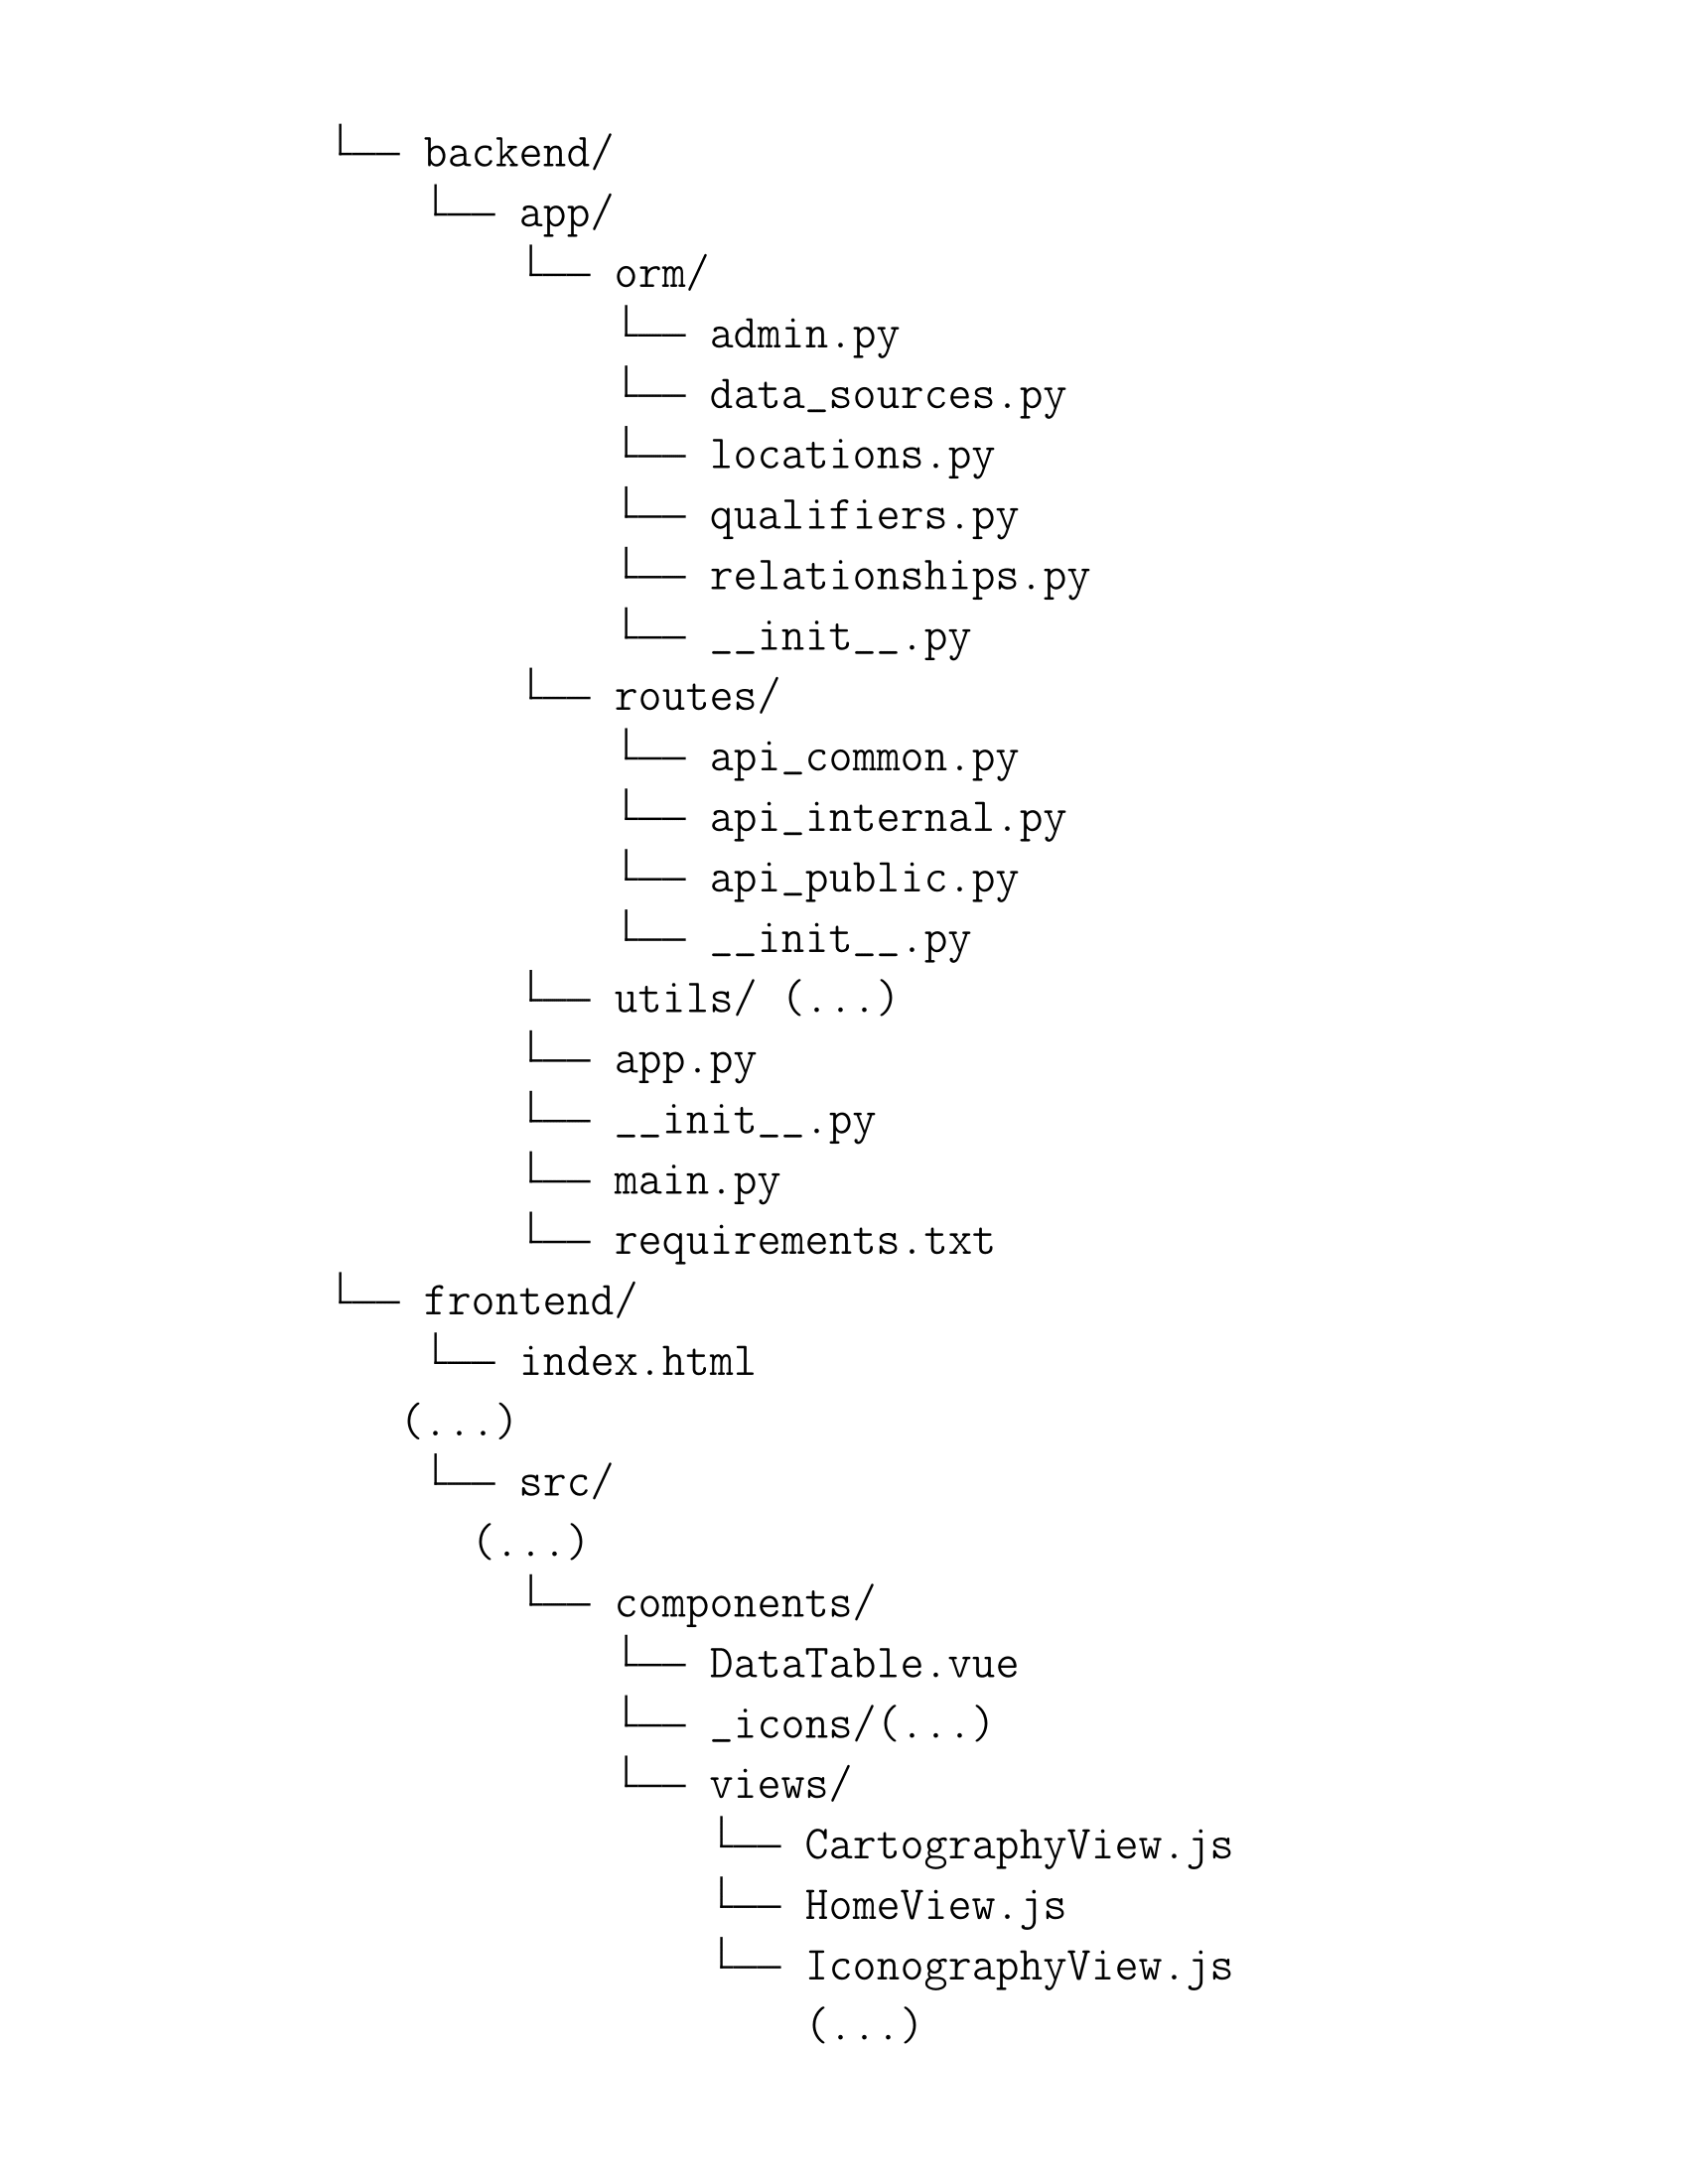
\includegraphics[width=0.5\linewidth]{images/architecture_appli_simplE.png}
    \caption{Arborescence simplifiée de l'application, \mhd.}
    \label{fig:app}
\end{figure}

\subsubsection{Quelques contraintes de développement}
Bien que le cadre de travail pour le développement de l'application intègre des outils puissants, leur prise en main peut être complexe pour un débutant. Chacun de ces outils peut sembler facile à utiliser individuellement, mais les combiner pour créer une architecture solide nécessite un certain temps d'adaptation. Par exemple, Vue.js offre de nombreux atouts de développement que nous avons présentés mais pour pouvoir l'utiliser, cela présuppose une solide maîtrise des langages du \textit{front-end} (\acrshort{html}, \acrshort{css} et JavaScript) -- ce qui n'est pas nécessairement le cas pour un stagiaire. Pourtant une compréhension approfondie de leur fonctionnement est indispensable pour exploiter pleinement les fonctionnalités de Vue.js. C'est pourquoi, après plusieurs tentatives et nombreux blocages, il a été décidé de développer la cartographie Web en dehors du \textit{Framework} Vue.js. Cette décision n'a pas d'impacts importants sur le développement général de l'application. 

\subsection{Les différents niveaux de communication client-serveur.}
\begin{figure}
    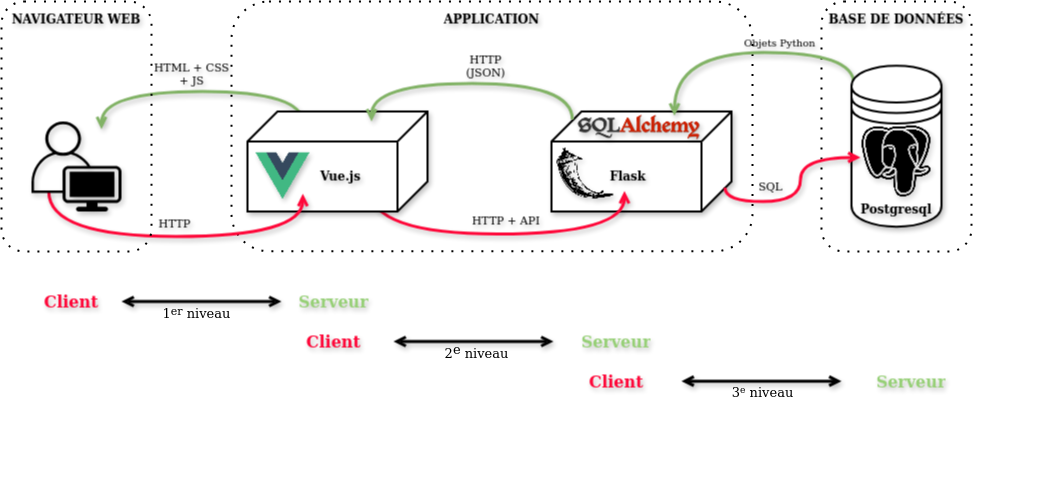
\includegraphics[width=1\linewidth]{images/Niveaux_communication_application.png}
    \caption{La communication client-serveur de l'application, \mhd.}
    \label{fig:enter-label}
\end{figure}
Pour transmettre l'information depuis la base de données jusqu'au navigateur Web via l'application, différents niveaux de communication client-serveur sont mis en place. Le premier niveau comprend le navigateur web, utilisé par l'utilisateur final, interagit avec l'application web construite avec Vue.js. Dans ce contexte, le navigateur agit en tant que client, envoyant des requêtes utilisateur à Vue.js, qui fonctionne comme un serveur pour ces interactions. Le deuxième niveau d'interaction, depuis Vue.js, après avoir traité l'interaction utilisateur, devient à son tour le client en envoyant des requêtes \acrshort{http} au back-end géré par Flask. Flask agit ici comme le serveur, répondant aux requêtes en fournissant les données nécessaires pour mettre à jour l'interface utilisateur. Le troisième, Flask, après avoir reçu la requête de Vue.js, se transforme en client en interrogeant la base de données PostgreSQL pour obtenir les informations demandées. SQLAlchemy joue un rôle intermédiaire ici, facilitant la communication entre Flask et PostgreSQL en convertissant les objets Python en requêtes SQL. PostgreSQL, en tant que serveur, répond à ces requêtes \acrshort{sql} en renvoyant les données nécessaires. À chaque étape, les rôles de client et serveur changent, illustrant la complexité et la modularité de l'architecture. Cette structure permet de découpler les différentes responsabilités de l'application, facilitant ainsi sa maintenance, son évolution et sa scalabilité. 
Pour un développement de l'application en local, l'architecture reste la même. 

%%%%%%%%%%%%%%%%%%%%%%%%%%%%%%%%%%%%%
\subsubsection{Conclusion du chapitre} 
En conclusion, les états successifs de la donnée du projet Richelieu illustrent la complexité croissante des objets numériques dans un environnement de plus en plus interconnecté. La structuration des données pour la cartographie Web démontre que la simple numérisation d’un corpus, qu’il soit iconographique ou cartographique, dépasse largement la production d’une image numérique. Il s'agit de la création d’un objet numérique sophistiqué, enrichi de métadonnées descriptives et structurelles, qui permet de révéler la profondeur et la richesse de l’information contenue dans ces documents. Cela amène à s'interroger sur le passage du Web de documents, où les ressources sont principalement statiques, au Web de données, où l'information est dynamique, interrogeable et exploitable, créant ainsi de nouvelles perspectives pour la recherche et la diffusion du savoir.

%%%%%%%%%%%%%%%%%%%%%%%%%%%%%%%%%%%%%
\subsubsection{Conclusion de la première partie} 
La base de données du projet Richelieu, bien que peu volumineuse avec ses 100~000 entrées, reflète avec précision les multiples facettes du quartier et incarne l'essence même de son nom : Richelieu, un lieu riche en histoire et en significations. Ce lieu occupe une position centrale dans la conception et l'orientation du projet. Le système développé pour soutenir cette ambition est à la fois robuste et d'une complexité technique relative, nécessitant un véritable investissement en temps pour être analysé, compris et maîtrisé par l'ingénieure novice. Après de longues étapes de saisie, d'encodage et de stockage des données, le projet s’est doté de l’infrastructure technique nécessaire pour réaliser ses ambitions scientifiques et mettre en lumière la richesse des informations qu’il contient.

%%%%%%%%%%%%%% PART 2 %%%%%%%%%%%%%%%%%%%%%%%%%%%%%%%%%%%
%%%%%%%%%%%%%%%%%%%%%%%%%%%%%%%%%%%%%%%%%%%%%%%%%%%%%%%%%
\part[Réalisation technique : la carte, un outil d'exploration des données]{Réalisation technique : \\la carte, un outil d'exploration des données}
Cette deuxième partie se concentre sur l'objet de mon stage qui est aussi le cœur du mémoire : la cartographie Web. Elle met en lumière les différentes réflexions préalables à la réalisation technique de la carte, ainsi que le développement informatique concret de celle-ci. Plusieurs questions essentielles sont abordées : Quelle typologie de visualisation cartographique est adaptée au projet ? Quelles fonctionnalités sont attendues, espérées ou réalisables pour cette carte ? Peut-elle intégrer les différentes dimensions du projet, à savoir l'iconographie, le temps, l'espace et le réseau ? Si oui, de quelle manière ? Si non, ces limites sont-elles liées à la structure des données ? Quelles sont les propositions graphiques pour la carte ? Quels avantages la carte offre-t-elle en tant qu'outil d'exploration des données Web ? À quel public s'adresse-t-elle ? Comment garantir l'intégrité des données affichées par la carte ? Quelles techniques d'ingénierie permettent d'éviter l'effet « boîte noire » ? Enfin, la carte est-elle à la hauteur des ambitions scientifiques pour retranscrire les hypothèses de recherche ?

%%%%%%%%%%%%%% CHAPT 3 %%%%%%%%%%%%%%%%%%%%%%%%%%%%%%%%%%
\chapter{Les objectifs de la cartographie Web}
\chaptermark{Définir des objectifs}
% PARTIE 2 - TECHNIQUE %%%%%%%%%%%
% CHAPITRE 3 %%%%%%%%%%%%%%%%%%%%%
%%%%%%%%%%%%%%%%%%%%%%%%%%%%%%%%%%
Pour développer une carte Web, il ne suffit pas d'avoir des données structurées dans une base de données, il est également nécessaire de concevoir leur agencement et leur visualisation\footcite{LAGNELManuel2021, ANDRYChapitre2022, CEJUDObreve2022}. Ce troisième chapitre introduit une nouvelle étape de conception de la carte qui consiste à définir des objectifs de développement spécifiques à la cartographie Web. Dans un premier temps, ces objectifs sont établis en comparant divers éléments de cartes Web issues de projets de recherche. Après cette présentation de l'état de l'art, il s'agit de hiérarchiser les priorités de développement à l'aide de plusieurs méthodes. Enfin, une analyse du contenu de la base de données est intégrée à ce processus : il apparaît en effet primordial de bien comprendre le contenu avant de l'intégrer dans l'application pour le développement de la carte. Cette analyse quantitative permettra d'anticiper les possibles biais de représentation qui pourraient survenir lors de la visualisation.

%%%%%%%%%%%%%%%%%%%%%%%%%%%%%%%%%%%%%
% SECTION %%%%%%%%%%%%%%%%%%%%%%%%%%%
\section{État de l'art de la visualisation cartographique des données sur le Web}\label{section:choix-carto}
Cette première section offre un aperçu non exhaustif de l'état de l'art des visualisations cartographiques des données sur le Web. En couvrant à la fois la réflexion théorique et la mise en œuvre technique, seront listés et comparés des éléments cartographiques de projets de recherche, en particulier en histoire de l'art. Ce tour d'horizon sert à donner quelques repères et points de référence pour définir au mieux les fonctionnalités à privilégier et celles à mettre de côté pour la visualisation de données géohistoriques du projet Richelieu.

\subsection{En théorie : l'image est une écriture}
Rappelons-le, la visualisation est une \enquote{présentation visuelle sur un écran, sous \textit{forme d'image} alphanumérique ou graphique, d'un ensemble d'informations traitées par des moyens informatiques} (Larousse). Pourquoi le projet Richelieu favorise-t-il l’utilisation de l’image plutôt que de celle de l'écriture pour explorer et étudier le quartier~?  Dans les sciences humaines et sociales, l'écriture demeure la forme conventionnelle de l'expression scientifique. En histoire de l'art, cette tradition est d'autant plus marquée que l'écriture sert à décrire et à interpréter les œuvres. Dans ce cas, l'image est ainsi secondaire à l'écriture. Toutefois, il est reconnu que les enluminures, gravures, peintures, photographies et autres représentations graphiques sur une surface plane servent tout autant à exprimer un propos\footcite{GRANDJEANIntroduction2015}. L'image est un moyen d'expression visuelle. La visualisation des données s'introduit dans cette chronologie des traditions narratives. L’écriture est également une expression mais par son système de signes conventionnels, il s'agit d'un moyen écrit. Les deux fournissent un effort d’abstraction pour rendre le sensible, le réel et le matériel visible. Toutefois, l’image permet d'atteindre un niveau d'abstraction que l'écriture ne peut pas toujours atteindre, offrant une échelle de représentation différente et souvent plus immédiate pour visualiser le réel\footcite{CHRISTINLecriture2020}. Il est par exemple plus simple de représenter le globe terrestre par une image que par un texte. 

Même si un proverbe dit qu'\enquote{une image vaut mieux que mille mots}\footnote{Ce proverbe est attribué à Confucius.} elle ne peut se réduire à elle-même dans le domaine scientifique. Cela ne signifie pas pour autant qu'elle soit nécessairement accompagnée d'un texte écrit sinon de connaître la démarche dans laquelle la visualisation a été réalisée. Cette idée est principalement développée par l'historien contemporanéiste et spécialiste des humanités numériques, Martin Grandjean, qui estime qu'\enquote{il faut distinguer les visualisations qui \textit{découlent} d’un savoir scientifique et les visualisations qui \textit{créent} un savoir scientifique}.\footcite{GRANDJEANIntroduction2015} En d'autres termes, il définit deux objectifs de visualisation : celle à des fins de \textit{démonstration} d'un savoir déjà établi et celle qui sert à la \textit{recherche} pour constituer un nouveau savoir. Cette distinction fondamentale clarifie l'objectif de la démarche visuelle. En effet, dans le premier cas, les visualisations sont utiles pour rendre un savoir accessible et compréhensible, à des fins pédagogiques par exemple. Tandis que le second cas a pour but d'explorer des données complexes révélant des questions nouvelles voire des perspectives de recherches inattendues. Il affirme par ailleurs que ce dernier cas n'est pas destiné à être publié. 
\begin{figure}[ht!]
    \centering
    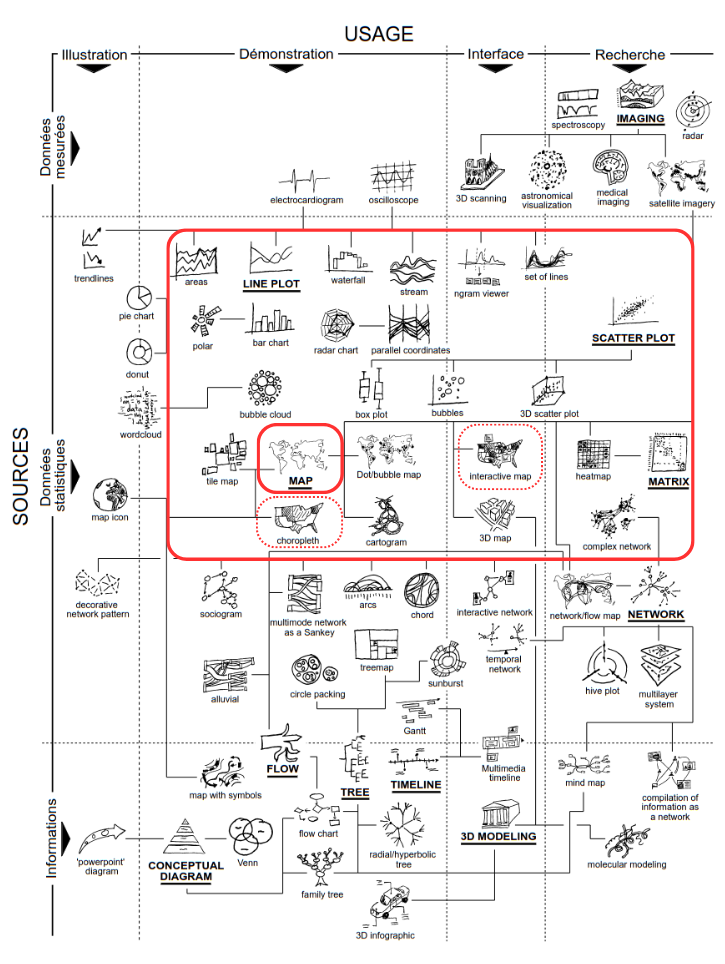
\includegraphics[width=1\linewidth]{images/typologie_dataviz.png}
    \caption{Typologie de la visualisation de données selon deux axes : le type de sources
utilisées (vertical) et le type d’usage (horizontal), Grandjean, 2022.}
    \label{fig:typologie_dataviz}
\end{figure} 

Qu'en est-il du projet Richelieu ? La visualisation des données telle qu'elle a été définie par le projet correspond aux deux cas. Certains axes de recherche sont confirmés et rédigés au sein d'articles scientifiques. Dans ce cas, la carte est une démonstration de ce qui est déjà prouvé, dit et connu. Mais la carte est aussi attendue comme outil de recherche à travers laquelle des hypothèses sauraient se formuler. Surtout, la carte a pour but d'être publiée et à destination d'un large public, aussi bien expert que novice. Ce caractère ambivalent de la carte créé une ambiguïté qui est également établie par l'auteur mais au sein d'une autre de ses publications\footcite{GRANDJEANvisualisation2022} dans laquelle il dresse une classification des typologies de visualisations de données. Parmi ce large panorama, la carte offre un caractère ambivalent oscillant entre visualisation de \enquote{démonstration} et de \enquote{recherche}. 

Il existe de nombreuses classifications des typologies de visualisations de données\footnote{Parmi les plus connues : le \href{https://github.com/Financial-Times/chart-doctor/blob/main/visual-vocabulary/poster.png}{Visual Vocabulary} du Financial Time, les catalogues \href{https://datavizcatalogue.com/FR/}{Data Visualization Catalog}, le \href{https://datavizproject.com/}{Data Viz Project} et le \href{https://flowingdata.com/chart-types/}{Flowingdata}. Cliquer sur le nom des typologies pour accéder aux sites Web.}  mais celle que Grandjean propose est intéressante à plusieurs titres (\ref{fig:typologie_dataviz}). Tout d'abord, sa classification est une aide réelle avant la mise en production d'une visualisation. En fonction des types de sources utilisées et des types d'usage définis, une forme de visualisation peut se distinguer. 

Pour le projet Richelieu, les sources sont des données extraites, en opposition aux informations généralistes, ce qui réduit considérablement le type de visualisations. Un \acrshort{uuid} n'est pas comparable au schéma numérique de la \acrshort{bnf} par exemple. Il ne s'agit pas en effet d'une infographie qui repose sur la compilation d'informations impliquant une approche plus \enquote{manuelle} mais bien d'une visualisation pour laquelle les données sont \enquote{automatiquement} captées par un outil informatique dont le résultat est parfois plus difficilement contrôlable. Ensuite, nous savons que la visualisation du projet a pour objectif d'être utilisée comme une interface, et, selon le graphe, elle est à l'intersection de la démonstration et de la recherche. Enfin, parmi les grandes familles de typologies de visualisations, telles que le nuage de points, le réseau ou le graphique en ligne ou en barre, la carte s'impose pour le projet Richelieu - notamment en raison du caractère spatial des données. Selon la définition de Grandjean, la carte se décline alors  en de nombreuses autres typologies secondaires, parmi lesquelles deux se démarquent : la carte choroplèthe et la carte interactive. La première proposition organise la donnée par zone, nos lieux symbolisés par les polygones, qui respecte la réalité géographique et est structurée en variable de données. Cela permet ainsi de visualiser les variations de données d'une zone à une autre, souvent signifiées par la couleur. La seconde carte est plus évidente puisque c'est une interface qui permet d'accéder aux données et d'interagir avec elles, et que le projet utilise les langages du Web interactif, dont le JavaScript dans Vue.js. La carte du projet Richelieu serait donc une association de ces deux typologies. Même si l'auteur rappelle aux développeurs que sa classification n'est pas exhaustive et encore moins impérative, elle présente quelques pistes de réflexion non négligeables pour catégoriser les visualisations. 

Ainsi la carte, en tant que visualisation, est accompagnée d'une riche historiographie. Parmi elle, Jacques Bertin théorise, à partir de la seconde moitié du XX\ieme siècle, la science de la représentation graphique des données dans un traité fondateur : \textit{Sémiologie graphique. Les diagrammes, les réseaux, les cartes} publié en 1967. Il instaure l'idée que la visualisation doit répondre au critère d'\textit{efficacité}\footcite{BERTINSemiologie1967} (p.139) : 
\begin{displayquote}\enquote{Il importe donc de définir un critère précis, mesurable, à partir duquel on puisse classer les constructions, définir incontestablement la meilleure et expliquer, s’il y a lieu, pourquoi certains lecteurs préfèrent une construction et certains une autre. Nous appellerons ce critère l'\textit{efficacité}. [...] si pour obtenir une réponse correcte et complète à une question donnée, et, toutes choses égales, une construction requiert un temps d’observation plus court qu’une autre construction, on dira qu’elle est plus efficace pour cette question.}
\end{displayquote}

Selon lui, il existe une multitude de représentations graphiques pour une information mais certaines sont plus efficaces car le \enquote{coût} mental de compréhension est moindre. Les formes sont perçues dans l'instant. Cette théorie de la représentation graphique s'accompagne également d'une large grammaire de signes, formes et couleurs inspirant ainsi de nombreuses cartes. Mais cette conception présuppose que la compréhension est la même pour tous les être humains, or aucun système ne saurait être universel. Bien que la théorie bertinienne pose les fondements de la cartographie en tant que discipline pour la distinguer de la géographie dont elle est parente\footcite{CFCHistoire2024}, elle est réductrice et ses idées installées sont renversées par une riche historiographie contemporaine. A l'inverse de l'\enquote{efficacité}, Anthony Masure propose une \enquote{méthodologie du doute où le dessin échappe au dessein}.\footcite{MASUREDesign2017} Certains prônent une cartographie radicale\footcite{ZWERCartographie2022} , d'autres -- parmi lesquels Joahanna Drucker en représente la figure de proue  -- appellent à l'interprétation modélisante (\textit{modelling interpretation})\footcite{DRUCKERVisualisation2020} des visualisations. Un historien de l'art de l'XIX\ieme~,  Victor Claas, résume son propos\footcite{CLAASJohanna2021}:
\begin{displayquote}
\enquote{ Rendant manifeste les dangers et les points aveugles d’une relation entre les données et leur visualisation envisagée de manière trop littérale, Drucker propose une approche plus aventureuse de la pensée graphique. Celle-ci place la production d’images au service de la formulation des savoirs et de la pensée critique.}
\end{displayquote}
Constituées sur les fondements des \textit{cultural studies}, de la pensée décoloniale\footcite{HANCOCKDecoloniser2008} ainsi que de la théorie \textit{queer}, les réflexions de Drucker expriment l'idée que la toute-puissante mise en données ne saurait être exclue de son contexte de production car la donnée, plutôt à considérer comme \textit{capta} n'est jamais neutre ou désaffectée sinon saisie et capturée. 

C'est au sein de ce terrain historiographique que les cartes, que nous avons consultées et dont nous comparons quelques éléments, s'appuient ou renoncent à ces conceptions. 

\subsection{En pratique : un tour d'horizon des cartes Web de projets de recherche}
Afin de poursuivre cette étape conceptuelle de la carte, nous dressons un état de l'art des projets analogues au projet Richelieu. \footnote{Les exemples de cartes sont nombreux dans le domaine de la recherche en \acrshort{shs}, celles que nous avons choisies constituent un échantillon fréquemment cité. En histoire de Paris, on retrouve notamment les cartes \href{https://vergue.com/carto-vergue-paris/}{Vergue} et celle consacrée à la \href{https://fnp.huma-num.fr/aws/app/714c416a-fd4b-11ec-a932-a50d533ee08c/index.html?dummy=1658312704504}{Rafle du Vel'd'Hiv} du CstPTM ;  en histoire de l'art : \href{https://paris-art-market.huma-num.fr/}{le projet Artl@s}, \href{https://datavirgo.huma-num.fr/}{DataVigro}, \href{https://datart.huma-num.fr/}{DatArt}, et le projet \href{https://www.inha.fr/fr/recherche/programmation-scientifique/en-2023-2024/seminaire-regarts-trajectoires-plurielles-les-eleves-de-l-ecole-des-beaux-arts-de-paris-1800-1968.html}{REGarts} prochainement en ligne; enfin les cartes du studio \href{https://forensic-architecture.org/}{Forensic Architecture} sont souvent prises en exemple tout comme celles du projet \href{https://native-land.ca/?lang=fr}{Native Land Digital}. Cliquer sur le nom des sites Web pour y accéder.} Consulter, comparer et annoter cet échantillon permet d'identifier les pratiques existantes et d'évaluer les forces et les faiblesses des cartes. Pour ce faire, seule la structure de la visualisation et ses composants graphiques sont comparés. Un état de l'art plus approfondi, notamment du point de vue technique, aurait été bénéfique pour connaître les choix informatiques et les développements à reproduire. Même si le code de ces cartes\footnote{Par exemple, le code de DataVirgo est disponible à \href{https://github.com/QuentinEmilianoBernet/DataVirgo-interactive-mapping/blob/main/Datavirgo_source_code.js}{cette adresse}, et celui de Forensic Architecture \href{https://github.com/forensic-architecture/timemap}{ici}.} est disponible en ligne, le temps imparti vient freiner cette volonté d'approfondissement. 

\subsubsection{Un structure commune}
Toutes les cartes présentent une page d'accueil sous forme de \textit{pop-up} qui détaille le projet et explique la navigation le cas échéant. Peu de cartes accordent une grande importance à cet \enquote{à propos}, il est généralement mis en arrière-plan tout en restant accessible durant l'exploration de la carte. De par leur nature, chaque carte affiche un fond de carte, qu'il soit historique ou contemporain. Nombreuses sont celles qui proposent un curseur d'opacité pour comparer la carte historique à la carte contemporaine, mais rares sont les cartes Web qui permettent de suivre une évolution historique à travers une succession de fonds de cartes anciennes. De plus, divers éléments enrichissent le cadre de la carte tels qu'une barre de recherche, une frise chronologique, un \textit{slidebar} ou des filtres à cocher. Quand ces éléments sont sélectionnés par l'utilisateur, de nouvelles données sont affichées sur la carte. Dans l'ensemble, les éléments structurants restent relativement similaires d'une carte à l'autre. 

Néanmoins nous remarquons que les éléments constitutifs d'une carte sont absents, partiellement ou totalement. Le titre, le corps de la carte, la légende, l'orientation telle qu'une flèche indiquant le nord, la barre d’échelle, la source sont des éléments du cartouche constituant un support informationnel pour lire et comprendre la carte\footcite{LAMBERTboite2016, LEFEBVREproduction1974}. Sans eux, la carte reste indéfinie, incomplète, inexploitable et sujette à de mauvaises interprétations. Il est intéressant de remarquer que dans le domaine plus restreint de la cartographie, qu'elle soit sur papier ou assistée par ordinateur, ces éléments sont la condition \textit{sine qua non} de toute production de carte\footcite{COSGROVECultural2008}. Pourquoi les cartographies Web s'en dispensent ? La raison est-elle humaine ou technique ? Des éléments de réponses se dessineront quant nous passerons au développement de la carte. 

Ainsi, nous constatons que les principales différences entre les cartes ne viennent pas de ces éléments structurants sinon du design graphique appliqué à ces composants qui transforment fondamentalement chaque carte, au-delà de ses données.

\subsubsection{Un design graphique varié sur le Web}
Comme nous l'avons vu, le design graphique joue un rôle clé dans l'expression et la compréhension des données, en l'occurrence cartographiques. Les signes, symboles et couleurs utilisés sur les cartes font preuve d'une grande diversité de designs. Appliquée au Web, cette diversité se multiplie car d'autres caractéristiques, telles que l'interactivité et la navigation, entrent en jeu. Ces dernières offrent aux utilisateurs une expérience de navigation dynamique, où les éléments graphiques ne se contentent pas de représenter des données, mais permettent également d'explorer et d'interagir avec elles. Par exemple, un symbole qui indique l'emplacement d'un hôtel sur une carte sera en réalité un bouton qui, au clic, renvoie à d'autres informations connectées via Internet, telles que le siteWeb de l'hôtel. Selon Bénédicte Bucher \footcite{BUCHERcarte2007}, chercheure en géographie et spécialiste du geoWeb\footcite{JOLIVEAUgeoweb2011} : 
\begin{displayquote}
    \enquote{L'interaction doit faciliter l’exploration, soit en affichant des informations supplémentaires sur la ressource correspondant au symbole sélectionné, soit en conduisant directement à la ressource grâce à la navigation hypertexte.}
\end{displayquote}
Cette caractéristique propre à la carte sur le Web induit que l'interaction et la navigation sont aussi à \textit{designer} ce qui donne à toute information annotée sur une carte un très large spectre de possibilités graphiques. Par exemple, une zone d'une carte peut non seulement être colorée mais cette coloration peut être dynamique. En effet, lors du passage de la souris sur celle-ci, son état visuel se modifie, elle est en surbrillance. Au clic, la couleur peut aussi se modifier pour mettre en évidence des informations qui n'étaient pas visibles au premier coup d'œil, rendant l'interaction plus intuitive. Autre exemple, le zoom est également un élément de navigation qui engendre de nombreuses modifications graphiques : il ajoute ou réduit des informations géographiques sur le fond de carte en fonction du niveau de zoom sélectionné. L'affichage des données doit être ajusté, un symbole doit grossir si l'échelle de la carte se réduit et inversement pour que la lecture de la carte reste cohérente et informationnelle. Chaque niveau de zoom induit un design à chaque information annotée sur la carte. Cela multiplie les possibilités d'exploration et de navigation qui sont donc particulièrement larges et avancées pour l'utilisateur et surtout pour le développeur qui doit les conceptualiser.

Par ailleurs, certaines cartes introduisent une interaction inversée où l'utilisateur devient spectateur plutôt qu'acteur, comme avec une \textit{timeline} qui fait évoluer la carte de manière autonome, faisant apparaître ou disparaître les données comme dans un film. Cette dynamique enrichit l'expérience utilisateur en offrant une perspective temporelle sur les données.

Enfin, nous constatons que les phénomènes de cartes sur le Web offrent une gestion relative des langues. Certaines cartes mélangent différentes langues, d'autres offrent des options claires pour choisir la langue de lecture, ce qui facilite la compréhension. Ce manque de clarté nous indique un fait révélateur des cartes sur le Web. 
\\

Si les cartes sur le Web paraissent plus hétérogènes que les cartes analogiques, sur papier, c'est que les technologies pour les réaliser sont multiples\footcite{ARNAUDcarte2023}. Leur prise en main est rapide, elles offrent un large spectre de possibilités pour visualiser graphiquement une information. Mais si un design ne correspond pas à nos attentes, s'il vient biaiser une information telle qu'un point rouge que nous voulons vert, cela demande un peu plus de maîtrise informatique pour dépasser les fonctionnalités structurées par défaut dont tout initié ne sera pas forcément doté.  Ainsi les cartes sur le Web sont faites \enquote{à la carte}, pour reprendre l'expression de Bucher, et c'est pourquoi elles offrent une large sémiologie graphique\footcite{GEOCONFLUENCESSemiologie2024} et font parfois preuve d'un manque de cohérence. À travers ce bref tour d'horizon, ou \textit{benchmark}, il  est ainsi difficile de définir des tendances mais les cartes offrent quelques prescriptions à respecter pour les fonctionnalités de la carte Richelieu - qu'il convient à présent de lister. 

%%%%%%%%%%%%%%%%%%%%%%%%%%%%%%%%%%%%%
% SECTION %%%%%%%%%%%%%%%%%%%%%%%%%%%
\section{Définition des fonctionnalités et des méthodes de développement}
Nous avons établi que la carte constitue une géodatavisualisation pertinente pour le projet Richelieu. Pour concrétiser un projet tel que celui-ci, diverses méthodes et processus peuvent être employés, parmi lesquels les concepts de \textit{Storyboard} et de \textit{Minimum Viable Product} (\acrshort{mvp}) se distinguent.

\subsection{Le \textit{Storyboard} : définir des fonctionnalités}
Le \textit{Storyboard} est traditionnellement associé au monde du cinéma ou de la bande dessinée, pourtant sa fonction scénaristique peut tout aussi bien être appliquée à la conceptualisation d'une carte Web qui, comme nous l'avons dit plus haut, est interactive et dynamique. Il permet de construire l'interface sans le code pour réfléchir aux formes d'interactions avec les données. C'est à partir du \textit{storyboard} que les éléments saillants suivants ont été identifiés. Les éléments principaux à définir en terme de fonctionnalités de la carte sont, pour rappel, le temps, l'espace, l'iconographie ou les réseaux. Ce document n'a pas pour but de réunir les propositions graphiques des éléments mais de présenter des idées quant à leur positionnement et leur interaction. Il cherche aussi à mettre en évidence des lacunes repérées à combler. Surtout, il soulève quelques questions, autant structurelles que techniques. En d'autres termes, c'est un document sur lequel l'équipe du projet s'est appuyé pour accompagner le développement conceptuel de la carte. 

\begin{figure}[h!]
    \centering
    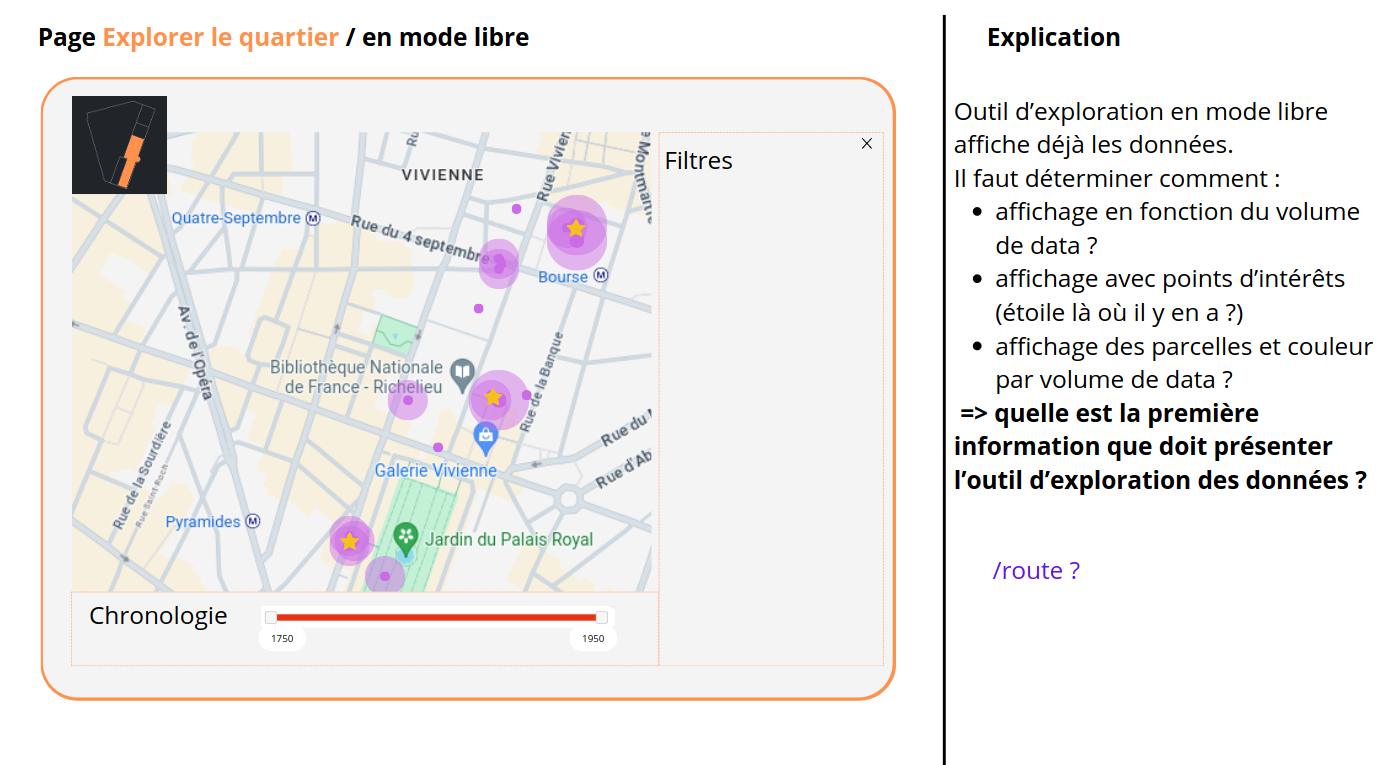
\includegraphics[width=1\linewidth]{images/storyboard-all.png}
    \caption{Storyboard page générale sur la carte}
    \label{fig:story-all}
\end{figure}
\subsubsection{Scénariser l'exploration}
Le premier objet du \textit{Storyboard} a été de scénariser l'arrivée de l'utilisateur sur la carte et de proposer une aide à sa prise en main. Ainsi un onglet \enquote{à propos} est pensé au même titre que ceux que nous avons cités et comparés dans les cartes plus-haut (voir la figure \ref{fig:story-propos}). Une particularité de cette page d'accueil est de proposer une exploration guidée. Si l'utilisateur choisit ce mode d'exploration alors les données affichées sur la carte sont pré-sélectionnées par les chercheurs de l'équipe en fonction d'un sujet pré-défini. Mais l'utilisateur peut également refuser cette proposition guidée pour explorer librement la carte. À partir de ces deux modes, les éléments structurels sont identiques.

\begin{figure}[h!]
    \centering
    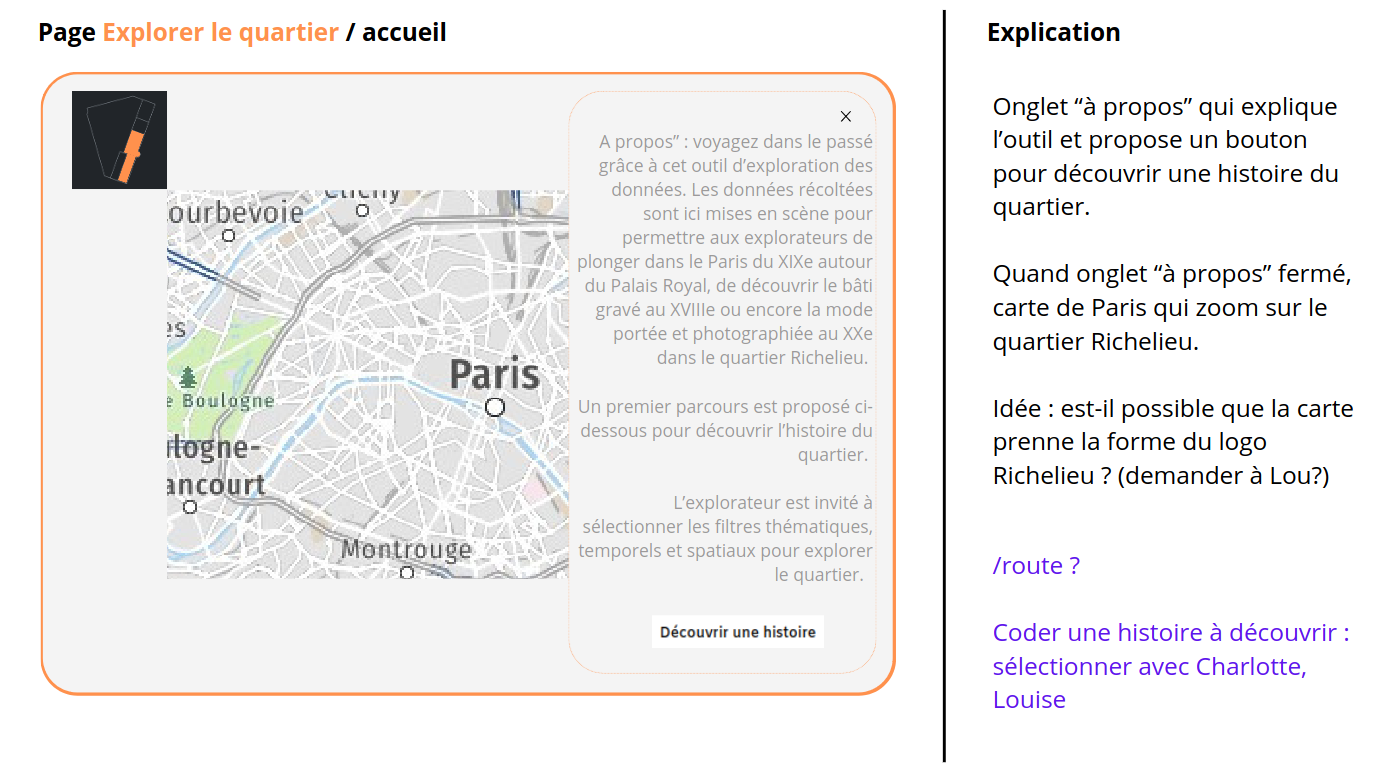
\includegraphics[width=1\linewidth]{images/storyboard-apropos.png}
    \caption{Storyboard page \enquote{à propos}}
    \label{fig:story-propos}
\end{figure}

\subsubsection{Le temps : la chronologie}\label{sous-sous-section:chrono}
Le temps est une notion intrinsèque au projet Richelieu. Sa représentation graphique prend plusieurs formes dont la première, plus conventionnelle, est une frise chronologique. Partant de 1750 pour s'étendre jusqu'à 1950, elle est liée à tous les documents datés. Plusieurs niveaux de détail peuvent s'ajouter à cette frise. Le premier niveau consiste à choisir une date au sein de cette période. Le curseur placé sur 1834, par exemple, affichera toutes les données qui sont précisément liées à cette date. Toutes les autres données sont exclues et n'apparaissent pas sur la carte. Le deuxième niveau proposé consiste à choisir une période au sein de la frise. Seules les données de la période sélectionnées entre deux curseurs sont affichées, le reste est également exclu. Enfin, le troisième niveau plus complexe à conceptualiser propose une sélection plus détaillée. Ce niveau permet de choisir une période et une date précise au sein de celle-ci. La visualisation graphique des données mettrait en exergue cette distinction (comme le propose la figure \ref{fig:story-chrono}). 
Lors des échanges sur la frise chronologique, des questions émergent. Les chercheurs savent que les données ne s'étalent pas de façon homogène sur toute la période. Certaines dates sélectionnées afficheront un très grand nombre de données et elles risquent d'être écrasées par leur volume. On se demande alors s'il faut distordre la frise chronologique et visuellement signifier cette volumétrie occupée par les données. C'est un point soulevé très intéressant à retenir pour des développements futurs.

\begin{figure}[h!]
    \centering
    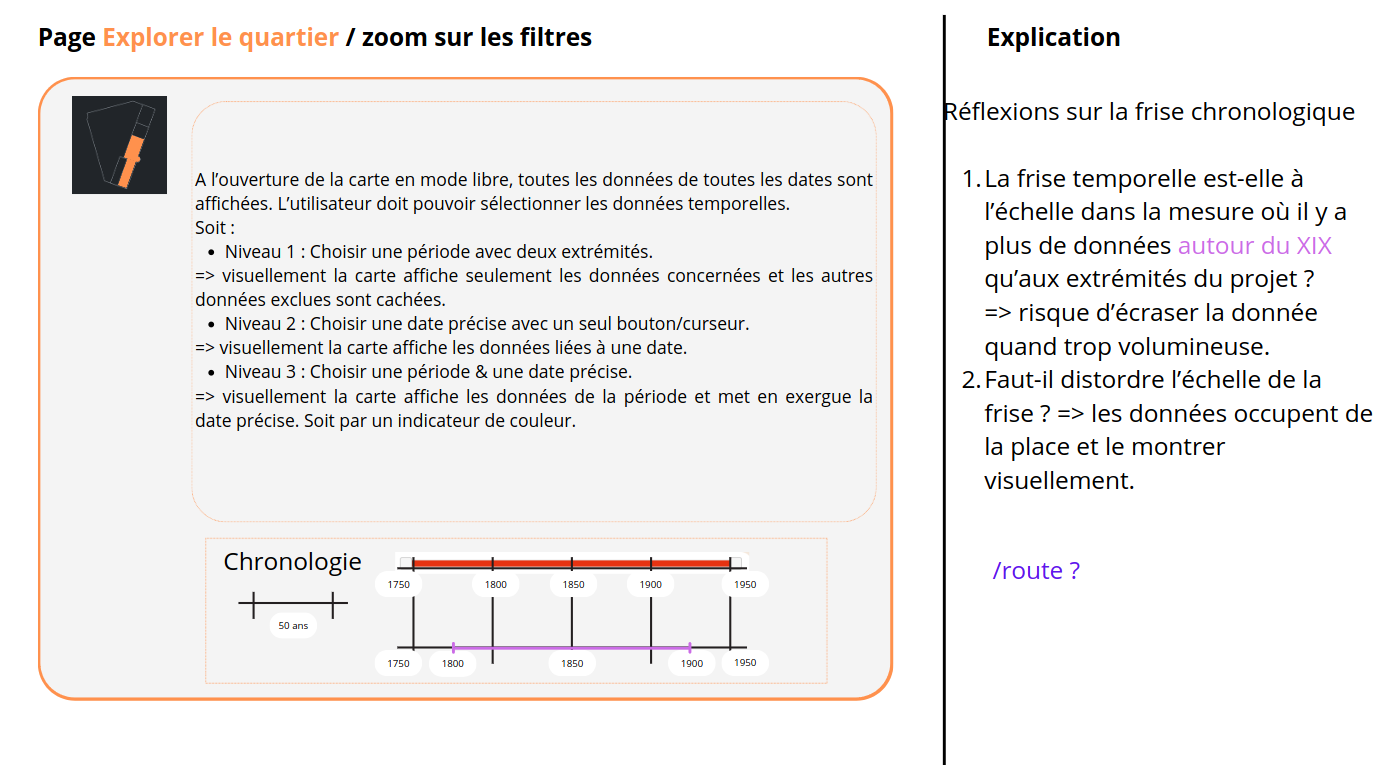
\includegraphics[width=1\linewidth]{images/storyboard-chrono.png}
    \caption{Storyboard page \enquote{chronologie}}
    \label{fig:story-chrono}
\end{figure}

\subsubsection{L'espace : les filtres}
Pour représenter la notion spatiale dans le projet Richelieu, une proposition est de laisser à l'utilisateur la possibilité de choisir le niveau de granularité des données. Nous avons vu que les sources cartographiques sont définies par leur niveau de granularité, parmi lesquels : l'aile, la galerie, l'ensemble et la parcelle. Grâce à un système de filtre à cocher, l'utilisateur peut sélectionner le niveau qu'il souhaite afficher. Ces filtres ont aussi pour objectifs additionnels, combinés entre-eux : c'est-à-dire que tous les niveaux peuvent être affichés, ou seulement un seul ou certains d'entre eux. Ce niveau de granularité ne se mettrait pas à jour en fonction du niveau du zoom car l'échelle du quartier est déjà suffisamment réduite. Cette fonctionnalité a pour but de montrer à l'utilisateur l'évolution parcellaire.

\subsubsection{La double dimension spatio-temporelle : les filtres par fond de carte historique}

L'espace et le temps sont deux dimensions qui, lorsqu'elles sont reliées à la carte, représentent une double dimension spatio-temporelle : l'idée de la spatialisation du temps et de la temporalisation de l'espace. En se faisant se succéder plusieurs cartes historiques, on peut remarquer l'évolution bâtie que ce soit par la construction de nouveaux bâtiments ou par l'ouverture de nouvelles rues. Pour ce faire, nous proposons des filtres à cocher par fond de carte historiques. L'utilisateur pourra, au même titre que les filtres de granularité, sélectionner un ou plusieurs filtres. 

\subsubsection{La sémantique : les filtres thématiques}

Afin de structurer la donnée, nous avons vu que l'équipe réunit les sources documentaires en six grands thèmes: \enquote{Se divertir}, \enquote{Habiter}, \enquote{Consommer}, \enquote{S'habiller}, \enquote{Représenter}, \enquote{S'informer}. Chacun réunit des sous-thèmes appelés \textbf{entités nommées} dans la base de données. L'idée est ainsi de représenter le quartier à travers plusieurs notions sémantiques, que nous envisageons comme autant de filtres thématiques encapsulant les entités nommées regroupées par thèmes. Pour leur visualisation, nous verrons s'ils sont repérés à l'aide de pictogrammes ou plutôt via un système de couleurs.

\begin{figure}[h!]
    \centering
    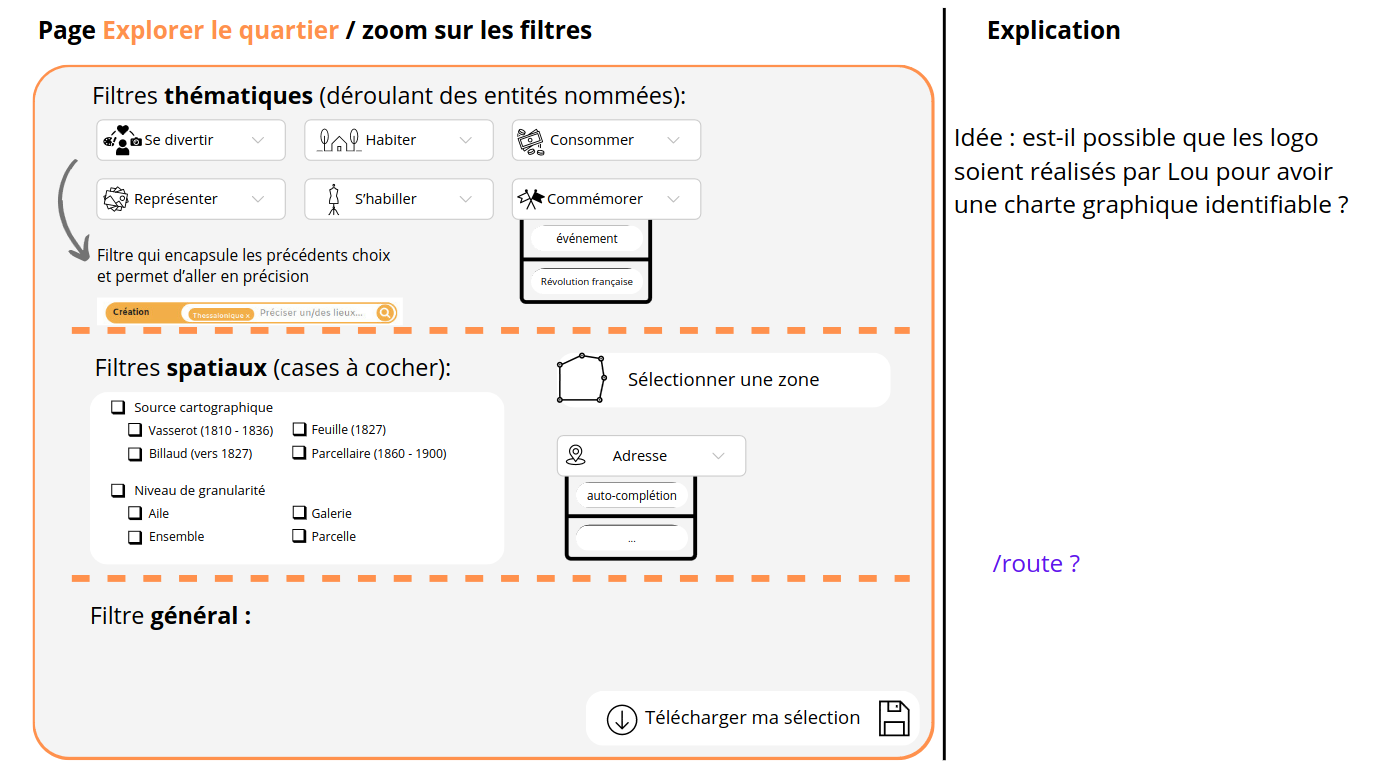
\includegraphics[width=1\linewidth]{images/storyboard-filtres.png}
    \caption{Storyboard page \enquote{filtres}}
    \label{fig:story-filtres}
\end{figure}

\subsubsection{L’iconographie : le carrousel d’images}

Pour représenter l'iconographie, la méthode la plus directe consiste à afficher les images provenant des sources iconographiques. Chaque parcelle étant associée à un ensemble d'iconographies, il est envisagé qu'un carrousel d'images s'affiche lorsqu'un lieu est cliqué sur la carte par l'utilisateur. Toutefois, il existe un risque de saturation de l'espace de visualisation lorsque le nombre d'images liées à un lieu est trop important, certaines images seraient alors inaccessibles car noyées dans une trop large sélection. Les filtres jouent un rôle crucial pour atténuer ce problème. En effet, les iconographies sont accompagnées de métadonnées structurelles et descriptives, qui peuvent être utilisées comme filtres, tels que les thèmes, les dates et les sources cartographiques associées.

La combinaison de l'ensemble de ces filtres permet à l'utilisateur d'afficher les données avec précision. Telle est l'interaction conceptualisée pour la carte. 

\subsubsection{D'autres possibilités}
Toutefois, d'autres possibilités de navigation sont émises lors de réunions de travail. 
\textbf{La barre de recherche} permet de saisir un champ au sein de la carte, telle qu'une adresse, pour afficher instantanément les informations qui y sont liées. Même si cette barre est couramment utilisée sur les sites Web, son développement est particulièrement difficile à mettre en place. Toutefois, elle offre quelques avantages comme l'accès rapide aux données. \textbf{La sélection de zone personnalisée} est une fonctionnalité conçue pour évoquer l'utilisation d'une carte papier, retournée et orientée selon la direction de marche, où les utilisateurs entourent, annotent et crayonnent ce qui les intéresse. Pour reproduire cette matérialité, l'idée est de permettre à l'utilisateur d'interagir directement avec la carte. Les données affichées sont alors exclusivement liées à la zone qu'il a dessinée. Cette fonctionnalité est particulièrement utile pour un chercheur qui, par exemple, se concentre sur un bâtiment spécifique et souhaite accéder uniquement aux informations le concernant. Enfin, la possibilité de \textbf{télécharger les données sélectionnées} depuis une carte permet à l'utilisateur de conserver et d'analyser ces informations en dehors de l'interface initiale. Cela facilite leur utilisation pour des recherches ultérieures. Pour un chercheur, par exemple, cela offre l'avantage de pouvoir manipuler plus en précision les données avec des logiciels spécialisés, favorisant ainsi des analyses plus approfondies que celles permises par la carte. Cette extraction en fonction des besoins spécifiques participe aussi au partage des données. 

\subsubsection{\textit{Quid} du réseau ?}
Les réflexions menées au cours du stage montrent que la notion de « réseau » ne sera pas explicitement représentée sur la carte. Le lieu, en tant qu'entité centrale du projet, est considéré comme la manifestation du réseau, car toutes les informations y sont reliées par la base de données relationnelle. Bien que l'idée d'accompagner la carte d'une visualisation en réseau ait été envisagée, il aurait été nécessaire de déterminer sa pertinence, en se demandant si elle sert à démontrer un propos ou si elle s'inscrit dans une démarche de recherche, selon les distinctions faites par Grandjean.
\\

Les fonctionnalités sus-mentionnées offrent aux utilisateurs, qu'ils soient chercheurs ou novices, une expérience personnalisée et précise. Ces outils ont pour objectif d'offrir une meilleure compréhension du quartier étudié, mais aussi une exploitation approfondie des données. Il convient de rappeler qu'il ne s'agit ici que d'une conceptualisation, définissant des possibilités dont la faisabilité ne sera confirmée qu'au cours du développement informatique. Seule la mise en production permet en effet de déterminer si ces idées peuvent être concrètement réalisées. 

\subsection{Le \textit{MVP} : hiérarchiser les priorités}
Le \textit{Minimum Viable Product}, largement utilisé dans le développement de produits, notamment dans le secteur des technologies, consiste à créer une version simple, basique et fonctionnelle d'un produit, en l'occurrence d'une carte. Après avoir listé les fonctionnalités d'un produit, le  \acrshort{mvp} permet de les hiérarchiser selon un ordre de priorité de développement et d'évaluer la difficulté de leur mise en œuvre pour les développeurs, tout en s'assurant que le produit réponde aux besoins essentiels dès ses premières itérations. L'objectif principal de cette approche est de lancer rapidement un produit fonctionnel pour recueillir des retours d'expérience concrets, afin de vérifier son adéquation avec les attentes des utilisateurs. 

Pour le développement de la carte dans le cadre du projet Richelieu, un  \acrshort{mvp} (voir \ref{fig:mvp}) a été adopté pour clarifier les fonctionnalités, les structurer dans le temps, et garantir une progression méthodique vers la version finale de la géodatavisualisation. Cette approche permet non seulement de tester la carte dès les premières phases de son développement, mais aussi d'affiner ses fonctionnalités en fonction des retours, tout en respectant les contraintes du projet. Le  \acrshort{mvp} sert ainsi de feuille de route, permettant de suivre l'avancement du développement à chaque étape. Les fonctionnalités en orange sont considérées comme réalisables avec un effort minimal et un faible impact pour le projet final. Elles seront probablement développées en priorité dans les premières étapes du projet informatique. Les fonctionnalités en vert sont les éléments essentiels, les \textit{must have} du projet, dont la réalisation a un impact fort et demande un effort de développement acceptable. En rouge sont indiquées les fonctionnalités hors de notre portée de réalisation, telle que la version multilingue. Enfin, en bleu sont les fonctionnalités supplémentaires mais non essentielles au projet, incluant la sélection de zones personnalisées, le téléchargement des données sélectionnées et le parcours guidé. 

\begin{figure}[h!]
    \centering
    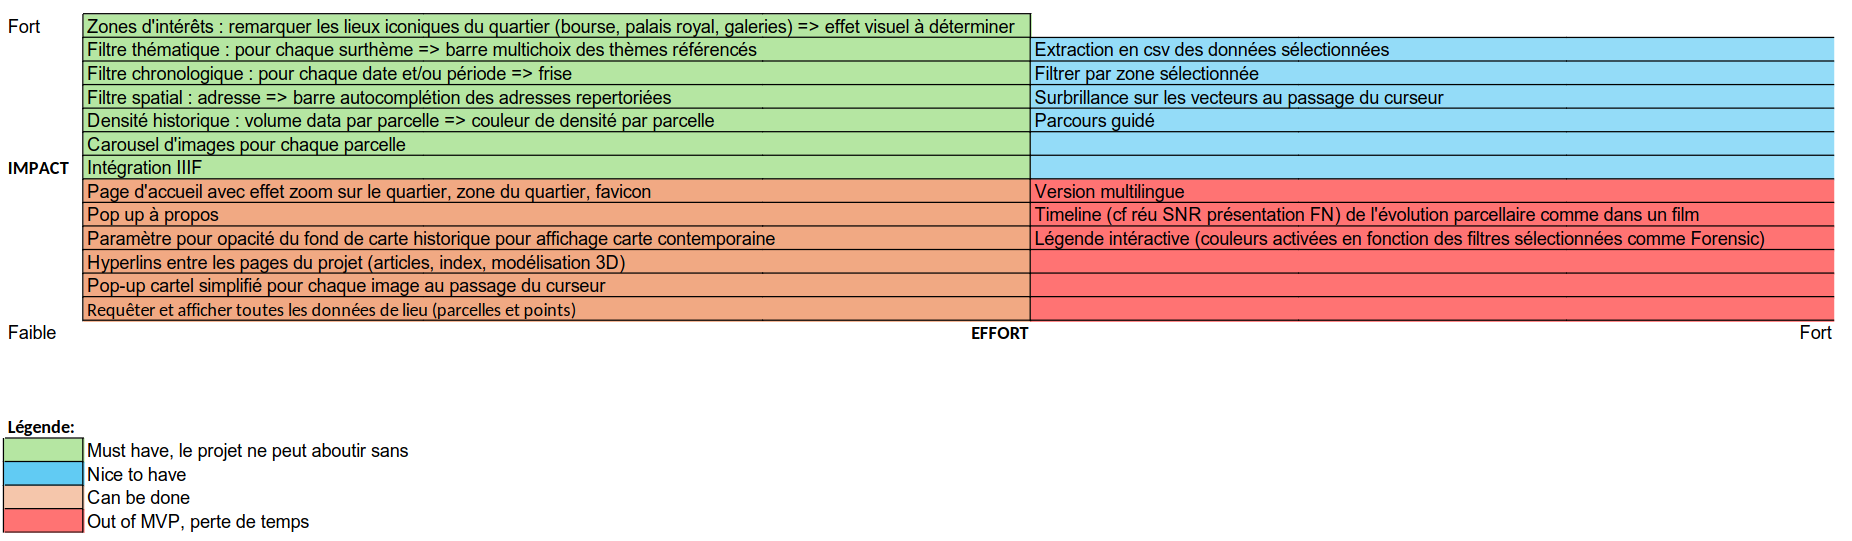
\includegraphics[width=1\linewidth]{images/MVP.png}
    \caption{ \acrshort{mvp} du projet Richelieu}
    \label{fig:mvp}
\end{figure}

Grâce au  \acrshort{mvp} et au \textit{Storyboard}, à considérer comme des outils de gestion du temps, notre feuille de route de développement s'est précisée et il convient de l'exécuter méthodiquement. 

%%%%%%%%%%%%%%%%%%%%%%%%%%%%%%%%%%%%%
% SECTION %%%%%%%%%%%%%%%%%%%%%%%%%%%
\section{Analyser la matérialité de la donnée contre l'effet « boîte noire ».}
La partie précédente du mémoire a exposé la structure de la base de données du projet Richelieu, nous permettant de comprendre comment les corpus sont transformés en données. Dans le chapitre actuel, nous avons également précisé la manière dont nous souhaitons représenter ces données sur la carte. En d'autres termes, nous avons une vision claire des données en entrée et de leur représentation en sortie. Cependant, avons-nous une \textit{overview} sur le contenu de la base de données dans toute sa complexité ? La visualisation graphique que nous observerons sur la carte est-elle réellement fidèle au contenu de la base ? Par exemple, si la carte indique qu'une parcelle est associée à 1000 images, comment savoir s'il s'agit d'une aberration ou d'un résultat authentique ? Jusqu'à quel point pouvons-nous faire confiance aux données visualisées ?  Est-ce que les données affichées sur la carte ont un sens ? Dans quelle mesure la carte invisibilise un récit sur le quartier et inversement ? 

Une analyse en profondeur de la matérialité des données évite l'effet \enquote{boîte noire} et permet de connaître leur volume, leur contenu et leurs particularités. Ce besoin est d'autant plus vrai lorsque l'ingénieur n'a pas conçu la base de données mais qu'il doit interagir et produire à partir de celle-ci. Pour cette étape, il s'agit de rendre visible ce qui est opaque. Ce travail est une précaution, permettant de savoir si la carte reflète les données de manière aussi précise et transparente que possible, minimisant ainsi les risques de biais ou d'erreurs dans la visualisation.

Pour ce faire, il s'agit ici de présenter une analyse comparative et quantitative des données. La base de données est interrogée grâce à un ensemble de requêtes  \acrshort{sql} générées sur pgAdmin\footnote{Voir annexes \ref{chapter:sql}} qui propose également un \textit{plugin} pour visualiser graphiquement les résultats. Les requêtes ne sont pas réalisées par corpus documentaire mais par dimension et point d'accès à la donnée sur la carte : le lieu, les sources documentaires et le temps. 

\subsection{Le lieu}\label{sous-section:lieu}
Nous avons montré que le lieu est l'entité centrale du projet. Toute information est donc reliée à un lieu, voire un groupe de lieux, sinon un document iconographique ou cartographique alors par la suite relié au lieu. 

\subsubsection{La répartition des sources par lieu}\label{sous-sous-section:rm19}

\begin{figure}[!]
    \centering
    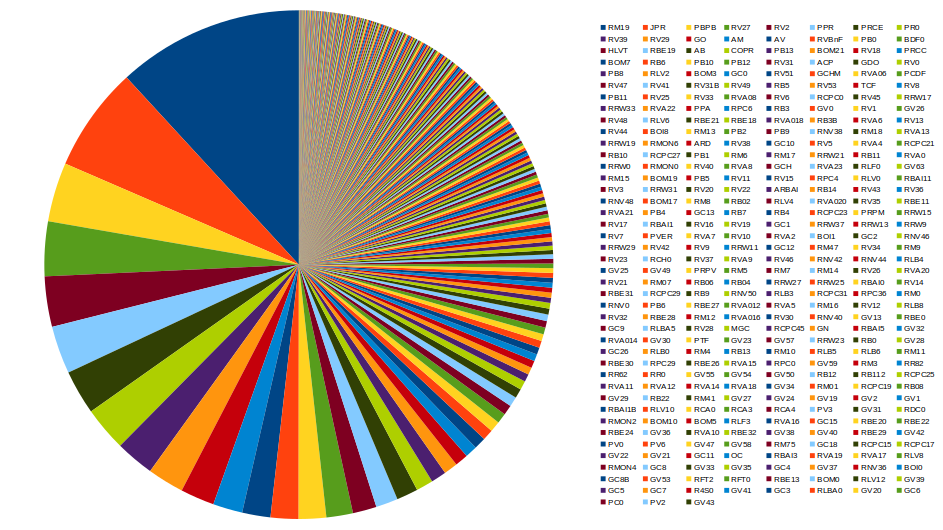
\includegraphics[width=1\linewidth]{images/graphiques/total_sources_lieu.png}
    \caption{La répartition totale des sources par lieu}
    \label{fig:répartition_totale_sources_lieu}
\end{figure}

La légende de ce graphique en camembert (figure \ref{fig:répartition_totale_sources_lieu}) est difficile à lire à cette échelle, il faut simplement retenir que chaque ligne de couleur représente un lieu différent. Le total des sources cartographiques par lieu a été calculé et additionné au nombre total de sources iconographiques par lieu pour donner un nombre total de sources par lieu. Celui-ci est représenté par le volume occupé par chaque part de couleur dans le graphique. On constate distinctement que la répartition du nombre de sources par lieu est loin d'être homogène. En effet, la moitié des sources se concentre sur seulement 14 des 331 lieux répertoriés par le projet. Autrement dit, 50\% des sources sont concentrées sur seulement 4,2\% des lieux, dont un quart seulement est associé à 4 lieux. Plus précisément, un lieu saute aux yeux, il s'agit de la part en bleu marine, le \enquote{RM19}, situé au 19, rue Montpensier et associé au Théâtre du Palais Royal (dont l'adresse a évolué au fil du temps). Il répertorie à lui seul 877 documents. Lieu emblématique de la culture parisienne, il est aussi producteur d'une abondante documentation liée au théâtre, notamment des affiches et des recueils de costumes d'acteurs et actrices, chaque recueil comptant en moyenne 200 pages. Par ailleurs, force est de constater que l'autre moitié des sources est répartie sur les 317 lieux restants, mais cette répartition est également inégale, comme le montre le graphique en barres suivant.

\subsubsection{La répartition des sources iconographiques (> 100) par lieu}
\begin{figure}[ht!]
    \centering
    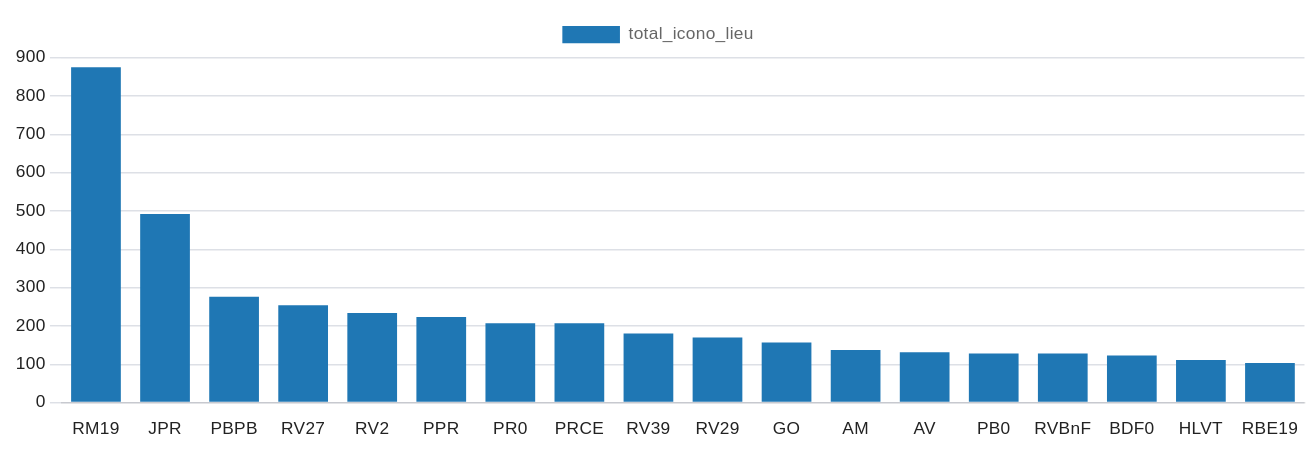
\includegraphics[width=1\linewidth]{images/graphiques/nb_icono_lieu_>100.png}
    \caption{Nombre d'iconographie par lieu (au moins 100)}
    \label{fig:répartition_totale_icono_lieu}
\end{figure}
Ce graphique (\ref{fig:répartition_totale_icono_lieu}) indique par ordre décroissant les lieux ayant plus de 100 sources iconographiques répertoriées.  À la lecture des lieux, on observe une représentation majoritaire de certaines zones géographiques. Les termes \enquote{JPR}, \enquote{PPR}, \enquote{PR0} et \enquote{PRCE} se rapportent tous au Palais Royal, que ce soit à son jardin, à l'ensemble architectural, à la place ou encore au Conseil d'État. De même, \enquote{PBPB} et \enquote{PB0} désignent la Place de la Bourse et le Palais Brongniart. Enfin, \enquote{RV} fait référence à la rue Vivienne. Ces trois lieux apparaissent clairement comme des points d'intérêt largement documentés dans le corpus iconographique, avec la rue Vivienne formant un axe central menant aux deux palais. Notons que les échelles de ces lieux sont différentes : certains sont des bâtiments, tandis que d'autres sont des ensembles viaires ou architecturaux. Or la question se pose de savoir comment éviter d'écraser les données lors de leur visualisation tout en respectant ces différentes échelles de représentations.

\subsubsection{Le nombre de sources cartographiques par lieu}
En ce qui concerne la répartition du nombre de sources cartographiques par lieu, une représentation dans un graphique en barre (\ref{fig:répartition_totale_carto_lieu}) est peu pertinent. On constate simplement que tous les lieux ont au moins une source cartographique. Pour comprendre combien de lieux sont référencés à une ou plusieurs sources cartographiques, le graphe en camembert ci-dessous (\ref{fig:repartition_carto_lieu}) donne à constater que 193 lieux sont référencés à une seule source cartographique, 113 en ont 2, 24 en ont 3 et seulement un lieu, le 17, rue Vivienne (\enquote{RV17}) est référencé dans les 4 sources cartographiques géoréférencées du projet. Très peu de lieux ont une couverture cartographique dense. Cela suggère une documentation partielle de l'évolution parcellaire, probablement liée à la stabilité de certains lieux, comme indiqué dans la méthode régressive évoquée précédemment (\ref{par:méthodes}).

\begin{figure}[ht!]
    \centering
    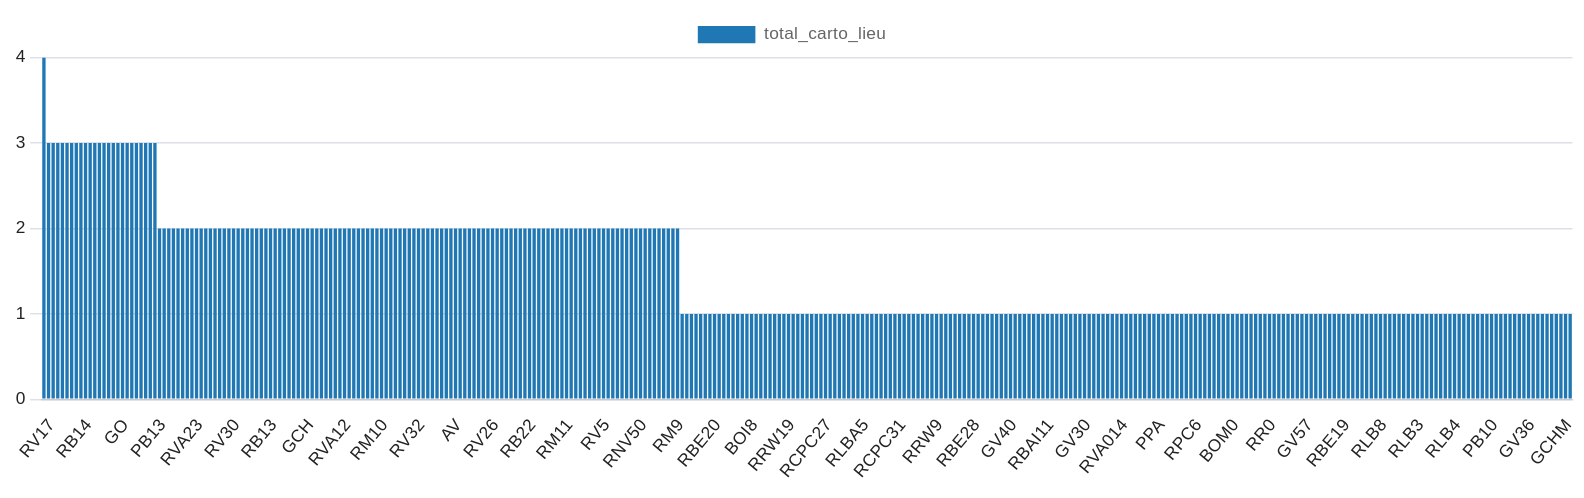
\includegraphics[width=1\linewidth]{images/graphiques/nb_carto_lieu_barChart.png}
    \caption{Nombre de cartographies par lieu}
    \label{fig:répartition_totale_carto_lieu}
\end{figure}

\begin{figure}[ht!]
    \centering
    
\includegraphics[width=0.8\linewidth]{images/graphiques/repartition_lieux_nb_carto_lieu_pie.png}
    \caption{Répartition totale des lieux par source cartographique par lieu.}
    \label{fig:repartition_carto_lieu}
\end{figure}

En résumé, cette première analyse met en évidence une concentration marquée des sources iconographiques et cartographiques sur un nombre restreint de lieux, avec une répartition inégale. Bien que certains affichages nous apparaissent comme aberrants, il convient d'indiquer que certains types de graphiques illustrent mieux les données que d'autres. En réalité, il s'agit d'une distribution déséquilibrée des sources par lieu.  Cette observation est essentielle à garder à l'esprit lors du développement afin d'éviter toute distorsion des données et de garantir une représentation fidèle et équilibrée du patrimoine étudié.

\subsection{Les corpus documentaires}
Les corpus documentaires du projet sont aussi un point d'entrée dans l'application. Intéressons-nous à la provenance de la majorité des sources et aux principaux médiums 

\subsubsection{La répartition des sources par institution}
Identifier les principales sources du projet Richelieu, c'est-à-dire les lieux de conservation des documents iconographiques et cartographiques, permet d'évaluer si la base de données reflète véritablement les ambitions initiales du projet. L'analyse révèle que les sources proviennent de 26 institutions différentes, mais près de 83\% d'entre elles sont concentrées dans seulement quatre institutions : le Musée Carnavalet (1333 sources), la \acrshort{bnf} (1312 sources), les bibliothèques spécialisées de la ville de Paris (928 sources), et la Bibliothèque historique de la ville de Paris (827 sources). Quant aux sources cartographiques, elles sont principalement issues de centres d'archives. 
\begin{figure}[ht!]
    \centering
    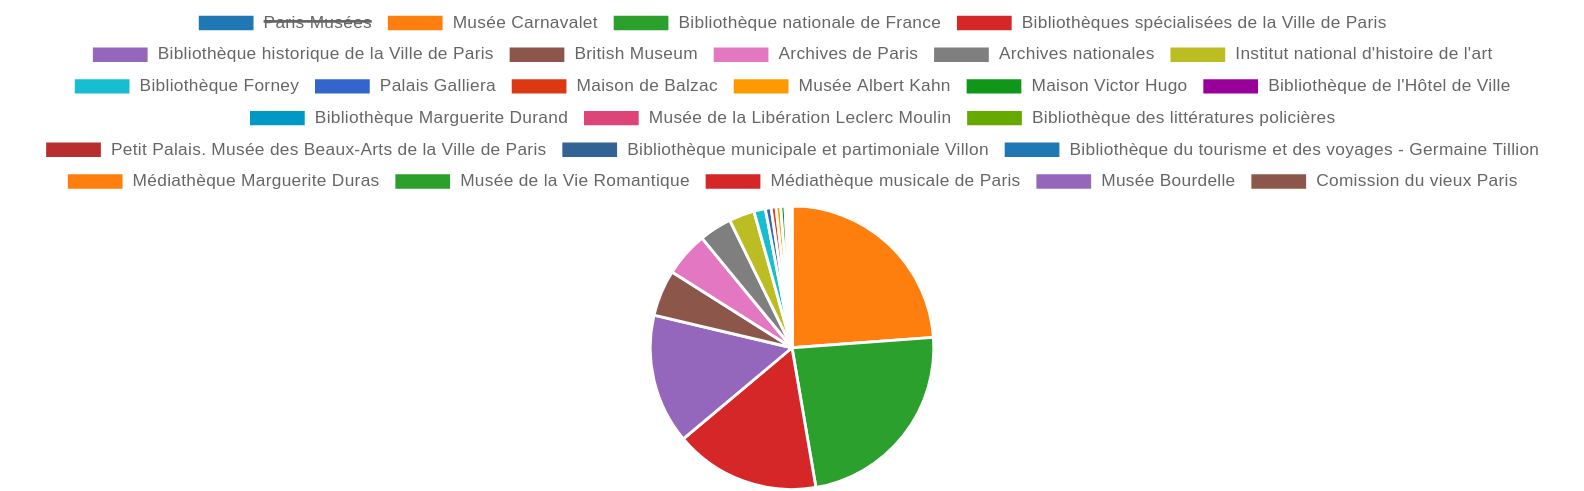
\includegraphics[width=1\linewidth]{images/graphiques/total_sources_institution.png}
    \caption{Nombre de sources par institution (1/2)}
    \label{fig:sources_institution}
\end{figure}
\begin{figure}[ht!]
    \centering
    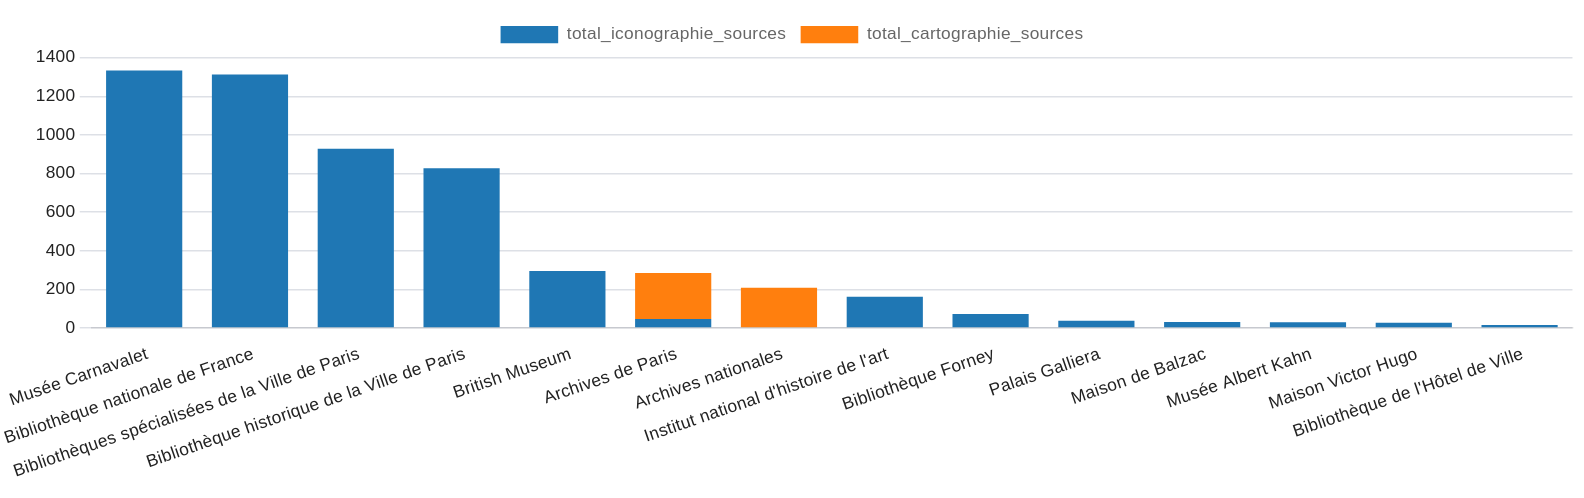
\includegraphics[width=1\linewidth]{images/graphiques/total_source_institution.png}
    \caption{Nombre de sources par institution (2/2)}
    \label{fig:sources_institution2}
\end{figure}
Ainsi, la majorité des données historiques du projet ne proviennent pas des principaux acteurs, à l'exception notable de la \acrshort{bnf}. Pourtant, l'une des motivations premières du projet était de découvrir l'histoire à travers les collections de ces institutions, elles-mêmes porteuses du projet. Il se pourrait que ce résultat soit influencé par les politiques de numérisation variables selon les institutions ou par le lien spécifique des collections avec le quartier concerné.

\subsubsection{La répartition des iconographies par medium}
Identifier la répartition des médiums au sein du corpus iconographique donne à voir d'autres caractéristiques du corpus.

\begin{figure}[ht!]
    \centering
    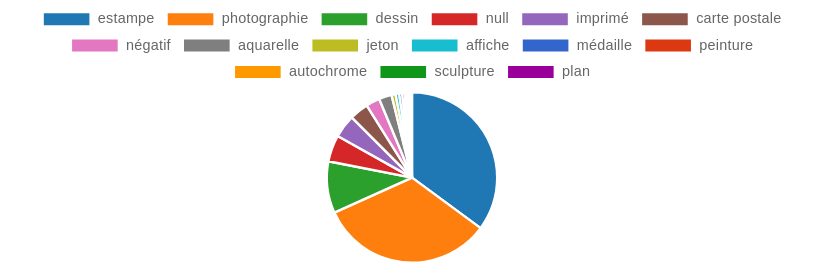
\includegraphics[width=1\linewidth]{images/graphiques/nb_icono_technique>10.png}
    \caption{Répartition des iconographies par technique}
    \label{fig:icono_technique}
\end{figure}

On constate que la majorité des documents iconographiques rassemblés dans le projet sont des estampes et des photographies, deux médiums qui ont joué un rôle central dans la représentation visuelle au XIX\ieme~ siècle et au XX\ieme~ siècle respectivement. Cette prédominance s'explique non seulement par leur importance historique, mais aussi par les choix de numérisation effectués par les institutions patrimoniales. En effet, la numérisation d'estampes et de photographies est techniquement plus simple et moins coûteuse que celle d'œuvres d'art plus fragiles comme les peintures, les sculptures ou les autochromes, qui nécessitent des techniques de capture plus sophistiquées et des traitements spécifiques. Par conséquent, la composition de cette collection numérisée reflète à la fois les priorités historiques et les contraintes techniques des institutions en matière de conservation numérique.

\subsection{Le temps}
Pour le projet Richelieu, le temps est une dimension à faire figurer dans la visualisation des données historiques. Dans le cadre d'un projet visant à explorer des périodes historiques, à remonter dans le temps en somme, il est essentiel d'examiner attentivement la répartition temporelle des sources disponibles.

\subsubsection{La répartition temporelle des sources : par intervalle de 50 ans}
Ce graphique (\ref{fig:total_sources_date50}) met en évidence une répartition inégale des sources selon des intervalles de 50 ans. Le XIX\ieme~ siècle est largement représenté avec un nombre significatif de sources, en particulier durant la seconde moitié du siècle. En revanche, le XX\ieme~ siècle et le XVIIIe siècle sont moins bien représentés en termes de volume de sources. Cette disparité s'explique probablement par plusieurs facteurs qui échappent à la sélection intentionnelle des chercheurs. Le XIX\ieme~ siècle a vu une intensification de la production d'informations, notamment grâce aux progrès des techniques de reproduction initiés par la révolution industrielle, qui ont également favorisé l'essor du journalisme et de la photographie. À l'inverse, le XVIIIe siècle est moins représenté, car les techniques de reproduction de l'époque étaient principalement artisanales, et non industrielles, ce qui a limité la production et la préservation des documents. Pourtant, on pourrait hâtivement penser que les sources deviennent plus abondantes avec l'avancée du temps, et le développement des techniques de reproduction de l'information ainsi que celles de conservation.
\begin{figure}[ht!]
    \centering
    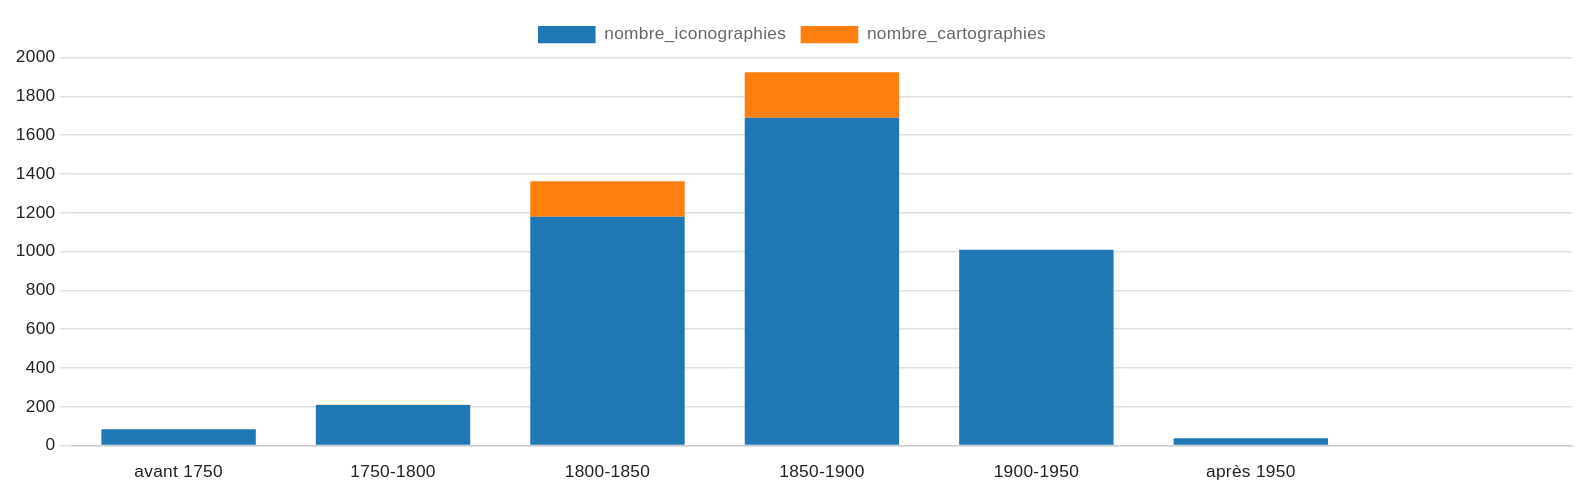
\includegraphics[width=1\linewidth]{images/graphiques/total_source_date_50.png}
    \caption{Nombre total de sources par date (intervalle de 50 ans)}
    \label{fig:total_sources_date50}
\end{figure}
Un point surprenant soulevé par le graphique est la présence de documents qui dépassent les bornes chronologiques initialement définies pour le projet. On trouve en effet une petite proportion de documents datant d'avant 1750 et d'après 1950. Cette anomalie soulève des questions quant à la pertinence de leur inclusion. Il serait intéressant de demander aux chercheurs de justifier leur présence et de déterminer si leur intégration dans la frise chronologique est vraiment nécessaire ou si ces documents pourraient être retirés pour mieux respecter les bornes temporelles du projet.

\subsubsection{La répartition temporelle des sources : par intervalle de 10 ans}
\begin{figure}[ht!]
    \centering
    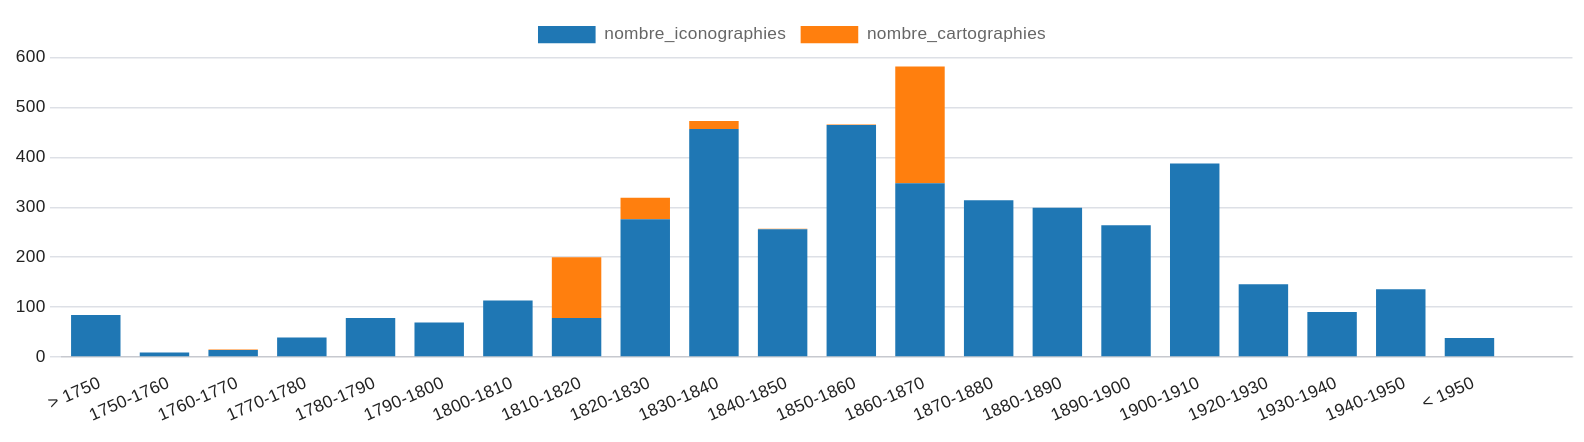
\includegraphics[width=1\linewidth]{images/graphiques/total_source_date_10.png}
    \caption{Nombre total de sources par date (intervalle de 10 ans)}
    \label{fig:total_sources_date10}
\end{figure}
L'analyse à une échelle plus fine permet de révéler des nuances importantes dans la répartition des sources. Par exemple, il est particulièrement surprenant de constater que le nombre de sources datant d'avant 1750 dépasse celui des sources comprises entre 1750 et 1780. Ces sources antérieures pourraient ainsi compenser le déficit observé pour certaines périodes couvertes par le projet. De manière générale, on observe une concentration des sources sur un XIX\ieme~ siècle élargi, qui commence avec la Révolution française et s'étend jusqu'à la veille de la Première Guerre mondiale.

Cependant, une telle visualisation des données présente certains biais interprétatifs. Elle pourrait induire en erreur en suggérant que le projet adopte une approche historiographique particulière, alors même que ce postulat n'a pas été explicitement formulé au début des études sur le quartier Richelieu. De plus, cette visualisation peut donner l'impression que le projet présente des lacunes en sources cartographiques, notamment à partir de la seconde moitié du XIX\ieme~ siècle. Or, il est important de noter que les sources cartographiques sont souvent rattachées à des périodes spécifiques en fonction de la réalité bâtie, ce qui signifie qu'un bâtiment, une fois cartographié, peut ne pas nécessiter de nouvelles cartographies tant qu'il reste inchangé. Par exemple, un bâtiment construit en 1800 apparaîtra sur un plan de 1812 et pourrait rester inchangé jusqu'à aujourd'hui, mais sa présence dans la base de données sera seulement répertoriée dans l'intervalle 1810-1820, selon la date de création du dit plan. Enfin, le graphique omet de mentionner les données non datées, ou \enquote{NULL}, qui ne sont pas représentées ici. Le résultat de la requête \acrshort{sql} en donne pourtant 333, et leur exclusion pourrait également influencer la compréhension globale de la répartition des sources dans le projet.  

Cette étape de travail n'a pas pour objectif de mettre en lumière d'éventuelles lacunes du projet en termes de volume de données ou de répartition, mais plutôt de comprendre les raisons sous-jacentes et d'identifier des explications. Elle m'a permis de saisir comment la recherche a été menée, quels sont les principaux intérêts des chercheures et, surtout, comment la recherche a été traduite en données concrètes dans la base de données.

L'analyse du contenu de cette base résulte d'un travail long et manuel que j'ai personnellement accompli, mais la partie suivante permettra de souligner qu'une méthode de validation des données, qu'elle soit automatisée ou hybride, pourrait simplifier ce processus.

\subsection{Une méthode recommandée : mise en place de processus hybrides de validation}

Pour garantir la qualité et la fiabilité des données affichées, il est pertinent d'adopter des processus de validation combinant automatisation et intervention humaine, autrement dit, des méthodes hybrides. Cette approche permet d'allier l'efficacité des processus automatisés avec la précision et le discernement de l'analyse manuelle, assurant ainsi une validation plus rapide et plus fiable des données.

La mise en place de scripts de validation constitue un élément central de cette méthode. Ces scripts pourraient effectuer des contrôles systématiques, tels que la détection de valeurs manquantes, la vérification de la conformité des formats de données (comme les dates ou les coordonnées géographiques), et l'identification de doublons. Ils pourraient également évaluer la densité des données par catégorie, période ou lieu, ce qui permettrait de repérer les déséquilibres ou les lacunes susceptibles de biaiser les analyses, comme nous l'avons précédemment exposé. 

Toutefois, ces contrôles automatisés doivent être complétés par une validation manuelle qui interroge directement la base de données via l'interface graphique du  \acrshort{sgbdr} afin de garantir un contrôle robuste des données et d'offrir par ailleurs des indications précieuses aux utilisateurs. Par exemple, l'ajout d'indicateurs métriques sur la carte pourrait être envisagé. Ainsi, un chercheur serait informé si sa requête ne représente qu'un faible pourcentage du total des données, l'incitant éventuellement à élargir sa recherche. Bien que de tels indicateurs soient parfois mentionnés, l'ensemble de cette méthode de validation exige toutefois un investissement en temps supplémentaire. Cette méthode n'a pas pu être mise en œuvre pour le développement de la carte\footnote{Ce paragraphe est le fruit de discussions avec les membres du SNR, externes au projet, au cours du stage.}. Finalement, la méthode utilisée est une validation croisée qui consiste à comparer les données affichées sur la carte et celles requêtées directement en  \acrshort{sql} sur la base de données. 


Pour conclure, cette analyse approfondie du contenu de la base de données a permis de dégager les principales orientations du projet. Il en ressort que la majorité des documents sont des iconographies provenant du Musée Carnavalet et, plus largement, des collections de l'établissement Paris Musées, couvrant une période s'étendant de 1820 à 1870. Nous remarquons que le volume d'informations n'est pas uniformément réparti sur les deux siècles étudiés dans le cadre du projet. De plus, les différentes couches d'informations varient considérablement d'un lieu à un autre, certaines zones étant beaucoup plus riches en données que d'autres. Ces caractéristiques, tant temporelles que spatiales, ont des implications directes pour la mise en visualisation des données sur la carte. La concentration des sources dans certaines périodes ou dans des lieux spécifiques nécessite une attention particulière lors de la conception de la cartographie, afin de garantir une représentation équilibrée et fidèle des données. Il s'agit de se demander comment éviter de sur-représenter certaines périodes ou certains lieux, au détriment d'autres, et de veiller à ce que la carte reflète avec précision la réalité complexe et parfois déséquilibrée des sources historiques. 
Nous pensons que c'est en tenant compte de ces disparités que le potentiel exploratoire de la carte pourra pleinement s'exprimer. La carte ne se contentera pas d'être un simple outil de visualisation, mais elle dévoilera également les dynamiques historiques et spatiales sous-jacentes, permettant une interprétation plus riche et instructive des données. La carte serait \textit{démonstration} et \textit{recherche}. Cette approche transforme la carte en un instrument d'exploration du patrimoine étudié, en tenant compte  des spécificités et des biais propres à la base de données.

\subsubsection{Conclusion du chapitre}
Grâce à ce chapitre, nous avons vu que la définition des objectifs de développement spécifiques à la visualisation des données par cartographie Web est essentielle et antérieure à l'étape de développement. Elle permet notamment d'assurer la cohérence et l'orientation de la carte afin que celle-ci corresponde aux axes de recherche du projet. Cela permet de gagner en précision sur les fonctionnalités à développer, les données à intégrer, les choix techniques à privilégier. Les besoins des publics visés (novices ou experts) sont aussi à recueillir dans la mesure du possible. Cette étape permet aussi de comprendre le contexte de production des cartographies Web dans lequel le projet s'inscrit.

%%%%%%%%%%%%%% CHAPT 4 %%%%%%%%%%%%%%%%%%%%%%%%%%%%%%%%%%
\chapter{La réalisation technique : le développement Web \textit{full-stack}}
\chaptermark{Réaliser l'outil}
% PARTIE 2 - TECHNIQUE %%%%%%%%%%%
% CHAPITRE 4 %%%%%%%%%%%%%%%%%%%%%
%%%%%%%%%%%%%%%%%%%%%%%%%%%%%%%%%%
Ce quatrième chapitre décrit le développement \textit{full-stack} de la carte, organisé en trois étapes. La première étape consiste à établir les fonctionnalités structurelles de la carte, incluant le fond de carte par défaut, le cartouche de la carte (titre, échelle, source, etc.), ainsi que les onglets destinés à accueillir les filtres, les images et la légende. Cet ensemble est réalisé à partir des fonctionnalités de la librairie Leaflet qu'il conviendra de définir. À ce stade, la carte n'est pas encore connectée à la base de données. La deuxième étape consiste à établir cette connexion via une \acrshort{api}, ce qui inclut la présentation de son fonctionnement et du requêtage asynchrone de l'application. L'\acrshort{api} permet ainsi de transmettre les données depuis la base jusqu'au \textit{front-end}. Une fois que les données sont prêtes pour être liées à la carte, elles doivent être réceptionnées et formatées pour être affichées et ordonnées afin de permettre à l'utilisateur une exploration interactive du projet Richelieu.  Il est important de noter que les propositions proposées dans ce chapitre sont provisoires, elles sont à l'état de brouillon. La carte présentée lors de la soutenance pourrait différer de celle présentée au cœur de ce chapitre, car le stage se termine après la date de soumission du mémoire.


%%%%%%%%%%%%%%%%%%%%%%%%%%%%%%%%%%%
% SECTION %%%%%%%%%%%%%%%%%%%%%%%%%
\section{Les fonctionnalités structurelles}
La carte est structurée en plusieurs éléments qui permettent son bon fonctionnement et son interaction avec l'utilisateur. Les modules qui la constituent sont développés avec la librairie Leaflet. 
% SUBSECTION %%%%%%%%%%%%%%%%%%%%%%%%%
\subsection{La librairie Leaflet}
\subsubsection{Définition et avantages}
Le projet Richelieu a fait le choix d'utiliser la librairie Leaflet pour réaliser la carte car elle présente plusieurs avantages. Il s'agit d'une bibliothèque JavaScript \textit{open source} conçue pour créer des cartes interactives. Les cartes créées en Leaflet sont compatibles avec les principaux navigateurs Web et adaptées aux environnements mobiles. La librairie est bien documentée par une communauté internationale\footnote{Le \href{https://leafletjs.com/plugins.html}{site} réunit une documentation très riche.} et active qui contribue à son amélioration. Leaflet est surtout connue pour sa prise en main facile pour tout développeur débutant : une simple carte Web peut être créée en quelques lignes de code. Parmi ses autres avantages, la librairie Leaflet est légère (le fichier JavaScript principal ne pèse que 42 kilooctets)\footnote{En informatique, la légèreté d'une librairie est importante car un fichier plus léger se charge plus rapidement dans le navigateur.} et performante (elle peut gérer des grandes quantités de données géospatiales sans surcharger les ressources du navigateur) car elle garantit des temps de chargement des données rapides. Sa flexibilité permet aussi l'intégration de nombreuses fonctionnalités grâce à des \textit{plugins} référencés sur le site de la librairie. Plusieurs zoom, des \textit{popups} ou encore les couches vectorielles sont possibles. Grâce à \acrshort{css}, ces éléments d'interface peuvent être facilement adaptés aux besoins graphiques de chaque projet. Ces avantages rendent Leaflet particulièrement adapté aux projets nécessitant des cartes interactives performantes et modulaires comme c'est le cas du projet Richelieu. 

\subsubsection{D'autres librairies et inconvénients}
Toutefois, il existe plusieurs librairies comparables à Leaflet pour la création de carte interactive sur le Web, mais elles présentent divers inconvénients. Par exemple, rares sont les librairies entièrement gratuites. L'\acrshort{api} JavaScript de Google Maps permet d'intégrer des cartes dans une application mais elle n'est pas \textit{open source}. MapBox GL JS offre une version gratuite, mais avec des fonctionnalités limitées. D'autres, comme OpenLayers et D3.js pour les plus connues, sont des librairies gratuites et complètes (riches en fonctionnalités et supportent de nombreux formats de données) mais elles nécessitent une longue courbe d'apprentissage. D3.js est par ailleurs plus orientée pour la visualisation de données au sens large que strictement pour la cartographie. Dans ce contexte, ces bibliothèques présentent des forces pour d'autres projets et des faiblesses pour le projet Richelieu.

Donc même si Leaflet présente plusieurs inconvénients car il n'est pas développé par un géographe et manque ainsi en rigueur, il reste le meilleur choix en raison de sa simplicité et de son adaptabilité pour développer les fonctionnalités qu'il convient à présent de présenter.  

% SUBSECTION %%%%%%%%%%%%%%%%%%%%%%%%%
\subsection{Les fonds de carte}
Toute carte géographique en ligne comporte au moins un fond de carte de référence, qui constitue une couche de base fournissant un contexte visuel et géographique. Ce fond de carte inclut des éléments d'arrière-plan tels que les routes, les limites administratives et les bâtiments. Il est placé en dessous des autres couches, qui viennent s'y superposer, et n'est généralement pas mentionné dans la légende. Les cartes sur le Web fonctionnent selon un système de superposition de couches, similaire aux cartes traditionnelles où l'on superpose un fond topographique avec des maillages administratifs, des frontières, des chemins de randonnée, des infrastructures ferroviaires et routières, ainsi que des espaces bâtis et naturels. Cette approche de modélisation géographique sur papier est transposée à la cartographie Web. 

\subsubsection{Des repères contemporains}
Leaflet propose un fond de carte par défaut mais il est possible de choisir celui qui correspond le mieux à nos besoins. Tandis que certains créent leur propre carte contemporaine, il existe un siteWeb qui recense de nombreux fonds existants (\href{https://leaflet-extras.github.io/leaflet-providers/preview/}{Leaflet Provider}). Certains fonds affichent les informations géographiques et topographiques, comme le détail du relief ou comme les bâtiments en \acrshort{3d} (voir~ le n°4 dans la figure \ref{fig:fond-carte-contemporain}), tandis que d'autres cartes adoptent un style inspiré de l'aquarelle (voir~ le n°5 dans la figure \ref{fig:fond-carte-contemporain}). Dans le cadre du projet Richelieu, nous avons restreint notre choix à quelques options adaptées un fond de carte urbain. Il est en effet essentiel que les rues et certains noms soient visibles, que les espaces verts soient discrètement représentés, et que l'information demeure lisible sans être trop claire ou trop sombre, tout en évitant des contrastes excessifs. 
\begin{figure}[h!]
    \centering
    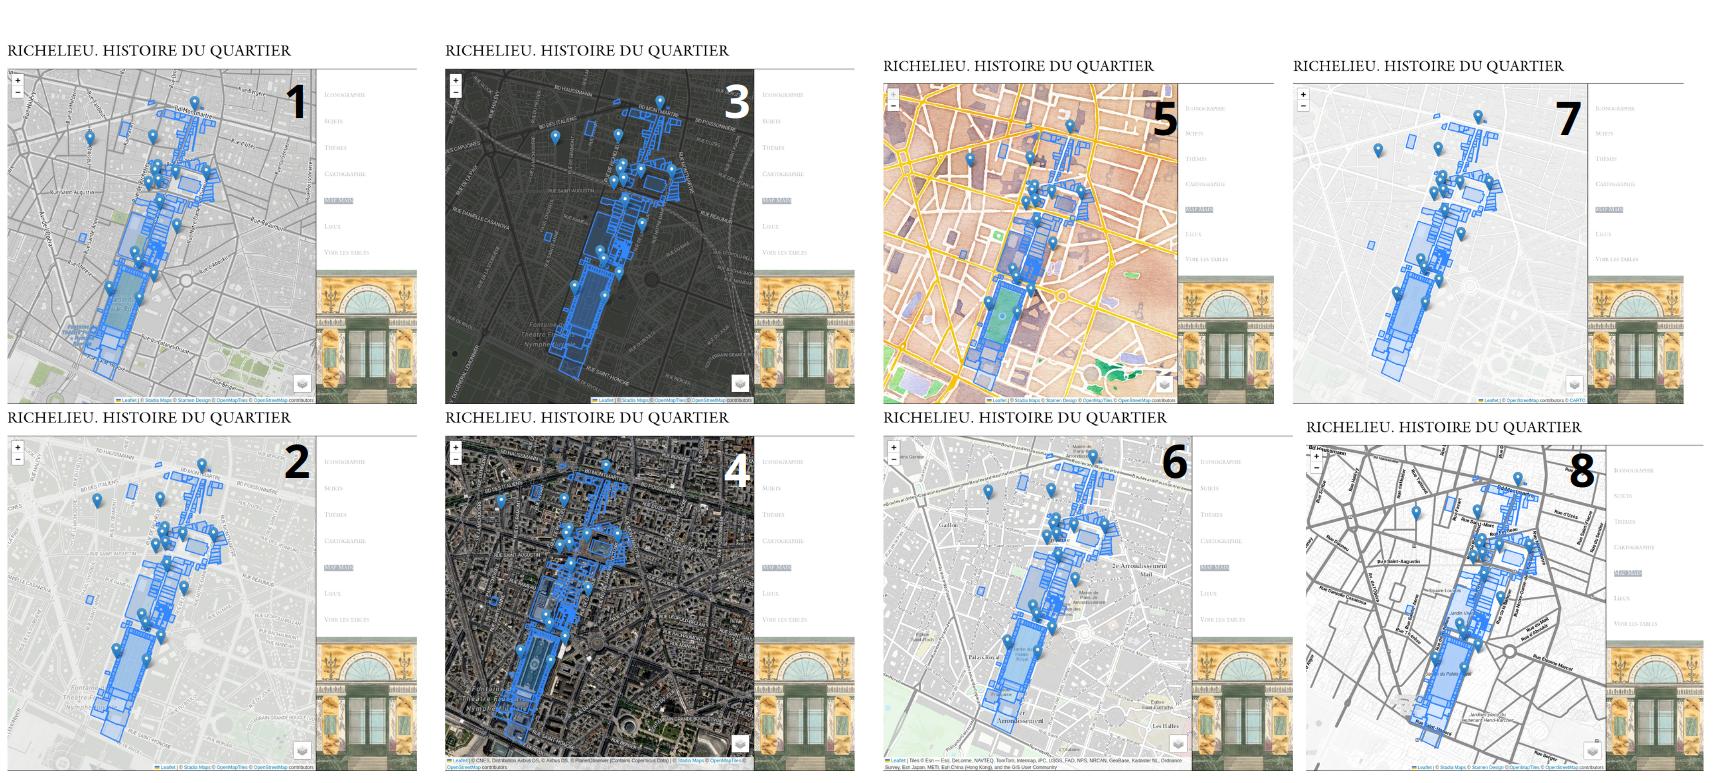
\includegraphics[width=1\linewidth]{images/fond-de-carte-contempo.png}
    \caption{Plusieurs propositions d'un fond de carte contemporain, \mhd.}
    \label{fig:fond-carte-contemporain}
\end{figure}
C'est pourquoi nous avons retenu le fond nommé World Topo Map, le n°6 de la figure \ref{fig:fond-carte-contemporain}. Il offre une bonne lisibilité des noms de rues, boulevards et squares, tout en restant clair. Ce fond de carte est équilibré, il n'y a pas de surcharge d'informations et l'espace n'en est pas trop dépouillé. Il a été conçu par la société internationale \acrshort{esri} (\textit{Environmental Systems Research Institute}), un acteur majeur dans le développement des  \acrshort{sig} appliqués à l'aménagement du territoire. Il est stocké par les serveurs de ArcGIS Online et se matérialise par une \acrshort{url}. Le fond de carte est donc une ressource du Web et externe à notre code mais qu'il convient d'inclure. 

Mais avant de se lancer dans les questions techniques d'ajout de fond de carte, une rapide présentation technique de Leaflet s'oblige. En Leaflet, une carte est stockée dans un objet \texttt{(L.map)} que l'on vient compléter, dans une approche modulaire, en y ajoutant d'autres objets Leaflet: des couches vectorielles, les popups, etc. Les données sont positionnées grâce à leur coordonnées géographiques. Il est ensuite possible de paramétrer des interactions avec la carte (click, scroll...) et donc de définir des scénarii de navigation. Enfin, Leaflet se charge de la production d'une visualisation cartographique en \acrshort{html}, à partir du code JavaScript utilisé pour produire la carte.

En Leaflet, un fond de carte est appelé \texttt{tileLayer} (souvent traduit de manière approximative par \enquote{couche de tuile}). On vient stocker l'\acrshort{url} dans une variable nommée \texttt{contemporain} ci-dessous que l'on ajoute à l'objet carte, \texttt{map}. De cette manière, le fond de carte est visible dès que la carte est chargée, c'est-à-dire dès que la page du navigateur Web est rafraîchie. Il convient de crééer l'objet \texttt{map} avant d'y ajouter une couche d'information.
 \begin{lstlisting}[language=PYTHON, caption=Variables et fonction d'initialisation de la carte en JavaScript]
 var map = L.map('map', {zoomControl:false}).setView([48.866772, 2.338935], 12);    
 
 var contemporain = L.tileLayer(
    'https://server.arcgisonline.com/ArcGIS/rest/services/World_Topo_Map/MapServer/tile/{z}/{y}/{x}', 
    {
        opacity: 1, 
        maxZoom: 18,
        minZoom: 12
    }
).addTo(map); 

 setTimeout(function(){
    map.flyTo([48.866772, 2.338935], 16);
 }, 4000);\end{lstlisting}
 
La création d'une \texttt{tileLayer} implique généralement de définir un niveau de zoom minimal et maximal, ainsi que des paramètres pour centrer la carte sur une localisation spécifique. 
Il est important de noter que Leaflet propose un grand nombre de paramètres, la plupart étant prédéfinis par défaut. Il revient donc au développeur de modifier ces paramètres par défaut afin que les interactions avec la carte correspondent aux spécifications souhaitées. Par exemple \texttt{zoomControl~:~false} désactive les contrôles de zoom par défaut (c'est-à-dire les boutons \enquote{~+~} et \enquote{~-~} que l'on peut généralement apercevoir sur une carte). A la place, il a été décidé de jouer pleinement avec les interactions offertes par Leaflet et JavaScript. 
Dans la première ligne de code, nous reconnaissons des coordonnées géographiques \texttt{48.866772, 2.338935} qui correspondent à un point géographique à Paris. Elles sont accompagnées d'un niveau de zoom \texttt{12} qui offre une vue intermédiaire permettant de visualiser toute la ville de Paris (voir~ \ref{fig:zoom-12}). A l'inverse, la fonction \texttt{setTimeout} augmente le niveau de zoom à \texttt{16} et offre une vue détaillée sur le quartier Richelieu (voir~ \ref{fig:zoom-16}). Cette transition est dynamique donnant un effet de \enquote{vol} vers la destination après 4 secondes d'attente au chargement de la carte.

\begin{figure}[h!]
    \begin{subfigure}{.5\textwidth}
      \centering
      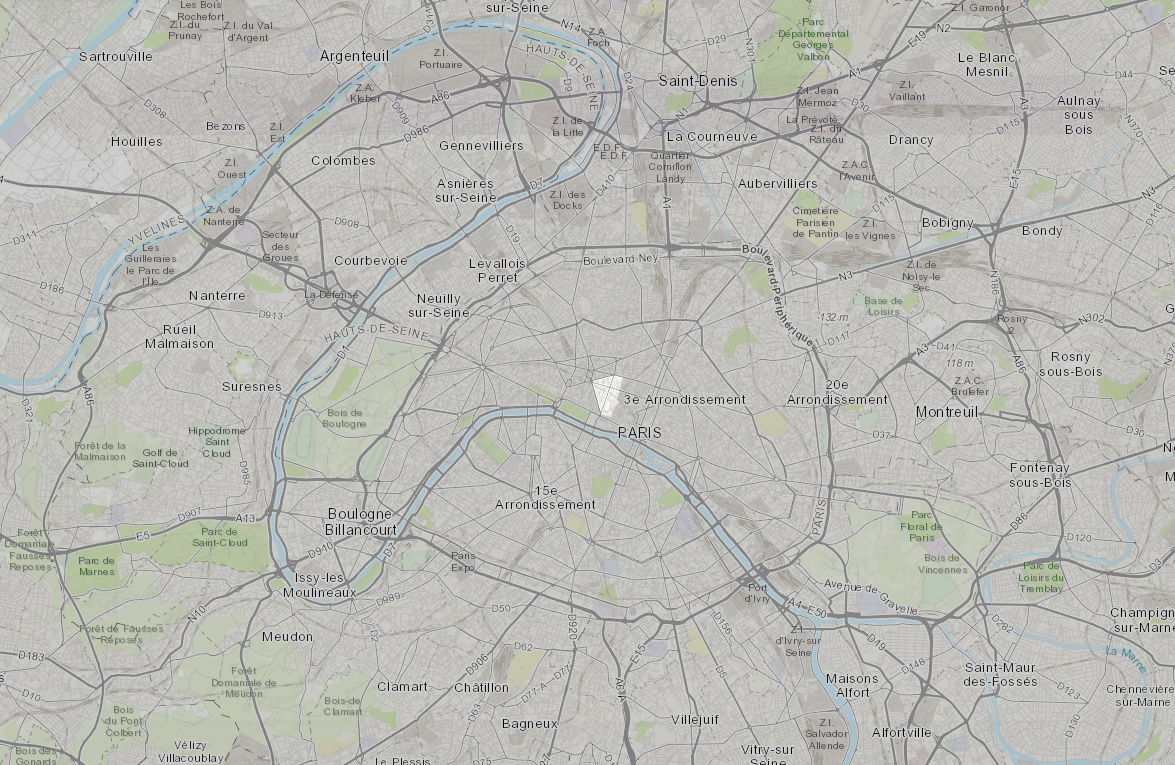
\includegraphics[width=0.7\linewidth]{images/zoom-12.png}
      \caption{Niveau de zoom à 12}
      \label{fig:zoom-12}
    \end{subfigure}
    \begin{subfigure}{.5\textwidth}
      \centering
      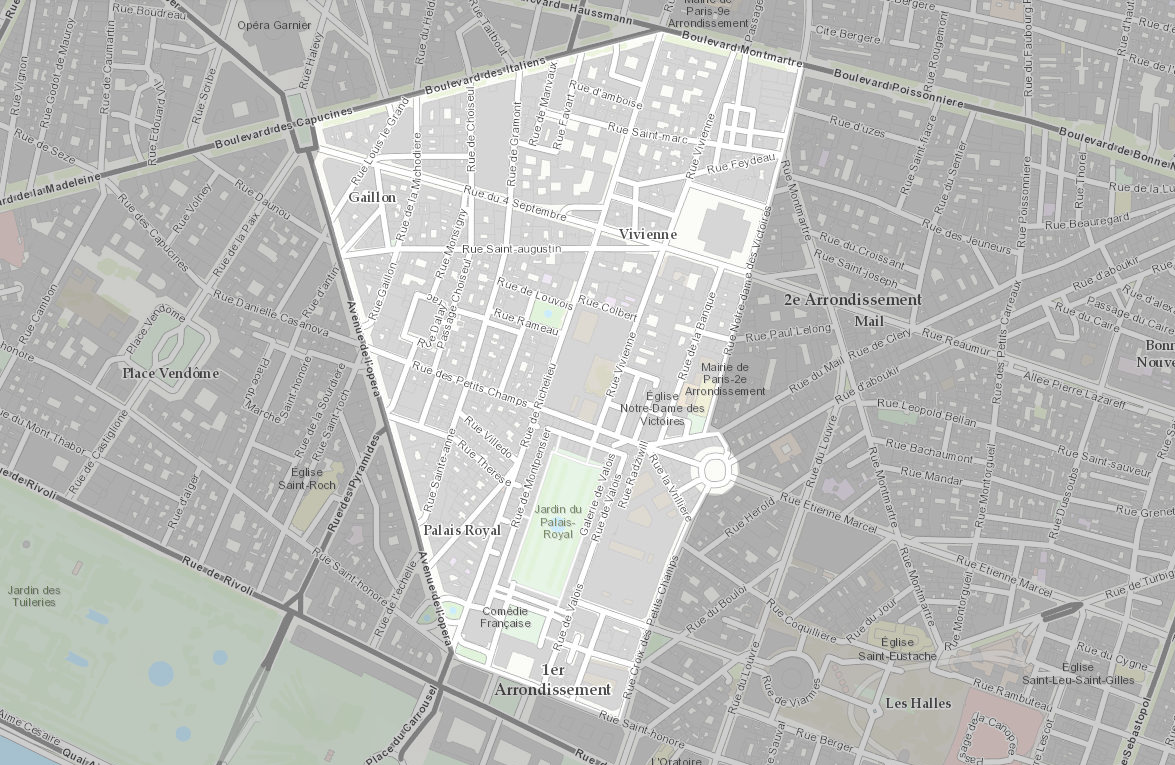
\includegraphics[width=.7\linewidth]{images/zoom-16.png}
      \caption{Niveau de zoom à 16}
      \label{fig:zoom-16}
    \end{subfigure}
\caption{Carte centrée sur Paris puis sur le quartier Richelieu}
\label{fig:zoom}
\end{figure}
Le zoom est un paramètre à ne pas négliger, car il peut influencer le choix du fond de carte. En effet, si le zoom n'est pas correctement limité et que l'utilisateur peut zoomer au maximum, le fond de carte risque de disparaître. Cela s'explique par le fait que les données ne sont pas disponibles à des niveaux de zoom très élevés, car les fonds de carte ont une résolution limitée. Il est donc nécessaire de restreindre les niveaux de zoom afin de gérer ces contraintes techniques.

Notons qu'un autre élément de repère est mis à disposition de l'utilisateur : en plus du zoom qui permet de situer le projet dans Paris, et plus précisément dans le quartier Richelieu, nous avons également délimité une zone spécifique pour le symboliser. Cette zone géographique vient personnaliser la carte en utilisant un objet \acrshort{geojson} qui applique un style spécifique. Il s'agit d'un \texttt{MultiPolygon}, soit une géométrie qui définit plusieurs polygones. Il y a donc un premier polygone qui vient recouvrir une partie de la carte (dont les limites paraissent invisibles car inaccessibles puisque le dézoom est restreint) et un second polygone qui correspond aux limites du quartier Richelieu comme définies par le projet. La première zone est remplie d'une couleur sombre pour donner un effet d'opacité. 

Ainsi, le fond de carte contemporain, le zoom interactif et les délimitations de l'emprise du quartier fournissent des repères spatiaux clairs. Ces premiers éléments ont été conçus pour aider l'utilisateur à interpréter plus facilement la carte et à accéder aux informations historiques tout en les contextualisant géographiquement. Par exemple, le zoom interactif montre que la carte n'est pas statique mais dynamique, incitant l'utilisateur à l'explorer, même avant que les données historiques ne soient affichées. De plus, nous pensons que l'inclusion de repères familiers, tels que les rues et les bâtiments actuels, permet d'établir un lien direct entre le présent et le passé. C'est pourquoi nous proposons d'ajouter un curseur d'opacité entre le fond de carte contemporain et les fonds de cartes historiques.

\subsubsection{Curseur d'opacité avec les fonds de cartes historiques}
Un curseur d'opacité permet de définir la transparence d'un élément, en l'occurrence le degré de visibilité d'un fond de carte.  Cette fonctionnalité ne s'applique pas au fond de carte contemporain, qui est la première couche de la carte, mais aux fonds de cartes historiques. Le curseur permet ainsi de passer du fond de carte contemporain au fond historique sélectionné, le premier servant ainsi de support à la spatialisation d'un phénomène. 
\begin{lstlisting}[language=PYTHON, caption=Variable qui stocke les fonds de cartes historiques en JavaScript]
 var tileLayers = {
      '1. Plan Verniquet (1791)': 'https://tile.ptm.huma-num.fr/tiles/ark/highres/12148/btv1b55013275x/{z}/{x}/{y}.Webp',
      '2. Atlas Vasserot (1810-1836)': 'https://tile.maps.huma-num.fr/uc2usU/d/Alpage_Vasserot_1830/{z}/{x}/{y}.png',
      '3. 1812': 'https://tile.ptm.huma-num.fr/tiles/ark/highres/12148/btv1b530851375/{z}/{x}/{y}.Webp',
      '4. Cadastre municipal (1900)': 'https://tile.maps.huma-num.fr/uc2usU/d/MOSA_1900_PARIS/{z}/{x}/{y}.png',
      '5. 1943': 'https://tile.ptm.huma-num.fr/tiles/ark/highres/12148/btv1b53121232b/{z}/{x}/{y}.Webp', 
    }\end{lstlisting}
    
Cette variable définit un objet JavaScript appelé \texttt{tileLayers} (le pluriel marque la distinction avec la couche initiale \texttt{tileLayer}), qui regroupe les couches de cartes historiques. Chaque entrée représente un fond de carte, identifié par son nom et sa date de création, associés à une \acrshort{url}. Ces \acrshort{url}s pointent vers des données hébergées sur les serveurs de Huma-Num. Certaines cartes ont été générées à l'aide des outils du \acrshort{cstptm}, notamment \acrshort{galligeo}, pour le géoréférencement des cartes de Gallica. Les cartes sélectionnées couvrent la période chronologique du projet. La plus ancienne date de 1791 (plan Verniquet) et la plus récente de 1943 (voir la figure \ref{fig:carto-histo}). Le principal défi dans le choix de ces cartes réside dans leur géoréférencement, qui doit correspondre le plus précisément possible aux données du \acrshort{sig}, sur lesquelles les polygones ont été dessinés. Toutefois, la numérisation des cartes historiques présente dans certains cas des décalages car le papier a été plié et le pli est numérisé, ainsi le polygone est \textit{de facto} décalé (comme en témoigne la figure \ref{fig:verniquet-décalage}). 
\begin{figure}[h!]
    \centering
    \includegraphics[width=0.2\linewidth]{images/décalage-bnf.png}
    \caption{Zoom plan Verniquet (1791), décalage géoréférencement}
    \label{fig:verniquet-décalage}
\end{figure}
Ces cartes sont ensuite ajoutées dans un contrôleur de couches \texttt{layersControl}, une fonctionnalité proposée par Leaflet. Par la suite, chaque carte est gérée via un \textit{slider} \acrshort{html} d'opacité qui permet de modifier directement la transparence de la couche active sélectionnée.
\begin{figure}[h!]
    \centering
    \includegraphics[width=0.5\linewidth]{images/opacité-vasserot-contempo-galerie-vivienne.png}
    \caption{Zoom galerie Vivienne avec faible niveau d'opacité de l'Atlas Vasserot}
    \label{fig:opacité-galerie}
\end{figure}
Cette fonctionnalité offre la possibilité de visualiser les transformations urbaines en superposant plusieurs cartes. Par exemple, la figure \ref{fig:opacité-galerie}  illustre cette utilisation : en haut à droite, le curseur d'opacité est réglé sur une faible valeur, laissant apparaître la carte Vasserot de manière partielle, ce qui permet de la comparer avec la carte contemporaine et de visualiser l'environnement bâti avant la construction de la galerie Vivienne. La figure \ref{fig:opacité-rueVivienne} montre quant à elle la superposition de cartes historiques, entre l'Atlas Vasserot et le cadastre municipal de 1900, pour laisser figurer dans le coin inférieur gauche le percement Nord de la rue Vivienne.
\begin{figure}[h!]
    \centering
    \includegraphics[width=0.5\linewidth]{images/opacité-vasserot-feuille-rue-vivienne.png}
    \caption{Zoom rue Vivienne avec faible niveau d'opacité du cadastre municipal}
    \label{fig:opacité-rueVivienne}
\end{figure} 

Ainsi structuré le code est actif, dynamique et réagit aux ajouts et suppressions de couches que sélectionne l'utilisateur. L'opacité et la visibilité des couches sont ajustées en temps réel sur la carte. Surtout, des informations historiques sont déjà figurées alors qu'aucune connexion à la base de données n'ait  encore effectuée.

% SUBSECTION %%%%%%%%%%%%%%%%%%%%%%%%%
\subsection{Le cartouche : les éléments constitutifs de la carte}
La carte est habillée d'éléments constitutifs, obligatoires dans la cartographie classique, vivement recommandés pour la cartographie Web. Ces éléments sont le titre, la source, la date de création, l'échelle et la légende. D'autres éléments sont facultatifs tels que l'orientation, le cartouche autour de la carte, les toponymes, le quadrillage des coordonnées géographiques (graticule). 
\subsubsection{Le titre, la source et la date}
Le titre, la source et la date sont des éléments qui sont définis par défaut par Leaflet. Il est toutefois possible de modifier les crédits, d'ajouter un hyperlien vers le projet. Les éléments suivants sont facilement modifiables :
\begin{lstlisting}[language=PYTHON, caption=Changement des attributions de la carte en JavaScript]
map.attributionControl.setPrefix('<a href="https://leafletjs.com/">Leaflet</a>');
map.attributionControl.addAttribution('&copy; <a href="https://quartier-richelieu.inha.fr/">Richelieu.Histoire du quartier</a>, Marina Hervieu, 2024');\end{lstlisting}

\subsubsection{L'échelle et l'orientation}
L'échelle et l'orientation sont des éléments issus de plugins. Avec Leaflet, un plugin est une extension qui ajoute des fonctionnalités supplémentaires à la bibliothèque de base. Ils peuvent être développés par la communauté ou par les créateurs de Leaflet, et sont utilisés pour enrichir les cartes interactives avec des options qui ne sont pas incluses dans le cœur de la bibliothèque. Un plugin s’ajoute généralement en important un fichier JavaScript et une feuille de style \acrshort{css} (s'ils sont fournis) dans le projet, puis en initialisant ses fonctionnalités dans le code. 
Voici les plugins (seul le code JavaScript est ajouté) pour l'échelle (\texttt{scale}) et l'orientation (\texttt{compas}):
\begin{lstlisting}[language=PYTHON, caption=Plugins échelle et orientation en JavaScript]
L.control.scale({position:'bottomleft'}).addTo(map);
var compass = L.control.compass({
    position: 'topright',
    autoActive: true  
}).addTo(map); \end{lstlisting}
En complément des lignes de code JavaScript, des modifications sont à apporter dans le code \acrshort{html}, il s'agit de références aux fichiers \acrshort{css} dans le \texttt{<head>} et dans le \texttt{<script>} de JavaScript. Il est à noter que ces fonctionnalités ne sont pas toujours intuitives et que leur implémentation peut entraîner des problèmes de compatibilité. Par exemple, l'orientation a été développée en 2014 avec une version antérieure de Leaflet que celle utilisée acutellement, rendant le plugin initial obsolète. La mise à jour des plugins par la communauté permet cependant de les réutiliser. C'est probablement pour cette raison technique que la plupart des cartes sur le Web ne les intègrent pas, car cela implique de consulter davantage la documentation de Leaflet pour les implémenter correctement.

\subsubsection{Les onglets : la légende et le point \enquote{à propos}}
Enfin, pour faciliter l'ajout d'information sans affaiblir la visibilité de la carte, des onglets comportant la légende et un \enquote{à propos} ont été développés. Il s'agit de panneaux latéraux communément appelés \texttt{sidebar}. 
Au chargement de la carte, un onglet \enquote{à propos} apparaît afin d'expliquer dans les grandes lignes l'objet de la carte et son utilisation. Il se ferme et reste à disposition en haut à gauche, sous le titre de la carte. 
\begin{figure}[h!]
    \centering
    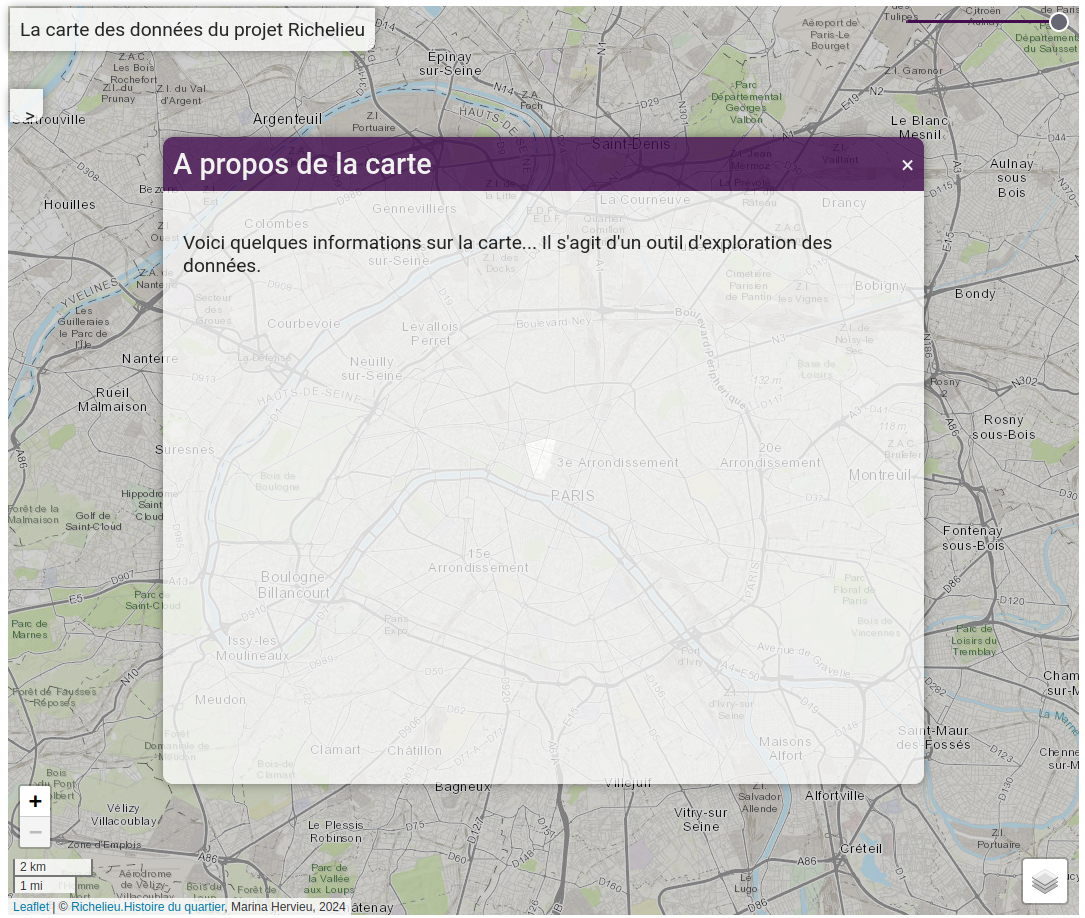
\includegraphics[width=0.75\linewidth]{images/a-propos.png}
    \caption{Onglet \enquote{à propos} au chargement de la carte}
    \label{fig:a-propos}
\end{figure}

L'onglet \enquote{Légende} se trouve quant à lui juste en dessous et enregistre les premiers éléments de légende codés, tels que les couleurs des polygones. Ces onglets sont à considérer comme de nouvelles pages \acrshort{html} que l'on vient ajouter à la carte, la couche initiale. C'est seulement après coup, que nous avons constaté qu'il existe un plugin \texttt{sidebar} développé par Leaflet. A terme, il serait souhaitable de réécrire le code écrit \textit{from scratch} pour l'intégrer via ce plugin certainement plus efficace. 

Pour conclure, les repères contemporains et les éléments structurels sur une carte historique facilitent la compréhension, l'accessibilité, et l'engagement des utilisateurs en leur offrant un cadre spatial connu\footnote{On estime que les utilisateurs de la carte auront \textit{a minima} connaissance de la situation de Paris en tant que capitale de la France} tout en permettant une exploration des données historiques dans un contexte innovant et interactif. Tout l'enjeu de la cartographie Web réside dans ces \enquote{deux fonctions importantes d’une carte : \enquote{susciter des émotions} et \enquote{ancrer dans la réalité}. C’est donc à l’égard de ces deux fonctions que les mondes virtuels peuvent enrichir les représentations cartographiques symboliques. En suscitant des émotions, ils captivent l’attention du lecteur. En ancrant la représentation dans la réalité, ils favorisent la prise de conscience.}\footcite{BUCHERcarte2007}
%%%%%%%%%%%%%%%%%%%%%%%%%%%%%%%%%%%
% SECTION %%%%%%%%%%%%%%%%%%%%%%%%%
\section{Du \textit{back-end} au \textit{front-end}: les requêtes avec l'\acrshort{api}}
Cette section détaille précisément le processus par lequel les données stockées dans la base de données sont requêtées, récupérées et ensuite affichées sur la carte grâce à l'\acrshort{api}, dont le fonctionnement sera présenté. Ce processus est notamment indispensable pour connecter les données à la carte réalisée et présentée dans la précédente section. 
% SUBSECTION %%%%%%%%%%%%%%%%%%%%%%%%%
\subsection{Le fonctionnement d'une \acrshort{api} REST}
\subsubsection{Définition et principes}
Une \acrshort{api}, \textit{Application programming interface} ou interface de programmation d'application permet la communication entre des ressources via une architecture Web de type client-serveur, structurée pour organiser les services en ligne. L'\acrshort{api} repose sur le protocole \acrshort{http} (\textit{HyperText Transfer Protocol}), dont le rôle est de définir les règles de communication entre le client et le serveur\footcite{KERVEGANModelisation2022}. La principale différence entre \acrshort{http} et une \acrshort{api} est que le premier est un protocole générique pour le Web, tandis que l'\acrshort{api} est spécifique à un projet, comme une application, un logiciel ou un ensemble d'applications. Il existe des standards d'interaction entre client et serveur, comme l'\acrshort{api} REST, développée en 2000 par Roy Fielding\footcite{FIELDINFarchitectural2000}. Ce standard est étroitement lié au protocole \acrshort{http}, conçu par le même ingénieur. En somme, l'\acrshort{api} est un code, une "langue" permettant aux machines de communiquer, et elle peut être développée dans des langages tels que Python ou JavaScript.

L'\acrshort{api} REST repose sur plusieurs principes fondamentaux que le projet Richelieu a mis en œuvre. Dans le cadre de cette application, qui utilise PostgreSQL pour le stockage des données, Flask pour la gestion de la logique serveur, et Leaflet pour l'affichage de données cartographiques, l'\acrshort{api} REST organise les interactions entre ces différents composants. Flask expose des routes qui servent de points d'accès aux ressources, permettant d'accéder aux données géospatiales stockées dans PostgreSQL. Chaque route, accessible par des méthodes \acrshort{http} telles que \acrshort{get} ou \acrshort{post}, permet au client (la page \acrshort{html} avec Leaflet) d'effectuer des opérations sur ces données, comme la récupération ou la modification de polygones représentant des zones géographiques, tout en respectant les principes REST. Ces principes incluent une \acrshort{api} sans état  (\textit{stateless}), l'utilisation de méthodes \acrshort{http} standards (\acrshort{get}, \acrshort{post}, PUT, \acrshort{delete}), et l'interaction avec des ressources identifiables via des\acrshort{uri} (\textit{Uniform Resource Identifier}). Chaque requête contient ainsi toutes les informations nécessaires pour être traitée par le serveur, sans maintenir d'état entre les requêtes. Les réponses sont généralement fournies en format \acrshort{json}ou GeoJSON. Plus largement, l'\acrshort{api} REST est devenue très populaire depuis le début des années 2000 (notamment chez Salesforce, Amazon, Google), car elle consomme moins de bande passante, ce qui en fait une solution plus efficace pour les applications en ligne.

\subsubsection{Le requêtage asynchrone}
Le requêtage asynchrone dans ce contexte permet à l'application Web d'envoyer des requêtes à l'\acrshort{api} REST de Flask pour interagir avec les données stockées dans PostgreSQL sans interrompre le fonctionnement de l'interface utilisateur. La requête asynchrone est étroitement liée à l'\acrshort{api} REST dans le sens où elle permet de faire des appels \acrshort{http} à l'\acrshort{api} sans bloquer le fil d'exécution principal de l'application cliente. Une requête asynchrone via JavaScript (par exemple avec \texttt{Fetch API}) permet au client d'envoyer une requête à l'\acrshort{api} REST et d’attendre la réponse tout en continuant à fonctionner. Cela améliore considérablement la réactivité de l'interface utilisateur. Pendant que les données sont récupérées, l'utilisateur peut continuer à interagir avec la page, sans attendre un rechargement complet de celle-ci. Ces deux concepts  interagissent étroitement dans l'application : 
\begin{itemize}
    \item \acrshort{api} REST : La page Leaflet envoie une requête \acrshort{http} (via \acrshort{get} par exemple) à l'\acrshort{api} REST fournie par l'application Flask pour obtenir des données (comme des polygones représentant des lieux).
    \item Requête asynchrone : Cette requête est envoyée de manière asynchrone grâce à Fetch \acrshort{api} en JavaScript, ce qui permet à la page de continuer à fonctionner pendant que les données sont récupérées. 
    \item Réponse \acrshort{json}(ou GeoJSON) : Une fois que Flask a traité la requête et récupéré les données depuis PostgreSQL (en utilisant SQAlchemy dans notre cas), il renvoie les données de nouveau au format \acrshort{json}(ou GeoJSON) à la page \acrshort{html}. 
    \item Affichage des données : Leaflet prend le relais pour afficher les données sur la carte, et tout cela sans aucune interruption visible ou délais de traitement des données pour l'utilisateur de la carte. 
\end{itemize}
Donc l'\acrshort{api} REST fournit des points d'accès (\textit{endpoints}) qui permettent d'interagir avec les ressources (données) sur le serveur, tandis que la requête asynchrone permet d'interagir avec ces points d'accès de façon \enquote{décalée} pour améliorer la fluidité et réactivité de l'application Web. 

% SUBSECTION %%%%%%%%%%%%%%%%%%%%%%%%%
\subsection{Une route de l'application en guise d'exemple}\label{sous-section:fetch-api-places}
Cette route Flask ci-dessous (voir Listing 4.5) expose une \acrshort{api} REST et démontre une requête asynchrone pour récupérer et retourner les données iconographiques d'un lieu en GeoJSON. Détaillons le code pour approfondir la compréhension des principes. 
\begin{lstlisting}[language=PYTHON, caption=Route get-places pour chercher les données iconographiques liées aux lieux et préparer le format de données à envoyer au front-end]
@app.route('/api/places', methods=['GET'])
def get_places():
    # Récupérer tous les lieux
    places = Place.query.all()

    #Variable pour stocker les GeoJSON des lieux
    places_geojson = []

    # Boucle sur chaque lieu
    for place in places:
        # Requête distincte pour récupérer les iconographies associées à ce lieu
        r_iconography_places = R_IconographyPlace.query.filter_by(id_place=place.id).all()
        iconographies = [r.iconography for r in r_iconography_places]
        iconography_count = len(iconographies)  # Compter le nombre d'iconographies pour chaque lieu

        # Utiliser fonction serialize_full 
        iconography_data = [iconography.serialize_full() for iconography in iconographies]

        # Créer la structure GeoJSON pour chaque lieu
        place_data = {
            "type": "Feature",
            "properties": {
                "id": place.id,
                "name": place.id_richelieu,
                "iconography_count": iconography_count,
                "iconographies": iconography_data
            },
            "geometry": place.vector  # La géométrie du lieu en GeoJSON
        }
        places_geojson.append(place_data)

    # Retourner une FeatureCollection sous format GeoJSON
    return jsonify({
        "type": "FeatureCollection",
        "features": places_geojson
    })\end{lstlisting}
L'\acrshort{api} REST est exposée via la route \texttt{@app.route('/api/places', methods=['GET'])} dont \texttt{'/api/places'} est le point d'accès. Elle permet à l'application cliente d'envoyer des requêtes \acrshort{http} \acrshort{get} à l'\acrshort{api} pour récupérer les informations sur les lieux et leurs iconographies associées. Les données sont clairement exposées sous forme de ressources, et chaque lieu est une ressource représentée par un GeoJSON que le client demande. En effet, celui-ci envoie une requête asynchrone via la fonction JavaScript \texttt{fetch()} pour récupérer les données. Les données stockées sont traitées via une requête \acrshort{sql} et un formatage. Le serveur Flask interroge la base de données PostgreSQL via SQLAlchemy pour récupérer les lieux (\texttt{Place.query.all()}) et, pour chaque lieu, il récupère les iconographies associées via la table de relation \texttt{R\_IconographyPlace}. Pour chaque lieu, les données sont organisées dans une structure GeoJSON, qui comprend les informations géométriques (via \texttt{place.vector}) ainsi que les propriétés du lieu, comme son ID, son nom, et les iconographies associées via \texttt{serialize\_full} (une fonction prédéfinie pour récupérer toutes les informations telles que les métadonnées des iconographies) ainsi qu'un compte du nombre d'iconographies par lieu. L'ensemble de ces informations sont ensuite retournées par le serveur dans une \texttt{FeatureCollection} GeoJSON, un format adapté à des bibliothèques comme Leaflet pour afficher des données géospatiales sur une carte. La réponse est encapsulée dans un format \acrshort{json}via \texttt{jsonify()}, respectant les standards de l'\acrshort{api} REST. 

Cette route est un exemple parmi d'autres codes développés pour interagir avec les données à préparer pour la carte. La prochaine étape du développement de l'outil consiste à tester la requête pour s'assurer que les données GeoJSON sont correctement récupérées d'une part, et correctement affichées sur la carte d'autre part. 
%%%%%%%%%%%%%%%%%%%%%%%%%%%%%%%%%%%
% SECTION %%%%%%%%%%%%%%%%%%%%%%%%%
\section{L'affichage des données}
L'affichage des données relève du \textit{front-end} de l'application. Cette section présentera quelques exemples de visualisation des données ainsi quelques éléments du code développé pour les réaliser. 
% SUBSECTION %%%%%%%%%%%%%%%%%%%%%%%%%
\subsection{Le lieu figuré par les parcelles}
Le lieu, en tant qu'entité principale du modèle de données du projet Richelieu, est représenté par un ensemble de géométries définies par des coordonnées géographiques. Ces géométries peuvent prendre la forme de polygones, qui représentent une surface fermée définie par plusieurs paires de coordonnées, la première et la dernière devant être identiques pour former un polygone fermé. Dans d'autres cas, lorsque les lieux représentent une rue ou un point d'intérêt, ils sont définis par un point unique avec une seule paire de coordonnées. Ensemble, ces éléments constituent les parcelles à positionner sur la carte, à partir desquelles l'exploration des données s'effectue.

\subsubsection{De l'affichage par défaut à la personnalisation}
Leaflet utilise de nombreux paramètres par défaut pour afficher les données, notamment dans le cas des lieux. Cependant, il est nécessaire de spécifier dans le formatage des données le type de géométrie : les polygones sont des \texttt{vector}, tandis que les points sont des \texttt{centroid}, sachant que chaque polygone possède également un point central, calculé automatiquement par défaut - ci-dessous un extrait de données au format GeoJSON.  

\begin{lstlisting}[language=PYTHON, caption=Structure GeoJSON]
{
   "type": "FeatureCollection",
   "features": [
       {
          "type": "Feature",
          "geometry": {
            "type": "Point",
            "coordinates": [  
                2.339712423376673,
                48.86822533019579
                ],
          },
          "properties": {
            "title": "Rue Vivienne"
          }
        },
        {
          "type": "Feature",
          "geometry": {
            "type": "Polygon",
            "coordinates": [
              [
                [
                  2.337516076011978,
                  48.86677742624936
                ],
                [
                  2.3382407144394213,
                  48.868162909802265
                ],
                [
                  ...
                ],
                [
                  2.337516076011978,
                  48.86677742624936
                ]
              ]
            ],
          },
          "properties": {
            "title": "2 Rue Vivienne"
          }
        }
    ]
}
\end{lstlisting}
À partir de ce fichier reçu par le client, celui-ci propose un affichage par défaut: il expose la donnée via des points (voir la figure \ref{fig:2eme-affichage}) plutôt que par des polygones, il convient de lui préciser le formatage des données attendu afin de l'afficher comme illustré (voir figure \ref{fig:1er-affichage}), par exemple. 

\begin{figure}[h!]
    \begin{subfigure}{.5\textwidth}
      \centering
    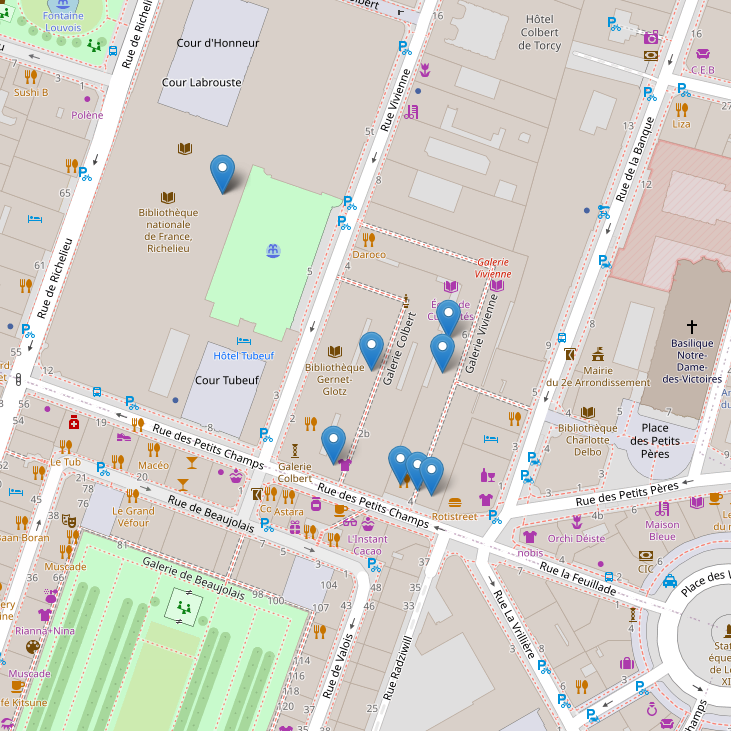
\includegraphics[width=.7\linewidth]{images/1er-affichage.png}
    \caption{Sans formatage précisé}
    \label{fig:2eme-affichage}
    \end{subfigure}
    \begin{subfigure}{.5\textwidth}
      \centering
      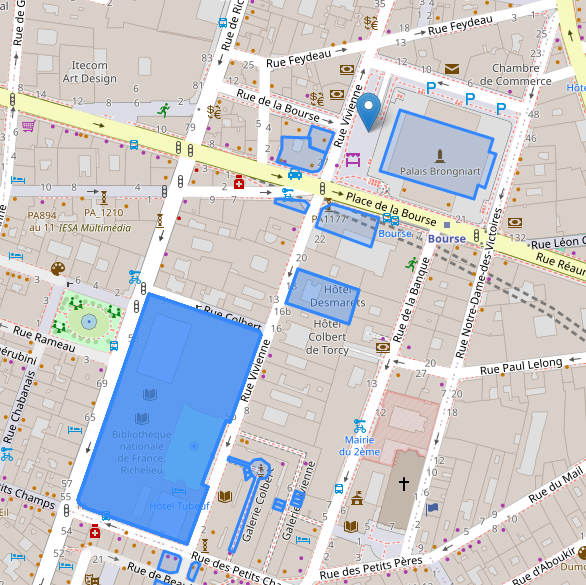
\includegraphics[width=0.7\linewidth]{images/2eme-affichage.png}
    \caption{Avec formatage précisé}
    \label{fig:1er-affichage}
    \end{subfigure}
    \caption{Exemple d'affichage sans et avec formatage précisé des données de lieux}
\label{fig:affichage-defauts}
\end{figure}

\subsubsection{La fonction \texttt{fetch}}
Pour ce faire, on utilise la fonction \texttt{fetch} en JavaScript car elle permet d'effectuer des requêtes \acrshort{http} asynchrones vers un serveur, pour récupérer des données, généralement au format JSON, ou envoyer des données. Elle est très souvent utilisée pour obtenir et traiter des informations sans avoir à recharger la page, comme dans l'exemple où le client, l'application, doit récupérer des polygones ou des points. \texttt{fetch} prend comme premier paramètre l'\acrshort{url} de la ressource à récupérer, et retourne la réponse. Une fois la réponse reçue, il est possible de l'exploiter, par exemple en la convertissant en GeoJSON pour un traitement ultérieur. 
\begin{lstlisting}[language=HTML, caption=Exemple d'utilisation de la fonction fetch]
fetch('/api/places')
  .then(response => response.json()) 
  .then(data => {
    L.geoJSON(data).addTo(map); 
  })
  .catch(error => console.error('Erreur lors de la récupération des données:', error));
\end{lstlisting}

La requête \texttt{fetch('/api/places')} envoie une requête \acrshort{get} à l'\acrshort{api} REST, elle demande à avoir les données sur les lieux exposées par Flask. La réponse est ici convertie en \acrshort{json}avec \texttt{response.json()} et les données récupérées sont ajoutées à la carte Leaflet via la ligne \texttt{L.geoJSON(data).addTo(map);}. Au même titre que la fonction \texttt{print()} en Python, le \texttt{console.log} est une technique constamment utilisée pour afficher des informations, un message ou des repères sur la console du navigateur Web (accessible par \texttt{ctrl + i}.

\subsubsection{Le type de données}
Il est cependant important de bien interpréter la nature des données récupérées, car celles-ci correspondent à des représentations géographiques spécifiques. Dans la mesure où la donnée du lieu est représentée par des parcelles géographiques, il convient de préciser qu'elles correspondent à un type particulier de donnée. Les polygones sont des données qualitatives nominales zonales, c'est-à-dire des surfaces délimitées, comme nous l'avons défini au cours du chapitre précédent avec le choix porté sur une carte choroplèthe (voir chapitre \ref{section:choix-carto}). En revanche, lorsque les lieux sont représentés par des points, ils relèvent de données qualitatives ponctuelles. Les données qualitatives nominales sont un type de données qualitatives (ou catégoriques) qui servent à classer ou identifier des éléments en fonction de catégories ou de labels, sans ordre particulier. Elles sont non numériques et ne possèdent aucune hiérarchie ou relation d'ordre entre les catégories. Chaque catégorie est unique même si les lieux peuvent être classés par type (parcelle, aile, ensemble, rue, etc.). L'objectif est simplement de distinguer les différents éléments ou groupes, sans qu'il y ait une notion de quantité ou d'intensité. Par exemple, les couleurs (rouge, vert, bleu) sont différentes et ne représentent aucun ordre. Ainsi les polygones n'ont pas de relation d'ordre entre eux, mais il est toutefois possible de classer visuellement les zones sur la carte, nous verrons en détail ce point par la suite. Surtout, ces distinctions sont essentielles pour interpréter correctement la nature des données géographiques et leur représentation visuelle sur la carte. 

% SUBSECTION %%%%%%%%%%%%%%%%%%%%%%%%%
\subsection{Mettre en scène les données}
Une fois que la communication des données entre le \textit{front-end} et le \textit{back-end } est mise en place dans l'application et assimilée par le développeur, il convient de les mettre en scène en exploitant autant que possible les langages du Web (\acrshort{html}, \acrshort{css} et JavaScript).
\subsubsection{Une question de d'échelle : les niveaux de granularité}
Nous avons vu lors du chapitre sur la modélisation de la donnée (voir \ref{sous-section:modele-bddr}) que les sources cartographiques sont réparties par niveaux de granularité. Nous avons ainsi tenté de proposer une première exploration des données à travers ce paramètre.
\begin{lstlisting}[language=PYTHON, caption=Récupérer les données cartographiques par granularité]
@app.route('/i/fetch-carto/', methods=['GET'])
def fetch_carto():
    '''
    fetch données cartographiques et retourner dans un GeoJSON Feature Collection 
    '''
    #méthode .split() utilisée pour séparer les arguments requêtés par le front
    
    carto = request.args.get('carto', '').split(' ')
    granularity = request.args.get('granularity', '').split(' ')
    print('%%', carto, granularity)
    r = db.session.execute(text("SELECT * FROM cartography;"))
    print(r.all())

 
    def feature_factory(cartography) -> dict:
        '''
        obtenir un objet cartographique et le retourner 
        '''
        return { "type":"Feature",
                 "geometry":cartography.vector,
                 "properties": { "id_uuid": cartography.id_uuid,
                                  "map_source": cartography.map_source,
                                  "granularity" : cartography.granularity                                  
                                  } } 
                                  
    #requête avec liste compréhensive
    #* décompose la liste compréhension en arguments
    #and_ garantit que les deux conditions sont vraies pour cartography.granularity&cartography.map_source
    #pour chaque combinaison, générer une condition de filtrage
    r = db.session.query(Cartography).filter(
        or_(*[
            and_(Cartography.granularity == grain, Cartography.map_source == cart)
                for grain in granularity  
                for cart in carto  
            ])
        )
    features = [ feature_factory(cartography) for cartography in r.all() ]
    print('%%%%%%%%%%', r)
    feature_collection = { "type": "FeatureCollection", "features": features }

    return jsonify(feature_collection)
\end{lstlisting}

\sloppy La fonction \texttt{fetch\_carto()} est accessible via l'\acrshort{url} \texttt{/i/fetch-carto/} qui utilise la méthode \acrshort{http} \acrshort{get}. Elle récupère des objets cartographiques filtrés par \texttt{carto} et \texttt{granularity} depuis la base de données. Les arguments passés dans l'\acrshort{url} (par exemple, \texttt{/i/fetch-carto/?carto=example\&granularity=detail)} sont récupérés par \texttt{request.args.get()}. Les arguments \texttt{carto} et \texttt{granularity} sont séparés en listes à l'aide de la méthode \texttt{.split(' ')}. Cela permet de traiter plusieurs valeurs passées dans l'\acrshort{url} en une seule chaîne de caractères, séparées par des espaces : \texttt{carto = ['exemple1', 'exemple2']} et \texttt{granularity = ['ensemble', 'aile']}. Puis la fonction \texttt{feature\_factory()} prend en argument un objet cartographique et le formate en GeoJSON. Elle renvoie ainsi le dictionnaire (\enquote{clé:valeur}) contenant le type de géométrie de l'objet, la géométrie en question et ses propriétés comme la granularité. 

Ensuite, une requête avec SQLAlchemy filtre les données en fonction des arguments passés dans l'\acrshort{url}. La condition \texttt{or\_(*[...])} recherche toutes les combinaisons possibles entre \texttt{carto} et \texttt{granularity} - un premier développement a essayé de résoudre ce point manuellement mais il s'est avéré incomplet. Cette condition assure que les deux conditions (granularity et map\_source) soient remplies pour chaque combinaison. La boucle imbriquée permet de générer les combinaisons et d'appliquer ces conditions de filtrage.

Nous estimons que ce paramètre permet de comprendre les différentes échelles de représentation figurées dans les sources qui reflètent la réalité bâtie. Une première visualisation offre à l'utilisateur la possibilité de sélectionner la granularité souhaitée, comme en témoigne les figures \ref{fig:gran-parcelle} et \ref{fig:gran-galerie}.  Il convient de noter que cet exemple repose sur une version préliminaire de la base de données, qui ne reflète pas encore le corpus final des données ; par exemple, la Banque de France n'y est pas encore incluse. 
\begin{figure}[h!]
    \begin{subfigure}{.5\textwidth}
      \centering
    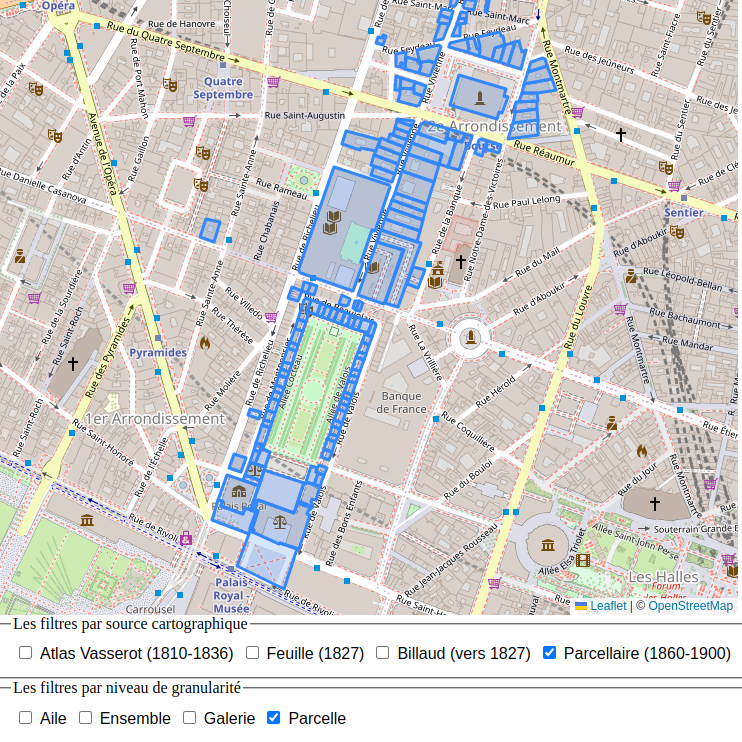
\includegraphics[width=.7\linewidth]{images/gran-parcelle.png}
    \caption{Affichage par parcelle}
    \label{fig:gran-parcelle}
    \end{subfigure}
    \begin{subfigure}{.5\textwidth}
      \centering
      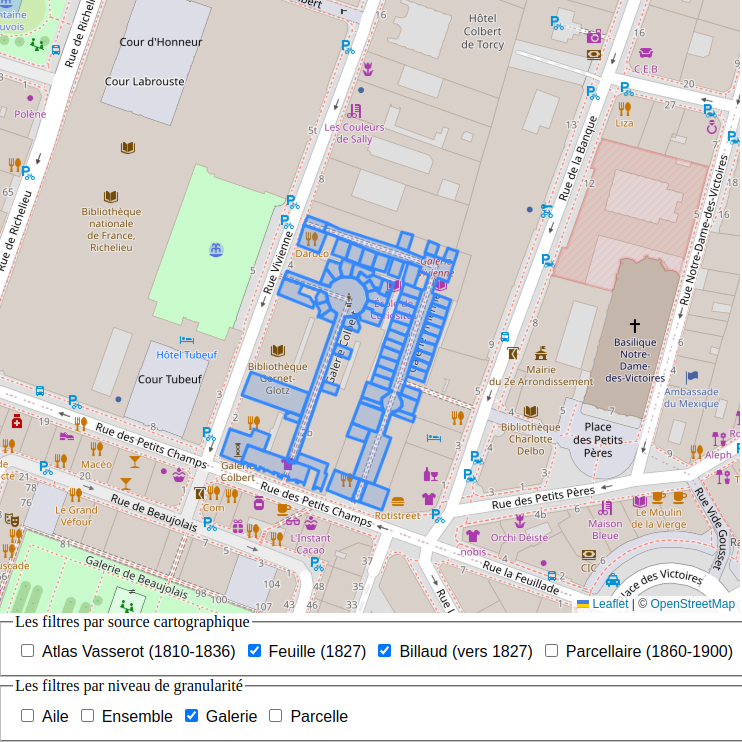
\includegraphics[width=0.7\linewidth]{images/gran-galerie.png}
    \caption{Affichage par galerie}
    \label{fig:gran-galerie}
    \end{subfigure}
    \caption{Exemple d'affichage sans et avec formatage précisé des données de lieux}
\label{fig:granularité}
\end{figure}

Le code est ainsi récupéré par une fonction \texttt{fetch()} qui prend en arguments \texttt{data} et \texttt{category}, représentant respectivement la donnée et la catégorie associée. Ces variables sont ensuite liées à un élément \acrshort{html} \texttt{checkbox}, un ensemble de cases à cocher, dont chaque catégorie possède son identifiant. Une fonction JavaScript est ensuite déclenchée pour afficher les données en fonction de la \texttt{box} cochée.

Cependant, nous avons rapidement constaté que cette approche présente certains inconvénients, comme illustré par la figure \ref{fig:gran-tout}. L'interprétation des données devient complexe. En effet, lorsque tous les paramètres sont sélectionnés, les données s'agrègent, mais les polygones issus des différentes sources cartographiques se superposent, révélant un décalage significatif. Que peut signifier ce phénomène ? Il semble que ces écarts reflètent les divergences entre les sources historiques et les variations dans les niveaux de détail ou de granularité. Il y a donc un polygone par source cartographique et par niveau de granularité, et ces polygones ne correspondent pas toujours parfaitement. Cela est probablement dû à l'utilisation de projections cartographiques différentes lors du géoréférencement des polygones dans le \acrshort{sig}.

\begin{figure}[h!]
    \centering
    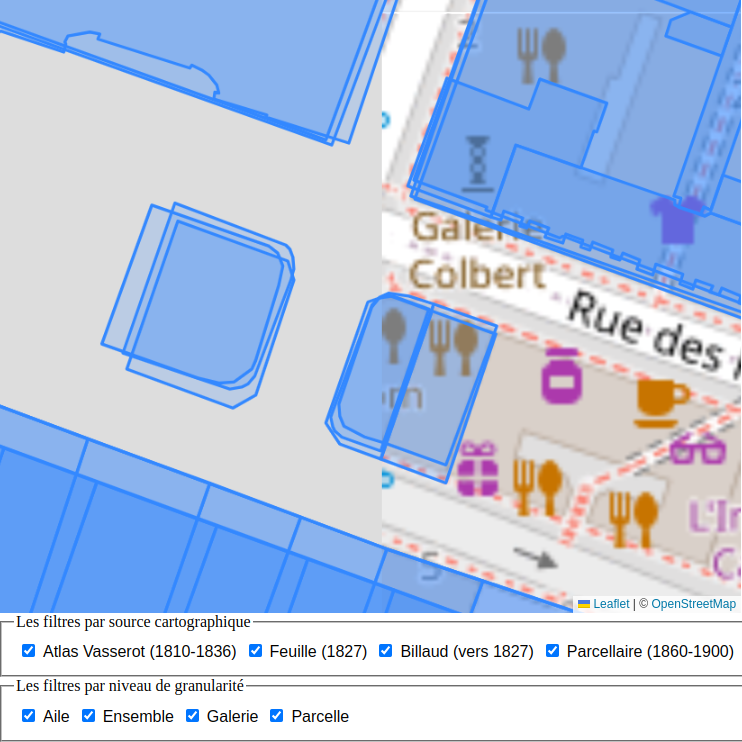
\includegraphics[width=0.4\linewidth]{images/gran-tout.png}
    \caption{Toutes les granularités sélectionnées}
    \label{fig:gran-tout}
\end{figure}

Finalement, requêter à partir de la table \texttt{Place} est la solution la plus adéquate car elle fournit une structure complète, unique et cohérente du lieu comme entité géographique et elle centralise toutes les informations liées. 

\subsubsection{Une figuration de la densité d'information : \textit{heatmap} parcellaire}
Pour se concentrer sur la notion de lieu, nous proposons de représenter la densité d'informations iconographiques liées à chaque lieu. Il s'agit d'une \textit{heatmap} parcellaire ou carte de chaleur, où la \enquote{chaleur} est représentée par la couleur de chaque parcelle ou zone sur la carte, en fonction du nombre de sources iconographiques associées. Cette proposition s'apparente donc à une carte choroplèthe zonale.

\begin{figure}[h!]
    \centering
    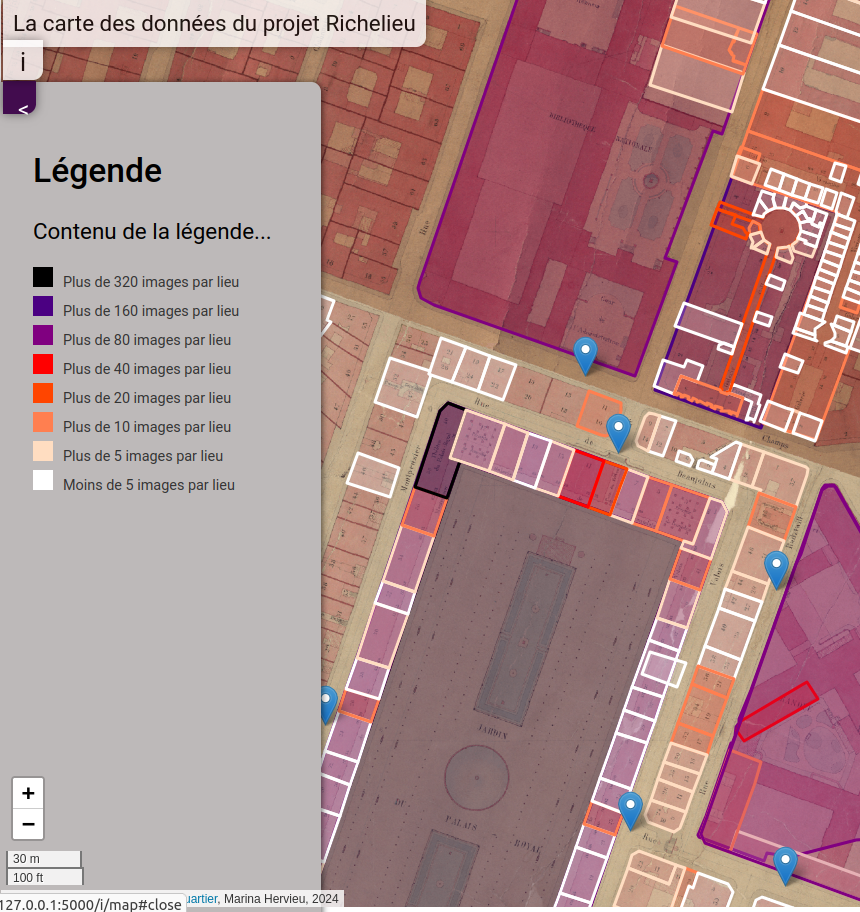
\includegraphics[width=0.75\linewidth]{images/heat-map-density.png}
    \caption{\textit{Heatmap} parcellaire pour la densité d'informations iconographiques, accompagnée de sa légende}
    \label{fig:heat-map}
\end{figure}

Le code en question utilise la fonction \texttt{fetch('/api/places')} présentée dans la section \ref{sous-section:fetch-api-places} pour récupérer les données GeoJSON des lieux à partir de l'\acrshort{api}. Cette requête a la particularité de comptabiliser le nombre d'iconographies par lieu. Une fois ces données obtenues, elles sont stylisées en fonction de la densité d'informations présentes pour chaque lieu. Chaque polygone (représentant une parcelle) est coloré en fonction du nombre d'iconographies associées, grâce à la fonction \texttt{getColorForCount(count)}. Par exemple, une parcelle avec plus de 320 iconographies sera colorée en noir, tandis qu'une autre avec moins de 5 iconographies sera blanche. Comme l'indique le tableau ci-suit(\ref{tab:legende}), beaucoup  de lieux possèdent entre 1 et 5 iconographies, avec une décroissance rapide au~-~delà. Pour définir les seuils de couleurs dans la légende, nous avons utilisé une fonction exponentielle de la forme $5 \times 2^n$. Cette approche permet de visualiser rapidement la concentration des sources iconographiques dans certaines zones : plus la couleur est foncée, plus la densité de sources est élevée.

\begin{table}[!]
    \centering
    \begin{tabular}{|l|c|}
    \toprule
        \textbf{Nombre d'iconographies} & \textbf{Nombre de lieux}\\
    \midrule
         5  & 149 \\
         10 & 60 \\
         20 & 43 \\
         40 & 17 \\
         80 & 13 \\
         160 & 9 \\
         320 & 6 \\
         < 320 & 2 \\
        \bottomrule
    \end{tabular}
    \caption{Calcul du nombre de lieux par nombre d'iconographies}
    \label{tab:legende}
\end{table}
 
La carte permet ainsi de visualiser la répartition inégale des sources cartographiques et iconographiques par lieu - pour des raisons que nous avons déjà expliquées (voir \ref{sous-section:lieu}). En effet, une première analyse de la répartition des sources (figurée dans un camembert ou d'autres graphiques) montre que la majorité des sources est concentrée sur un petit nombre de lieux. Cela correspond également à l'affichage sur la carte, où certaines parcelles apparaissent plus denses en informations, tandis que la majorité des lieux possède beaucoup moins de données. On remarque aisément en noir le \enquote{RM 19}, soit le 19, rue Montpensier (voir le paragraphe correspond \ref{sous-sous-section:rm19}). Cette carte de chaleur met donc en lumière une distribution déséquilibrée des sources, avec une forte concentration d'iconographies et de documents sur quelques lieux emblématiques. 


\subsubsection{Les images liées}
Enfin, il convient de faire apparaître par lieu les iconographies qui y sont liées. Elles sont visualisées sur la carte de façon interactive. 

\begin{figure}[h!]
    \begin{subfigure}{.5\textwidth}
      \centering
    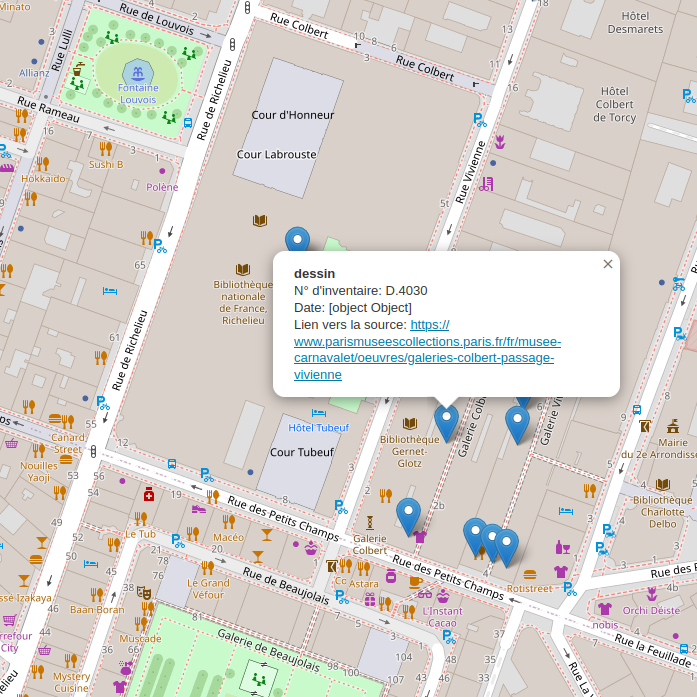
\includegraphics[width=.7\linewidth]{images/pop-up-old.png}
    \caption{Pop-up essai n°1 }
    \label{fig:pop-up-old}
    \end{subfigure}
    \begin{subfigure}{.5\textwidth}
      \centering
    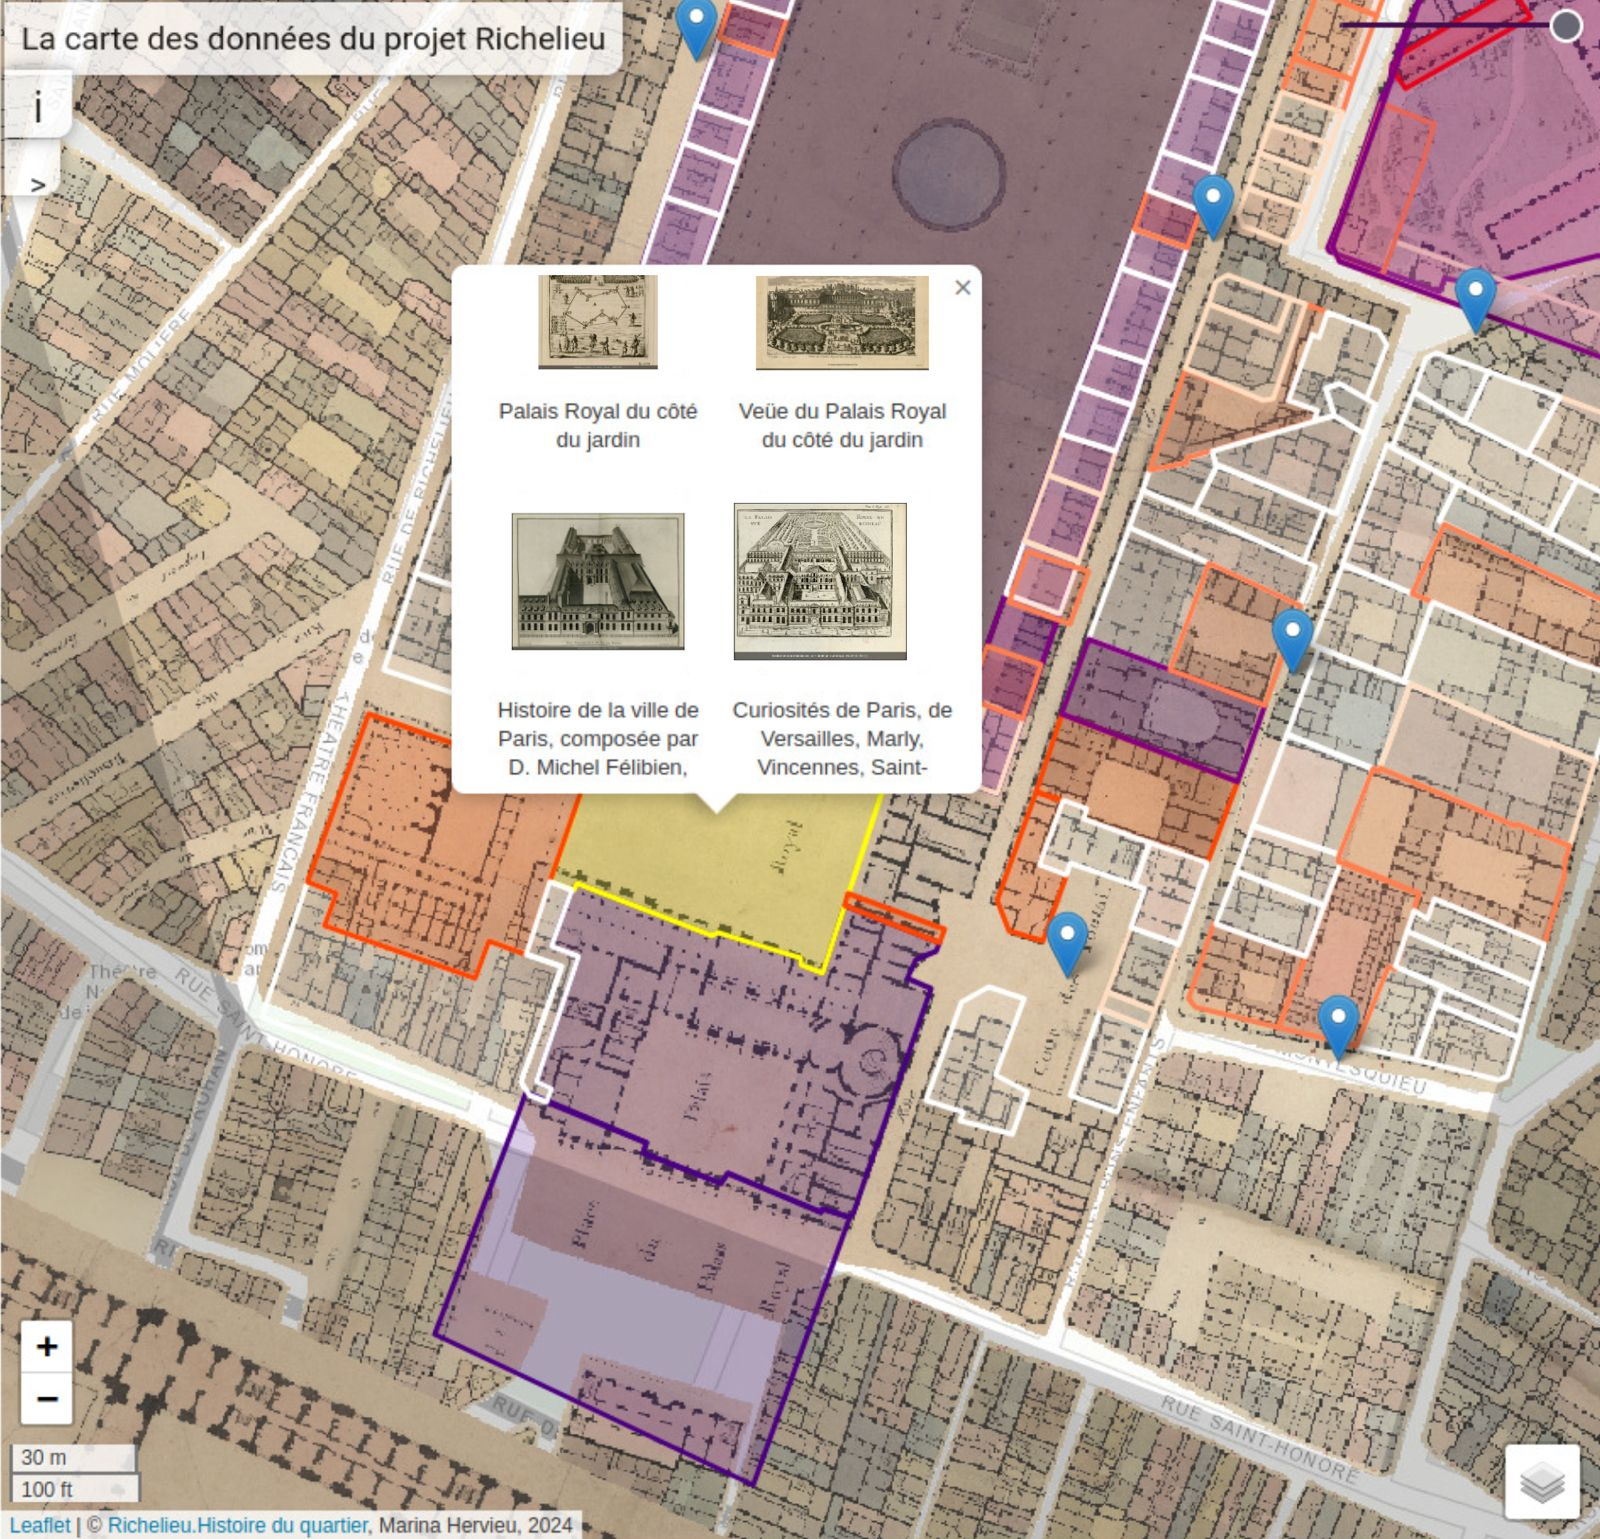
\includegraphics[width=.7\linewidth]{images/pop-up.jpeg}
    \caption{Pop-up essai n°2}
    \label{fig:pop-up}
    \end{subfigure}
    \caption{Exemple d'affichage des iconographies liées aux lieux}
\label{fig:pop-up-all}
\end{figure}

Lorsqu'un utilisateur clique sur un des points dans la figure \ref{fig:pop-up-old} ou sur une des parcelles comme dans la figure \ref{fig:pop-up}, un pop-up s'ouvre pour afficher des informations détaillées (le titre, l'auteur, la date de création, le numéro d'inventaire, etc.) sur le lieu ainsi que les iconographies associées. Le code ci-dessous permet d'afficher une galerie d'images directement dans le pop-up, avec les données récupérées pour chaque lieu. Chaque image dans la galerie est liée à une source iconographique via une \acrshort{url} \acrshort{iiif}. Si l'utilisateur rencontre un problème pour afficher en miniature les images \acrshort{iiif}, il peut cliquer sur l'encart qui devrait accueillir l'image, alors elle s'ouvre dans un nouvel onglet. Cet effet n'est pas un paramètre par défaut de Leaflet et correspond à l'élément \acrshort{html} \texttt{alt} dans le code ci-dessous. Si plusieurs titres sont associés à une image, alors une galerie d'images est générée et elles sont combinées et affichées en deux colonnes, permettant à l'utilisateur d'explorer visuellement les ressources liées à ce lieu sans entraver l'exploration sur le reste de la carte. De plus, le polygone change de couleur quand il a déjà été visité (il devient jaune). Ce mécanisme est illustré dans le figure \ref{fig:pop-up}. Il permet à l'utilisateur de se situer sur la carte. 

\begin{lstlisting}[language=HTML, caption=Création d'un pop-up et d'une galerie d'images]
function showImageGalerie(placeId, layer, iconographies) {
    if (iconographies && iconographies.length > 0) {
        var galerieHtml = '<div class="popup-galerie">';
        iconographies.forEach(function(iconography) {
            var sourceUrl = iconography.source_url || '';  /
            var title = iconography.title ? iconography.title.join(', ') : 'Untitled';  
            galerieHtml += '<div class="popup-galerie-item">';
            galerieHtml += '<img src="' + sourceUrl + '" class="popup-galerie-image" alt="' + title + '"/>';  
            galerieHtml += '<p>' + title + '</p>';  
            galerieHtml += '</div>';
            });
        galerieHtml += '</div>';
        layer.bindPopup(galerieHtml, { maxHeight: 300 }).openPopup();
        } else {
        layer.bindPopup('<p>Il n'y a pas d'images liées à ce lieu.</p>').openPopup();
        }
    }
\end{lstlisting}
Ce code JavaScript définit la fonction \texttt{showImageGalerie}. Un conteneur \acrshort{html} est créée pour contenir la galerie d'images. Ce conteneur est initialisé avec une \texttt{div} de la classe \texttt{popup-galerie}. Puis une boucle \texttt{iconographies.forEach} parcourt chaque iconographie associée au lieu cliqué pour créer un élément \acrshort{html} pour chacune des iconographies. Enfin une variable vient récupérer et stocker l'\acrshort{url} de l'image et la variable \texttt{title} récupère le titre. Puis, un élément \acrshort{html} est généré pour chaque item de la galerie dont l'\texttt{img src} (\acrshort{url} pointant vers la source de l'image) et un texte alternatif, défini par l'attribut \texttt{alt}, s'affiche lorsque l'image ne peut pas être chargée. Puis la galerie d'images est fermée avec la \texttt{</div>}.
Pour afficher la galerie dans un pop-up, un cartel interactif, on utilise une fonctionnalité de Leaflet \texttt{bindPopup} qu'on associe au contenu \acrshort{html} \texttt{galerieHTML} généré juste avant. Un message informationnel est aussi ajouté en cas d'absence d'image liée au lieu. A travers ce code, on propose de créer automatiquement les éléments \acrshort{html} via le JavaScript. 

Finalement, ce système de visualisation dynamique permet une exploration intuitive des lieux en relation avec leurs iconographies historiques, renforçant ainsi l'engagement avec les données géographiques et patrimoniales. 

\subsubsection{Des initiatives à l'état de brouillon}
Les développements mentionnés précédemment ne représentent que quelques exemples parmi d'autres initiatives. Un \textit{slider} temporel a notamment été implémenté pour afficher les parcelles correspondant aux images associées à la date sélectionnée. Toutefois, le résultat final s'est révélé peu satisfaisant , car les données ont effectivement été écrasées (comme anticipé au chapitre \ref{sous-sous-section:chrono}), et le manque de temps a constitué une contrainte pour résoudre ce problème.Ainsi il semble en effet complexe de combiner de manière fluide l'ensemble des axes de recherche – temps, espace et iconographie – sur une seule carte. Une approche alternative pourrait consister à proposer des mini-cartes encapsulées dans la carte principale, offrant ainsi une visualisation plus spécifique et ciblée\footnote{La carte Artl@s est disponible \href{https://paris-art-market.huma-num.fr/}{ici} opte pour cette solution par exemple.}. Il y aurait une carte principale qui propose en option, une carte visualisant la granularité des données; puis une carte visualisant la densité des données. Par ailleurs, le développement de filtres thématiques, ainsi que la fonctionnalité de sélection et de sauvegarde de zones, n'a pas pu être mené à terme. Toutefois, selon le \acrshort{mvp}, les fonctionnalités en orange ont toutes été développées. 

\subsubsection{Conclusion du chapitre}
Pour conclure, nous avons vu que la réalisation technique de la carte s'inscrit dans un processus de développement  \textit{full-stack} en plusieurs étapes, débutant par la définition des fonctionnalités structurelles via la bibliothèque Leaflet, comme le fond de carte, le cartouche et les éléments interactifs. La connexion à la base de données a ensuite été établie grâce à une \acrshort{api} REST, permettant de récupérer et d'afficher dynamiquement les données sur la carte, offrant une exploration interactive des lieux et des iconographies du projet Richelieu. L'intégration des fonds de carte et des couches superposées a permis une gestion en temps réel de la visibilité des informations, tandis que la connexion à la base de données a enrichi la carte avec des données dynamiques. Le rôle central de l'\acrshort{api} REST a facilité l'échange de ces données, démontrant ainsi la flexibilité et l'efficacité de cette architecture pour offrir des visualisations variées, tout en maintenant la connexion avec les sources historiques. Ce chapitre souligne l'importance de la cartographie Web interactive pour rendre les données historiques plus accessibles, tout en les ancrant dans la réalité du projet.

\subsubsection{Conclusion de la deuxième partie}
Dans cette deuxième partie, les différentes étapes de la conception et du développement de la carte Web en tant qu'outil d'exploration des données ont été exposées. Grâce à une approche méthodique, nous avons défini les objectifs de visualisation des données en lien avec le projet Richelieu, tout en prenant en compte les contraintes techniques et les attentes fonctionnelles. La visualisation des données du projet Richelieu s'effectue à travers une carte choroplèthe, offrant diverses possibilités pour varier l'affichage selon la densité ou la granularité. Cependant, elle ne peut intégrer la dimension de réseau, bien que cela ait été souhaité au départ du projet. De plus, la représentation précise de la dimension temporelle reste complexe et limitée en moyen tant humain que temporel.

La carte présente néanmoins un avantage majeur, en ligne avec la vision de Malraux et de son musée imaginaire\footcite{MALRAUXMusee1996} : dans un espace restreint, à l'échelle d'un quartier, elle réunit un nombre considérable de sources iconographiques et cartographiques provenant de diverses institutions, y compris étrangères. Toutefois, la carte ne peut offrir une visualisation exhaustive : elle n'affiche pas toutes les informations associées à une image. Or, l'histoire de l'art étant une discipline rigoureuse, il est essentiel de mentionner les sources, les techniques, la datation et d'autres informations qui ne peuvent être pleinement lues sur la carte à défaut de la rendre illisible. Cependant, la cartographie sur le Web permet d'accéder, d'un simple clic, à l'ensemble de ces données complémentaires grâce à un renvoi vers la page principale de l'image qui détaille ces informations sur le site du projet Richelieu.

Quant à savoir si la carte est avant tout une \textit{démonstration} ou un objet de \textit{recherche}, ou peut-être les deux, comme le suggère Grandjean, il revient aux utilisateurs, d'une part, et, aux chercheurs d'autre part,  d'explorer cet outil pour déterminer s'il offre de nouvelles perspectives de recherche sur le quartier Richelieu.

%%%%%%%%%%%%%% PART 3 %%%%%%%%%%%%%%%%%%%%%%%%%%%%%%%%%%%
%%%%%%%%%%%%%%%%%%%%%%%%%%%%%%%%%%%%%%%%%%%%%%%%%%%%%%%%%
\part{Perspectives en réflexion : intégration, pérennité et enjeux futurs du projet}
Cette troisième et dernière partie met en perspective les deux premières du mémoire. Elle examine l'intégration de la carte dans la structure globale de l'application, questionne la pérennité du projet du point de vue du cycle de vie des données. Surtout, elle recontextualise le projet Richelieu pour mettre en lumière ses contributions au sein des différentes disciplines auxquelles il se rattache.

%%%%%%%%%%%%%% CHAPT 5 %%%%%%%%%%%%%%%%%%%%%%%%%%%%%%%%%%
\chapter{Intégrer la carte et pérenniser le projet}
\chaptermark{Interopérabilité et pérennité}
% PARTIE 3 - PERSPECTIVES %%%%%%%%
% CHAPITRE 5 %%%%%%%%%%%%%%%%%%%%%
%%%%%%%%%%%%%%%%%%%%%%%%%%%%%%%%%%
Ce chapitre ouvre la dernière partie du mémoire, qui aborde à la fois l'intégration de la carte en particulier et la pérennisation du projet dans son ensemble. Il s'organise autour de trois axes temporels distincts. Tout d'abord, nous analyserons la phase immédiate après le développement de la carte, en mettant l'accent sur son intégration au sein du cadre de travail (\textit{Framework}) de l'application. Ensuite, nous étudierons la durabilité du projet à moyen terme, en questionnant son accessibilité sur le Web et les bases qui la soutiennent, notamment les principes  \acrshort{fair} (\textit{Findable, Accessible, Interoperable, Reusable}). Enfin, nous nous pencherons sur la pérennité à long terme du projet de recherche, en accordant une attention particulière à l'archivage durable de ses données. 

%%%%%%%%%%%%%%%%%%%%%%%%%%%%%%%%%%%%%
% SECTION %%%%%%%%%%%%%%%%%%%%%%%%%%%
\section{Intégration immédiate : déploiement de la carte dans l'application}

\subsection{Principes élémentaires de Vue.js}
\subsubsection{Définition et avantages du \textit{Framework}}

Vue.js est un \textit{Framework} JavaScript progressif utilisé pour la construction d'interfaces utilisateur et d'applications Web, ce qui en fait un choix pertinent pour le projet Richelieu. Le \textit{Framework} permet de créer des interfaces interactives et dynamiques, et de faciliter le développement grâce à ses composants modulaires et réutilisables. Ces composants sont des blocs de code - analogues à des briques - comprenant du  \acrshort{html}, du  \acrshort{css} et du JavaScript, que l'on peut réutiliser dans l'ensemble de l'application pour la construire. Par exemple, une légende de la carte peut être développée sous forme de composant dans un fichier, puis appelée dans un autre fichier pour être affichée. Il est également possible de répliquer les composants dans d'autres projets gérés par une seule institution. C'est le cas de l'\acrshort{enc} qui reproduit plusieurs composants dans \href{https://dicotopo.cths.fr/}{DicoTopo}, \href{ https://adele.chartes.psl.eu/}{Adele}, \href{https://dev.chartes.psl.eu/ecco/}{Ecco}, \href{https://endp.chartes.psl.eu/}{e-NDP} ou encore le site des \href{https://theses.chartes.psl.eu/}{Thèses}\footnote{Cliquer sur le nom des projets pour accéder aux sites Web.}. Chaque composant est enregistré dans un monofichier (aussi appelé \textit{Single-File Components} pour \acrshort{sfc}) dont l'extension est \enquote{.vue}. Ce format est spécifique au \textit{Framework}. Ainsi les composants simplifient la gestion de l'interface et améliorent la maintenabilité du code.

De plus, Vue.js permet un développement progressif : tous les composants n'ont pas besoin d'être intégrés simultanément pour que le projet fonctionne. Il est possible d'en utiliser certains sans avoir à tout reconstruire depuis le début. Un autre atout majeur de Vue.js est son système de \enquote{ réactivité } : lorsqu'une donnée change d'état, l'interface utilisateur est mise à jour automatiquement, sans qu'il soit nécessaire de recharger la page sur le navigateur. Cela donne l'impression que toutes les données sont déjà présentes et que seule une action de l'utilisateur est requise pour les rendre visibles.

Grâce à ces caractéristiques, Vue.js s'avère être un cadre de travail adapté à des projets de tailles diverses, qu'il s'agisse de petits composants d'une page Web ou d'applications complètes comme le projet Richelieu. Enfin, il donne la possibilité à l'application d'évoluer facilement si celle-ci gagne en complexité ou en ampleur.

Cette définition des avantages du \textit{Framework} Vue.js donne quelques éléments de compréhension pour y intégrer la carte développée en silo jusque-là. 

\subsection{Schéma d'intégration}
Pour intégrer la carte développée dans un seul fichier  \acrshort{html} contenant du  \acrshort{css} et du JavaScript dans l'application Vue.js, il est nécessaire de découper les éléments du code en composants modulaires afin de respecter la structure du \textit{Framework}. Cette sous-section ne présentera pas le développement complet de tous les composants de la carte sinon le développement d'un seul à titre d'exemple. Nous choisissons de présenter l'intégration du fond de carte en .vue en utilisant Leaflet\footnote{Les explications de cette sous-section se sont appuyées sur la documentation du Framework Vue dont le site Web est disponible \textit{\href{https://fr.vuejs.org/api/sfc-script-setup}{ici}}.}. 

Un  \acrshort{sfc} Vue permet de réunir la structure   \acrshort{html}, JavaScript et le style  \acrshort{css} d'un composant Vue dans un seul fichier .vue.  Celui-ci se compose de trois sections principales  : le \texttt{<script>} pour la logique JavaScript, le \texttt{<template>} pour le code  \acrshort{html}, le \texttt{<style>} pour les styles  \acrshort{css}.

\subsubsection{\texttt{<template>}}
Chaque fichier .vue peut contenir au maximum un bloc \texttt{<template>}. Ici, le bloc se compose de deux éléments : 
\begin{enumerate}
    \item \texttt{<div class="cartography-wrapper">} désigne l'élément qui contient la carte qu'on appelle communément un conteneur. Un conteneur peut contenir plusieurs \texttt{<div>} dont il est important de donner un nom d'identifiant pour que celui-ci soit ensuite repéré. Ici, il contient ainsi une \texttt{<div id="map-main">} désignant la carte. Il est d'usage de donner l'identifiant anglais \texttt{map} à un composant désignant une carte. La \texttt{div} est elle-même à considérer comme un conteneur dans lequel sera affichée la carte Leaflet. 
    \item \texttt{<div class="warn-wrapper">} est un bloc de code qui contient un message d'informations à destination des utilisateurs. Il s'agit d'un simple texte  \acrshort{html} encapsulé dans une balise de paragraphe \texttt{<p>}. 
\end{enumerate}
Remarquons que le terme \texttt{wrapper} désigne un code qui « enveloppe », ou englobe, d'autres composants. Dans notre cas, il enveloppe la carte \texttt{map-main} d'une part et le message d'avertissement \texttt{warn} d'autre part.

\begin{lstlisting}[language=HTML, caption=Code HTML du fond de carte pour la balise <template> en Vue.js]
<template>
  <div class="cartography-wrapper">
    <div id="map-main"></div>
  </div>
  <div class="warn-wrapper">
    <div class="warn">
      <p>Cette page est encore en développement</p>
    </div>
  </div>
</template>
\end{lstlisting}

\subsubsection{\texttt{<script>}}
Chaque fichier .vue peut contenir un seul bloc \texttt{<script>}, qui représente la logique JavaScript du composant en Vue.js. Il est important de distinguer \texttt{<script setup>} de \texttt{<script>} : le premier est recommandé lorsque l' \acrshort{api} Composition est utilisée, car il permet une meilleure organisation du code. En d'autres termes, le bloc \texttt{<script>} classique s'exécute une seule fois, au moment où le composant est importé pour la première fois. En revanche, le code dans \texttt{<script setup>} s'exécute chaque fois qu'une nouvelle instance du composant est créée. Le code actuel est structuré en deux parties : la première consiste en l'importation de divers éléments et fonctions, tandis que la seconde contient une fonction principale qui utilise ces imports.

\begin{lstlisting}[language=HTML, caption=Code HTML du fond de carte pour la balise <script> en Vue.js]
<script setup>
import { onMounted, ref } from "vue";
import L from "leaflet";
import { globalDefineMap } from "@utils/leafletUtils";
const map = ref();  // defined in onMounted

onMounted(() => {
  map.value = globalDefineMap("map-main");
  console.log(map.value);
})
</script>
\end{lstlisting}

\begin{enumerate}
    \item\texttt{import \{onMounted, ref\} from "vue";} est une ligne qui importe deux fonctionnalités clés de Vue.js.  \texttt{onMounted} est une fonction qui est exécutée une fois qu'un composant est chargé (c'est-à-dire après que le \acrshort{dom} soit prêt) et \texttt{ref} est utilisé pour déclarer des variables réactives dans Vue.js. 
    \item\texttt{import L from "leaflet";} est une ligne qui importe la bibliothèque Leaflet pour créer la carte interactive. La lettre \texttt{L} désigne un objet dans librairie Leaflet, il est plus communément compris comme l'objet Leaflet lui-même. 
    \item \texttt{import { globalDefineMap } from "@utils/leafletUtils";} est une ligne qui importe une fonction déjà développée dans un autre fichier .vue . Cet autre fichier réunit de nombreuses fonctions dont la création des tuiles cartographiques du serveur WMTS (Web Map Tile Service)\footnote{Le WMTS est un format utilisé pour afficher les cartes sous forme de tuiles, comme des images par défaut de 256 x 256 pixels qui sont ensuite combinées pour former une carte complète.}, surtout la fonction \texttt{globaleDefineMap}. Celle-ci initialise la carte Leaflet et inclut de nombreuses fonctionnalités dont le centre et les limites géographiques de la carte, les limites de zoom et les différentes couches tels que les fonds de cartes. 
    \item  \texttt{const map = ref();} déclare la variable pointant vers la carte, soit une référence réactive qui sera utilisée pour stocker la carte Leaflet après son intialisation à comprendre comme une instance.
\end{enumerate}

Après l'import, la fonction \texttt{onMounted} est appelée pour déclencher le chargement de la carte dans le \acrshort{dom}. Cela signifie que la carte Leaflet est initialisée en utilisant la fonction \texttt{globalDefineMap}, appliquée à l'élément avec l'identifiant \texttt{map-main}. L'objet carte ainsi créé est ensuite stocké dans la référence réactive \texttt{map.value}, permettant d'afficher les détails de la carte dans la console à l'aide de \texttt{console.log}. Ce dernier n'est pas strictement nécessaire, mais constitue une bonne pratique pour vérifier ce qui est affiché à l'écran. En résumé, la section \texttt{<script>} gère la phase de montage du composant, au cours de laquelle une instance de la carte est créée et associée à l'élément défini dans le \texttt{<template>}. Cette instance est ensuite stockée dans la variable réactive \texttt{map}. Cette fonction est un exemple pertinent de l'utilisation de Vue.js qui morcèle une grande fonction en plusieurs composants. 


\subsubsection{\texttt{<style>}}
Chaque fichier .vue peut contenir plusieurs blocs \texttt{<style>}. Vue.js propose également une option pour que le style  \acrshort{css} ne soit pas uniquement appliqué à ce composant avec la directive <style scoped>. Ainsi ce passage définit les styles appliqués aux éléments du composant. \texttt{cartography-wrapper} et \texttt{map-main} occupent toute la hauteur et la largeur de la fenêtre. Tandis que les éléments \texttt{warn-wrapper} et \texttt{warn} sont positionnés au centre de la fenêtre ce qui place le message d'avertissement au centre de l'écran. Enfin l'élément \texttt{warn} est définit comme un bloc sur fond blanc avec un contour dont l'opacité est suffisante pour assurer la lisibilité du texte. 
    
\begin{lstlisting}[language=HTML, caption=Code HTML du fond de carte pour la balise <style> en Vue.js]
<style scoped>
.cartography-viewer {
  height: calc(100vh - var(--cs-navbar-height));
  width: 100%;
}
#map-main {
  height: calc(100vh - var(--cs-navbar-height));
  width: 100%;
}
.warn-wrapper {
  position: absolute;
  transform: translateY(-100%);
  height: 100%;
  width: 100%;
  z-index: 999;
  display: grid;
  align-items: center;
  justify-content: center;
}
.warn {
  opacity: 1;
  background-color: white;
  border: var(--cs-border);
}
.warn > p {
  margin: 30px;
}
</style>
\end{lstlisting}


Il faut imaginer que les autres fonctionnalités de la carte s'ajoutent à ce composant de base. A terme, une page ou fichier .vue fait appel à une multitude de composants modulaires qui s'additionnent les uns aux autres. Développés indépendemment, les composants peuvent aussi être utilisés dans d'autres projets ou d'autres cartes de l'application. Il convient cependant de faire attention aux identifiants qui déterminent si tel ou tel effet s'applique à tel ou tel élément. 

Ce bref exemple d'intégration d'un élément  \acrshort{html} dans Vue.js démontre que le \textit{Framework} offre de vastes possibilités de développement. Il est réactif, progressif, modulaire et réplicable permettant ainsi aux développeurs de concevoir des interfaces entièrement personnalisées. Contrairement à certains autres outils, Vue.js ne propose pas de fonctionnalités prêtes à l'emploi comme Omeka S, ce qui en fait un atout pour ceux souhaitant développer à partir de zéro, \textit{from scratch}. 

\subsection{Réflexions à propos de Vue.js}

Vue.js peut aussi représenter une difficulté pour les développeurs moins expérimentés. Existe-t-il alors d'autres solutions applicatives capables de compenser ce manque d'expérience tout en répondant aux besoins du projet Richelieu ? 

\subsubsection{Omeka(s) versus Vue.js}
Omeka a été proposé comme alternative lors des discussions autour du projet. C'est un logiciel libre de gestion de bibliothèque numérique américain créée en 2008 et mis à disposition sous la licence \acrshort{gpl}. L'outil est développé par le Center for History and New Media (\acrshort{chnm}) de l'Université George Mason qui est aussi à l'origine du logiciel de gestion bibliographique Zotero\footcite{OMEKAAssociation}. Omeka est un système de gestion de contenu (\acrshort{cms}) conçu pour organiser, exposer et publier en ligne des données iconographiques, sonores et vidéo, accompagnées de leurs métadonnées. Grâce à sa conception modulaire, il permet d'adapter les fonctionnalités de chaque site via des \textit{plugins} et des thèmes. Il a été développé pour être principalement utilisé dans les musées, bibliothèques et archives\footcite{bibliotheque2019}.

La version sémantique d’Omeka, Omeka S, lancée en 2012, présente plusieurs avantages pour le projet Richelieu\footcite{bibliotheque2019}. Spécifiquement orienté vers le web de données, il facilite la gestion simultanée de plusieurs sites et favorise l’interopérabilité des données grâce à des standards tels que \acrshort{oaipmh}, Dublin Core, \acrshort{jsonld}, \acrshort{rdf}, \acrshort{iiif}, et des  \acrshort{api} REST. Ainsi, Omeka S est conforme aux recommandations du \acrshort{w3c}. Son installation s’effectue sur un environnement Linux avec un serveur Apache et une base de données MySQL. Sa polyvalence, sa dynamique d’utilisation et sa facilité d’installation sont autant d’atouts pour le projet.

Omeka S permet également d'associer des textes à des images sous forme de mosaïque ou d'affichage cartographique. Cela correspond à certains besoins du projet Richelieu, notamment pour l'indexation de thématiques hiérarchisées, la création de réseaux de relations entre sources, et la présentation visuelle sous forme de catalogue ou de cartes. Pour la partie cartographique, Omeka S permet d'intégrer des concepts géographiques via l' \acrshort{api} GeoNames, de créer des couches d'information avec \acrshort{qgis}, de générer des fichiers \acrshort{geojson} contenant des données géographiques (comme des polygones), et de mapper ces informations sur des cartes interactives avec Leaflet, intégrées directement dans la plateforme. De nombreux projets de recherche se utilisent ce logiciel pour leur recherche. Parmi les plus connus, on peut citer les projets de l' \acrshort{inha}, tels que le \href{https://digitalmuret.inha.fr/s/accueil-muret/page/accueil}{Digital Muret} et \href{https://sismo.inha.fr/s/fr/page/welcome}{Sismographie des luttes}. Concernant l'utilisation de la cartographie, le site de Omeka référence, par exemple, les projets  \href{https://genovefa.bsg.univ-paris3.fr/s/voyages-savants/page/lignes-d-horizon}{Voyages Savants} et \href{https://imageo.univ-lorraine.fr/s/imageo/page/carte}{Imageo}\footnote{Cliquer sur le nom des projets pour accéder aux sites Web.}.  

Pourquoi alors avoir opté pour une application Flask en \textit{back-end} et Vue.js en \textit{front-end}, plutôt qu'Omeka S ?

\subsubsection{Des raisons contextuelles}

Le choix d'une application Flask en \textit{back-end} et Vue.js en \textit{front-end} plutôt qu'Omeka S peut être justifié par plusieurs facteurs liés à la flexibilité, la personnalisation et les besoins spécifiques du projet Richelieu. Bien qu'Omeka S offre une solution robuste et modulaire, adaptée à la gestion de contenus culturels et scientifiques, son cadre reste relativement structuré et limité aux fonctionnalités prédéfinies par ses plugins.

Vue.js, associé à Flask, permet une plus grande liberté dans la conception d'une application web entièrement sur mesure. Cette combinaison permet de développer des fonctionnalités spécifiques au projet, d'optimiser la performance, et de mieux intégrer des flux de travail interactifs, en particulier lorsque des interfaces dynamiques et réactives sont requises. Vue.js, bien que demandant une certaine expertise, donne la possibilité de construire des interfaces utilisateur complexes tout en maintenant une architecture frontale légère et flexible.

En conclusion, bien que des développeurs moins expérimentés, comme l'auteure, aient rencontré des difficultés à maîtriser Vue.js, et, une fois que l'ingénieur du projet s'est familiarisé avec la courbe d'apprentissage de cette technologie, l'application s'est révélée plus performante et interactive, répondant ainsi mieux aux exigences du projet. Cette solution offre un contrôle plus complet sur le développement, ainsi qu'une meilleure extensibilité et adaptabilité à long terme, ce qui la rend plus appropriée qu'Omeka S pour ce type de projet.

%%%%%%%%%%%%%%%%%%%%%%%%%%%%%%%%%%%%%
% SECTION %%%%%%%%%%%%%%%%%%%%%%%%%%%
\section{Durabilité à moyen terme : principes  \acrshort{fair} et science ouverte}\label{section:intero}

Une fois que la carte est développée et intégrée à l'application Web, la plateforme est complète et accessible en ligne (voir \ref{section:web}). Cependant, dans un environnement numérique toujours plus dense, retrouver ce projet parmi la multitude de pages interconnectées peut s'avérer complexe sans des repères clairs permettant de l'identifier et de le localiser. Dans le domaine des sciences et de la recherche académique, les principes  \acrshort{fair} jouent ce rôle de guide sur le Web. Pour le projet Richelieu, ces principes forment un écosystème propice à sa découvrabilité et à sa durabilité à moyen terme, assurant non seulement l'accessibilité des données, mais aussi leur interopérabilité et leur réutilisation future. 

\subsection{Les principes \acrshort{fair}}

\subsubsection{Définition générale}
Initialement conçus pour contrer les effets de cloisonnement générés par les projets, les principes  \acrshort{fair} reposent sur quatre notions clés.\footcite{WILKINSONInteroperability2017} Premièrement, les données doivent être faciles à trouver (\textit{Findable}), c'est-à-dire identifiées par des identifiants uniques, persistants et résolvables, et accompagnées d'informations contextuelles exploitables par des machines, permettant ainsi leur indexation et leur découverte. Deuxièmement, elles doivent être accessibles (\textit{Accessible}) à la fois par les humains et les machines via des protocoles de communication clairement définis, incluant si nécessaire des règles d'autorisation ou d'authentification. Troisièmement, les données doivent être interopérables (\textit{Interoperable}), ce qui signifie qu'elles peuvent être utilisées dans différents systèmes grâce à des vocabulaires contrôlés et ontologies partagées, dans des formats et standards ouverts compréhensibles par les machines. Enfin, elles doivent être réutilisables (\textit{Reusable}), grâce à des descriptions claires sur leurs informations contextuelles et de provenance, et liées à des licences autorisant leur exploitation et intégration avec d'autres sources de données similaires, tout en étant correctement citées dans des nouveaux contextes scientifiques ou culturels. L'application des principes  \acrshort{fair} dans les projets de recherche favorise une ouverture et un partage des informations à long terme, en facilitant leur interconnexion avec d'autres bases de données ou plateformes. Qu'en est-il pour le projet Richelieu ? 

\subsubsection{Appliqués au projet Richelieu}

\paragraph{Une bibliothèque \acrshort{iiif}}
Le projet Richelieu adhère à plusieurs de ces principes notamment avec l'utilisation du protocole interopérable \acrshort{iiif} (voir le passage à ce propos :\ref{sous-section:web}). Afin de faciliter la découverte des données iconographiques du projet (\textit{Findable}), chaque image est accompagnée d'un manifeste \acrshort{iiif}. Il s'agit d'un fichier unique au format standard du Web JSON-LD, qui contient les informations essentielles sur la structure de l'image numérique. Cette découvrabilité est également renforcée par  la réutilisation (\textit{Reusable}) et l'accessibilité (\textit{Accessible}) des images : le manifeste peut être utilisé par des machines pour afficher l'image dans une visionneuse, tout en étant lisible par l'homme grâce aux métadonnées qu'il contient. En effet, le manifeste inclut des éléments comme le titre de l'image, l'auteur, les dimensions mais surtout l'identifiant unique, les licences, et les conditions de réutilisation. Chaque source iconographique est donc liée à un identifiant unique conforme à la structure \acrshort{ark} (voir le passage à ce propos\ref{}), garantissant un accès durable aux ressources, tant pour le projet Richelieu que pour les institutions productrices. 
Appliquer le standard \acrshort{iiif} offre donc de nombreux atouts pour rendre visible un projet de recherche numérique en histoire de l'art. C'est \enquote{une façon inédite de décloisonner les collections, à laquelle les licences libres et ouvertes apportent la brique juridique, et le standard \acrshort{iiif} la brique technologique} \footcite{DELMAS-GLASSHumanites2021}. Plus largement, les principes  \acrshort{fair} augmentent la capacité des autres chercheurs ou institutions à exploiter les données, renforçant ainsi leur durabilité si elles sont en effet réutilisées. Comme c'est le cas du projet Richelieu qui partage un protocole déjà utilisé par d'autres institutions faisant remarquer au passage l'approche fructueuse des principes \acrshort{fair}. Par conséquent, un projet est non seulement pérennisé, mais il contribue également à enrichir le réseau global de la recherche et des collections culturelles. 

Toutefois, le protocole \acrshort{iiif} n'est pas seul à favoriser la durabilité du projet, il existe aussi d'autres possibilités comme le souligne Delms-Glass : \enquote{les principes du Web des données et les protocoles \acrshort{iiif} sont en effet deux piliers fondamentaux dans la stratégie d’ouverture et de partage des données numériques des \acrshort{glam}}\footcite{DELMAS-GLASSHumanites2021}. 

\paragraph{Le Web de données}
Une autre manière d'implémenter les principes \acrshort{fair} consiste en effet à utiliser le Web de données, également appelé Web sémantique. Proposé par Tim Berners-Lee, l'inventeur du Web, cette approche, théorisée entre 1998 et 2006\footcite{BERNERS-LEELinked2009}, vise à créer des liens entre les données pour permettre aux machines et aux êtres humains d'explorer le réseau des informations interconnectées. Fonctionnant comme un langage, le Web de données utilise des ontologies, qui servent de grammaire et de vocabulaire pour communiquer\footcite{BERMEStechnologies2013}. Toutefois, le projet Richelieu n'a pas opté pour cette intégration, et cela pour des raisons que nous avons évoquées (voir le chapitre \ref{}). Il n'utilise pas d'ontologies ni de base de données en graphes. Il s'avère que la mise en place du Web de données dans les projets de recherche en histoire de l'art rencontre quelques difficultés comme le rappelle Delmas-Glass dans le cadre des institutions patrimoniale : \enquote{là où le standard \acrshort{iiif} peut être adopté en quelques mois ou moins, rendre ses données pleinement compatibles avec le Web des données peut être un chantier pluriannuel en fonction de l’état des lieux.}\footcite{DELMAS-GLASSHumanites2021} Cette contrainte temporelle vient justifier les choix privilégiés par le projet Richelieu pour des solutions immédiatement opérationnelles, comme le \acrshort{iiif}, qui répondent déjà aux besoins d'interopérabilité et de partage des données dans des délais plus raisonnables.

Notons que l'application des principes \acrshort{fair} participe à la dynamique de la science ouverte dont le projet Richelieu en fait aussi la promotion. 

\subsection{La science ouverte}
En novembre 2023, le projet Richelieu s'est vu en effet desservir le prix de la science ouverte des données de la recherche par le comité éponyme qui assure la mise en oeuvre de la politique nationale de la science ouverte\footcite{KERVEGANPrix2023, GTSODONNEESDECOUPERINReutiliser2024}. Composé de plusieurs instances, il mobilise les acteurs de l'enseignement et de la recherche pour accompagner dynamiquement la stratégie de la science ouverte\footcite{Presentation2024}. Place sous double tutelle du ministère de l'Enseignement supérieur et de la Recherche et du ministère de la Culture, l' \acrshort{inha} y participe activement. Il a notamment publié en 2023, une charte de la science ouverte\footcite{INHACharte2024} pour réaffirmer son engagement en faveur de l'ouverture et du partage des résultats et données de la recherche en histoire de l'art, conformément aux stratégies du Plan national pour la science ouverte (\acrshort{pnso})\footcite{INHAVers2023}. L'objectif est de rendre la recherche plus accessible, en facilitant la diffusion des publications et des données scientifiques à un public élargi. L' \acrshort{inha} joue un rôle actif dans la mise en œuvre des principes  \acrshort{fair} (Facile à trouver, Accessible, Interopérable, Réutilisable), qui s'intègrent dans cette dynamique, en garantissant que les données soient non seulement ouvertes, mais aussi bien structurées et exploitables sur le long terme. Ces principes contribuent à un écosystème durable où les informations scientifiques restent disponibles et interconnectées, tout en respectant les exigences éthiques et légales de la recherche.

Toutefois, il est important de ne pas confondre les principes  \acrshort{fair} avec ceux de l'\textit{Open Data}, de l'\textit{Open Access} et de l'\textit{Open content}, qui relèvent de la Science ouverte. Même si les principes \acrshort{fair} sont souvent couplés avec les notions de la Science ouverte, dans la mesure où des données accessibles et réutilisables doivent être en accès libre. Ainsi les principes \acrshort{fair} concernent avant tout la gestion et la qualité des données pour en faciliter la découverte et l'utilisation, sans impliquer nécessairement qu'elles soient librement accessibles. Ainsi, une donnée peut être  \acrshort{fair} tout en restant soumise à certaines restrictions d'accès : elle est bien décrite et organisée ce qui peut la rendre accessible par des machines mais n'est pas forcément gratuite ou ouverte au public pour des raisons éthiques, légales ou liées à la confidentialité. Cette distinction est particulièrement importante dans la recherche en histoire de l'art, où certaines données peuvent concerner des œuvres protégées par le droit d'auteur ou des artefacts nécessitant une gestion spécifique.

\subsubsection{Quelques freins inhérents au domaine d'application}
En effet l'application des principes  \acrshort{fair} dans le domaine de la recherche, notamment en histoire de l’art, se heurte à plusieurs freins inhérents à la nature du domaine. Un des principaux obstacles concerne la structuration et la publication des métadonnées, qui sont souvent complexes à standardiser et à relier aux autres projets. Le liage des données via un vocabulaire commun est crucial pour permettre une interconnexion avec le Web de données et participer pleinement à l’écosystème de la Science ouverte, mais cela nécessite des efforts importants en termes de normalisation et d’interopérabilité comme nous l'avon vu au début du présent chapitre. Par ailleurs, des freins traditionnels subsistent, notamment la crainte de perdre le contrôle sur les données ou de voir celles-ci détournées. 

Les enjeux juridiques, comme les droits des ayants droit, sont également un frein majeur à l’ouverture des données. Certains acteurs hésitent ou refusent catégoriquement de publier des données ou des images, particulièrement en raison des exigences de protection des droits d’auteur ou des accords avec les détenteurs des droits. C'est par exemple le cas pour les oeuvres de l'artiste Pablo Picasso dont Picasso Admistration gère la totalité des droits, y compris dans le cadre de fouilles de donnée\footnote{La première et très récente page du site de Picasso Administration, https://www.picasso.fr/, indique que celle-ci exerce son droit d'opposition pour qu'aucune des oeuvres de l'artiste ne puisse être utilisée dans la fouille de donnée sans son autorisation préalable.}. Sur le plan technique et humain, un manque de formation et le coût élevé de l’intégration des principes  \acrshort{fair} peuvent décourager certains projets de s’engager dans cette voie. De plus, certaines réticences culturelles subsistent, comme la méfiance vis-à-vis des normes eurocentrées. C'est notamment le cas des collections liées aux communautés autochtones, où les principes \acrshort{care} (avantages Collectifs, Autorité, Responsabilité, Éthique) publiés par la Global Indigenous Data Alliance en 2019, soulignent la nécessité de respecter la souveraineté de leurs données afin d'éviter l’universalisation de l’accès aux données, qui peut entrer en contradiction avec les épistémologies des communautés sources\footcite{REDDENSouverainete2023}.

Ces freins techniques, juridiques et culturels montrent qu’au-delà des aspects technologiques, l’application des principes  \acrshort{fair} dans l'écosystème de la science ouverte doit prendre en compte une diversité d’enjeux socio-culturels et éthiques\footcite{WILKINSONInteroperability2017}, tout en respectant les spécificités de chaque projet et communauté.

Pour conclure, nous constatons que la durabilité à moyen terme du projet Richelieu repose sur l’application des principes fondamentaux du Web dans le domaine académique qui garantissent une structure solide pour assurer la pérennité des données, en favorisant leur conservation, partage et réutilisation dans le temps. Ils sont essentiels pour garantir que les données restent pertinentes malgré les évolutions technologiques et institutionnelles. Bien qu'il ne s'agisse pas de règles strictes, ces principes fournissent des lignes directrices claires qui aident à la gestion rigoureuse des données numériques, contribuant à enrichir le réseau global de la recherche et des collections culturelles.  Enfin, malgré ces défis, leur adoption dans le cadre du projet Richelieu renforce son archivage et sa longévité pour les générations futures.

%%%%%%%%%%%%%%%%%%%%%%%%%%%%%%%%%%%%%
% SECTION %%%%%%%%%%%%%%%%%%%%%%%%%%%
\section{Pérennité à long terme : archivage et conservation des données}
Archiver le projet Richelieu a pour objectif d'assurer la pérennité à long terme de ses données, de ses résultats et de ses ressources produites, telle que la carte.  Mais archiver un projet de recherche en sciences humaines et sociales présente plusieurs enjeux liés à la nature des données. De quel type d'archivage s'agit-il pour le projet Richelieu ? Quelles sont les données concernées par l'archivage pérenne ? Quelles sont les préconisations pour archiver une plateforme numérique du Web ? 

Il est d'usage que les institutions émettrices et productrices des données de recherche appliquent une politique d'archivage pérenne. Dans le domaine de l'information numérique, cette politique consiste à conserver et à \enquote{maintenir accessibles et intelligibles les archives (documents et données) au cours du temps, que ce soit pour une durée courte ou longue voire très longue dans le cas des archives définitives}\footcite{FRANCEARCHIVESperennisation2023} et ce malgré les défis liés à la donnée codée, à la dépendance technologique, et à la fragilité des supports.  Pour ce faire, cela nécessite des moyens techniques et organisationnels qui tient compte aussi de l'obsolescence des matériels et des formats, ainsi que de l'intégrité des informations. 

L' \acrshort{inha} ne dispose pas encore de cette politique en interne mais c'est un des principaux objectif de son comité de pilotage de la Science Ouverte. Pour le moment, il dispose d'une stratégie d'hébergement à long terme de ses projets de recherche. En effet, même si de nombreux projets se sont clôturés au fil du temps\footnote{Digital Muret, 2017-2023 ; Sismo, terminé en 2021 ; OMCI ; Webdocumentaire du portail de Conques, avant 2018}, ils restent en ligne car le SNR ainsi que le système informatique de l'institut assurent leur maintenance.  

Qu'en sera-t-il pour le projet Richelieu et pour la phase de RICH.DATA II? A l'heure où le présent mémoire est écrit, il a été convenu que l' \acrshort{inha} assure la maintenance de la plateforme car il conserve l'hébergement du site Web et de la base de données. A terme, il conviendrait peut-être que le projet soit hebergé sur la plateforme TGIR Huma-Num comme c'est déjà le cas pour de nombreuses plateformes de recherche. Nakala, un entrepôt des données en sciences humaines et sociales est aussi une perspective pour déposer les jeux de données les plus lourds.  

Que conviendra-t-il d'archiver ? Le site Web et ses différentes pages sont-ils des archives? Le code écrit en différents langages, comme le JavaScript qui propose une multitude d'interactions, peut-il seulement être archivé, totalement ou partiellement ? Surtout, l'archivage pose une question de stockage : où archiver ? Nous ne nous occuperons pas de poser la question des formats et des normes d'archivage du Web et des données numériques sinon de présenter les préconisations d'archivage. 

Assurer un archivage pérenne au projet Richelieu relève \textit{a priori} de deux entités juridiques et de deux techniques d'archivages différentes. D'une part, il y a l'archivage des données du projet, qu'elles soient scientifiques ou administratives, et, d'autre part, il y a l'archivage du site Web. 

\subsection{Verser les données administratives et scientifiques}

\subsubsection{Des préconisations}
Un référentiel de gestion et de traitement des archives de la recherche synthétise les règles d'usages et de conservation des archives des laboratoires de recherche, des chercheurs dans les universités et des organismes de recherche.  Rédigé en 2016 par le groupe Aurore\footnote{La section Aurore de l'\acrshort{aaf} désigne un groupe d'archivistes des universités, rectorats, organismes de recherche et mouvement étudiants.} de l'Association des archivistes français (\acrshort{aaf}), il précise que les producteurs étant divers, la nature des documents à archiver l'est également : il peut s'agir d'archives papier ou numérique \enquote{produites et reçues par un chercheur, une équipe de chercheurs, l'administration d'un laboratoire ou d'un département scientifique}\footcite{AUROREReferentiel2016}. Le référentiel distingue plusieurs catégories d'archives de la recherche : celles liées à la gestion et à la direction, celles relatives aux travaux de recherche (incluant les programmes, la documentation, la production scientifique ainsi que la diffusion des résultats), ainsi que celles concernant la valorisation, l'enseignement et la formation. Pour chaque typologie documentaire, le référentiel préconise des indicateurs pour la durée d'utilité administrative (\acrshort{dua}), le sort final appliqué aux documents (conservation définitive et intégrale, tri avant versement et conservation, ou destruction intégrale et définitive) et quelques observations complémentaires. 

\subsubsection{Les archives du projet}
Selon ce référentiel, le projet Richelieu est concerné pour trois types de ses archives. Tout d'abord, il s'agit des archives administratives liées à la gestion, aux ressources humaines et à la comptabilité tels que les rapports de projets, les fiches de poste, les ordres du jour et compte-rendus de réunion. Puis, les archives de valorisation de la recherche tels que les contrats avec les partenaires, la participation à des congrès, colloques, journées d'études ou symposium sont concernées. Enfin, et surtout, sont intégrées les archives des travaux de recherche qui réunissent à la fois les dossiers du programme décrivant le projet, et surtout les collectes et traitements de données comme les \enquote{bases de données brutes rassemblées dans de grandes bases de données et plateformes de recherche}\footcite{AUROREReferentiel2016}. Nous nous intéressons moins à l'archivage des données administratives qu'à l'archivage des données issues des travaux de la recherche scientifique. 

Il convient de souligner que les données scientifiques jouent en effet un rôle essentiel à plusieurs égards, notamment pour retracer l'évolution d'un projet de recherche. Par exemple, il est possible de retracer l'historique du projet en comparant les plateformes et bases de données aux programmes qui définissent les objectifs. Cela aide à comprendre comment le projet a évolué et pourquoi certaines technologies ont été préférées à d'autres, en justifiant ainsi les choix stratégiques et méthodologiques au fil du temps.

Pour ces dernières, la durée de conservation préconisée par l'\acrshort{aaf} varie en fonction de l'objet de la recherche : elle peut durer tant que dure le projet et s'étire jusqu'à 10 après la fin de celui-ci. Les base de données initialement conçues par les chercheurs, sur tableur, et la base de données finale sur Postgres sont donc des documents numériques à conserver. Force est de constater que l'archivage des données administratives et scientifiques du projet Richelieu suiverait un processus plutôt classique recommandé par le référentiel mais qui n'inclue pas explicitement le site Web et l'outil cartographique. Ces derniers pourraient être pérennisés via la publication de \textit{datapapers}.

\subsection{Signaler les sites Web}

\subsubsection{Méthode et raisons}
L'archivage pérenne des projets et plateformes publiées sur le Web sous forme de site Web est assuré par le dépôt légal du Web de la \acrshort{bnf}\footcite{Depot}. Bien que des robots sont utilisés pour moissonner automatiquement une grande partie des sites du Web français, ce processus n'est pas exhaustif. Non seulement un tri est effectué lors de la collecte mais surtout certains contenus peuvent ne pas être détectés ou être protégés par des restrictions techniques, comme l'utilisation de bases de données ou des accès payants. C'est pourquoi les propriétaires ou gestionnaires de sites Web, notamment dans le cadre de projets de recherche, sont encouragés à signaler manuellement leurs sites à la \acrshort{bnf} afin de garantir une prise en compte dans les collectes futures. 

Le signalement des sites Web à la \acrshort{bnf} peut se faire simplement en soumettant une \acrshort{url} via un formulaire dédié\footcite{Signaler}. En plus de l'\acrshort{url}, il est possible de fournir des informations supplémentaires telles que le thème du site ou son importance scientifique, ce qui aide la \acrshort{bnf} à prioriser et à contextualiser les sites lors de l'archivage. Ce processus est particulièrement pertinent pour les plateformes de recherche, qui évoluent souvent rapidement et nécessitent une attention particulière pour assurer que leurs résultats et données soient préservés à long terme. Le dépôt légal du Web permet ainsi de documenter ces ressources dans un cadre institutionnel reconnu.

Enfin, ce signalement permet de favoriser l'intégration de ces sites dans une politique d'archivage plus large, en garantissant leur accessibilité à travers les décennies, tant pour les chercheurs actuels que pour les générations futures. Certains chercheurs à venir pourraient s'intéresser à l'évolution de l'histoire de l'art en comparant diverses plateformes de recherche. Ainsi l'archivage du Web, en collaboration avec la \acrshort{bnf} et d'autres institutions, comme l'\acrshort{ina} pour les contenus audiovisuels et les \acrshort{an} pour les données administratives, contribue à la constitution d'un patrimoine numérique riche et accessible. Les projets de recherche, souvent basés sur des plateformes numériques interactives, peuvent profiter de cette opportunité pour assurer la pérennité de leurs contenus et la transmission de leurs résultats. 

\subsubsection{Quelques limites}

Toutefois l'archivage des plateformes interactives, comme les projets de recherche en ligne ou les sites de visualisation de données, présente des limites importantes. L'un des principaux défis est l'impossibilité de capturer les interactions dynamiques des utilisateurs avec les données, telles que les explorations, les clics, et les échanges en temps réel. Contrairement aux contenus statiques, ces éléments interactifs échappent aux systèmes actuels d'archivage, ce qui entraîne une perte d'une partie de l'expérience utilisateur et de l'évolution de la plateforme. En outre, l'absence de mécanismes d'émulation, permettant de recréer l'environnement d'origine, constitue un frein majeur à la conservation des plateformes complexes dans leur forme initiale.  Lorsqu'une plateforme interactive est archivée sur une autre infrastructure, comme un dépôt numérique, le rapport de l'utilisateur aux données change. Les interactions contextuelles ne peuvent pas être préservées mais est-ce seulement souhaitable voire possible ?\footcite{BERMESEcran2024} Une étude détaillée apporterait davantage d'éléments de réponse mais ces développements sont en dehors de notre sujet d'étude. 

     Dans ce contexte, l'archivage limite en partie la compréhension future du projet et de son impact dans son environnement interactif initial. Il permet toutefois de laisser une trace de ces initiatives numériques en histoire de l'art. 

\subsection{D'autres initiatives exemplaires}

En complément des archivages institutionnels, des initiatives isolées émergent, offrant des solutions pour l'archivage du code des applications. Par exemple, Software Heritage\footnote{Dont le site Web est accessible \href{https://www.softwareheritage.org/}{ici}.}, marque déposée par l'\acrshort{inria} en 2016, vise à collecter, organiser, préserver et rendre accessible à tous le code source de logiciels\footcite{DICOSMO20442022}. Ce dépôt numérique est disponible sur la plateforme HAL depuis 2019\footcite{BADOLATOlogiciel2022}, permettant aux chercheurs et développeurs non seulement de déposer le code source de leurs logiciels, mais aussi de rechercher, citer et modifier des logiciels existants. Les \enquote{logiciels de recherche peuvent se formaliser de différentes façons (une plateforme, un intergiciel, un \textit{workflow} ou une bibliothèque, module ou greffon d’un autre logiciel) et être ainsi en interaction dans un écosystème ou au contraire plus autonomes}\footcite{BADOLATOlogiciel2022}. 
La plateforme du projet Richelieu rentre-t-elle dans cette catégorie ? Pour le moment le code source de l'application est déposé de façon stable sur \acrshort{gitlab}, reconnu par le ministère de la Culture, sous licence \acrshort{gnu} \acrshort{gpl} 3.0\footcite{INHAVers2023}. Mais c'est un dépôt temporaire. Il serait intéressant de poser la question directement aux instances responsables pour en être sûr. Toujours est-il que cette initiative de Software Heritage est exemplaire pour archiver le code source des applications, ce qui faciliterait la constitution d'un catalogue unifié des plateformes de recherche en histoire de l'art, contribuant ainsi à une meilleure compréhension du paysage numérique de ce domaine.

En conclusion, rappelons qu'en aucun cas qu'il ne s'agit de prescriptions règlementaires sinon de recommandations des bonnes pratiques d'archivage. Enfin, archiver le projet Richelieu garantit sa lisibilité et intelligibilité à long terme, tout en contribuant au processus de patrimonialisation du numérique. Ce type d'archivage permet non seulement de préserver les données et ressources associées, mais aussi de valoriser le projet en tant qu'élément du patrimoine scientifique et culturel numérique.


\subsubsection{Conclusion du chapitre}
Cet avant-dernier chapitre expose les premières perspectives du projet Richelieu d'une part et de la carte d'autre part. Même si des défis sont inhérents à l'histoire de l'art, la pérennité de la plateforme repose sur des piliers de la science ouverte. Ce positionnement contribue à la redéfinition de la discipline. 

%%%%%%%%%%%%%% CHAPT 6 %%%%%%%%%%%%%%%%%%%%%%%%%%%%%%%%%%
\chapter{Des perspectives en discussion : entre valorisation et remise en question du projet.}
\chaptermark{Discussion}
% PARTIE 3 - PERSPECTIVES %%%%%%%%
% CHAPITRE 6 %%%%%%%%%%%%%%%%%%%%%
%%%%%%%%%%%%%%%%%%%%%%%%%%%%%%%%%%

Nous terminons ce mémoire par un chapitre d'ouverture qui est l'occasion de discuter des perspectives offertes par le projet Richelieu. Le chapitre réunit des pistes de réflexion pour valoriser, prolonger et questionner le projet, tant en termes de médiation auprès du public que pour sa contribution à la discipline de l'histoire de l'art.

%%%%%%%%%%%%%%%%%%%%%%%%%%%%%%%%%%%%%
% SECTION %%%%%%%%%%%%%%%%%%%%%%%%%%%
\section{Des médiations pour le grand public : une valorisation du projet}
Les perspectives de valorisation peuvent être multiples, et leur réalisation sont  l'occasion de sensibiliser le grand public d'une part, et, d'autre part d'assurer une forme de pérennité au projet.

En effet, exposer l'histoire du quartier via une application est une forme de médiation parmi d'autres pour valoriser les recherches. Par exemple, les équipes ont participé à de nombreuses communications scientifiques pour accompagner le projet. Les présentations et les conférences, tout comme les publications dans des revues spécialisées, diffusent les recherches. Cependant, ces formes de médiation restent principalement destinées à un public initié, généralement composé de spécialistes des disciplines concernées.

Rappelons que les rapports du projet nous informent que celui-ci est à destination d'un grand public. Les outils développés offriront \enquote{des ressources aux professionnels du patrimoine et de la recherche ainsi qu'à différents publics (scolaire, amateurs, élus)}.\footcite{BADULESCUpublics2023} Cette orientation du projet soulève une question d'accessibilité. Comment garantir l'accès du projet au grand public ? Il est reconnu qu'une portion du grand public, souvent amateur, n'a pas accès à Internet ou n'est pas familière avec l'utilisation d'un ordinateur \footcite{GRADOZfracture2019} pour consulter la plateforme du projet. Limiter la médiation du projet à l'application reviendrait à exclure une partie du public ou admettre que les objectifs visés ne sont pas réalistes. Toutefois, nous avons identifié deux possibles formes de médiation qui seraient de réels leviers pour mener à bien le projet ambitieux de valorisation destiné au grand public : une exposition muséale et une borne interactive intégrée à celle-ci.

\subsection{Une exposition temporaire au musée}
Un travail de recherche peut parfois être l'objet d'une exposition au musée. Dans certains cas, il s'agit même d'une consécration démocratique qui rend les résultats de recherche accessibles à un public diversifié. Nous pensons que l'exposition temporaire offrirait plusieurs atouts pour valoriser le projet Richelieu et assurer une réception pérenne auprès du public. 

\subsubsection{Des œuvres : medium du passé au présent}
Le corpus constitué par le projet réunit de nombreuses œuvres mais dont il est aisé d'en extraire un échantillon pour représenter les différentes approches de recherche du projet. La nature du corpus, peintures, estampes, et photographies, constitue un ensemble de media aisé à accrocher. Bien que les cartes et plans se distinguent par leur potentielle fragilité, leur présence au sein d'une exposition est souvent source de fascination. Cette exposition pourrait être de taille moyenne, à l'échelle d'une exposition-dossier, plutôt que de la rétrospective. Les thématiques du projet seraient réparties par murs ou salle de l'exposition. Elles donneraient à voir l'histoire d'un bâtiment et toutes ses représentations, le développement de la mode et de ses productions dans le quartier, ou les différentes activités menées au fil des siècles au sein du Palais Royal. Surtout, le lieu de l'exposition devrait être directement lié au quartier : les salles offertes par le quadrilatère Richelieu sont la meilleure perspective qui puisse s'offrir au public. Le voyage dans le passé via l'exposition serait complété avec la balade \textit{in situ} : de la visite réelle dans les galeries voisines à leur visualisation historique au musée. Offrir un tel panorama au public constituerait un aboutissement significatif pour le projet.

\subsubsection{Des publics}
Les publics des musées sont variés et leur fréquentation également. Il ne s'agit pas ici de proposer une étude des publics. Il convient simplement de justifier la raison de l'exposition pour un public dit \enquote{\textit{traditionnel} qui expriment une certaine défiance vis-à-vis de l’interposition d’un écran sur l’expérience esthétique et n’envisagent la visite en ligne qu’en complémentarité avec une visite sur site }\footcite{BADULESCUpublics2023}. En effet, même si une partie du public, majoritairement âgé, est souvent démuni face à l'ère du tout numérique, une exposition du projet lui permettrait d'accéder tout de même au propos du projet Richelieu. Des publics non valides aux handicaps divers tel que les non-voyants et déficients visuels pourraient également accéder au propos du projet via l'exposition qui offre également d'autres atouts avec notamment l'impression en \acrshort{3d} d'un bâtiment, d'une œuvre, voire du quartier à toucher. Il s'agit ici de pratiques communes à multiplier aujourd'hui au musée pour un élargissement massif du public\footcite{WINDHAGERVisualizing2018}. 

\subsection{Une borne interactive permanente}
Une autre médiation à laquelle nous pensons est la visualisation du projet via une borne interactive qui semble être une stratégie plus efficace et rapide à concevoir que l'exposition. En effet, l'application telle qu'elle a été conçue sera consultable sur un écran d'ordinateur mais aussi sur les medium tactiles, qu'il s'agisse d'un téléphone ou d'une tablette. La borne interactive s'intègre à ces mediums de consultation. De plus, les musées diversifient leurs expériences de visite via l'introduction de différents supports numériques où le visiteur devient \enquote{outillé}\footcite{BADULESCUpublics2023}.
Introduire la borne est aussi un excellent support de production d'un matériel éducatif à visée pédagogique. Cette borne serait à installer directement dans l'exposition ou de façon plus pérenne au sein de salle Ovale de la \acrshort{bnf} car elle est ouverte et gratuite au public. Surtout, elle propose déjà de nombreux dispositifs multimédia et tactiles de médiation patrimoniale. Envisager une telle médiation demanderait aussi de traduire les informations en plusieurs langues pour s'assurer que le public étranger puisse découvrir l'histoire du quartier. 
Enfin, exposer l'application via une borne interactive ne rentre pas en contradiction avec la conception traditionnelle du musée : \enquote{On peut aujourd’hui affirmer qu’il n’y a pas de  concurrence entre le musée physique et le musée en ligne, mais plutôt une complémentarité et de nouveaux usages.}\footcite{DELMAS-GLASSHumanites2021} 

Toutefois, de telles médiations pourraient soulever des questions juridiques. En effet, comment justifier de l'exposition numérique de certaines œuvres provenant d'institutions étrangères via le \textit{\acrshort{iiif}} dans une borne interactive sans que cela ne fasse l'objet d'un prêt d'exposition, parfois accompagné de frais de diffusion?  

Finalement, le projet Richelieu offre plusieurs perspectives de valorisation pour un public élargi. Par la même occasion, elle prennent activement part aux médiations contemporaines au sein des musées, participant également à la redéfinition de ceux-ci.

%%%%%%%%%%%%%%%%%%%%%%%%%%%%%%%%%%%%%
% SECTION %%%%%%%%%%%%%%%%%%%%%%%%%%%
\section{Les nouveaux contours de l'histoire de l'art}
Le projet Richelieu ouvre aussi sur de nouvelles perspectives qui dépassent son cadre initial. Conduit par un consortium culturel regroupant des institutions patrimoniales représentatives de l'histoire de l'art en tant que discipline, il s'appuie également sur plusieurs autres domaines pour sa réalisation, notamment la géographie et l'informatique, qui en constituent des composantes majeures. Une question se pose quant à l'impact de cette interdisciplinarité sur l'histoire de l'art : en mobilisant des approches extérieures, cette démarche conduit-elle à redéfinir les contours de la discipline et à en assouplir les frontières ?

\subsection{Définir l'interdisciplinarité}
Que signifie l'interdisciplinarité dans un projet de recherche ? Des chercheurs qui eux-mêmes combinent plusieurs concepts issus de différents domaines de recherche posent la question et proposent des définitions sur lesquelles nous nous basons pour cette partie\footcite{STEMBERAdvancing1991, JENSENIUSSound2022}. 

\subsubsection{Définition et théorie}
L'interdisciplinarité est souvent confondue avec d'autres approches analogues mais pourtant bien distinctes selon  Stember, chercheuse en sciences sociales ayant théorisé cette notion dans les années 1990. Par exemple, la multidisciplinarité désigne une approche où des chercheurs issus de différentes disciplines travaillent ensemble, chacun s'appuyant sur les connaissances issues de leurs disciplines respectives. Au contraire, la trandisciplinarité crée une unité de cadre intellectuel (\textit{intellectual frameworks}) qui va au-delà des perspectives disciplinaires respectives. L'interdisciplinarité est à la jointure de ces typologies : elle consiste à intégrer les connaissances et les méthodes de différentes disciplines, en utilisant une véritable approche synthétique. Toutes ces étapes se succèdent pour retourner à la conception d'une discipline puis à la transdiciplinarité qui consiste à considérer une discipline du point de vue d'une autre. Telle est l'évolution des disciplines analysée par les chercheurs, à l'image d'une boucle comme l'illustre le schéma~\ref{fig:interdisciplinarite}.

\begin{figure}[ht!]
    \centering
    \includegraphics[width=0.8\linewidth]{images/interdisciplinarités.png}
    \caption{Schéma des différents niveaux de disciplinarité réalisé par Jensenius (2022) à partir des travaux de Stember (1991) et Zigler (1990).}
    \label{fig:interdisciplinarite}
\end{figure}

Selon cette conception de l'interdisciplinarité, c’est en observant et en intégrant les méthodes, concepts et théories d'autres disciplines que celles-ci convergent pour former une approche unifiée. Stember avance plusieurs arguments pour justifier cette transformation. Le premier argument est de nature intellectuelle : lorsqu'une discipline se spécialise en sous-domaines, elle tend à s'isoler des autres. Pour éviter cet isolement, l'apport d'autres disciplines devient nécessaire, modifiant ainsi ses frontières. Le second argument est d'ordre pratique et repose sur l'idée que la structure du monde, tel qu'il est étudié, ne correspond pas aux divisions académiques. Un sujet peut relever de plusieurs domaines à la fois. Pour appuyer son argumentation, la chercheuse mentionne plusieurs exemples, dont l'ingénierie, qui se distingue en tant que discipline autonome tout en intégrant des savoirs issus des mathématiques, de la physique et de la mécanique. De même, la discipline infirmière requiert des connaissances provenant de divers champs tels que la biologie, la chimie, la sociologie et la psychologie. L'histoire des sciences démontre que les disciplines sont nombreuses à franchir leurs frontières traditionnelles alors établies au XIX\ieme~ siècle. En quoi le destin de l'histoire de l'art serait-il différent ? Nous prendrons le projet Richelieu comme cas d'étude pour proposer une réponse.

\subsection{Le cas du projet Richelieu}
A partir de la théorie et de la définition précédente, nous avons schématisé la place occupée par le projet Richelieu dans ce vaste paysage interdisciplinaire (voir la figure \ref{fig:transdis}).

\begin{figure}[ht!]
    \centering
    \includegraphics[width=0.8\linewidth]{images/transdisciplinarité_richelieu.png}
    \caption{Diagramme de Venn de la trandisciplinarité du projet Richelieu, \mhd.}
    \label{fig:transdis}
\end{figure}

Ce diagramme de Venn ne tend pas à l'exhaustivité historique et panoramique et pourrait même être considéré comme réducteur, car il n'inclut pas d'autres disciplines avec lesquelles l'histoire de l'art interagit, telles que la littérature, l'archéologie, l'architecture, l'esthétique, la philosophie, la psychologie, la sociologie, la chimie ou l'économie. Mais il a le mérite de réunir les différents domaines dans lesquels évolue le projet Richelieu et qui ont été cités au cours de ce mémoire, notamment la cartographie Web. Le projet Richelieu est symbolisé par le point noir au centre de ce nœud gordien. 

Issue de l'histoire et des arts\footcite{ALTETLetude2023}, l'histoire de l'art telle qu'elle est conçue dans le projet tend à devenir géographique d'une part et numérique et informatique d'autre part. Ces deux parties sont respectivement symbolisées par ce qu'on appelle les \textit{Spatial humanities} et les \textit{Digital humanities} -- tous deux issus de tournants historiographiques communs. 

\subsubsection{Les tournants historiographiques} 
Ce terme \enquote{tournant} décrit une rupture entre divers courants de pensée et est principalement issu d'une littérature anglophone qui émerge dans les années 1980-1990 et qui continue de questionner aujourd'hui\footcite{CLAVALgeographie2008, CLAVALOu2008, DOMINICLARAMEEtournants2017, Humanites}. Par le \textit{spatial turn}, \enquote{on désigne la propension grandissante des historiens à prêter attention à la dimension spatiale dans l’étude du passé, à partir des années 1990, et à tisser en conséquence des rapports toujours plus étroits avec les spécialistes de géohistoire et de géographie culturelle.}\footcite{TORREtournant2008} L'espace n'est plus envisagé d'un point de vue ontologique, mais comme un processus intégrant divers phénomènes, notamment ceux liés aux interactions d'échelle\footcite{BESSEApproches2010}. En histoire de l'art, les théories de transferts culturels (M. Espagne, 1999\footcite{ESPAGNEnotion2013}) et de géographie de l'art (T. DaCosta Kaufman, 2004\footcite{KAUFMANNGeography2004}) constituent des approches précurseures. Elles se révèlent heuristiques quand entre en jeu le tournant numérique. Le \textit{Digital turn} englobe plus largement le domaine des sciences humaines et sociales, historiquement appelées les \enquote{humanités}\footcite{MOUNIERhumanites2018, SAINT-RAYMONDDans2024}. Il désigne depuis une dizaine d'années l'intégration des outils numériques, telle que la numérisation des sources, et des méthodes computationnelles telle que la \textit{Computer Vision}, dans la recherche et l'analyse des phénomènes culturels. Ce tournant transforme également les approches traditionnelles d'utilisation des données par les utilisateurs car il ouvre de nouvelles perspectives de recherche sur l'exploitation des corpus de sources primaires et secondaires et sur la visualisation de l'information. 

Il convient de se demander si, dans le cadre du projet Richelieu, la convergence de ces deux tournants historiographiques entraîne une transformation épistémologique de l'histoire de l'art portée par les \textit{Digital humanities} (\acrshort{dh}) et les \textit{Spatial humanities} (\acrshort{sh}).

\subsubsection{Un enjeu épistémologique}

Définissons les termes pour comprendre en quoi l'histoire de l'art se transformerait-elle. Les humanités numériques (\acrshort{dh}) se distinguent des outils informatiques tels que Zotero ou les logiciels de traitement de texte, utilisés dans divers domaines bien au-delà du stricte cadre universitaire, qui servent principalement de supports auxiliaires pour accomplir des tâches. Un ensemble de chercheurs des \acrshort{dh} proposent une définition au sein d'un manifeste\footnote{Le Manifeste des digital humanities a été rédigé en 2010 lors
du ThatCamp de Paris, publié en 2010 dans le Journal des anthropologues, mis à jour en 2012, et cosigné par plus de 250 chercheurs et 10 institutions.} de référence dans lequel il est communément admis que : 
\begin{displayquote}
    \begin{enumerate}
        \item Le tournant numérique pris par la société modifie et interroge les conditions de production et de diffusion des savoirs.
        \item Les \textit{Digital humanities} concernent l’ensemble des Sciences humaines et sociales, des Arts et des Lettres. Les \textit{Digital humanities} ne font pas table rase du passé. Elles s’appuient, au contraire, sur l’ensemble des paradigmes, savoir-faire et connaissances propres à ces disciplines, tout en mobilisant les outils et les perspectives singulières du champ du numérique.
        \item Les \textit{Digital humanities} désignent une transdiscipline, porteuse des méthodes, des dispositifs et des perspectives heuristiques liés au numérique dans le domaine des Sciences humaines et sociales.
    \end{enumerate}
\end{displayquote}
En ce sens, les humanités numériques (\acrshort{dh}) transforment les pratiques des sciences humaines et sociales en matière de production de savoir, tout en générant de nouvelles formes de connaissances. Elles dépassent les cadres disciplinaires traditionnels et s'instaurent comme une discipline autonome, partiellement définie se manifestant par une communauté de pratiques, incluant des chercheurs d'horizons divers dont certains sont issus de l'histoire de l'art. C'est aussi en cela que l'intronisation du numérique via les \textit{Digital humanities} induit une transformation épistémologique pour les disciplines qu'elles investissent de façon générale et pour l'histoire de l'art en particulier. Les \acrshort{dh} sont bien une trandiscipline. Ce changement transcende-t-il pour autant l'histoire de l'art ?

\subsubsection{(Re)définir l'histoire de l'art au prisme de l'informatique et de la géographie}
Dans ce contexte, on différencie la \textit{digitizing art history}\footcite{JOYEUX-PRUNELNumerique2021} -- qui décrit l'accès aux contenus numérisés -- de la \textit{computational art history}\footcite{BONFAITHumanites2021a} -- laquelle utilise l'informatique pour traiter, analyser et interpréter les matériaux historiques. Cette distinction n'est pas traduite par la communauté francophone qui utilise plutôt le terme de \enquote{histoire de l'art numérique}\footcite{DHIPARISRegistration2024} qui ne désigne pas pour autant les œuvres d'art créées numériquement ou nativement numériques. La littérature internationale et anglophone utilise aussi le terme de \textit{Digital art history}\footcite{IMPETTThere2022}. Cette diversité de termes reflète un manque de cohérence et témoigne du fait que la discipline alliant histoire de l'art et numérique ou informatique est effectivement en cours de redéfinition ou du moins en questionnement.

Cette communauté d'historiens et d'historiennes de l'art manifeste un fort intérêt pour les questions \enquote{d'analyse d'image, textuelle, de réseaux et spatiale}\footcite{BONFAITHumanites2021a} - également partagées au sein des \textit{Spatial humanities} (\acrshort{sh}). Les humanités numériques spatiales se regroupent en plusieurs groupes dont l'Alliance of Digital Humanities Organizations\footnote{Dont le site Web est à retrouver \href{https://adho.org/}{ici}} et le groupe Geohumanities\footnote{Dont le site Web est à retrouver \href{https://geohumanities.org/}{ici}} sont les plus représentatifs. Dans les champs singuliers de l'archéologie et de l'histoire, les \acrshort{sh} déploient de nouveaux outils tels que les systèmes d'information géographiques et historiques (\acrshort{sigh})\footcite{DUMENIEUsysteme2015} pour l'intégration des données historiques et patrimoniales à partir de plan anciens. Le projet Richelieu n'utilise pas de \acrshort{sig} historique mais un \acrshort{sig} strictement géographique auquel sont ajoutées des données temporelles comme nous l'avons vu dans la première partie du mémoire. Cette communauté qui se définit donc par ses pratiques \enquote{aborde aussi de nouvelles problématiques, comme l’enrichissement et la diffusion de référentiels géohistoriques ou patrimoniaux conformes aux standards et technologies du Web des  données.}\footcite{BRANDOIntroduction2021}, -- problématique que le projet Richelieu aborde en effet à l'exception du \textit{Linked data}.

L'intronisation de nouveaux outils de recherche et la diversification des pratiques conduit à l'élaboration de nouvelles méthodes de recherche. Par exemple, l'utilisation de la cartographie peut dévoiler \enquote{une image de la répartition spatiale des activités artistiques, littéraires et scientifiques et qui permet [...] d’installer une forme de compréhension de ces activités}\footcite{BESSEApproches2010} comme l'illustre très bien notre sujet de mémoire. A partir de cette étude de cas sur le projet Richelieu, on constate que les perspectives spatiales et numériques sont une force heuristique pour l'histoire de l'art\footcite{WINDHAGERReview}. 

Entraînent-ils pour autant redéfinition de la discipline ou élargissent-ils le champ des domaines de recherche en histoire de l'art? L'une ne serait-elle pas la question rhétorique de l'autre ? En effet, comment pouvons-nous encore parler d'histoire de l'art dans ce cadre intellectuel de recherche ? Comment relier la géohistoire à l'histoire de l'art numérique ? La \enquote{géohistoire de l'art numérique} ne serait-elle pas le mot-valise d'un domaine de recherche plutôt que d'une nouvelle discipline ?

Dans une récente revue qui contextualise la place du numérique dans l'histoire de l'art, trois figures éminentes de la discipline se demandent : \enquote{Si nous atteignons ce point critique de fusion transdisciplinaire, nous pourrions peut-être dire que nous sommes face à un nouveau domaine de recherche.}\footcite{JOYEUX-PRUNELComment2021}

Le cadre de ce mémoire ne permet pas d'examiner en profondeur cette question ni d'apporter des éléments de réponse élaborés. Toutefois, il apparaît clairement que l'interdisciplinarité mise en œuvre dans le projet Richelieu transforme les disciplines qu'il touche, notamment l'histoire de l'art. Pour certains chercheurs, cette transformation fait des champs de recherche en histoire de l'art une véritable transdiscipline en devenir\footcite{BONFAITHumanites2021a}. Même si l'\acrshort{inha}, en tant qu'acteur central en France, \enquote{ a le mérite de transformer et de démocratiser la discipline, notamment dans le domaine des humanités numériques}\footcite{HCERESRapport2024}, tout l'enjeu aujourd'hui semble résider dans le manque de lignes directrices à grande échelle. La communauté internationale qui se reconnaît par ses pratiques gagnerait en définition si elle se rassemblait en instaurant, par exemple, une icône institutionnelle ou une alliance organisationnelle qui \enquote{pourrait jouer en ce domaine le rôle moteur que joue la \acrshort{bnf} pour les bibliothèques}\footcite{DELMAS-GLASSHumanites2021}. Elle permettrait notamment d'écrire une historiographie qui questionne et pose des repères. Tel est l'enjeu épistémologique de l'histoire de l'art que soulève le projet Richelieu. 

\subsubsection{Conclusion du chapitre}
Ce dernier chapitre a permis de mettre en perspective, et surtout de discuter, plusieurs aspects clés du projet Richelieu, dont les domaines de recherche oscillent entre une communauté de pratiques et une discipline autonome en devenir qui gagnerait en visibilité à travers des médiations dans l'espace public. 

\subsubsection{Conclusion de la troisième partie}
En conclusion, cette dernière partie a présenté les perspectives offertes par le projet Richelieu. Les principes FAIR et de la science ouverte assure une forme de pérennité au projet pour l'inscrire au processus de patrimonialisation des plateformes numériques de recherche. Cet archivage viendrait aussi pérenniser les nouvelles pratiques de recherche d'un domaine de recherche en cours de définition. Puis, la géohistoire de l'art numérique gagnerait en visibilité à travers les médiations dans l'espace publics, renforçant ainsi son positionnement au sein des communautés de recherche. Finalement, le projet Richelieu s'inscrit dans une dynamique novatrice qui réaffirme son potentiel scientifique et culturel. 
\newpage{\pagestyle{empty}\cleardoublepage}

%%%%%%%%%%%%%% CONCLU %%%%%%%%%%%%%%%%%%%%%%%%%%%%%%%%%%%%
%%%%%%%%%%%%%%%%%%%%%%%%%%%%%%%%%%%%%%%%%%%%%%%%%%%%%%%%%%
\addcontentsline{toc}{chapter}{Conclusion}
\chapter*{Conclusion}
\chaptermark{Conclusion générale}
Dans ce mémoire, nous avons examiné le projet \enquote{Richelieu.Histoire du quartier}, afin de déterminer en quoi l'utilisation de la cartographie Web en histoire de l'art constitue un \textit{nouveau} retour vers le futur. La question est aussi ambitieuse que le projet qui souhaite reconstituer l'histoire du quartier Richelieu sur deux siècles grâce à l'utilisation des technologies du Web. 

Pour conclure, le premier chapitre expose le contexte historique de production du projet, en soulignant la diversité des sources et les objectifs principaux, à savoir revisiter le passé à travers des documents et à partir d'une approche multidimensionnelle : le réseau, l'iconographie, le temps et l'espace sont les points d'entrées. Bien que l’échelle spatiale de l’étude soit limitée à un quartier parisien, l'approche se veut ainsi exhaustive que possible. Le projet présente une certaine innovation en rassemblant ce vaste corpus de sources iconographiques et cartographiques numérisées, principalement constitué de photographies, d’estampes, de cartes et de plans issus d’institutions parisiennes, datant majoritairement du milieu du XIX\ieme  siècle. 

L'agrégation et la transformation de ce corpus en données, une fois nettoyées et formatées, ont généré un volume d'informations considérable à l’échelle du quartier, plus de 100 000 lignes pour un quartier de moins de $1~\text{km}^2$. Stockées dans une base de données relationnelle, présentée dans le deuxième chapitre, les données sont structurées par rapport à la notion de lieu qui occupe une place cardinale dans le projet Richelieu. Les étapes successives du traitement des données ont mis en lumière le besoin de leur structuration pour garantir la pérennité et l’accessibilité des sources historiques via l'application Web. Bien que son architecture client-serveur sur 3 niveaux est complexe au premier abord, elle est robuste et respecte les principes du Web. Elle permet notamment de développer au mieux la cartographie Web. 

Ainsi, la deuxième partie du mémoire a souligné l'importance de définir des méthodes de travail claires, des objectifs précis et des fonctionnalités adaptées pour la carte. Bien que les outils actuels de visualisation spatiale des données historiques offrent de nombreuses possibilités, une méthodologie rigoureuse s'avère indispensable pour orienter le développement. Ce travail demande la maîtrise de connaissances issues d'un large spectre de compétences techniques et théoriques : en géographie, en histoire de l'art, et surtout en informatique appliquée à ces domaines. Le principal défi reste la représentation de  la multidimensionnalité des données sur une carte sans la surcharger d'informations, afin de la rendre lisible et accessible. Le mémoire a présenté quelques outils utilisés par le projet Richelieu pour favoriser cette mise en place interdisciplinaire, même si les représentations de la mise en réseau et du temps sont mises de côté. 

La librairie Leaflet, présentée dans le quatrième chapitre, a joué un rôle central dans le développement du projet, grâce à des fonctionnalités telles que les filtres de données, la légende interactive et l'affichage d'images associées aux lieux. L'accent a été mis sur la connexion entre les données stockées et leur représentation cartographique dynamique, facilitée par l'API REST. Ainsi, les informations relatives au quartier sont accessibles à différentes échelles grâce aux niveaux de granularité, permettant à l'utilisateur de les consulter à l'échelle d'un ensemble architectural, d'une aile de bâtiment ou d’une parcelle. Le développement le plus avancé concerne la représentation de la densité d'information iconographique par lieu. Bien que certaines fonctionnalités soient encore au stade de prototype, elles sont des initiatives qui offrent des perspectives prometteuses pour l'avenir de la cartographie Web en histoire de l'art.

Celles-ci sont en effet abordées dans la troisième et dernière partie du mémoire. Le projet présente des défis liés à la pérennisation des données et le mémoire souligne l’importance de suivre le cycle de vie des données, de leur acquisition à leur archivage, pour garantir leur durabilité à long terme. Cette partie a surtout eu pour objectif de démontrer l'importance d'archiver pour assurer un retour vers le futur lointain afin que le projet participe activement au processus de patrimonialisation des plateformes numériques de recherche. 

Lorsque le projet sera terminé, sans doute en novembre prochain pour la phase actuelle, l'INHA offrira  une infrastructure technique capable de gérer efficacement les bases de données tout en offrant un accès continu aux chercheurs et au grand public. L'adoption des principes FAIR (Facile à trouver, Accessible, Interopérable, Réutilisable) par le projet,  garantit une première accessibilité et réutilisation des données dans le futur. Sur ce point, et selon le système de notation de l'inventeur du Web, \footcite{BERNERS-LEELinked2009} nous pouvons attribuer 3 étoiles au projet Richelieu : les données sont structurées (lisibles par machine), disponibles et ouvertes (avec une licence ouverte) sur le Web, et dans un format non propriétaire. 

L'approche interdisciplinaire et l'introduction de nouveaux outils de recherche dans le cadre du projet Richelieu confirment que la cartographie Web représente un \textit{nouveau} retour vers le futur. Ce projet contribue à redéfinir les frontières de l'histoire de l'art et à ouvrir la voie à une géohistoire de l'art numérique. À travers le prisme des \textit{Spatial Humanities} et des \textit{Digital Humanities}, il s'agit d'un champ de recherche transdisciplinaire qui transforme profondément les méthodes d'analyse des œuvres dans un contexte géospatial. Cette approche permet de revisiter et de représenter le passé de manière innovante, grâce à des corpus visuels et spatiaux désormais accessibles et compréhensibles. Le projet gagnerait en impact en affirmant sa présence tant auprès du grand public que de la communauté scientifique. Ces acteurs sont maintenant invités à explorer le site Web du projet Richelieu afin de déterminer si, d'une part, le quartier Richelieu constitue l'archétype de la capitale moderne en Europe au XIX\ieme siècle, et, d'autre part, si la plateforme cartographique Web incarne une méthodologie de recherche novatrice au XXI\ieme  siècle.

	

\newpage
%%%%%%%%%%%%%%%%%%%%%%%%%%%%%%%%%%%%%%%%%%%%%%%%%%%%%%%%%
%%%%%%%%%%%%%%%%%%%% ANNEXES %%%%%%%%%%%%%%%%%%%%%%%%%%%%
%%%%%%%%%%%%%%%%%%%%%%%%%%%%%%%%%%%%%%%%%%%%%%%%%%%%%%%%%
\appendix 
%%%%%%%%%%%%%%%%%%
\chapter{Architecture détaillée de l'application Web.}
\begin{figure}
\centering
    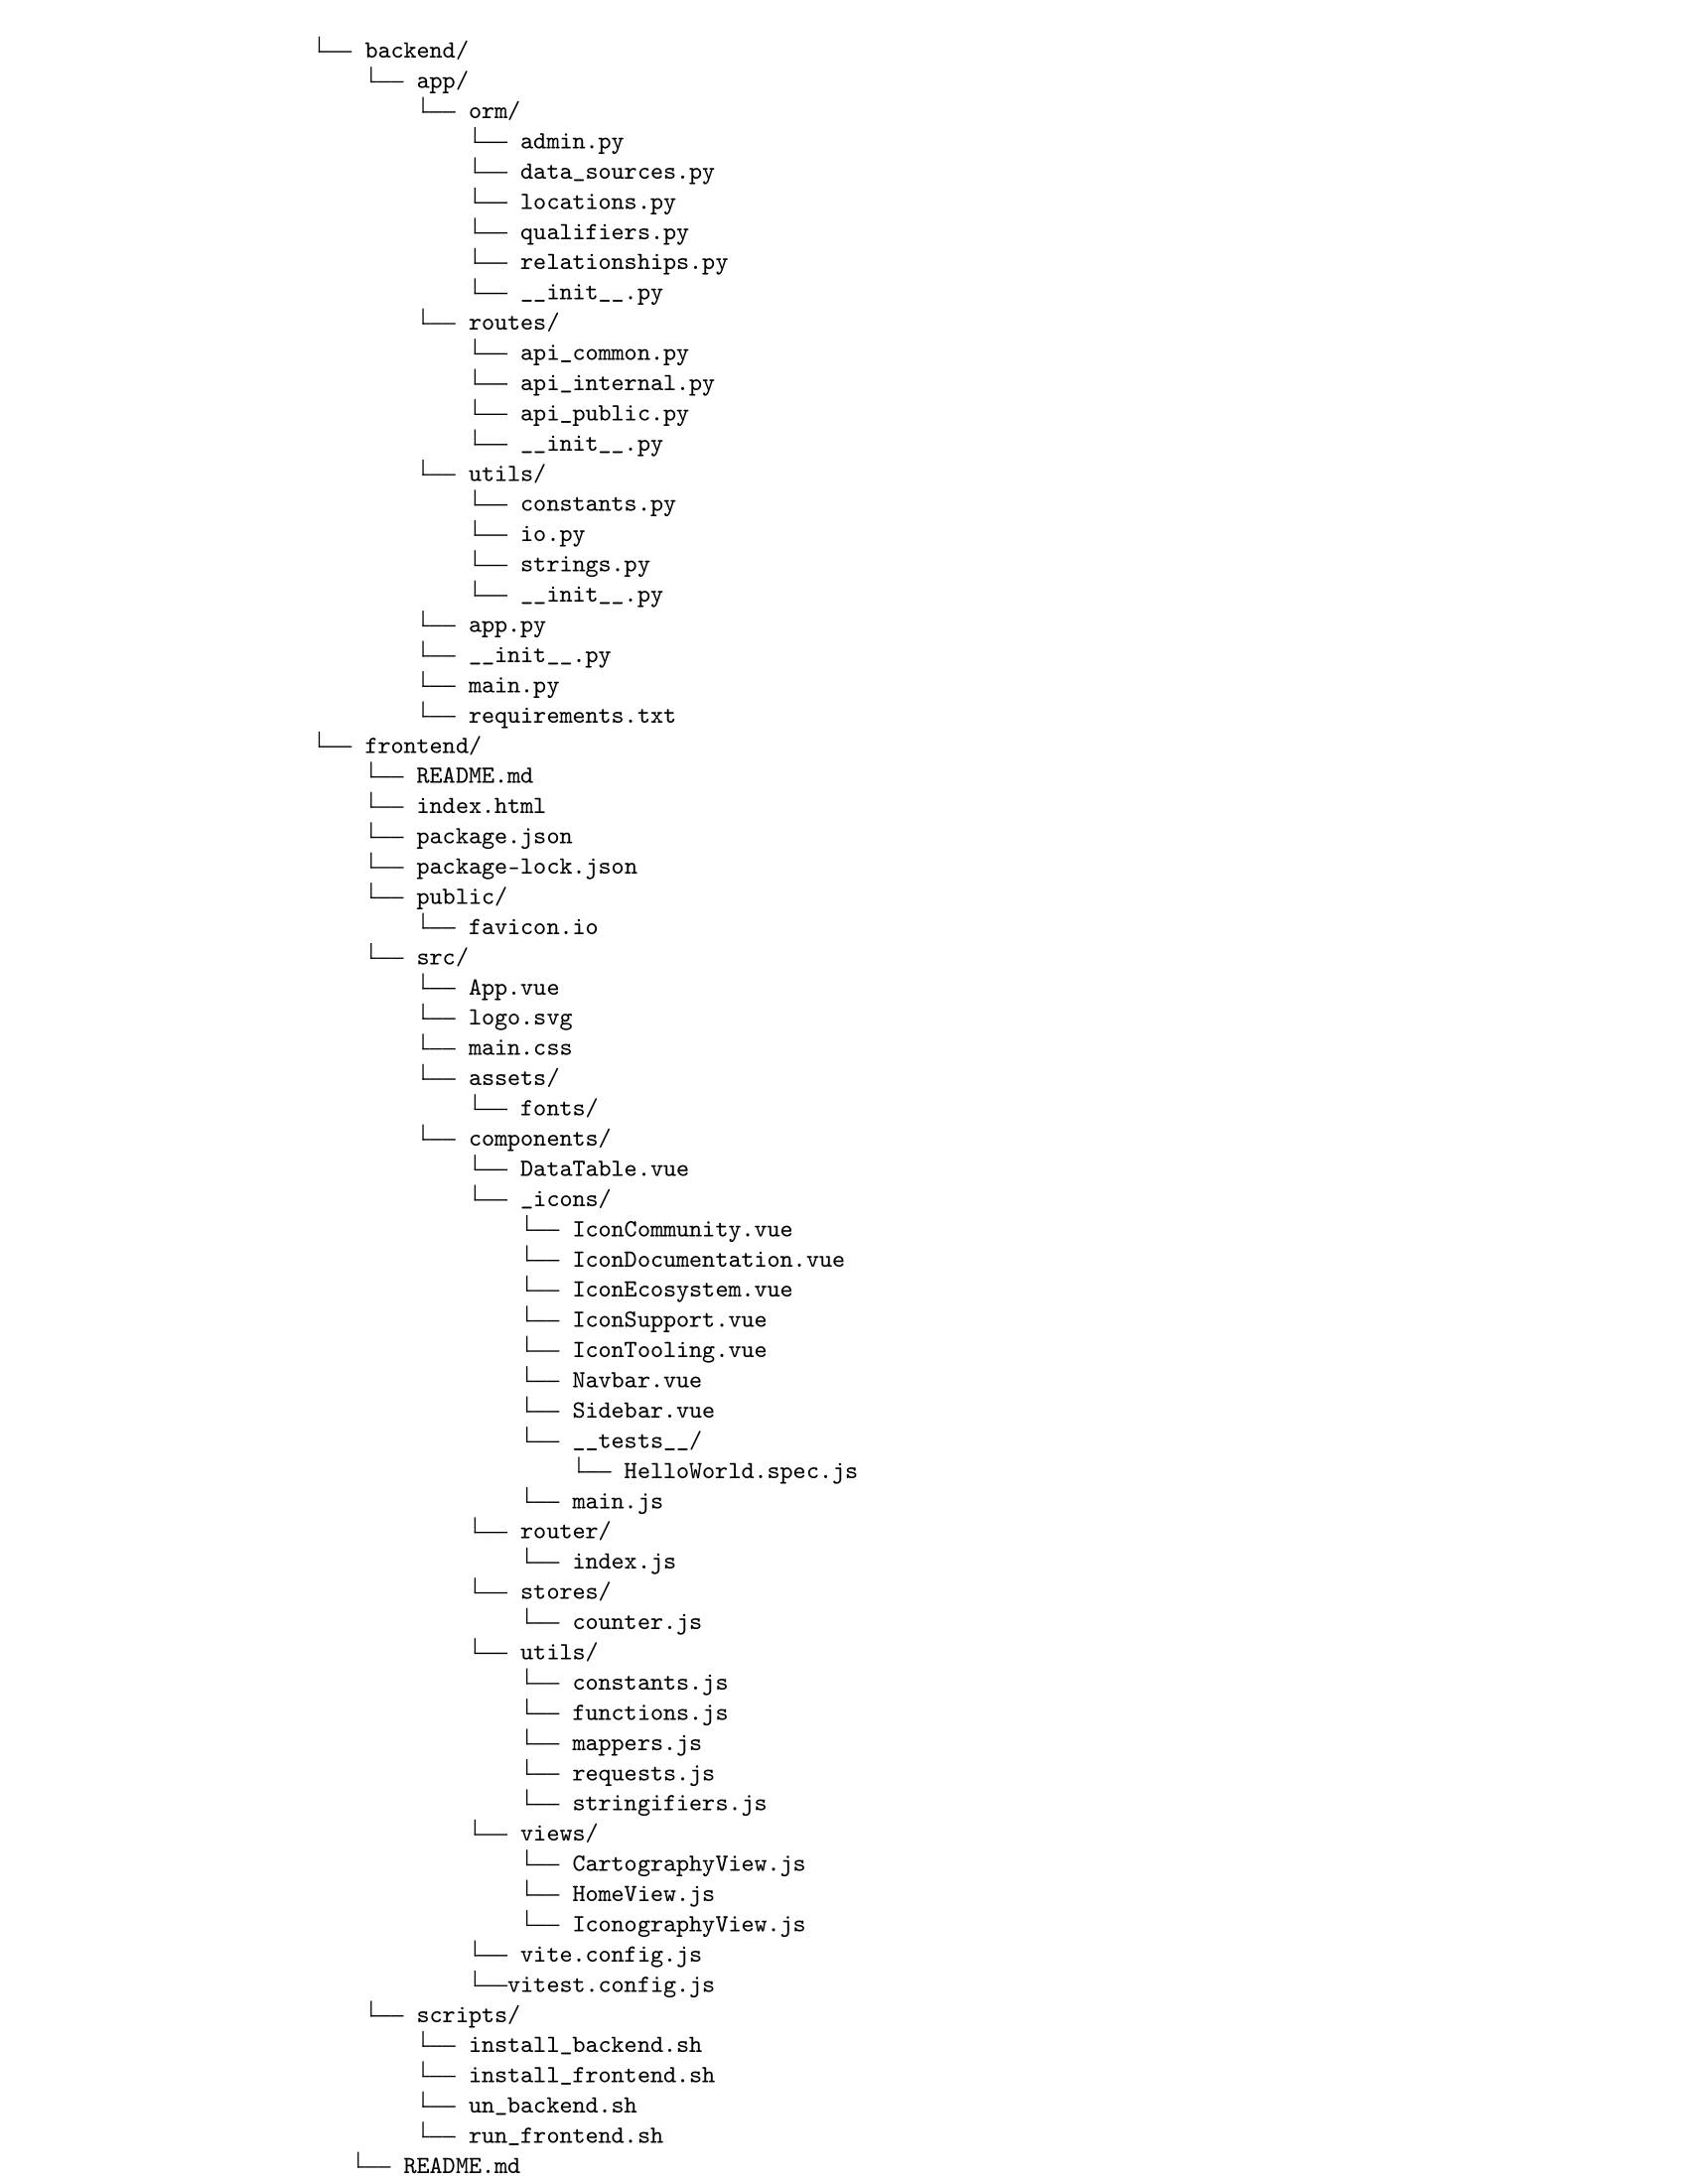
\includegraphics[width=1.1\linewidth]{annexes/architecture_appli.png}
    \caption{Architecture détaillée de l'application}
    \label{fig:archi-détaillée}
\end{figure}
%%%%%%%%%%%%%%%%%%
\chapter{Requêtes SQL et graphes pgAdmin}\label{chapter:sql}
%%%%%%%%%%%%%%%%%%%%%%%%%%%%
%LIEU
%%%%%%%%%%%%%%%%%%%%%%%%%%%%
\section{Le lieu}
%%%%%%%%%%%%%%%%%%%%%%%%%%%%
\subsection{Répartition des sources iconographiques (>100) par lieu}
\begin{lstlisting}[language=SQL, caption=Requête SQL pour nombre d'iconographies par lieu > 100]
SELECT place.id, place.id_richelieu,  
COUNT(r_iconography_place.id_iconography) AS total_icono_lieu 
FROM place 
JOIN r_iconography_place 
ON place.id = r_iconography_place.id_place 
JOIN iconography  
ON r_iconography_place.id_iconography = iconography.id 
GROUP BY place.id 
HAVING COUNT (*) > 100
ORDER BY total_icono_lieu desc; \end{lstlisting}

\begin{figure}[h!]
    \centering
    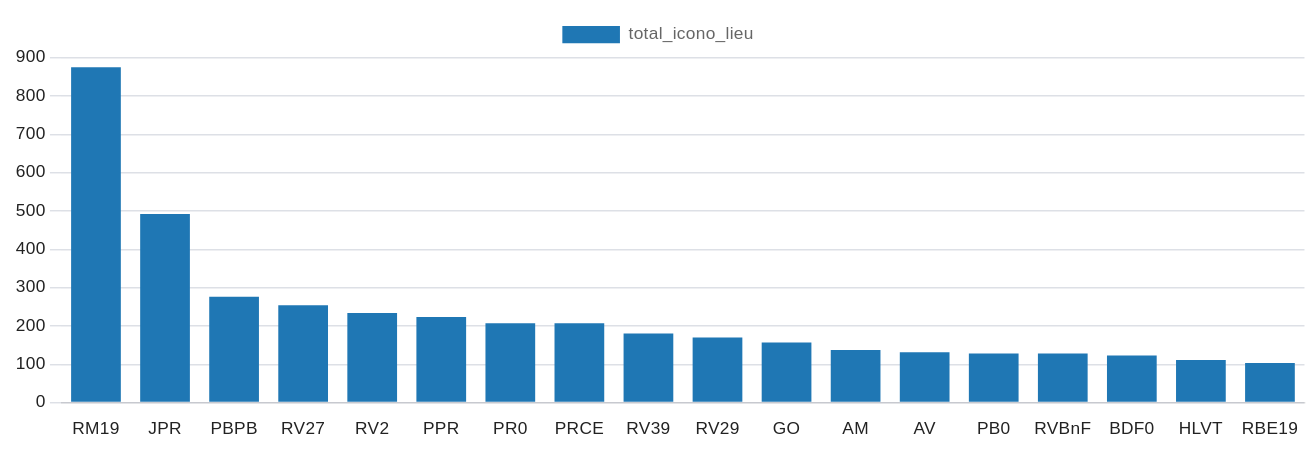
\includegraphics[width=1\linewidth]{images/graphiques/nb_icono_lieu_>100.png}
    \caption{Nombre d'iconographie par lieu (avec au moins 100 documents)}
    \label{fig:nb_icono_lieu>100}
\end{figure}    

\newpage
%%%%%%%%%%%%%%%%%%%%%%%%%%%%
\subsection{Répartition des sources cartographiques par lieu}
\begin{lstlisting}[language=SQL, caption=Requête SQL pour répartition des sources cartographiques par lieu]
SELECT place.id, place.id_richelieu,  
COUNT(r_cartography_place.id_cartography) AS total_carto_parcelle 
FROM place 
JOIN r_cartography_place 
ON place.id = r_cartography_place.id_place 
JOIN cartography  
ON r_cartography_place.id_cartography = cartography.id 
GROUP BY place.id 
ORDER BY total_carto_parcelle desc;\end{lstlisting}
\begin{figure}[h!]
    \centering
    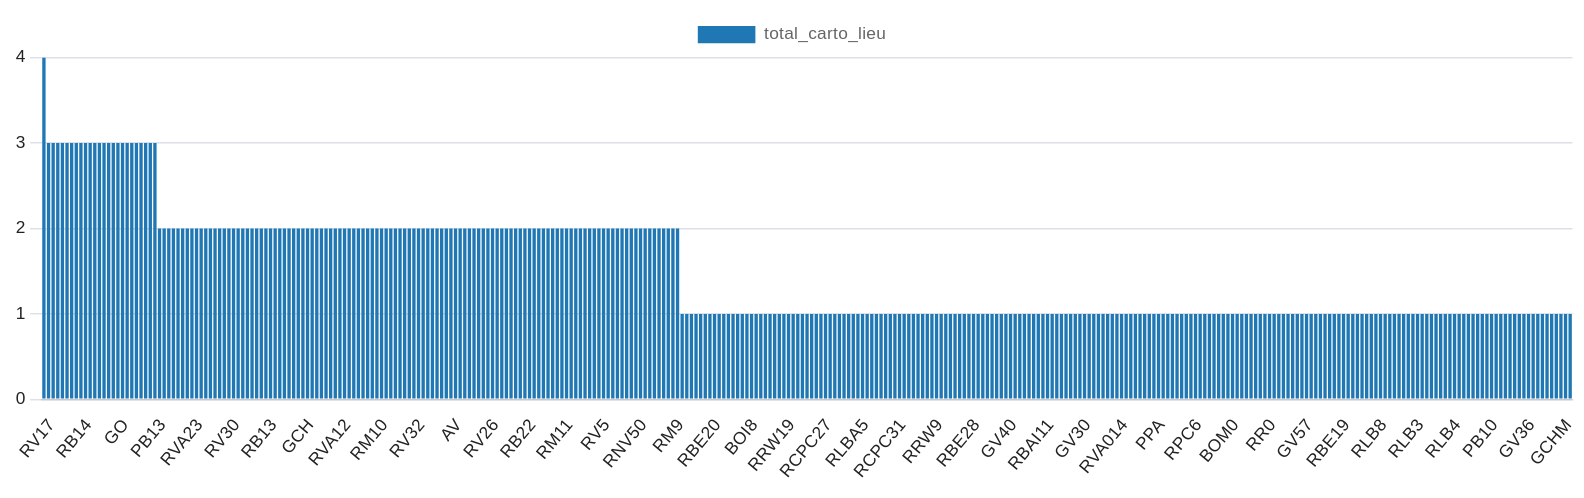
\includegraphics[width=1\linewidth]{images/graphiques/nb_carto_lieu_barChart.png}
    \caption{Nombre de sources cartographiques par lieu}
    \label{fig:nb_carto_lieu}
\end{figure}         

\begin{lstlisting}[language=SQL, caption=Reuquête SQL sur les lieux par nombre de documents cartographiques]
SELECT 
    lieu AS total_carto_lieu, 
    COUNT(id_richelieu) AS nombre_id_richelieu
FROM (
    SELECT place.id_richelieu, 
           COUNT(r_cartography_place.id_cartography) AS lieu 
    FROM place 
    JOIN r_cartography_place 
    ON place.id = r_cartography_place.id_place 
    JOIN cartography  
    ON r_cartography_place.id_cartography = cartography.id 
    GROUP BY place.id_richelieu 
) AS subquery
GROUP BY lieu
ORDER BY lieu;\end{lstlisting}

\begin{figure}[h!]
    \centering
    
\includegraphics[width=1\linewidth]{images/graphiques/repartition_lieux_nb_carto_lieu_pie.png}
    \caption{Répartition total des lieux en fonction du nombre de documents cartographiques par lieu.}
    \label{fig:repartition_carto_lieu}
\end{figure}

\begin{table}[h!]
    \centering
    \begin{tabular}{|l|r|}
        \toprule
        \textbf{Nb source carto} & \textbf{Nb lieux} \\
        \midrule
        1 & 193 \\
        2 & 113 \\
        3 & 24 \\
        4 & 1 \\
        \bottomrule
    \end{tabular}
    \label{tab:repartition_lieu_carto}
    \caption{Répartition totale du nombre de source cartographique par lieu.}
\end{table}

\newpage
%%%%%%%%%%%%%%%%%%%%%%%%%%%%
\subsection{Répartition toutes sources confondues par lieu}
\begin{lstlisting}[language=SQL, caption=Requête SQL pour répartition des sources par lieu]
SELECT subquery.id, subquery.id_richelieu, subquery.total_sources_lieu
FROM (
    SELECT p.id, p.id_richelieu,  
        COALESCE(carto.total_carto_lieu, 0) + COALESCE(icono.total_icono_lieu, 0) AS total_sources_lieu
    FROM place p
    LEFT JOIN (
        SELECT place.id, 
        COUNT(r_cartography_place.id_cartography) AS total_carto_lieu 
        FROM place 
        JOIN r_cartography_place 
        ON place.id = r_cartography_place.id_place 
        JOIN cartography  
    	ON r_cartography_place.id_cartography = cartography.id 
        GROUP BY place.id
    ) AS carto 
    ON p.id = carto.id
    LEFT JOIN (
        SELECT place.id, 
        COUNT(r_iconography_place.id_iconography) AS total_icono_lieu 
        FROM place 
        JOIN r_iconography_place 
        ON place.id = r_iconography_place.id_place 
        JOIN iconography  
        ON r_iconography_place.id_iconography = iconography.id 
        GROUP BY place.id
    ) AS icono 
    ON p.id = icono.id
) AS subquery
ORDER BY subquery.total_sources_lieu DESC;\end{lstlisting}

\begin{figure}[h!]
    \centering
    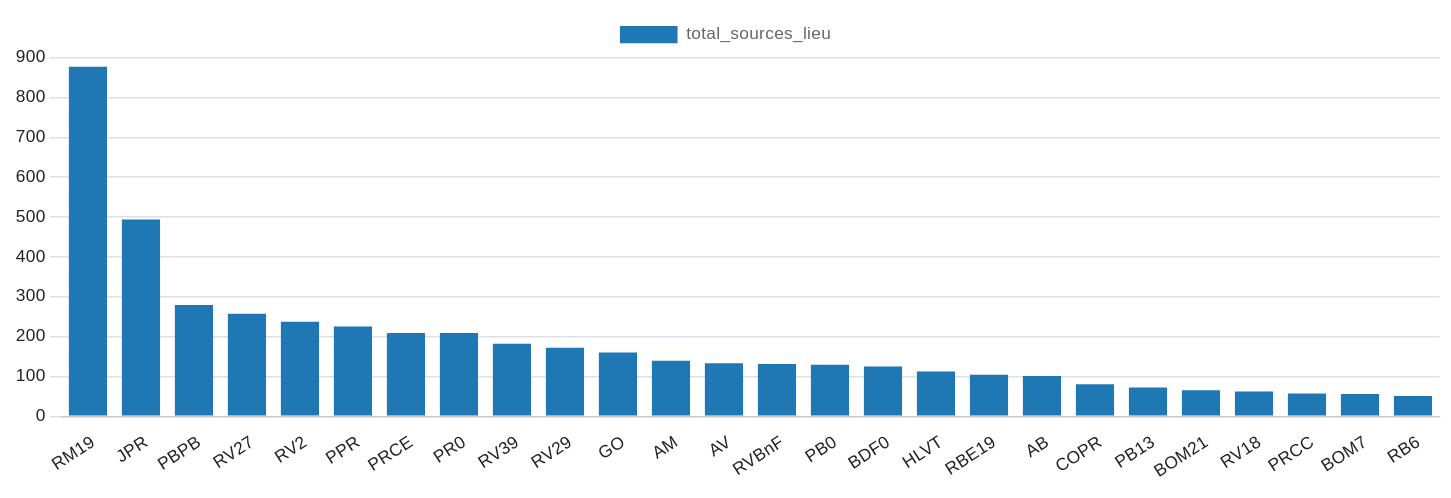
\includegraphics[width=1\linewidth]{images/graphiques/total_source_lieu.png}
    \caption{Répartition totale des sources par lieu}
    \label{fig:total_source_lieu}
\end{figure}
\newpage
%%%%%%%%%%%%%%%%%%%%%%%%%%%%
%CORPUS
%%%%%%%%%%%%%%%%%%%%%%%%%%%%
\section{Les corpus documentaires}
\subsection{La répartition des sources par institution}
\begin{lstlisting}[language=SQL, caption=Requête SQL pour nombre total de sources par institution]
SELECT 
    i.entry_name AS nom_institution,
    COALESCE(icono.nb_iconographie, 0) AS nb_iconographie,
    COALESCE(carto.nb_cartographie, 0) AS nb_cartographie,
    COALESCE(icono.nb_iconographie, 0) + COALESCE(carto.nb_cartographie, 0) AS total_resources
FROM institution AS i
LEFT JOIN (
    SELECT r.id_institution, COUNT(r.id_iconography) AS nb_iconographie
    FROM r_institution AS r 
    JOIN iconography AS ic 
        ON r.id_iconography = ic.id 
    GROUP BY r.id_institution
) AS icono 

ON i.id = icono.id_institution

LEFT JOIN (
    SELECT r.id_institution, COUNT(r.id_cartography) AS nb_cartographie 
    FROM r_institution AS r 
    JOIN cartography AS ic 
        ON r.id_cartography = ic.id 
    GROUP BY r.id_institution
) AS carto 

ON i.id = carto.id_institution
WHERE COALESCE(icono.nb_iconographie, 0) + COALESCE(carto.nb_cartographie, 0) > 50
ORDER BY total_resources DESC; \end{lstlisting}
\begin{figure}[h!]
    \centering
    \includegraphics[width=1\linewidth]{images/graphiques/total_source_institution.png}
    \caption{Nombre total de sources par institution}
    \label{fig:total_sources_institution}
\end{figure}

% \begin{table}
% \begin{tabular}{|l|r|r|r|}
% \centering
% \textbf{Nom de l'institution} & \textbf{Nb iconographie} & \textbf{Nb cartographie} & \textbf{Total source} \\
% Paris Musées & 1438 & 22 & 1460 \\
% Musée Carnavalet & 1333 & 0 & 1333 \\
% Bibliothèque nationale de France & 1312 & 0 & 1312 \\
% Bibliothèques spécialisées de la Ville de Paris & 928 & 0 & 928 \\
% Bibliothèque historique de la Ville de Paris & 827 & 0 & 827 \\
% British Museum & 295 & 0 & 295 \\
% Archives de Paris & 46 & 239 & 285 \\
% Archives nationales & 0 & 208 & 208 \\
% Institut national d'histoire de l'art & 162 & 0 & 162 \\
% Bibliothèque Forney & 73 & 0 & 73 \\
% \end{tabular}
% \caption{Répartition totale des sources par institution}
% \label{tab:resources}
% \end{table}

\newpage
%%%%%%%%%%%%%%%%%%%%%%%%%%%%
\subsection{La répartition des iconographiques par medium}
\begin{lstlisting}[language=SQL, caption=Requête SQL pour nombre d'iconographies par technique]
SELECT 
    CASE 
    WHEN EXISTS (
        SELECT 1 
        FROM unnest(technique) AS t
        WHERE t ~* 'photographie'
        ) THEN 'photographie'
        WHEN EXISTS (
        SELECT 1 
        FROM unnest(technique) AS t
        WHERE t ~* 'gravure' OR t ~* 'estampe' OR t ~* 'lithographie'
        ) THEN 'estampe'
        WHEN EXISTS (
        SELECT 1 
        FROM unnest(technique) AS t
        WHERE t ~* 'dessin'
        ) THEN 'dessin'
        WHEN EXISTS (
        SELECT 1 
        FROM unnest(technique) AS t
        WHERE t ~* 'négatif'
        ) THEN 'négatif'
        WHEN EXISTS (
        SELECT 1 
        FROM unnest(technique) AS t
        WHERE t ~* 'plan'
        ) THEN 'plan'
        WHEN EXISTS (
        SELECT 1 
        FROM unnest(technique) AS t
        WHERE t ~* 'tableau' OR t ~* 'peinture'
        ) THEN 'peinture'
        ELSE array_to_string(technique, ', ')
        END AS type_regroupe,
    COUNT(*) AS nombre
    FROM iconography
GROUP BY type_regroupe
HAVING COUNT(*) > 10
ORDER BY nombre DESC; \end{lstlisting}

\begin{figure}[h!]
    \centering
    \includegraphics[width=1\linewidth]{images/graphiques/nb_icono_technique>10.png}
    \caption{Nombre d'iconographie par technique (en excluant celles de moins de 10 occurrences)}         \label{fig:nb_icono_technique}
\end{figure}

\begin{table}[h!]
    \centering
    \begin{tabular}{|l|r|}
        \toprule
        \textbf{Technique} & \textbf{Nombre} \\ \hline
        estampe        & 1436 \\ 
        photographie   & 1357 \\ 
        dessin         & 401  \\ 
        \texttt{NULL}  & 206  \\ 
        imprimé        & 179  \\ 
        carte postale  & 147  \\ 
        négatif        & 108  \\
        aquarelle      & 99   \\
        jeton          & 31   \\
        affiche        & 28   \\
        médaille       & 23   \\
        peinture       & 21   \\
        autochrome     & 19   \\
        sculpture      & 18   \\
        plan           & 18   \\ 
        \midrule
        \textbf{Total} & 4091 \\
        \bottomrule
    \end{tabular}
    \caption{Répartition des types d'iconographies}
    \label{tab:repartition_iconographies}
\end{table}

\newpage
%%%%%%%%%%%%%%%%%%%%%%%%%%%%
%TEMPS
%%%%%%%%%%%%%%%%%%%%%%%%%%%%
\section{Le temps}
\subsection{La répartition temporelle des sources : par intervalle de 50 ans}
\begin{lstlisting}[language=SQL, caption=Requête SQL pour nombre de sources par date (50 ans)]
SELECT
    periode,
    SUM(nombre_documents) AS nombre_documents,
    SUM(nombre_iconographies) AS nombre_iconographies,
    SUM(nombre_cartographies) AS nombre_cartographies
FROM (
    SELECT 
        CASE 
            WHEN iconography.date && int4range(1200, 1750) THEN 'avant1750'
            WHEN iconography.date && int4range(1750, 1800) THEN '1750-1800'
            WHEN iconography.date && int4range(1800, 1850) THEN '1800-1850'
            WHEN iconography.date && int4range(1850, 1900) THEN '1850-1900'
            WHEN iconography.date && int4range(1900, 1950) THEN '1900-1950'
            WHEN iconography.date && int4range(1950, 2100) THEN 'après1950'
        END AS periode,
        COUNT(*) AS nombre_documents,
        COUNT(*) AS nombre_iconographies,
        0 AS nombre_cartographies
    FROM 
        iconography
    GROUP BY 
        periode

    UNION ALL

    SELECT 
        CASE 
            WHEN cartography.date && int4range(1200, 1750) THEN 'avant1750'
            WHEN cartography.date && int4range(1750, 1800) THEN '1750-1800'
            WHEN cartography.date && int4range(1800, 1850) THEN '1800-1850'
            WHEN cartography.date && int4range(1850, 1900) THEN '1850-1900'
            WHEN cartography.date && int4range(1900, 1950) THEN '1900-1950'
            WHEN cartography.date && int4range(1950, 2100) THEN 'après1950'
        END AS periode,
        COUNT(*) AS nombre_documents,
        0 AS nombre_iconographies,
        COUNT(*) AS nombre_cartographies
    FROM 
        cartography
    GROUP BY 
        periode
) AS combined_results
GROUP BY 
    periode
ORDER BY 
    CASE 
        WHEN periode = 'avant 1750' THEN 1
        WHEN periode = '1750-1800' THEN 2
        WHEN periode = '1800-1850' THEN 3
        WHEN periode = '1850-1900' THEN 4
        WHEN periode = '1900-1950' THEN 5
        WHEN periode = 'après 1950' THEN 6
    END; \end{lstlisting}
    
\begin{figure}[h!]
    \centering
    \includegraphics[width=0.75\linewidth]{images/graphiques/total_source_date_50.png}
    \caption{Nombre total de sources par date (intervalle de 50 ans)}
    \label{fig:total_sources_date50}
\end{figure}

\newpage
%%%%%%%%%%%%%%%%%%%%%%%%%%%%
\subsection{La répartition temporelle des sources : par intervalle de 10 ans}
\begin{lstlisting}[language=SQL, caption=Requête SQL pour nombre de sources par date (10 ans)]
SELECT COALESCE(c.periode, i.periode) AS periode, COALESCE(nb_carto_periode_10ans, 0) AS nb_carto_periode_10ans, COALESCE(nb_icono_periode_10ans, 0) AS nb_icono_periode_10ans
FROM 
    (SELECT CASE 
        WHEN cartography.date && int4range(1200, 1750) THEN '> 1750' 
        WHEN cartography.date && int4range(1750, 1760) THEN '1750-1760' 
        WHEN cartography.date && int4range(1760, 1770) THEN '1760-1770' 
        WHEN cartography.date && int4range(1770, 1780) THEN '1770-1780' 
        WHEN cartography.date && int4range(1780, 1790) THEN '1780-1790' 
        WHEN cartography.date && int4range(1790, 1800) THEN '1790-1800' 
        WHEN cartography.date && int4range(1800, 1810) THEN '1800-1810' 
        WHEN cartography.date && int4range(1810, 1820) THEN '1810-1820' 
        WHEN cartography.date && int4range(1820, 1830) THEN '1820-1830' 
        WHEN cartography.date && int4range(1830, 1840) THEN '1830-1840' 
        WHEN cartography.date && int4range(1840, 1850) THEN '1840-1850' 
        WHEN cartography.date && int4range(1850, 1860) THEN '1850-1860' 
        WHEN cartography.date && int4range(1860, 1870) THEN '1860-1870' 
        WHEN cartography.date && int4range(1870, 1880) THEN '1870-1880' 
        WHEN cartography.date && int4range(1880, 1890) THEN '1880-1890' 
        WHEN cartography.date && int4range(1890, 1900) THEN '1890-1900' 
        WHEN cartography.date && int4range(1900, 1910) THEN '1900-1910' 
        WHEN cartography.date && int4range(1920, 1930) THEN '1920-1930' 
        WHEN cartography.date && int4range(1930, 1940) THEN '1930-1940' 
        WHEN cartography.date && int4range(1940, 1950) THEN '1940-1950' 
        WHEN cartography.date && int4range(1950, 2100) THEN '< 1950' 
        END AS periode, 
        COUNT(*) AS nb_carto_periode_10ans
    FROM cartography 
    GROUP BY periode 
    ORDER BY periode) c
FULL OUTER JOIN 
    (SELECT CASE 
        WHEN iconography.date && int4range(1200, 1750) THEN '> 1750' 
        WHEN iconography.date && int4range(1750, 1760) THEN '1750-1760' 
        WHEN iconography.date && int4range(1760, 1770) THEN '1760-1770' 
        WHEN iconography.date && int4range(1770, 1780) THEN '1770-1780' 
        WHEN iconography.date && int4range(1780, 1790) THEN '1780-1790' 
        WHEN iconography.date && int4range(1790, 1800) THEN '1790-1800' 
        WHEN iconography.date && int4range(1800, 1810) THEN '1800-1810' 
        WHEN iconography.date && int4range(1810, 1820) THEN '1810-1820' 
        WHEN iconography.date && int4range(1820, 1830) THEN '1820-1830' 
        WHEN iconography.date && int4range(1830, 1840) THEN '1830-1840' 
        WHEN iconography.date && int4range(1840, 1850) THEN '1840-1850' 
        WHEN iconography.date && int4range(1850, 1860) THEN '1850-1860' 
        WHEN iconography.date && int4range(1860, 1870) THEN '1860-1870' 
        WHEN iconography.date && int4range(1870, 1880) THEN '1870-1880' 
        WHEN iconography.date && int4range(1880, 1890) THEN '1880-1890' 
        WHEN iconography.date && int4range(1890, 1900) THEN '1890-1900' 
        WHEN iconography.date && int4range(1900, 1910) THEN '1900-1910' 
        WHEN iconography.date && int4range(1920, 1930) THEN '1920-1930' 
        WHEN iconography.date && int4range(1930, 1940) THEN '1930-1940' 
        WHEN iconography.date && int4range(1940, 1950) THEN '1940-1950' 
        WHEN iconography.date && int4range(1950, 2100) THEN '< 1950' 
        END AS periode, 
        COUNT(*) AS nb_icono_periode_10ans
    FROM iconography 
    GROUP BY periode 
    ORDER BY periode) i
ON c.periode = i.periode
ORDER BY periode; \end{lstlisting}

\begin{figure}[h!]
    \centering
    \includegraphics[width=1\linewidth]{images/graphiques/total_source_date_10.png}
    \caption{Total des sources par date (intervalle de 10 ans)}
    \label{fig:total_sources_date10}
\end{figure}
%%%%%%%%%%%%%%%%%%
\chapter{Les fonds de cartes historiques}

\begin{figure}
    \begin{subfigure}{.5\textwidth}
      \centering
      \includegraphics[width=0.9\linewidth]{images/plan-verniquet.png}
      \caption{Plan Verniquet (1791)}
      \label{fig:verniquet}
    \end{subfigure}
    \begin{subfigure}{.5\textwidth}
      \centering
      \includegraphics[width=0.9\linewidth]{images/plan-vasserot.png}
      \caption{Atlas Vasserot (1810-1836)}
      \label{fig:vasserot}
    \end{subfigure}
    \begin{subfigure}{.5\textwidth}
      \centering
      \includegraphics[width=0.9\linewidth]{images/plan-1812.png}
      \caption{Plan de 1812}
      \label{fig:1812}
    \end{subfigure}
    \begin{subfigure}{.5\textwidth}
      \centering
      \includegraphics[width=.9\linewidth]{images/plan-parcellaire.png}
      \caption{Plan parcellaire de 1900}
      \label{fig:zoom-16}
    \end{subfigure}
    \begin{subfigure}{.5\textwidth}
      \centering
      \includegraphics[width=.9\linewidth]{images/plan-1943.png}
      \caption{Plan de 1943}
      \label{fig:1943}
    \end{subfigure}
\caption{Les fonds de cartes historiques du projet Richelieu, \mhd.}
\label{fig:carto-histo}
\end{figure}
\newpage{\pagestyle{empty}\cleardoublepage}
%%%%%%%%%%%%%%%%%%
\chapter{La plateforme Galligeo}
\begin{figure}
    \centering
    \includegraphics[width=1\linewidth]{annexes/plateforme-galligeo.png}
    \caption{Visuel de la plateforme Galligeo}
    \label{fig:platefomre-galligeo}
\end{figure}
\begin{figure}
    \centering
    \includegraphics[width=1\linewidth]{annexes/point-de-contrôle.png}
    \caption{Poins de contrôle sur carte 1943}
    \label{fig:points-de-contrôle}
\end{figure}
\begin{figure}
    \centering
    \includegraphics[width=1\linewidth]{annexes/résultat-géoréférencement.png}
    \caption{Résultat géoréférencement}
    \label{fig:résultat-géoréférencement}
\end{figure}
%%%%%%%%%%%%%%%%%%
\chapter{La plateforme pour générer emprise du quartier en GeoJSON}
\begin{figure}
    \centering
    \includegraphics[width=1\linewidth]{annexes/geojson.png}
    \caption{GeoJSON empreinte du quartier}
    \label{fig:geojson-quartier}
\end{figure}
%%%%%%%%%%%%%%%%%%
\chapter{Captures d'écrans de la carte développée}
\begin{figure}
    \centering
    \includegraphics[width=1\linewidth]{annexes/carte-parcelle.png}
    \caption{Capture d'écran de la carte avec l'ensemble des parcelles \textit{HeatMap}}
    \label{fig:carte-parcelle}
\end{figure}

\begin{figure}
    \centering
    \includegraphics[width=1\linewidth]{annexes/carte-pbpb.jpeg}
    \caption{Capture d'écran de la carte avec clic sur un bâtiment de la Place de la Bourse}
    \label{fig:carte-pb}
\end{figure}

\begin{figure}
    \centering
    \includegraphics[width=1\linewidth]{annexes/carte-pr.jpeg}
    \caption{Capture d'écran de la carte avec clic sur un bâtiment du Palais Royal}
    \label{fig:carte-pr}
\end{figure}
%%%%%%%%%%%%%%%%%%
\chapter{Script JavaScript}
\begin{lstlisting}[language=HTML, caption=Script JavaScript]
<script>    
    //Déclarer la carte sur Paris et en enlever le zoomcontrol par défaut
    var map = L.map('map', {zoomControl:false}).setView([48.866772, 2.338935], 12);    
    
    //Changer l'attribution de la carte      
    map.attributionControl.setPrefix('<a href="https://leafletjs.com/">Leaflet</a>');
    map.attributionControl.addAttribution('&copy; <a href="https://quartier-richelieu.inha.fr/">Richelieu.Histoire du quartier</a>, Marina Hervieu, 2024');
    map.attributionControl.setPosition('bottomleft');

   
    //Pour placer l'échelle
    L.control.scale({position:'bottomleft'}).addTo(map);

    //Pour placer control zoom
    L.control.zoom({position:'bottomleft'
    , opacity: 1
    , maxZoom: 19.5
    , minZoom: 12
    }).addTo(map);
  
    //Pour le fond de carte par défaut
    var contemporain = L.tileLayer('https://server.arcgisonline.com/ArcGIS/rest/services/World_Topo_Map/MapServer/tile/{z}/{y}/{x}', {
      opacity: 1
      , maxZoom: 18
      , minZoom: 12}).addTo(map);
    
    //Emprise GeoJSON du quartier  
    var zone = {
      "type": "FeatureCollection",
      "features": [
      {
        "type": "Feature",
        "properties": {},
        "geometry": {
          "type": "MultiPolygon",
          "coordinates": [
          [
          [
          [
          -9.308577500591156,
          51.96179459849796
          ],
          [
          -9.308577500591156,
          41.03936743552862
          ],
          [
          ...
          ],
            [
              2.3431082580363807,
              48.87146697188524
            ]
          ]
          ]
          ]
        }
      }
      ]
    };
    
    //Pour changer le style du GeoJSON
    var myStyle = {
      "color": "#121212",
      "opacity": 1,
      "stroke": false,
      "stroke-linejoin" :"round"
    };
    L.geoJSON(zone, {style : myStyle}).addTo(map);
    

    // Pour sélectionner les id de la page d'info
    document.addEventListener('DOMContentLoaded', function() {
      const infoPage = document.getElementById('infoPage');
      const closeBtn = document.getElementById('closeBtn');
      const infoIcon = document.getElementById('infoIcon');
      
      //Afficher la page d'informations avec faible opacité
      infoPage.style.opacity = '0.8';
      
      // Ajouter un événement pour le bouton "fermer"
      closeBtn.addEventListener('click', function() {
        // Fermer la page d'informations
        infoPage.style.opacity = '0';
        setTimeout(() => {
          infoPage.style.display = 'none';
          infoIcon.style.display = 'block';
        }, 500);
      });
      
      // Afficher la page d'info quand l'icone info est cliquée
      infoIcon.addEventListener('click', function() {
        infoPage.style.display = 'flex';
        setTimeout(() => {
          infoPage.style.opacity = '0.9';
        }, 10);
        infoIcon.style.display = 'none';
      });
    });
    
    // Effet waouh
    setTimeout(function(){
      map.flyTo([48.866772, 2.338935], 16);
    }, 5000);
    
    
    // Variable optimisée des fonds de carte
    var tileLayers = {
      '1. Plan Verniquet (1791)': 'https://tile.ptm.huma-num.fr/tiles/ark/highres/12148/btv1b55013275x/{z}/{x}/{y}.webp',
      '2. Atlas Vasserot (1810-1836)': 'https://tile.maps.huma-num.fr/uc2usU/d/Alpage_Vasserot_1830/{z}/{x}/{y}.png',
      '3. 1812': 'https://tile.ptm.huma-num.fr/tiles/ark/highres/12148/btv1b530851375/{z}/{x}/{y}.webp',
      '4. Cadastre municipal (1900)': 'https://tile.maps.huma-num.fr/uc2usU/d/MOSA_1900_PARIS/{z}/{x}/{y}.png',
      '5. 1943': 'https://tile.ptm.huma-num.fr/tiles/ark/highres/12148/btv1b53121232b/{z}/{x}/{y}.webp', 
    }
    
    // Variable pour fond de carte contemporain par défaut 
    var baseMap = {
      'Carte contemporaine': contemporain
    };
    
    // Variable pour stocker les couches historiques
    var overlayLayers = {};
    
    // Boucle qui parcourt chaque clé de l'objet tileLayers pour ajouter les couches historiques (tileLayer)
    // chaque clé représente à fond de carte à superposer sur la carte par défaut        
    for (var name in tileLayers) {
      
      // variable tileLayer éponyme de la fonction leaflet pour créer une couche de tuiles à partir de l'URL fournie (la valeur de la clé)
      // opacity est utilisé ici pour indiqué que la couche doit être complètement opaque (from 0 to 1)
      var tileLayer = L.tileLayer(tileLayers[name], {
        opacity: 1
        , interactive : true
        , maxZoom: 18.5
        , minZoom: 12
      });
      
      // puis ajouter la valeur de la clé name à la variable qui stocke les couches overlayLayers
      overlayLayers[name] = tileLayer;
    }
    
    // Contrôle pour basculer d'une couche à une autre, baseMap reste par défaut et s'y ajoute les overlayLayers
    var layersControl = L.control.layers(baseMap, overlayLayers).addTo(map);
    layersControl.setPosition('bottomright');
    
   
    //Bouton "Légende"
    document.querySelector('.legende').addEventListener('click', function() {
      const sidebar = document.getElementById('sidebar');
      const legendeIcon = document.getElementById('Legende');
      
      if (sidebar.classList.contains('open')) {
        sidebar.classList.remove('open');
        legendeIcon.textContent = '>';  // Revenir à l'icône ">"
        setTimeout(function() {
          sidebar.style.display = 'none';
        }, 300); // Durée de la transition CSS
      } else {
        sidebar.style.display = 'block';
        setTimeout(function() {
          sidebar.classList.add('open');
        }, 10);
        legendeIcon.textContent = '<';  // Changer l'icône en "<"
      }
    });
    
    // Contrôle d'opacité
    var currentLayer = null;
    
    // appeler l'élément html créé plus tôt et y ajouter un événement input
    // déclarer une variable qui va stocker la valeur d'opacité
    // si la valeur change, la fonction ajuste met à jour l'opacité de la layer en cours d'utilisation
    document.getElementById('opacity-slider').addEventListener('input', function(event) {
      var opacity = event.target.value;
      if (currentLayer) {
        currentLayer.setOpacity(opacity);
      }
    });
    
    // Ecouteurs d'événements ajoutés/attachés à la carte pour mettre à jour (ajouter ou supprimer) le layer
    // exécution de la fonction de rappel
    map.on('overlayadd', function(event) {
      //variable qui contient la couche ajoutée
      //overlayLayers clé : valeur === nom des couches : objets de L.tileLayer
      currentLayer = overlayLayers[event.name];
      currentLayer.setOpacity(document.getElementById('opacity-slider').value);
    });
    
    map.on('overlayremove', function(event) {
      if (currentLayer === overlayLayers[event.name]) {
        currentLayer = null;
      }
    });
   
   // function Fetch données de Place
  fetch('/api/places', {
  method: 'GET',
  mode: 'cors' })
    .then(response => response.json())
    .then(data => {
      L.geoJSON(data, {
        style: function (feature) {
          var count = feature.properties.iconography_count;
          var color = getColorForCount(count);
          return { color: color };
        },
        onEachFeature: function (feature, layer) {
          layer.on('mouseover', function () {
            layer.setStyle({
              color: darkenColor(layer.options.color),
            });
          });

          layer.on('mouseout', function () {
            layer.setStyle({
              color: getColorForCount(feature.properties.iconography_count),
            });
          });

          layer.on('click', function () {
            layer.setStyle({ color : 'yellow' });
            showImageGallery(feature.properties.id, layer, feature.properties.iconographies);
          });
        }
      }).addTo(map);
    })

  // Function pour obtenir la couleur basé sur un nombre limité d'icono
  function getColorForCount(count) {
    if (count > 320) return '#000000';  // More than 320 images
    if (count > 160) return '#4b0082';  // More than 160 images
    if (count > 80) return '#800080';   // More than 80 images
    if (count > 40) return '#ff0000';   // More than 40 images
    if (count > 20) return '#ff4500';   // More than 20 images
    if (count > 10) return '#ff7f50';   // More than 10 images
    if (count > 5) return '#ffddc1';    // More than 5 images
    return '#ffffff';                   // Less than 5 images
  }

  //Function créer la légende
  function createLegend() {
  var legend = document.getElementById('legend-content');
  
  if (!legend) {
    console.error("La légende n'est pas là!");
    return;
  }

  console.log("La légende est là, création en cours");

  // Nettoyer les éléments si précédent
  legend.innerHTML = '';

  //Eléments de la légende (rectangle de couleur)
  var legendItems = [
    ['#000000', 'Plus de 320 images par lieu'],
    ['#4b0082', 'Plus de 160 images par lieu'],
    ['#800080', 'Plus de 80 images par lieu'],
    ['#ff0000', 'Plus de 40 images par lieu'],
    ['#ff4500', 'Plus de 20 images par lieu'],
    ['#ff7f50', 'Plus de 10 images par lieu'],
    ['#ffddc1', 'Plus de 5 images par lieu'],
    ['#ffffff', 'Moins de 5 images par lieu']
  ];

  //Générer élements HTML pour la légende
  legendItems.forEach(function(item) {
    var colorBox = '<span style="display:inline-block;width:20px;height:20px;background-color:' + item[0] + ';margin-right:10px;"></span>';
    var label = '<span>' + item[1] + '</span>';
    var legendItem = '<div style="margin-bottom:5px;">' + colorBox + label + '</div>';
    legend.innerHTML += legendItem;
  });
}

  //Fonction pour fetch et afficher les images au clic sur parcelle 
  function showImageGallery(placeId, layer, iconographies) {
    if (iconographies && iconographies.length > 0) {
      var galleryHtml = '<div class="popup-gallery">';

      // Boucle pour parcourir chaque icono et afficher url et titre
      iconographies.forEach(function(iconography) {
        var sourceUrl = iconography.source_url || '';  // url de Iconography
        var title = iconography.title ? iconography.title.join(', ') : 'Untitled';  // Joindre les titres si plusieurs (à revoir pour éviter de surcharger info)

        galleryHtml += '<div class="popup-gallery-item">';
        galleryHtml += '<img src="' + sourceUrl + '" class="popup-gallery-image" alt="' + title + '"/>';  //afficher image ou lien au click droit
        galleryHtml += '<p>' + title + '</p>';  // ajouter titre en dessous de chaque image
        galleryHtml += '</div>';
      });

      galleryHtml += '</div>';

      // Engagner la galerie HTML au popup et l'ouvrir 
      layer.bindPopup(galleryHtml, { maxHeight: 300 }).openPopup();
    } else {
      // si pas d'image dispo
      layer.bindPopup('<p>Aucun image disponible pour ce lieu.</p>').openPopup();
    }
  }

  // Fonction pour changer couleur en noir au survol du lieu
  function darkenColor(color) {
    return '#333';  // noir
  }

  //Initialiser la légende au chargement de la carte 
  createLegend();
</script>
\end{lstlisting}
%%%%%%%%%%%%%%%%%%
%%%%%%%%%%%%%%%%%%
\backmatter
%\printindex
\printglossaries
\listoftables
\listoffigures
\tableofcontents
\end{document}
